\iflanguage{ngerman}
{\chapter{Ergebnisse}}
{\chapter{Results}}

\label{sec:results}

% \section{Task~1: Current-Visit Diagnosis Prediction}
% \label{sec:results-task1}

% This section reports results for Task~1 (current-visit diagnosis prediction) under the evaluation protocol in Section~\ref{sec:evaluation}. We evaluate three modelling stages (\textbf{Base}, \textbf{CodeGen}, \textbf{TextGen}) across three backbones (\texttt{Llama-3.2-1B-Instruct}, \texttt{Llama-3.1-8B-Instruct}, \texttt{Meditron-8B}). For \textbf{Base} runs, LoRA adapters are disabled (no task-specific updates). For \textbf{CodeGen} and \textbf{TextGen}, the backbones are fine-tuned with LoRA using the prompts defined in Section~\ref{sec:model-architectures}. 

% We further evaluate \textbf{knowledge-augmented prompting} variants (KG/RAG) on top of the TextGen pipeline. These variants enrich the prompt with retrieved KG facts (Section~\ref{sec:kg-prompts}; naming as in your experiments):
% (i) \textbf{H1} vs.\ \textbf{H2} (different KG hop-depths / retrieval scopes),
% (ii) \textbf{Unweighted} vs.\ \textbf{Weighted} (unweighted concatenation vs.\ relevance-weighted selection/scoring of facts).

% Finally, as described in Section~\ref{subsec:complexity-cohort}, all models are instructed to generate a fixed budget of \textbf{at most 12 diagnoses per admission}. This interacts non-trivially with recall in highly multimorbid admissions: improvements in recall often require \emph{better prioritisation} under a limited output budget, not simply generating more outputs.

% % ============================================================
% \subsection{Baseline Performance: From Raw Backbones to Fine-Tuned Pipelines}
% \label{subsec:results-task1-baselines}

% Before analysing the pipelines in detail, we quantify how well the raw instruction-tuned backbones perform on Task~1 without task-specific fine-tuning. In these \emph{Base} runs, models are used ``as is'' with the same Task~1 prompts (Section~\ref{sec:model-architectures}), but LoRA adapters are disabled. This establishes a lower bound on performance and clarifies how much of the task is solved by generic instruction-following alone.

% We evaluate four configurations per backbone:
% \begin{enumerate}
%     \item \textbf{Base (CodeGen):} raw backbone prompted to output ICD-9 codes directly (no fine-tuning).
%     \item \textbf{CodeGen:} fine-tuned pipeline generating ICD-9 codes directly from multimodal prompts (Section~\ref{subsec:codegen-arch}).
%     \item \textbf{Base (TextGen):} raw backbone prompted to output diagnosis terms (no fine-tuning), followed by SapBERT+FAISS mapping.
%     \item \textbf{TextGen:} fine-tuned pipeline generating diagnosis terms followed by SapBERT+FAISS mapping (Section~\ref{subsec:textgen-arch}).
% \end{enumerate}

% Table~\ref{tab:task1-all-methods-flat} reports micro-F1 and macro-F1 at the full ICD-9 code level (test set). Precision/recall and sample-averaged metrics are visualised in Figure~\ref{fig:task1-flat-metrics} (kept from the earlier draft).

% \begin{table}[t]
%     \centering
%     \caption{Task~1 (current-visit diagnosis prediction): comparison of raw backbones (\textbf{Base}), fine-tuned \textbf{CodeGen}, and fine-tuned \textbf{TextGen} across all backbones. Metrics are computed at the full ICD-9 code level on the held-out test set.}
%     \label{tab:task1-all-methods-flat}
%     \begin{tabular}{llcc}
%         \toprule
%         \textbf{Backbone} & \textbf{Method} &
%         \textbf{Micro-F1} & \textbf{Macro-F1} \\
%         \midrule
%         \multirow{4}{*}{Llama-3.2-1B} 
%             & Base (no FT) - Direct codes  & 0.0003 & 0.0000 \\
%             & CodeGen        & 0.2344 & 0.0151 \\
%             & Base (no FT) - Free Text  & 0.0393 & 0.0250 \\
%             & TextGen        & \textbf{0.4313} & \textbf{0.2065} \\
%         \midrule
%         \multirow{4}{*}{Llama-3.1-8B} 
%             & Base (no FT) - Direct codes  & 0.0269 & 0.0007 \\
%             & CodeGen        & 0.2487 & 0.0188 \\
%             & Base (no FT) - Free Text  & 0.0358 & 0.0244 \\
%             & TextGen        & \textbf{0.4585} & \textbf{0.2457} \\
%         \midrule
%         \multirow{4}{*}{Meditron-8B} 
%             & Base (no FT) - Direct codes  & 0.0040 & 0.0000 \\
%             & CodeGen        & 0.2475 & 0.0186 \\
%             & Base (no FT) - Free Text  & 0.0068 & 0.0071 \\
%             & TextGen        & \textbf{0.4556} & \textbf{0.2457} \\
%         \bottomrule
%     \end{tabular}
% \end{table}

% Three consistent trends emerge:
% \begin{itemize}
%     \item \textbf{Raw backbones are insufficient.} Without fine-tuning, direct-code generation is near-zero across all backbones. Base TextGen is marginally better than Base CodeGen, suggesting models can sometimes produce plausible diagnosis language, but still cannot reliably recover a large multi-label ICD space.
%     \item \textbf{Fine-tuning yields large, systematic gains.} Both CodeGen and TextGen improve substantially over their Base counterparts, confirming that task-specific supervision is essential for long clinical notes and highly imbalanced label spaces.
%     \item \textbf{TextGen consistently outperforms CodeGen.} For every backbone, TextGen achieves higher micro-F1 and macro-F1 than CodeGen. The macro-F1 gap indicates better distribution of performance beyond the head labels, consistent with the design motivation of decoupling natural-language diagnosis generation from strict code formatting.
% \end{itemize}

% % --- KEEP THESE IMAGES EXACTLY (as requested) ---
% \begin{figure}[t]
%     \centering
%     % Top row: micro-averaged metrics
%     \begin{subfigure}{0.32\textwidth}
%         \centering
%         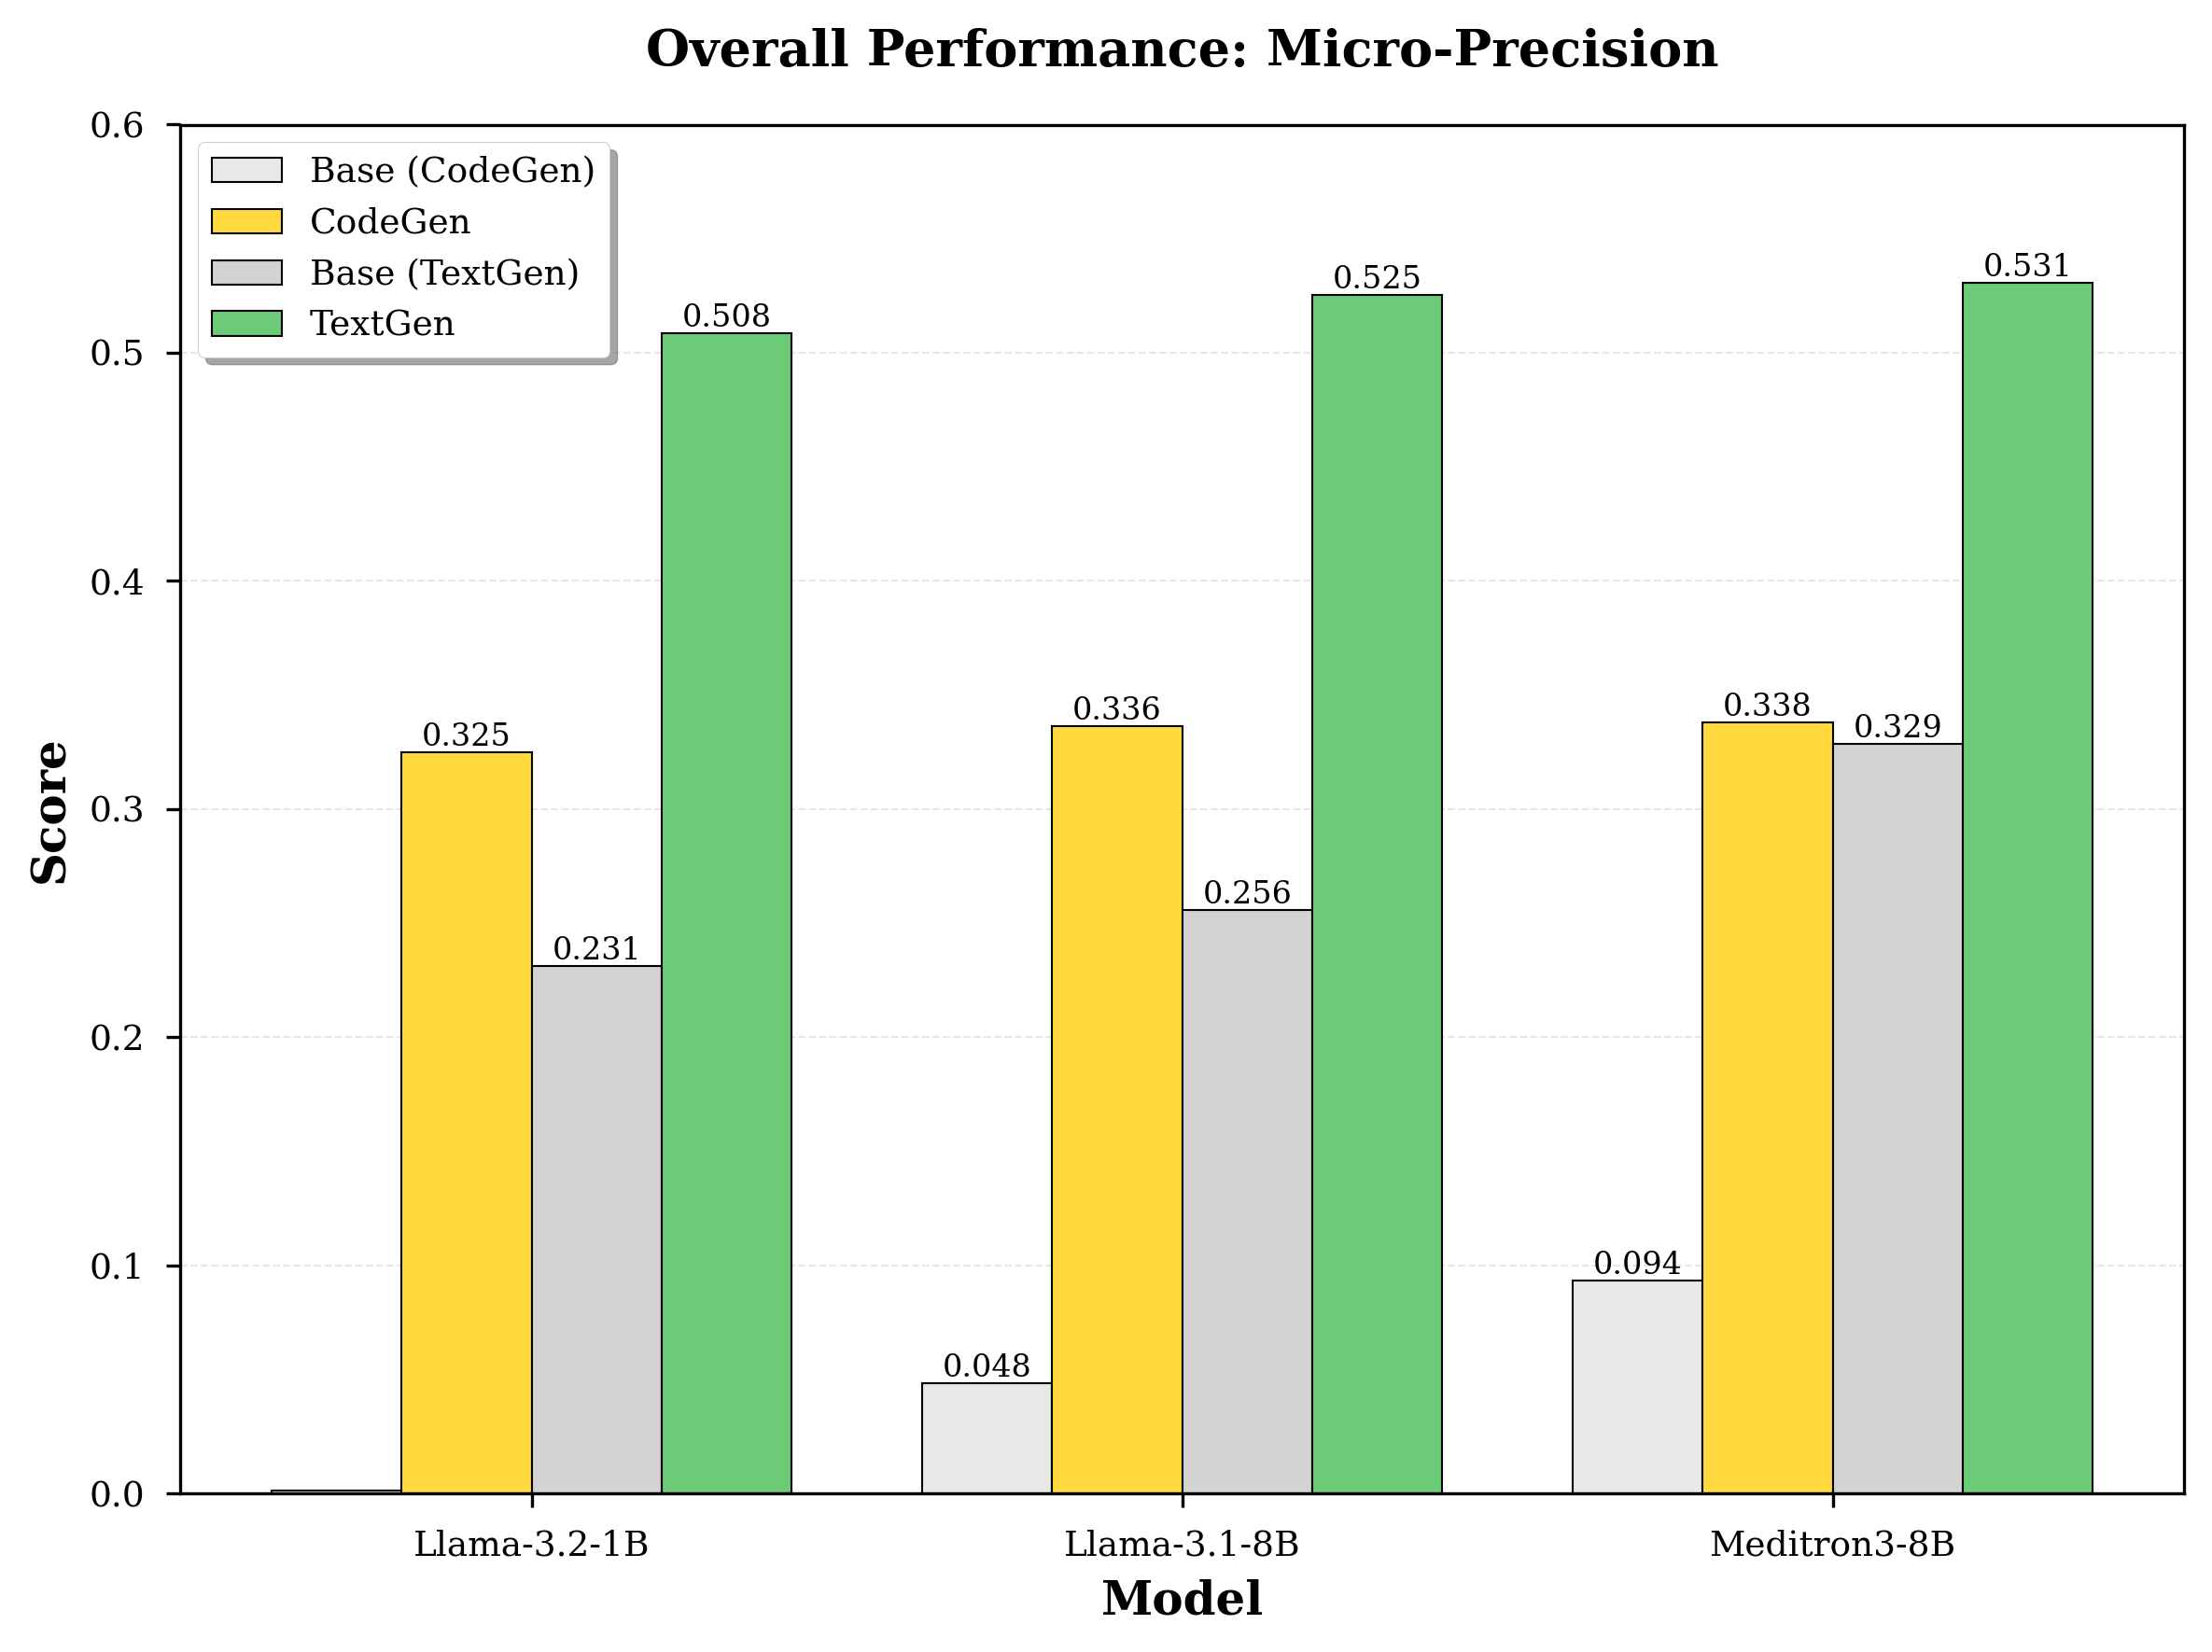
\includegraphics[width=\linewidth]{Images/Plots_thesis/overall_micro_precision.png}
%         \caption{Micro-Precision}
%         \label{fig:task1-flat-microP}
%     \end{subfigure}\hfill
%     \begin{subfigure}{0.32\textwidth}
%         \centering
%         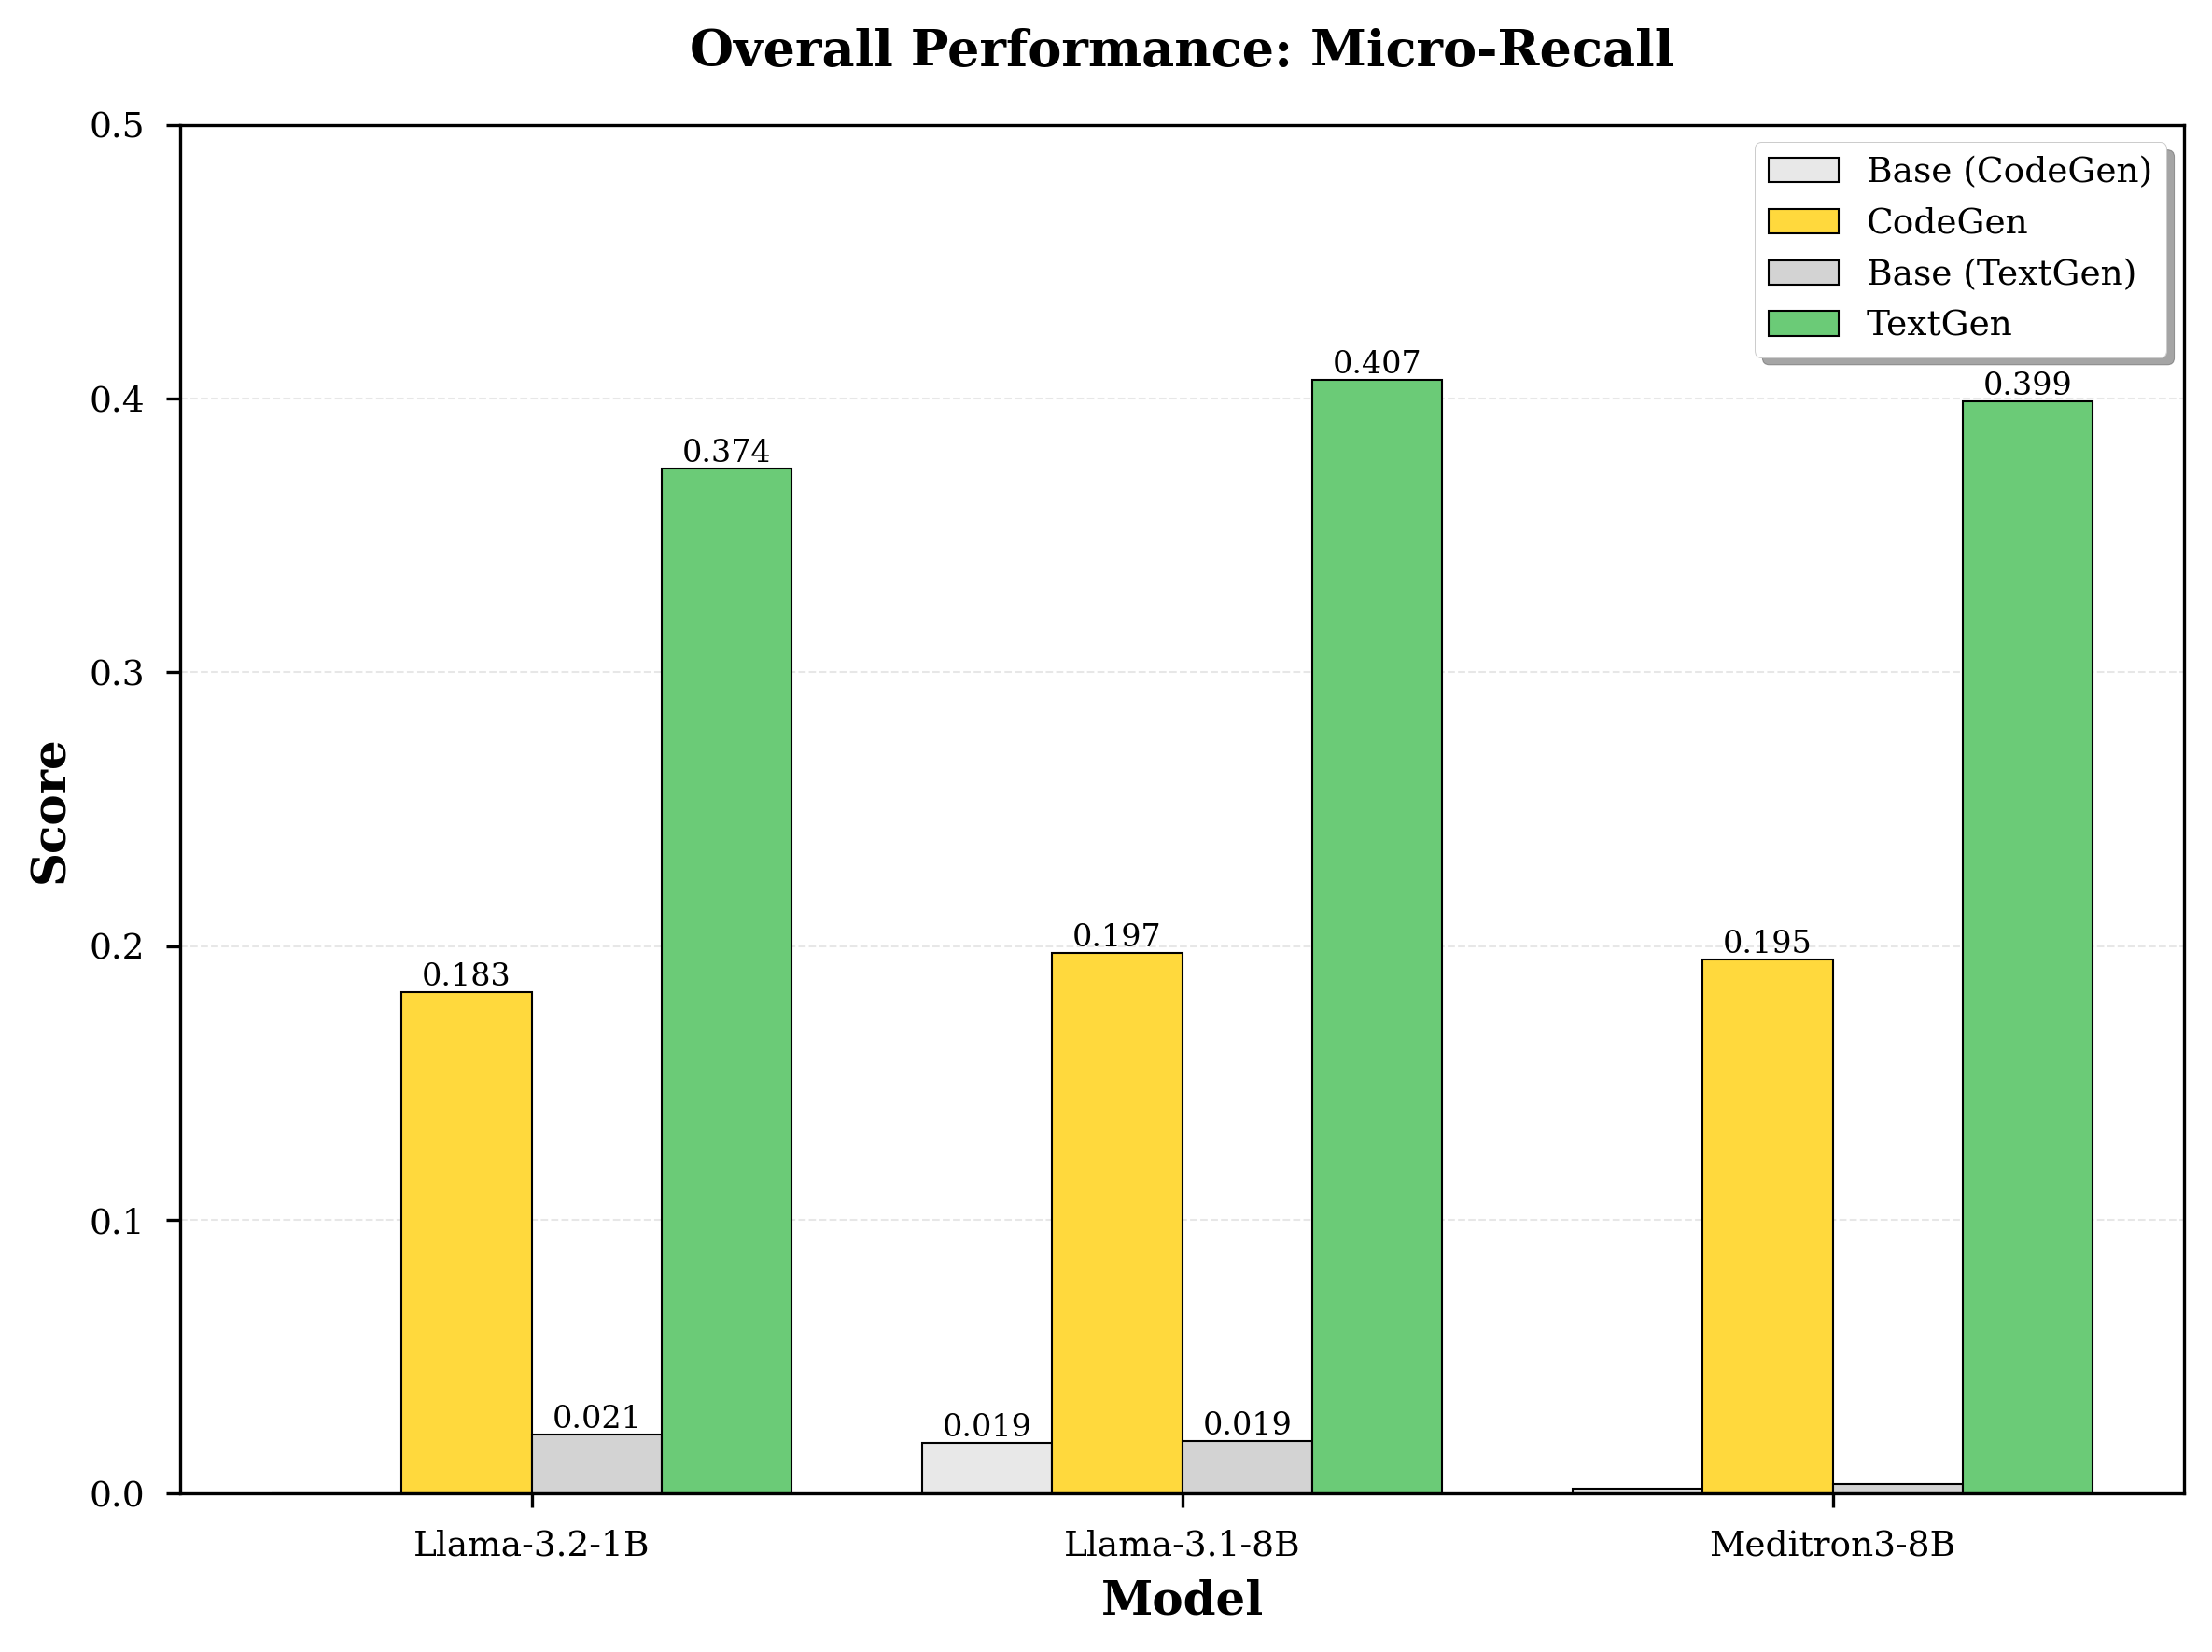
\includegraphics[width=\linewidth]{Images/Plots_thesis/overall_micro_recall.png}
%         \caption{Micro-Recall}
%         \label{fig:task1-flat-microR}
%     \end{subfigure}\hfill
%     \begin{subfigure}{0.32\textwidth}
%         \centering
%         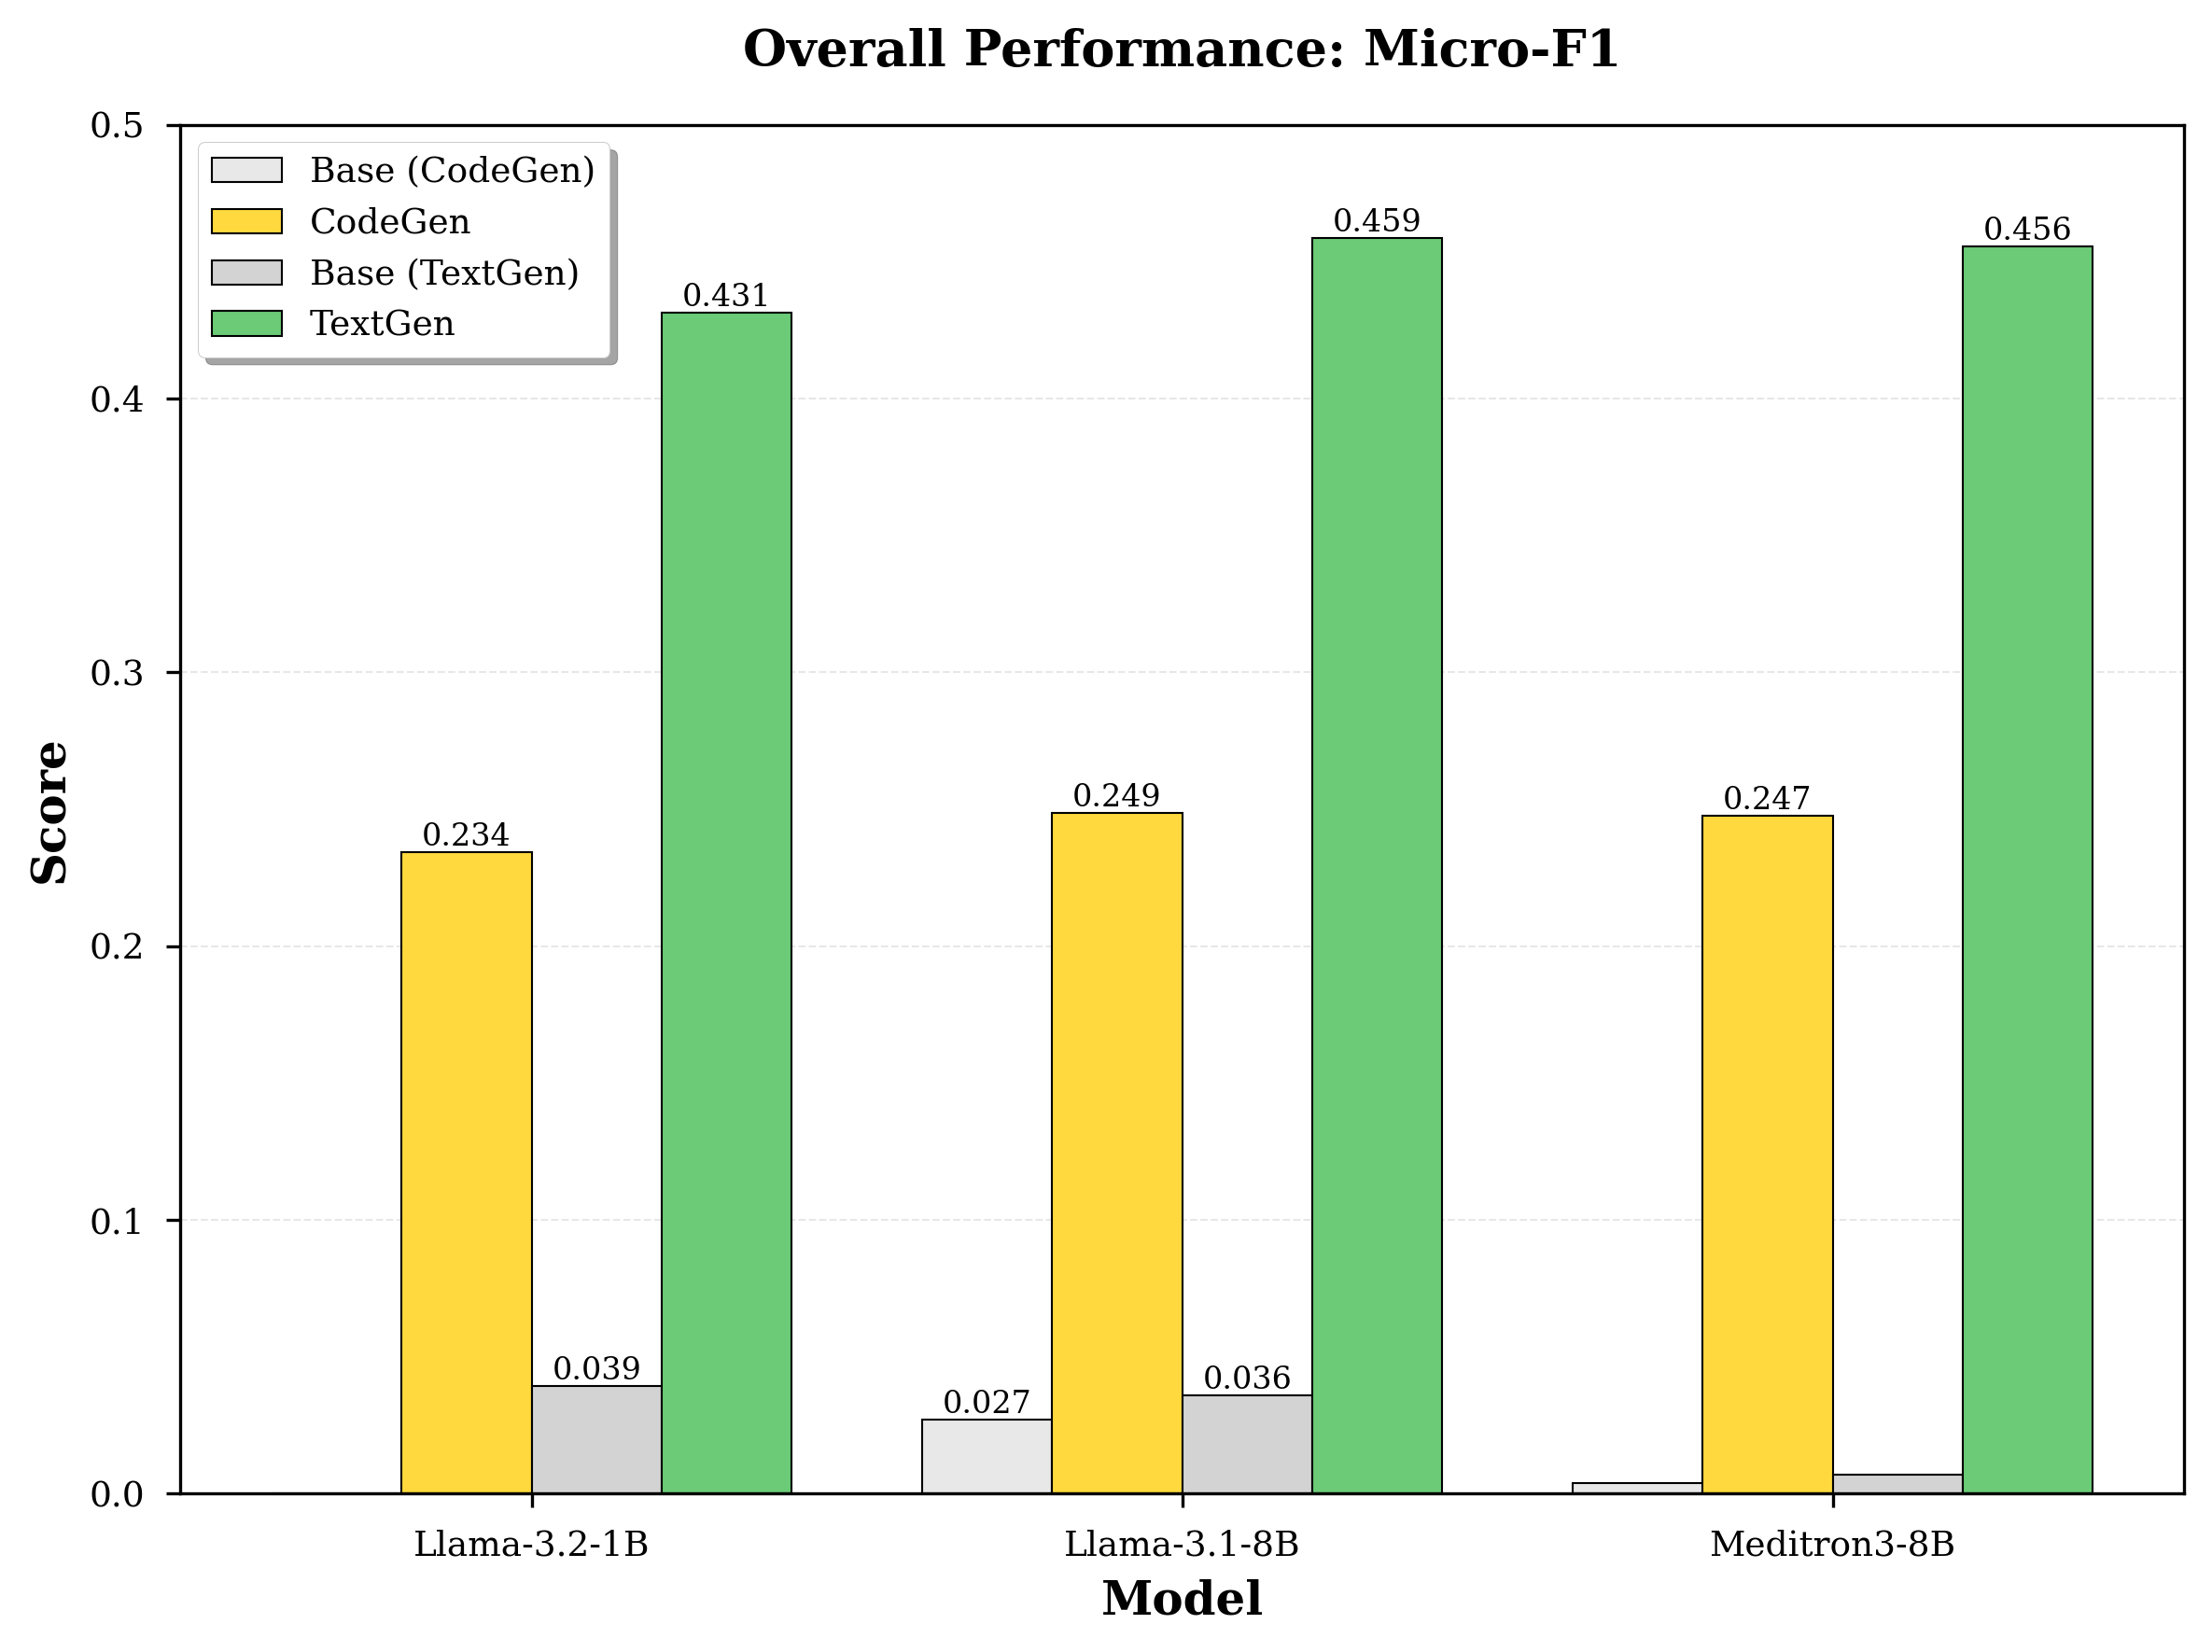
\includegraphics[width=\linewidth]{Images/Plots_thesis/overall_micro_f1.png}
%         \caption{Micro-F1}
%         \label{fig:task1-flat-microF1}
%     \end{subfigure}

%     \vspace{0.3cm}

%     % Bottom row: macro-averaged metrics
%     \begin{subfigure}{0.32\textwidth}
%         \centering
%         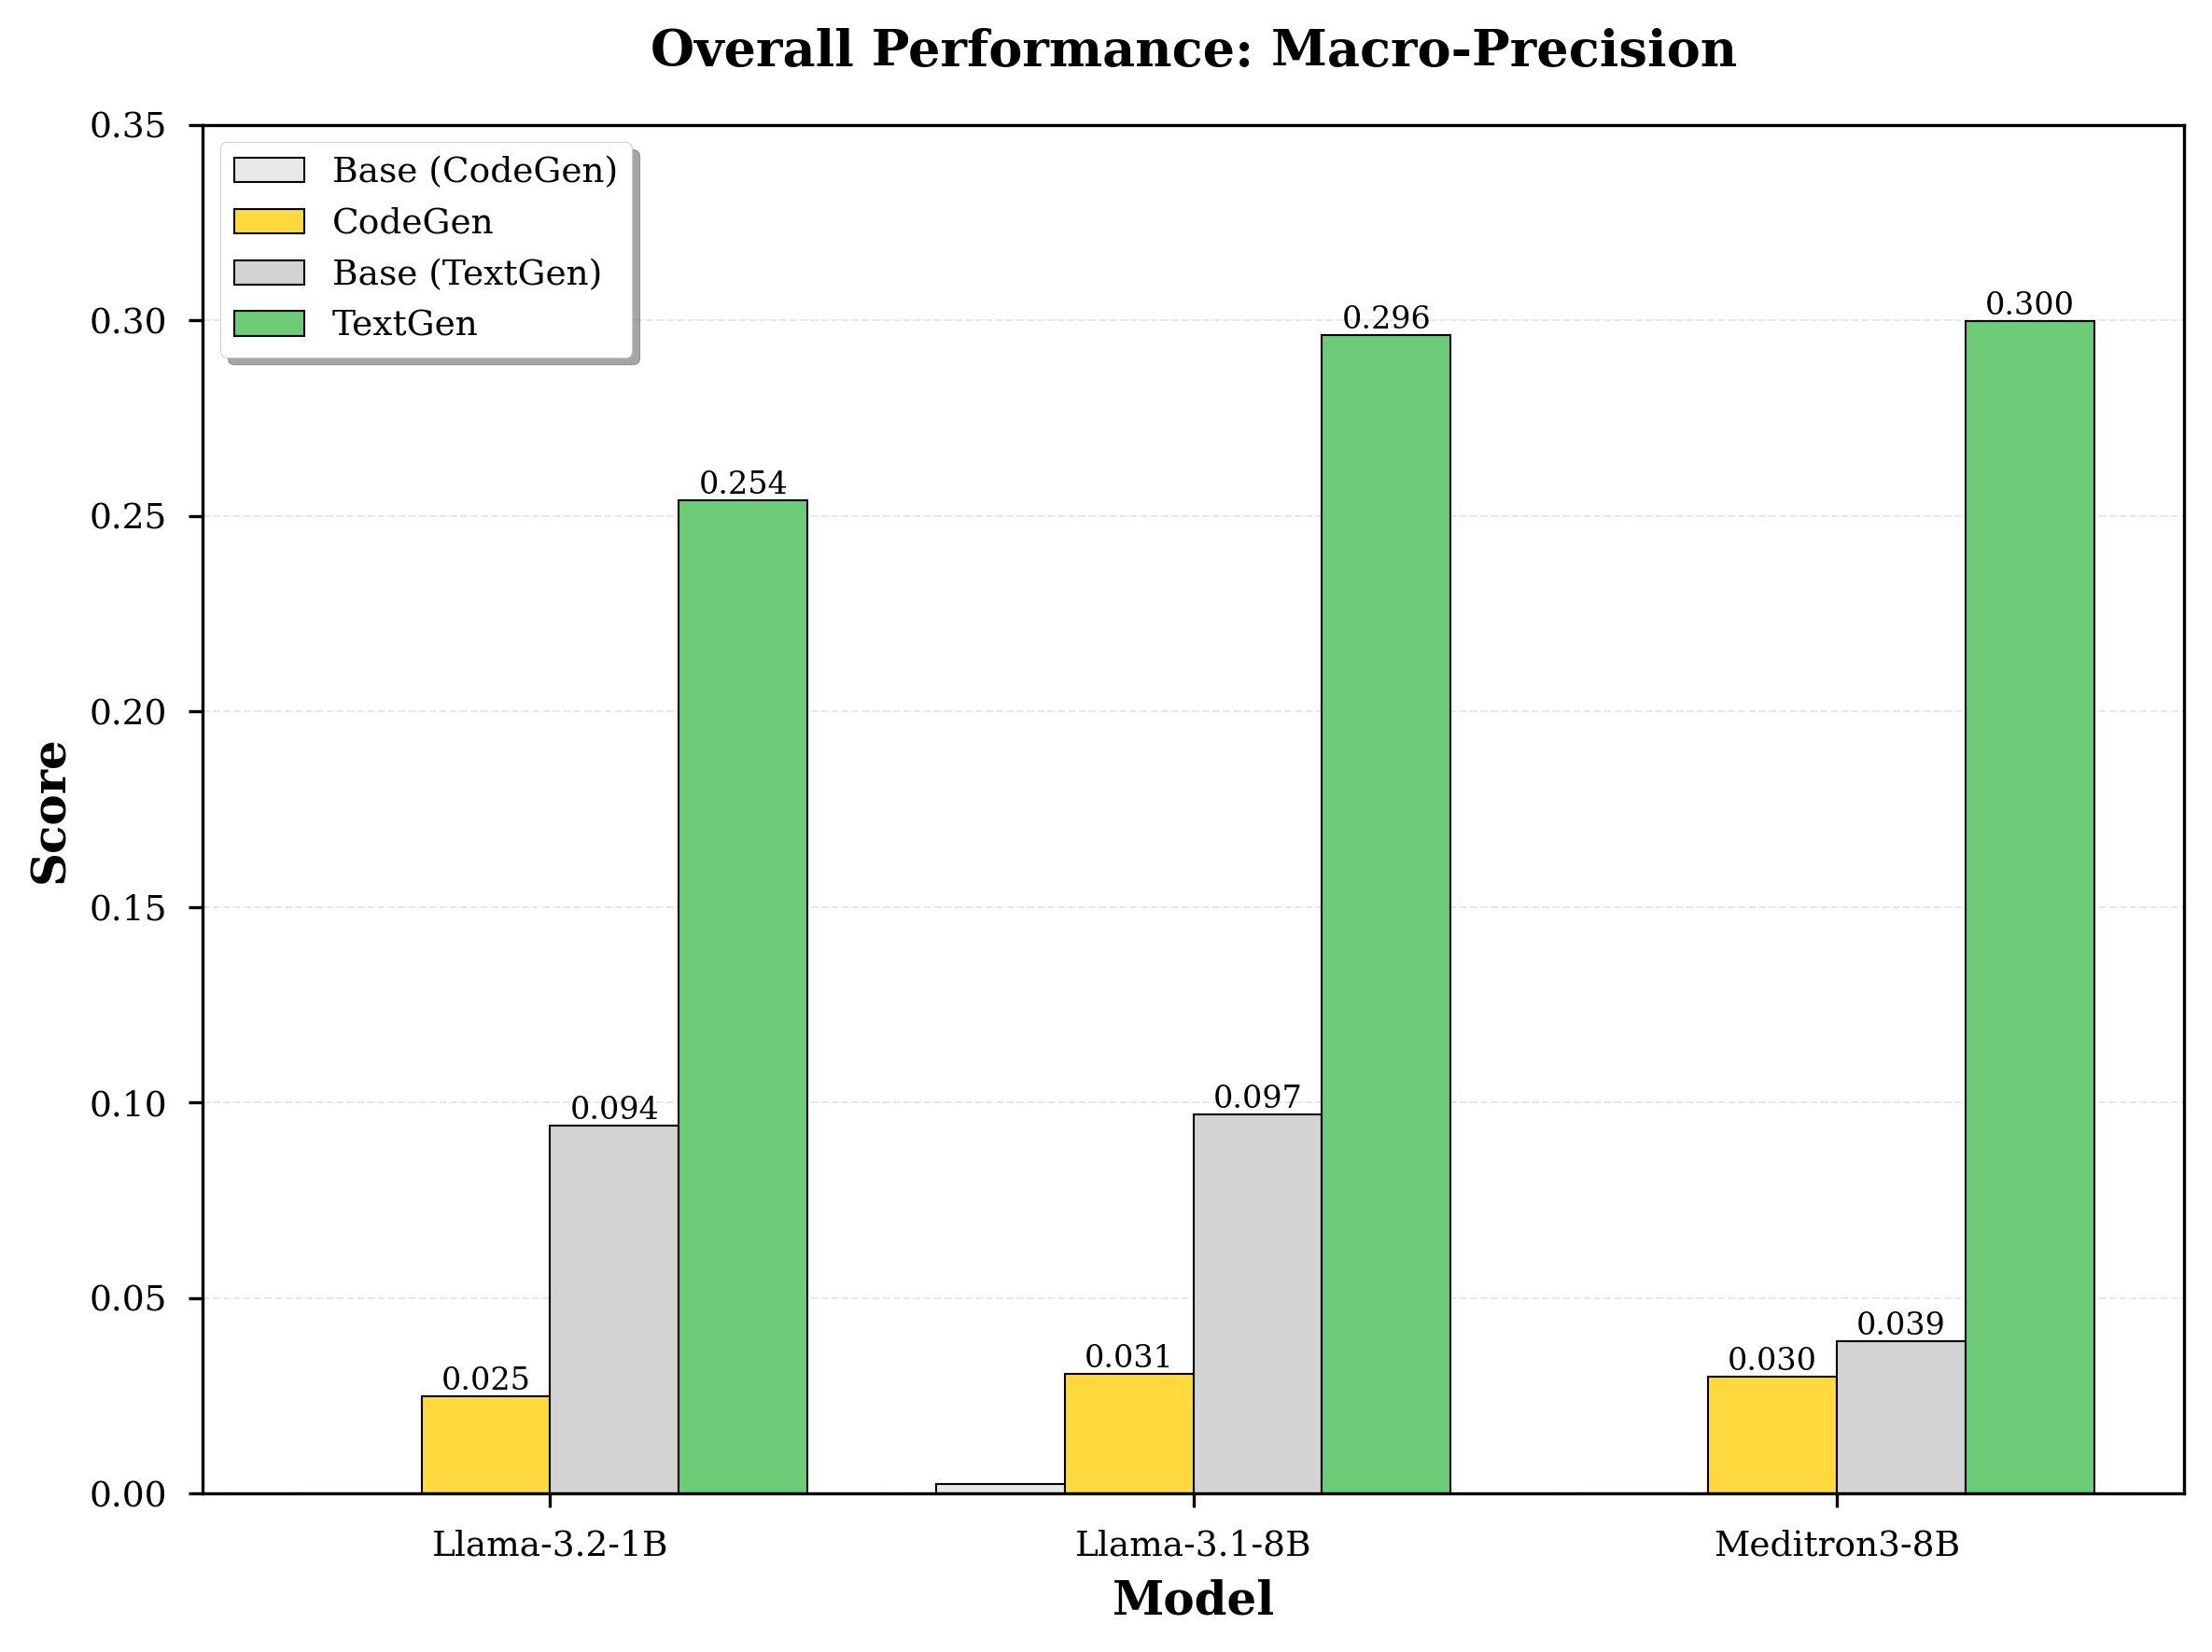
\includegraphics[width=\linewidth]{Images/Plots_thesis/overall_macro_precision.png}
%         \caption{Macro-Precision}
%         \label{fig:task1-flat-macroP}
%     \end{subfigure}\hfill
%     \begin{subfigure}{0.32\textwidth}
%         \centering
%         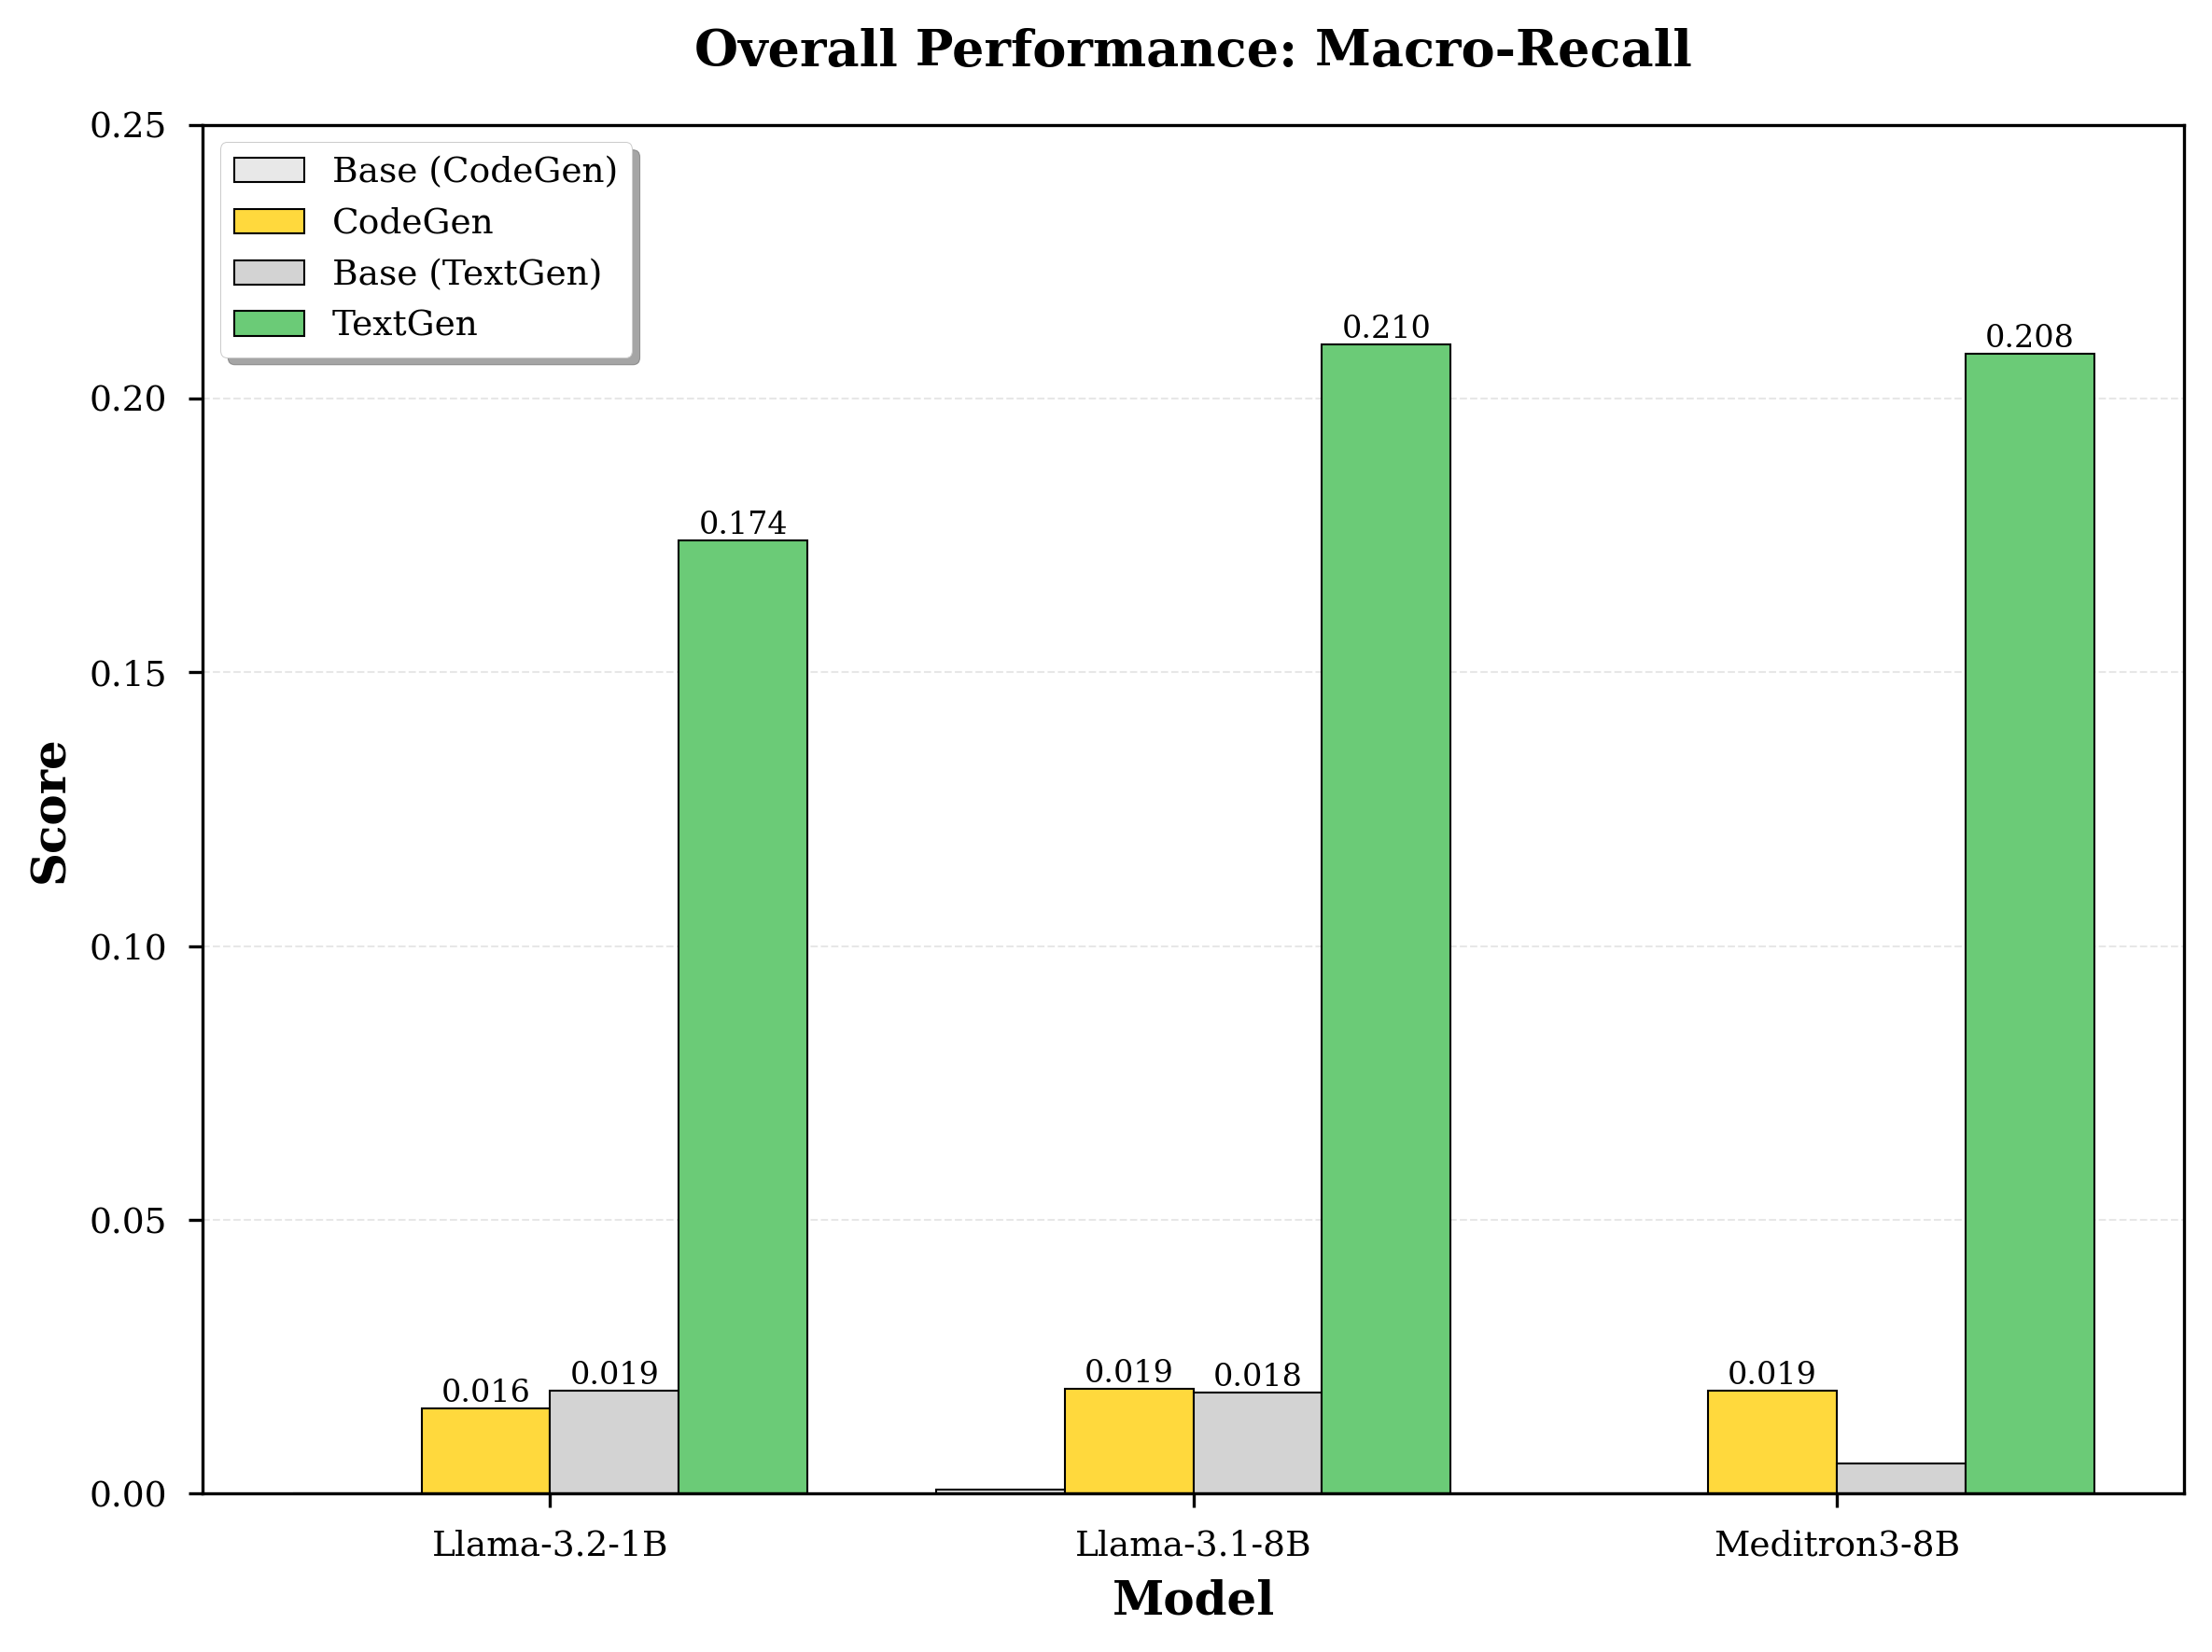
\includegraphics[width=\linewidth]{Images/Plots_thesis/overall_macro_recall.png}
%         \caption{Macro-Recall}
%         \label{fig:task1-flat-macroR}
%     \end{subfigure}\hfill
%     \begin{subfigure}{0.32\textwidth}
%         \centering
%         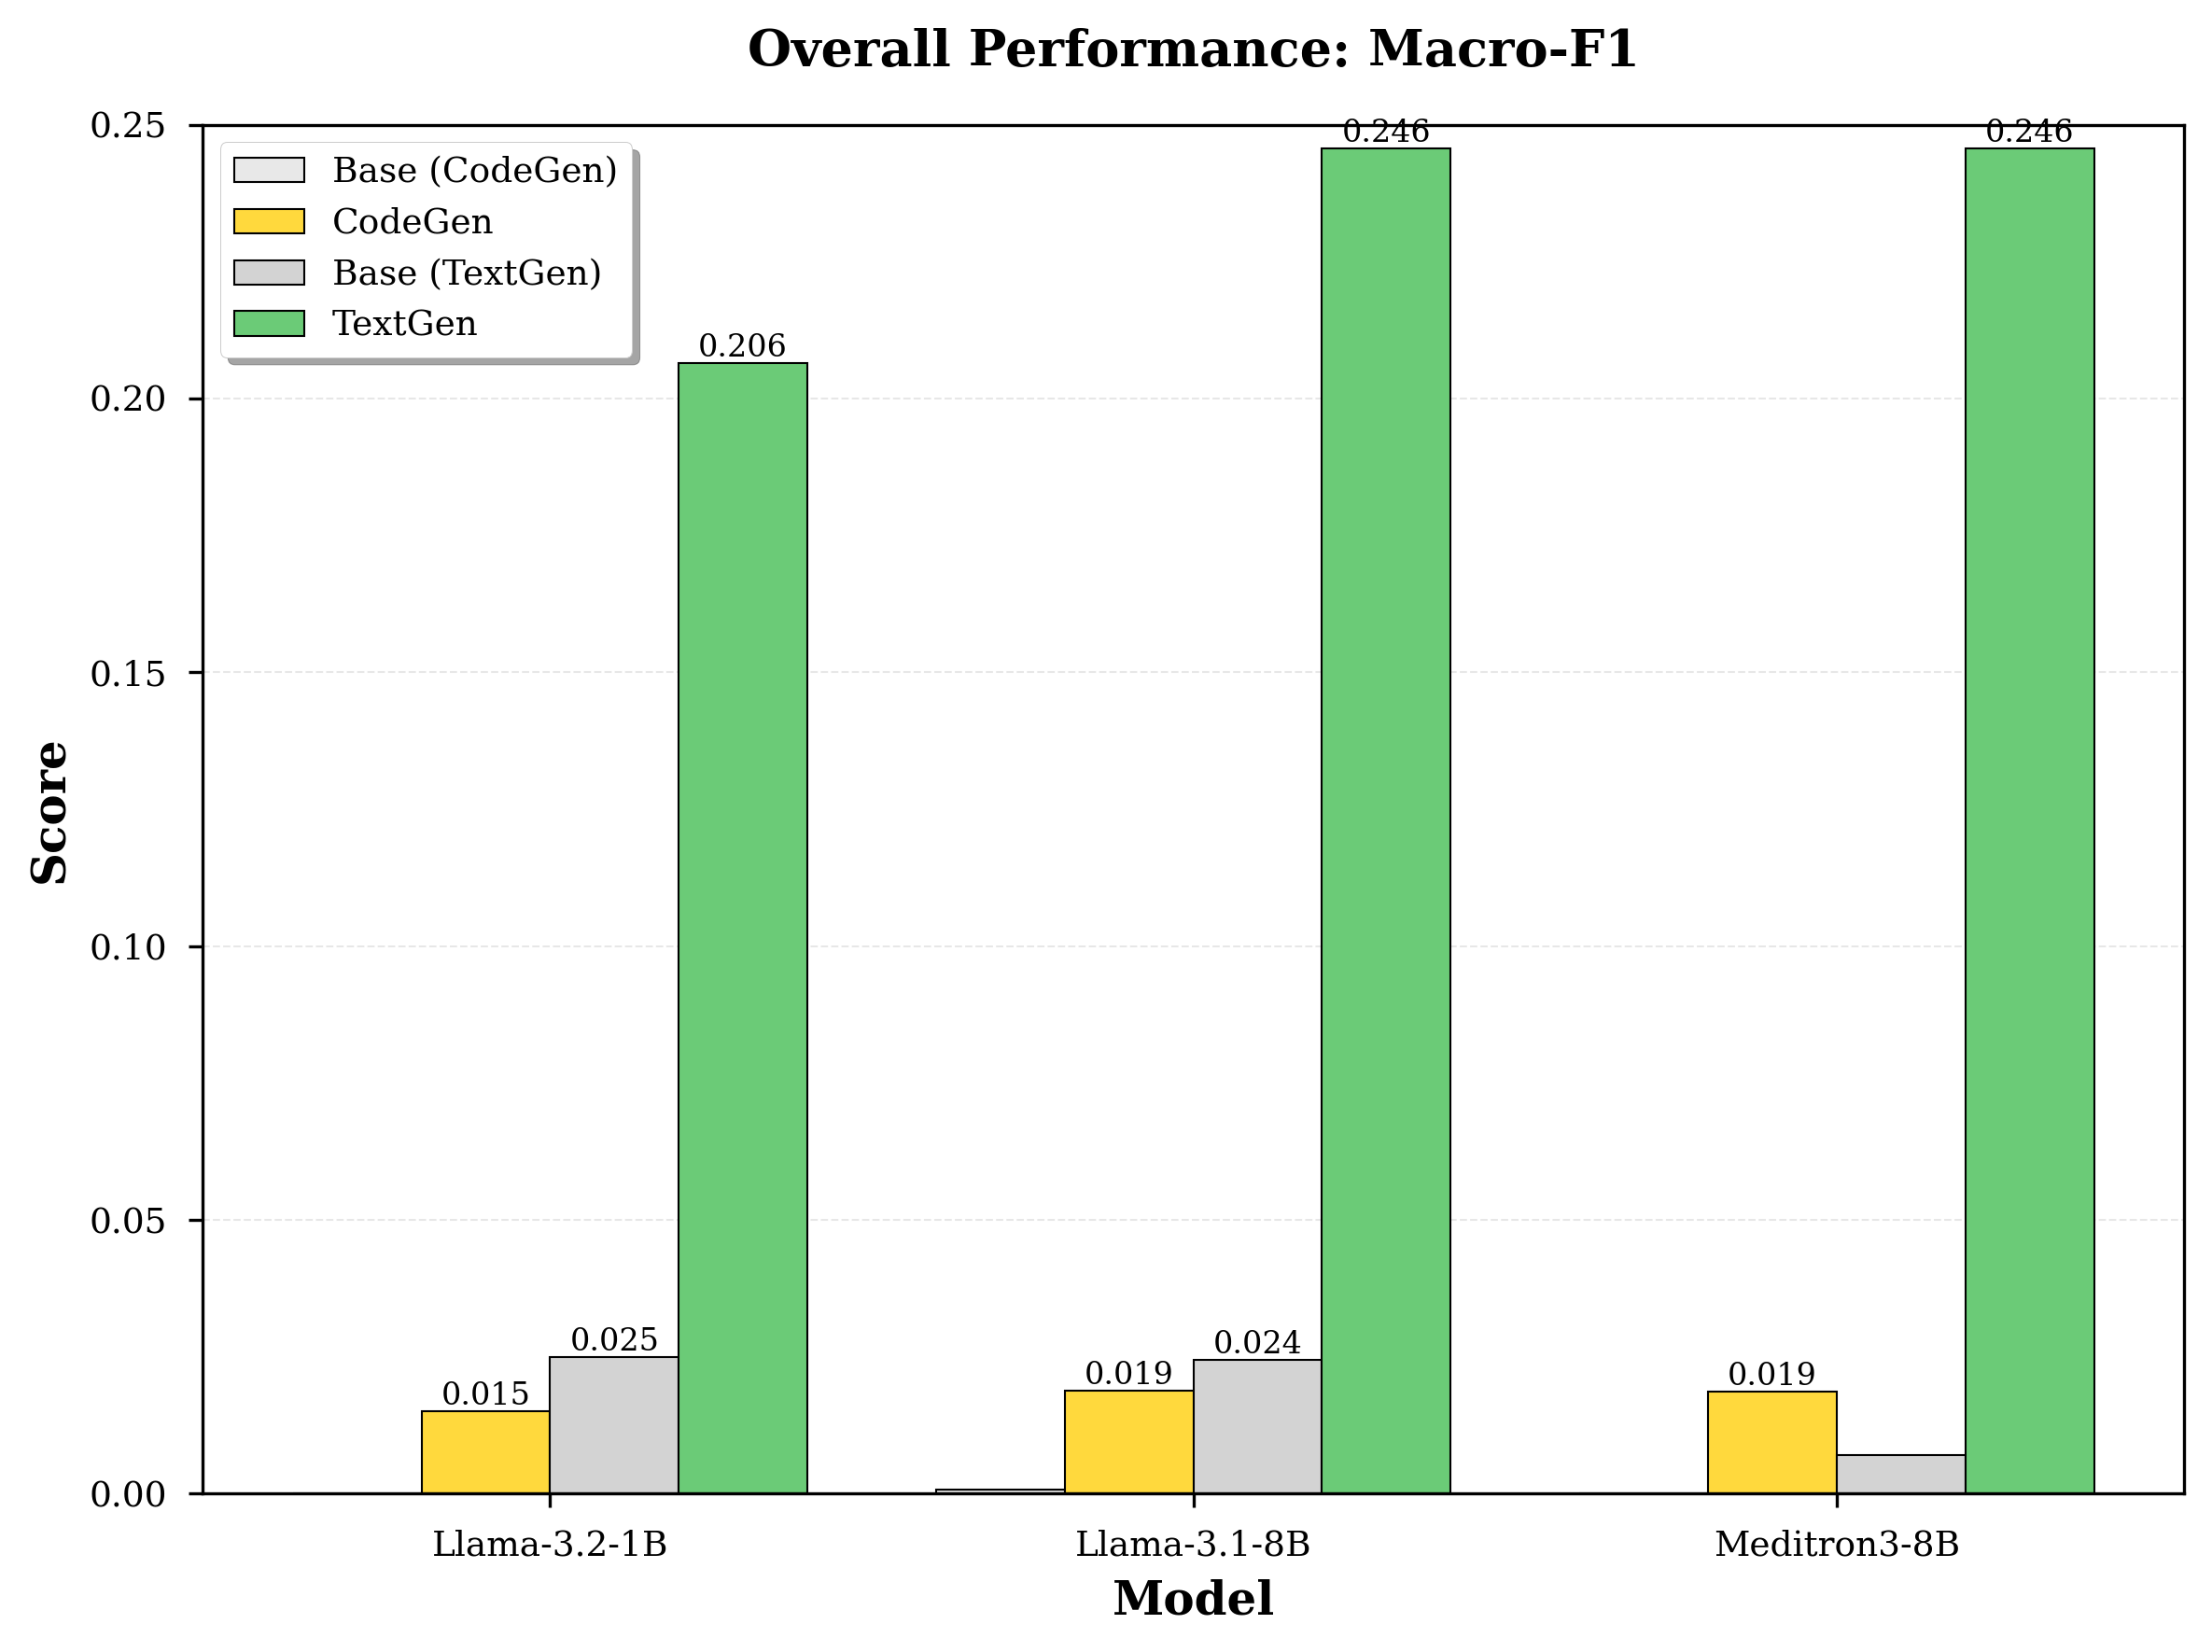
\includegraphics[width=\linewidth]{Images/Plots_thesis/overall_macro_f1.png}
%         \caption{Macro-F1}
%         \label{fig:task1-flat-macroF1}
%     \end{subfigure}

%     \caption{Task~1: flat (full-code) evaluation. Micro- and macro-averaged precision, recall, and F1 for \textbf{Base} (raw backbones), \textbf{CodeGen} (fine-tuned direct ICD-9 generation), and \textbf{TextGen} (fine-tuned diagnosis-term generation + semantic mapping) across all backbones.}
%     \label{fig:task1-flat-metrics}
% \end{figure}

% Overall, Table~\ref{tab:task1-all-methods-flat} and Figure~\ref{fig:task1-flat-metrics} establish a clear ranking:
% \[
% \text{Base} \;\ll\; \text{CodeGen} \;<\; \text{TextGen},
% \]
% with stronger performance for 8B backbones than 1B. These findings justify using \textbf{TextGen} as the default pipeline for subsequent knowledge-augmentation experiments.

% % ============================================================
% \subsection{Hierarchical Evaluation at the Parent-Code Level}
% \label{subsec:results-task1-hierarchical}

% Flat ICD-9 evaluation assigns full penalty to any mismatch at the exact code level, even if the predicted code falls under the correct diagnostic family. To quantify clinically meaningful ``near misses'', we compute \emph{parent-level} metrics (Section~\ref{subsec:hierarchical-metrics}), where codes are collapsed to their three-digit parent categories.

% Table~\ref{tab:task1-parent-metrics} shows a consistent increase in F1 relative to full-code evaluation, indicating that many errors occur within the correct disease family (e.g., predicting a related subtype rather than a completely unrelated diagnosis). TextGen retains a clear advantage at the parent level, implying its gains reflect improved clinical alignment rather than merely better formatting.

% \begin{table}[t]
%     \centering
%     \caption{Task~1 hierarchical evaluation at the ICD-9 parent (three-digit) level. Metrics computed after collapsing codes to parent categories (test set).}
%     \label{tab:task1-parent-metrics}
%     \begin{tabular}{llcc}
%         \toprule
%         \textbf{Backbone} & \textbf{Method} &
%         \textbf{Parent micro-F1} &
%         \textbf{Parent macro-F1} \\
%         \midrule
%         \multirow{4}{*}{Llama-3.2-1B} 
%             & Base (no FT) - Direct codes   & 0.0014 & 0.0007 \\
%             & CodeGen        & 0.4687 & 0.2572 \\
%             & Base (no FT) - Free Text  & 0.0677 & 0.0387  \\
%             & TextGen        & \textbf{0.4800} & \textbf{0.2732} \\
%         \midrule
%         \multirow{4}{*}{Llama-3.1-8B} 
%             & Base (no FT) - Direct codes   & 0.0953 & 0.0281 \\
%             & CodeGen        & 0.4814 & 0.2973 \\
%             & Base (no FT) - Free Text  & 0.0618 & 0.0378  \\
%             & TextGen        & \textbf{0.5388} & \textbf{0.3459} \\
%         \midrule
%         \multirow{4}{*}{Meditron-8B} 
%             & Base (no FT) - Direct codes   & 0.0083 & 0.0015 \\
%             & CodeGen        & 0.4771 & 0.2935 \\
%             & Base (no FT) - Free Text  & 0.0135 & 0.0111  \\
%             & TextGen        & \textbf{0.5364} & \textbf{0.3418} \\
%         \bottomrule
%     \end{tabular}
% \end{table}

% % --- KEEP THESE IMAGES EXACTLY (as requested) ---
% \begin{figure}[t]
%     \centering
%     % Top row: micro-averaged parent metrics
%     \begin{subfigure}{0.32\textwidth}
%         \centering
%         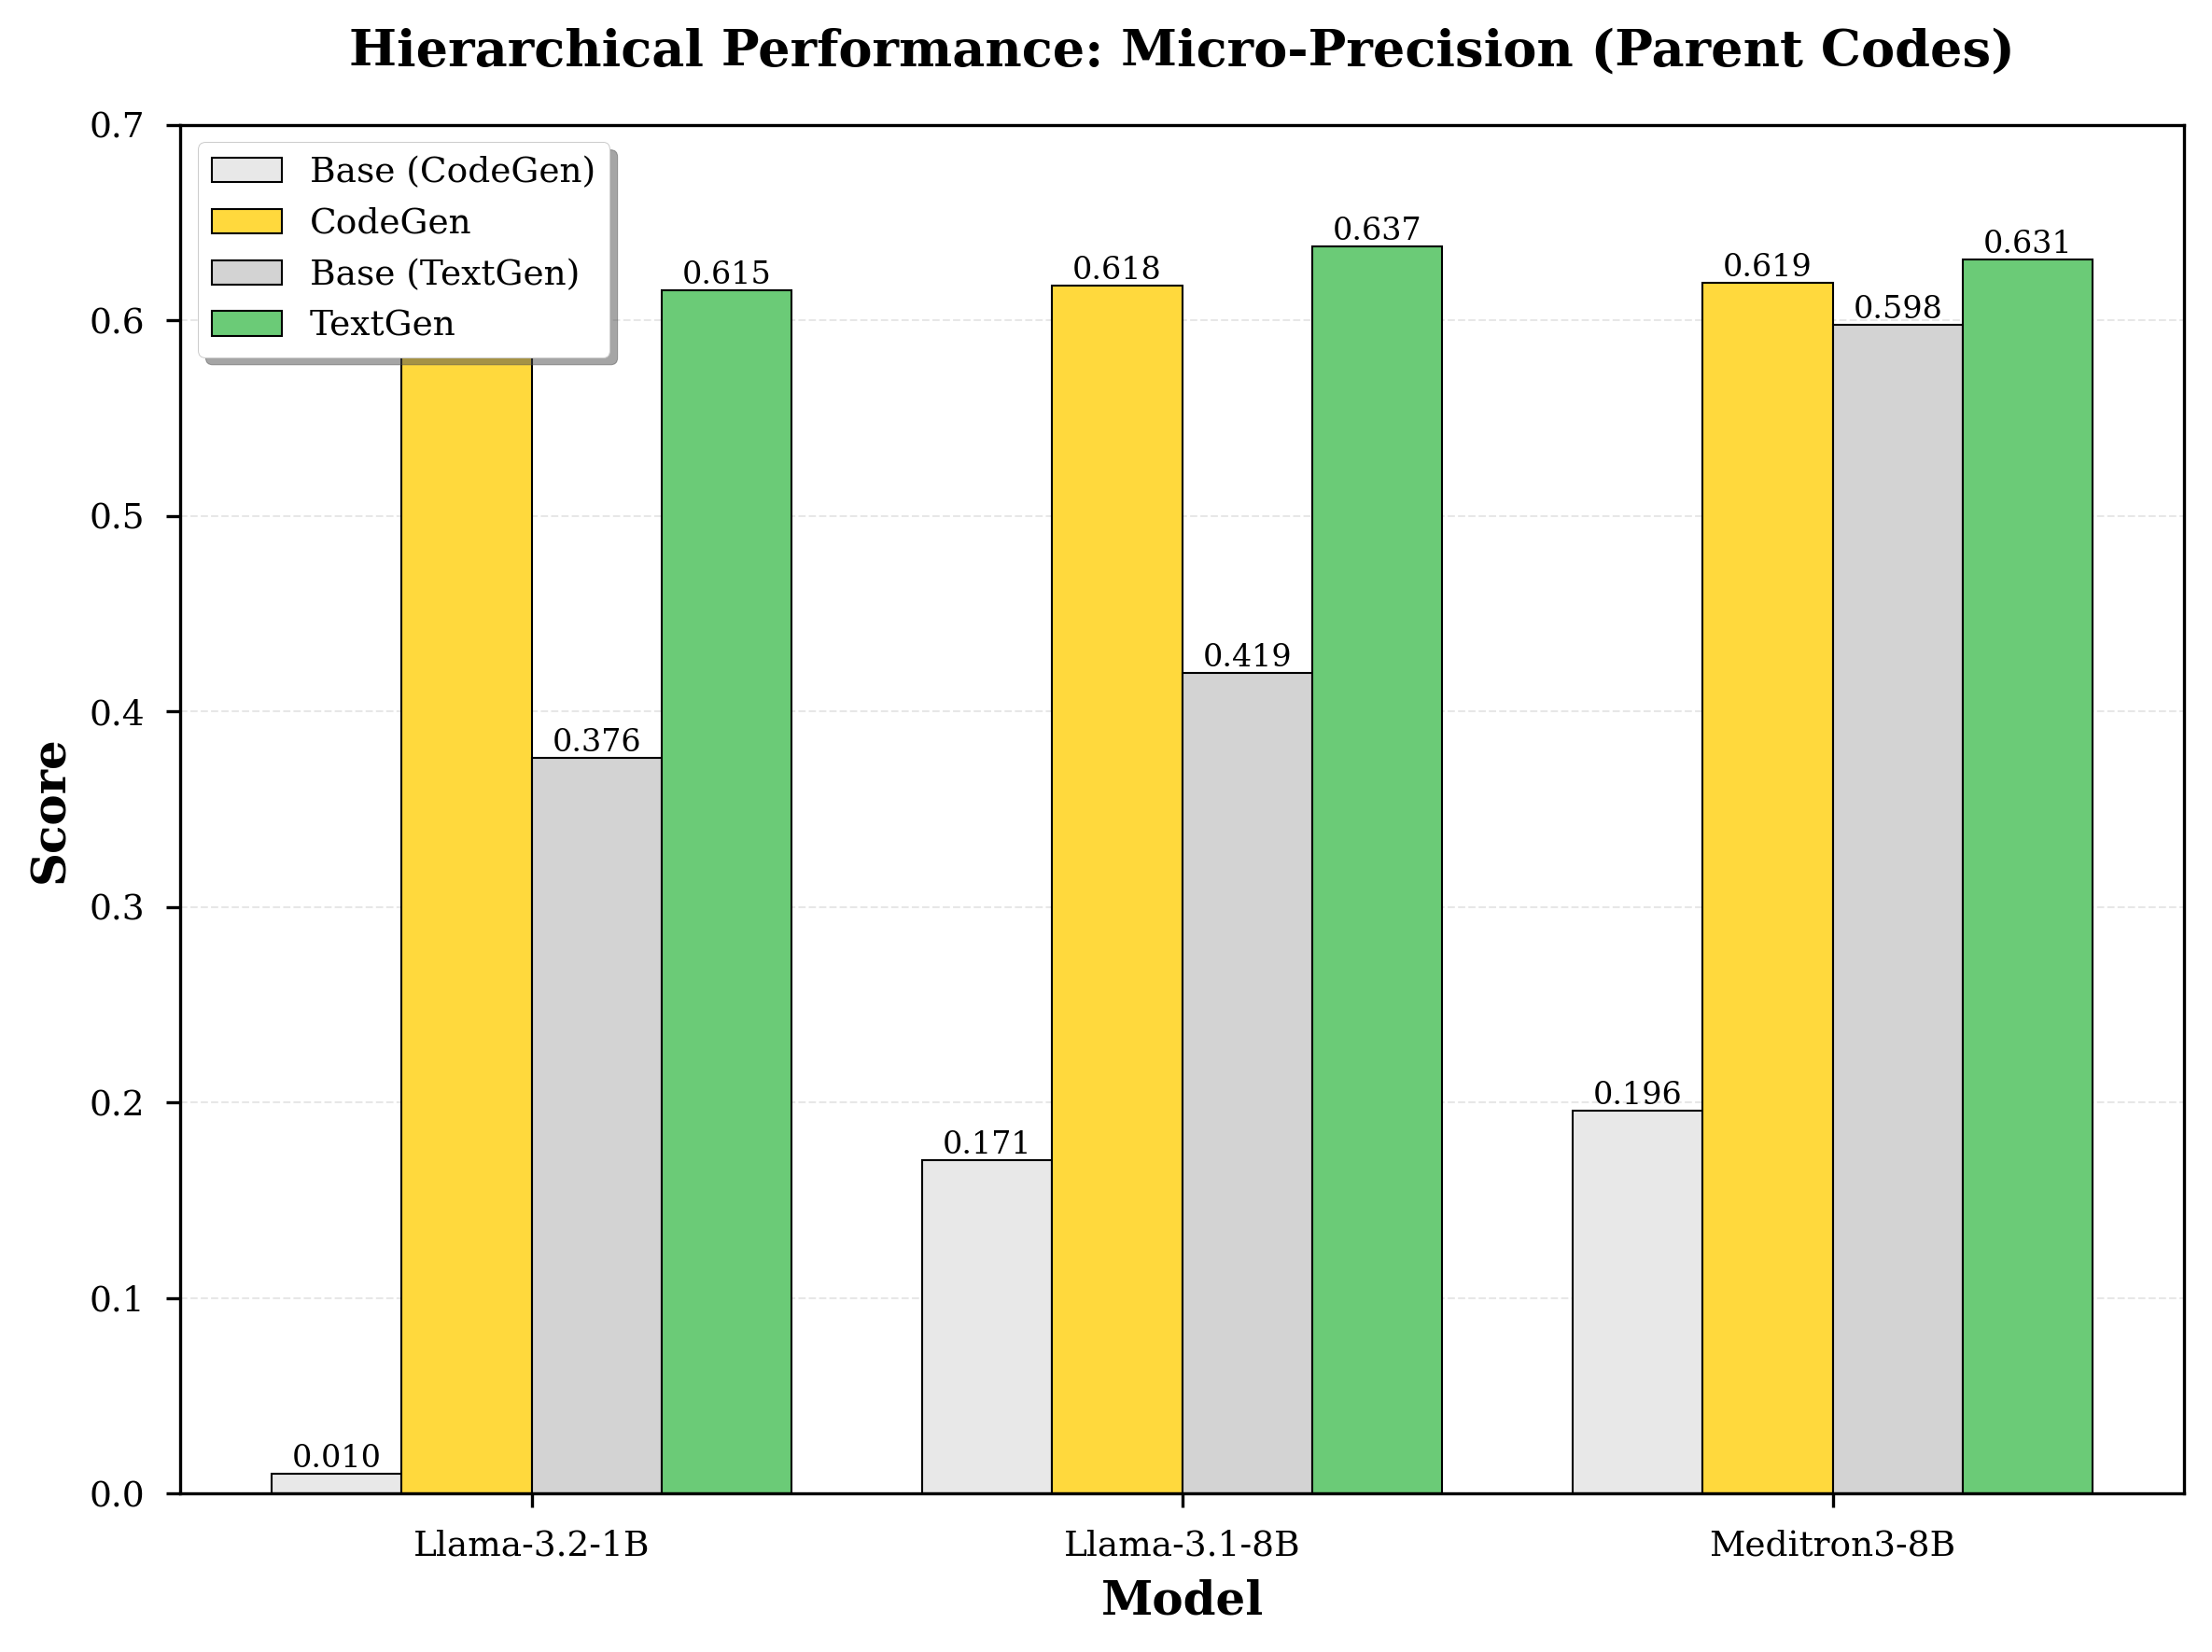
\includegraphics[width=\linewidth]{Images/Plots_thesis/parent_micro_precision.png}
%         \caption{Parent micro-Precision}
%         \label{fig:task1-parent-microP}
%     \end{subfigure}\hfill
%     \begin{subfigure}{0.32\textwidth}
%         \centering
%         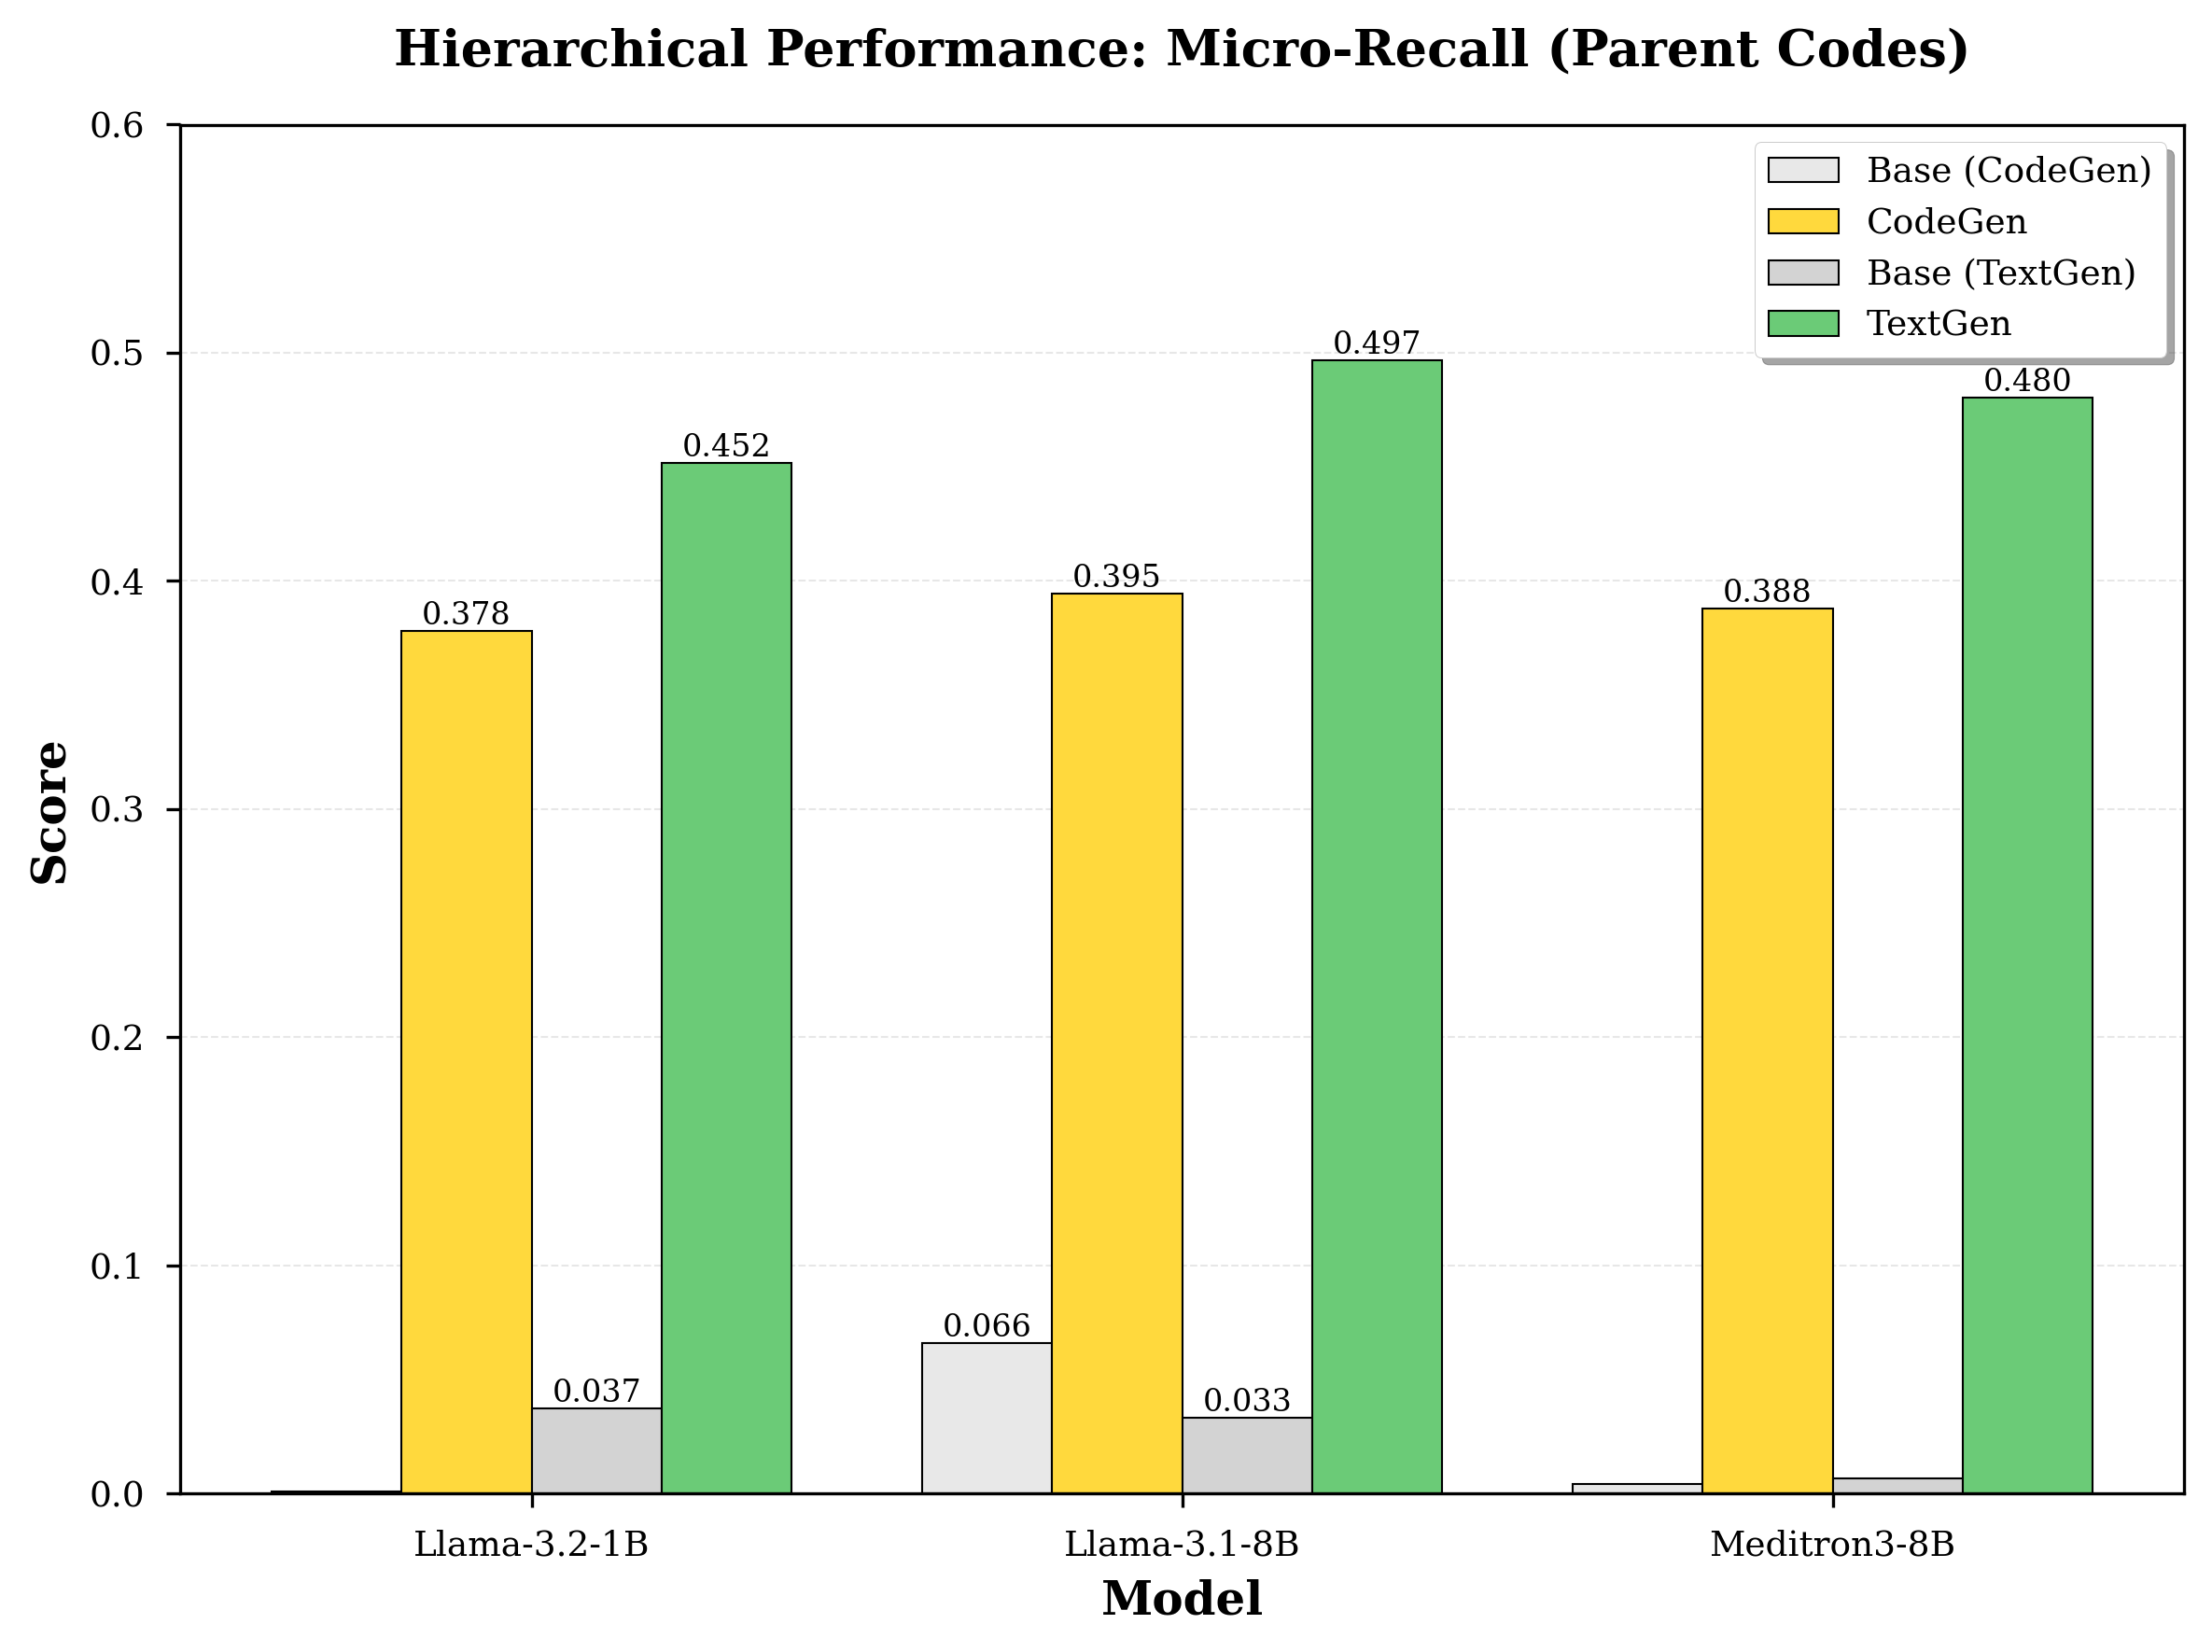
\includegraphics[width=\linewidth]{Images/Plots_thesis/parent_micro_recall.png}
%         \caption{Parent micro-Recall}
%         \label{fig:task1-parent-microR}
%     \end{subfigure}\hfill
%     \begin{subfigure}{0.32\textwidth}
%         \centering
%         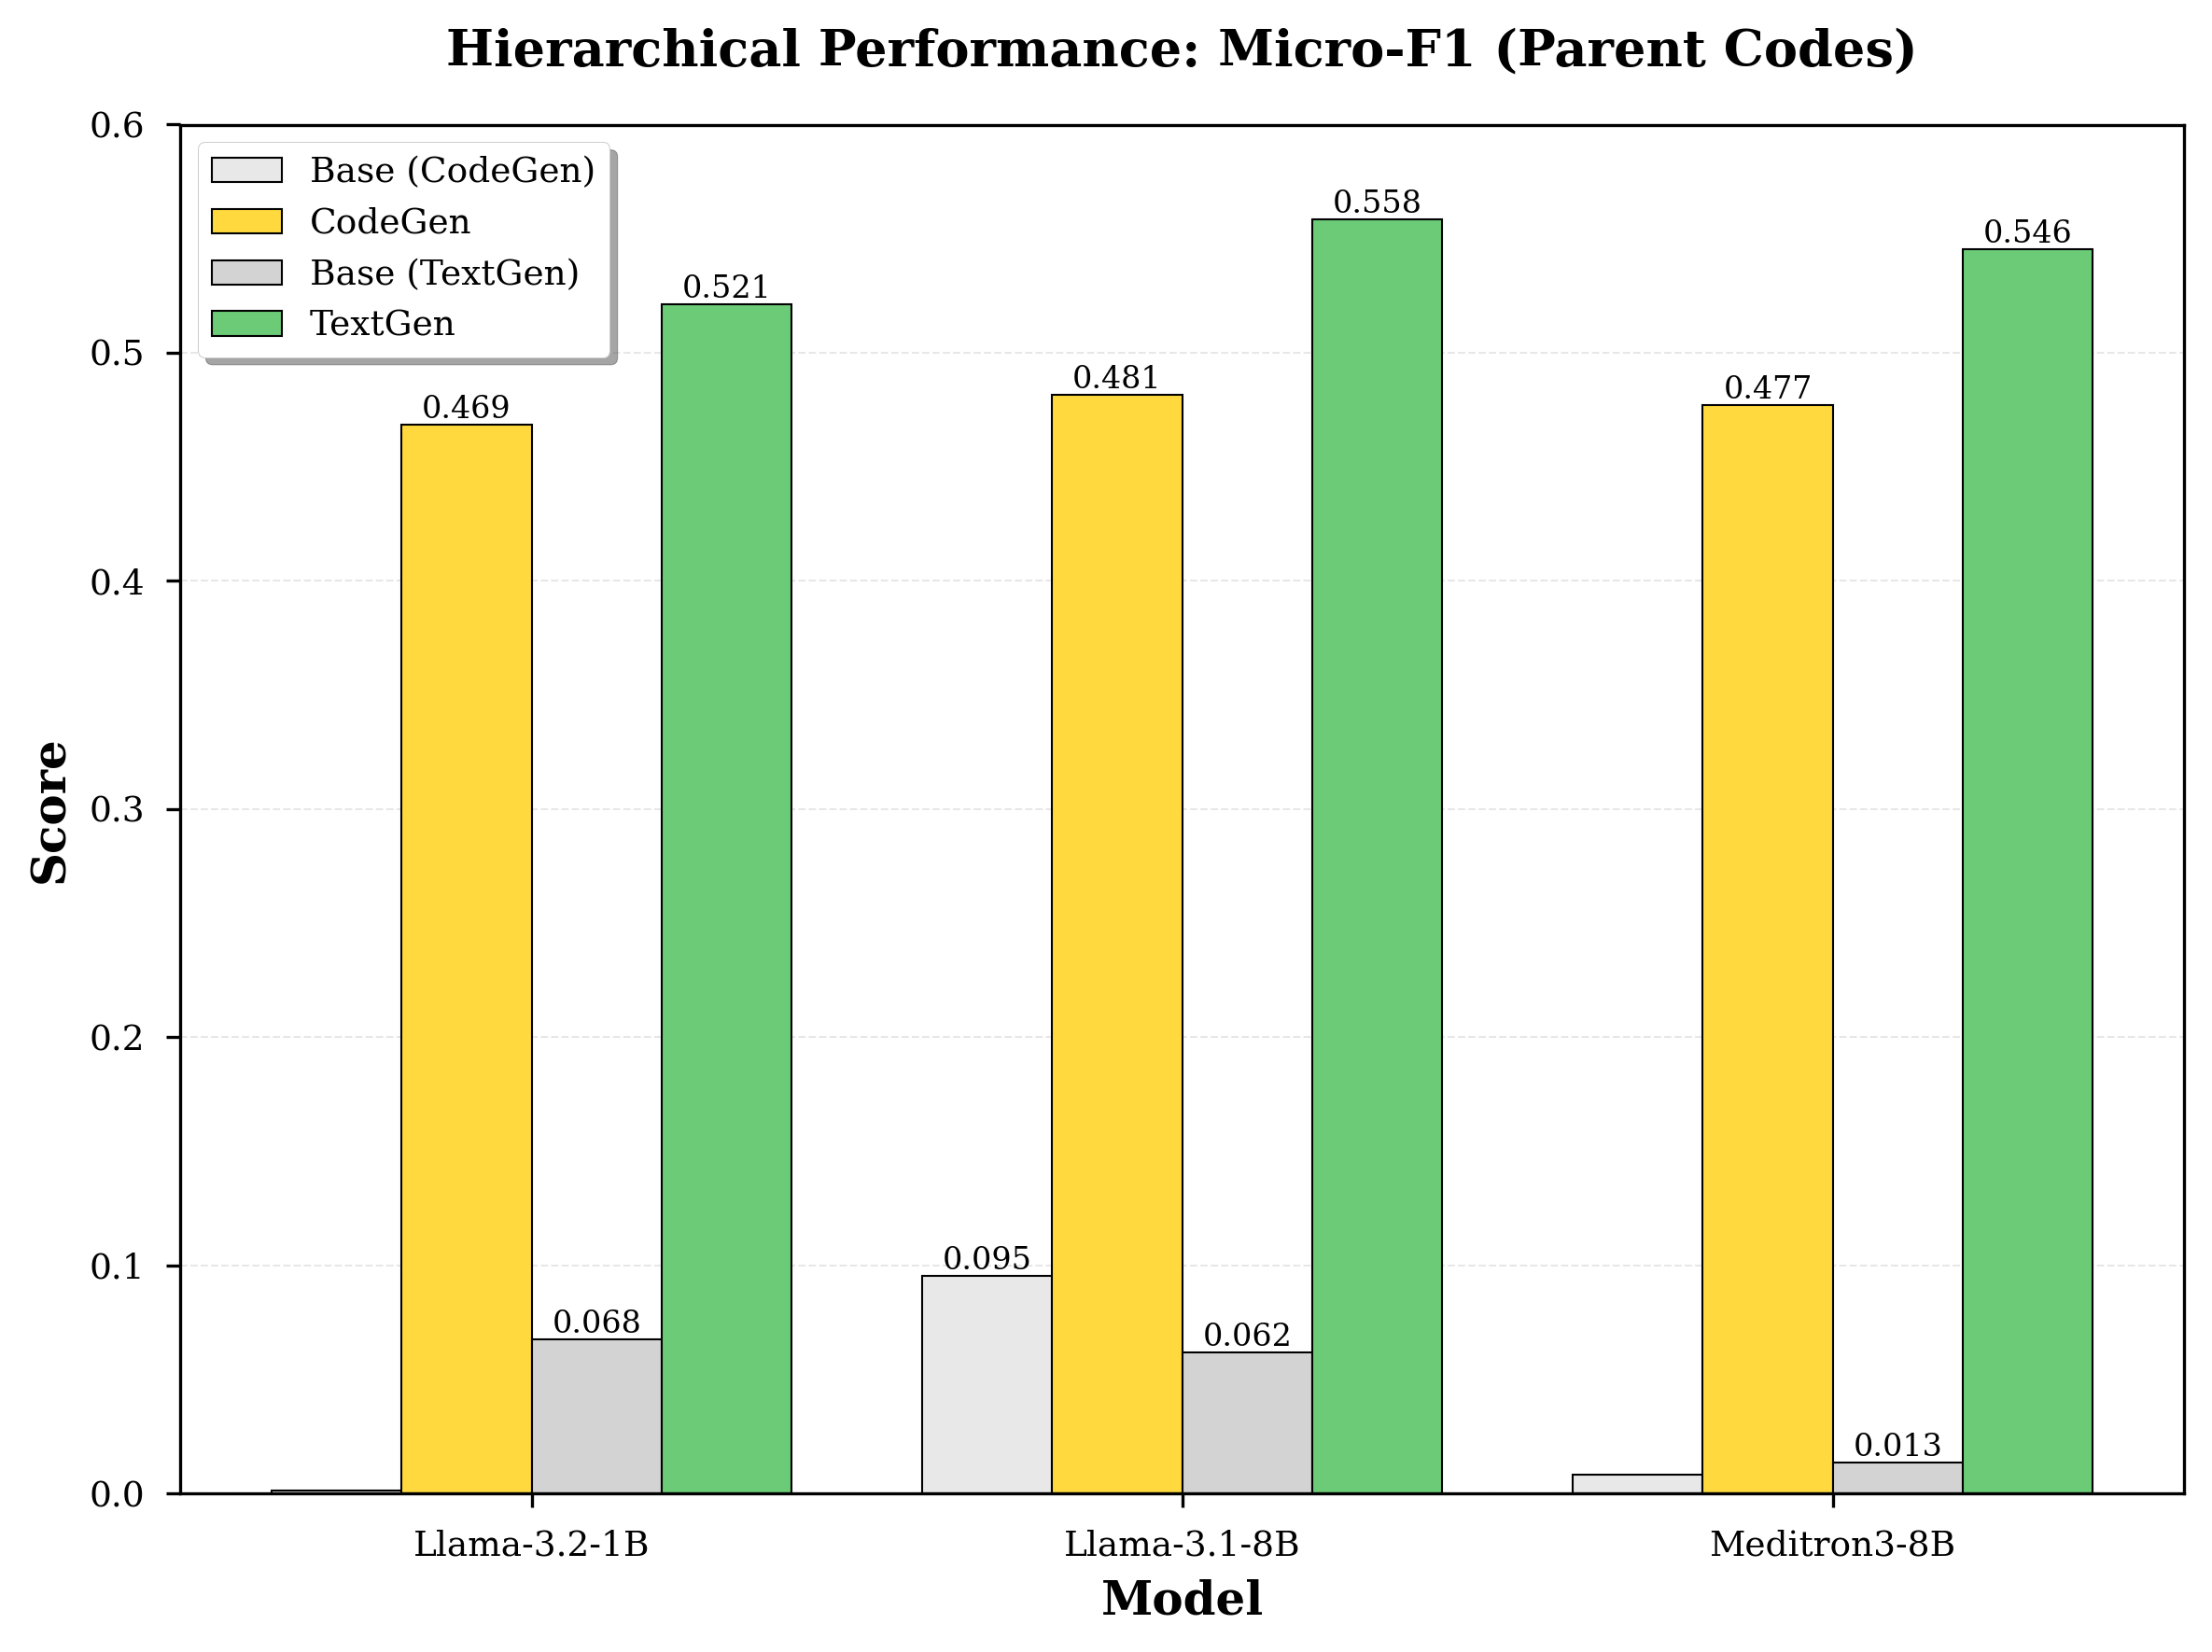
\includegraphics[width=\linewidth]{Images/Plots_thesis/parent_micro_f1.png}
%         \caption{Parent micro-F1}
%         \label{fig:task1-parent-microF1}
%     \end{subfigure}

%     \vspace{0.3cm}

%     % Bottom row: macro-averaged parent metrics
%     \begin{subfigure}{0.32\textwidth}
%         \centering
%         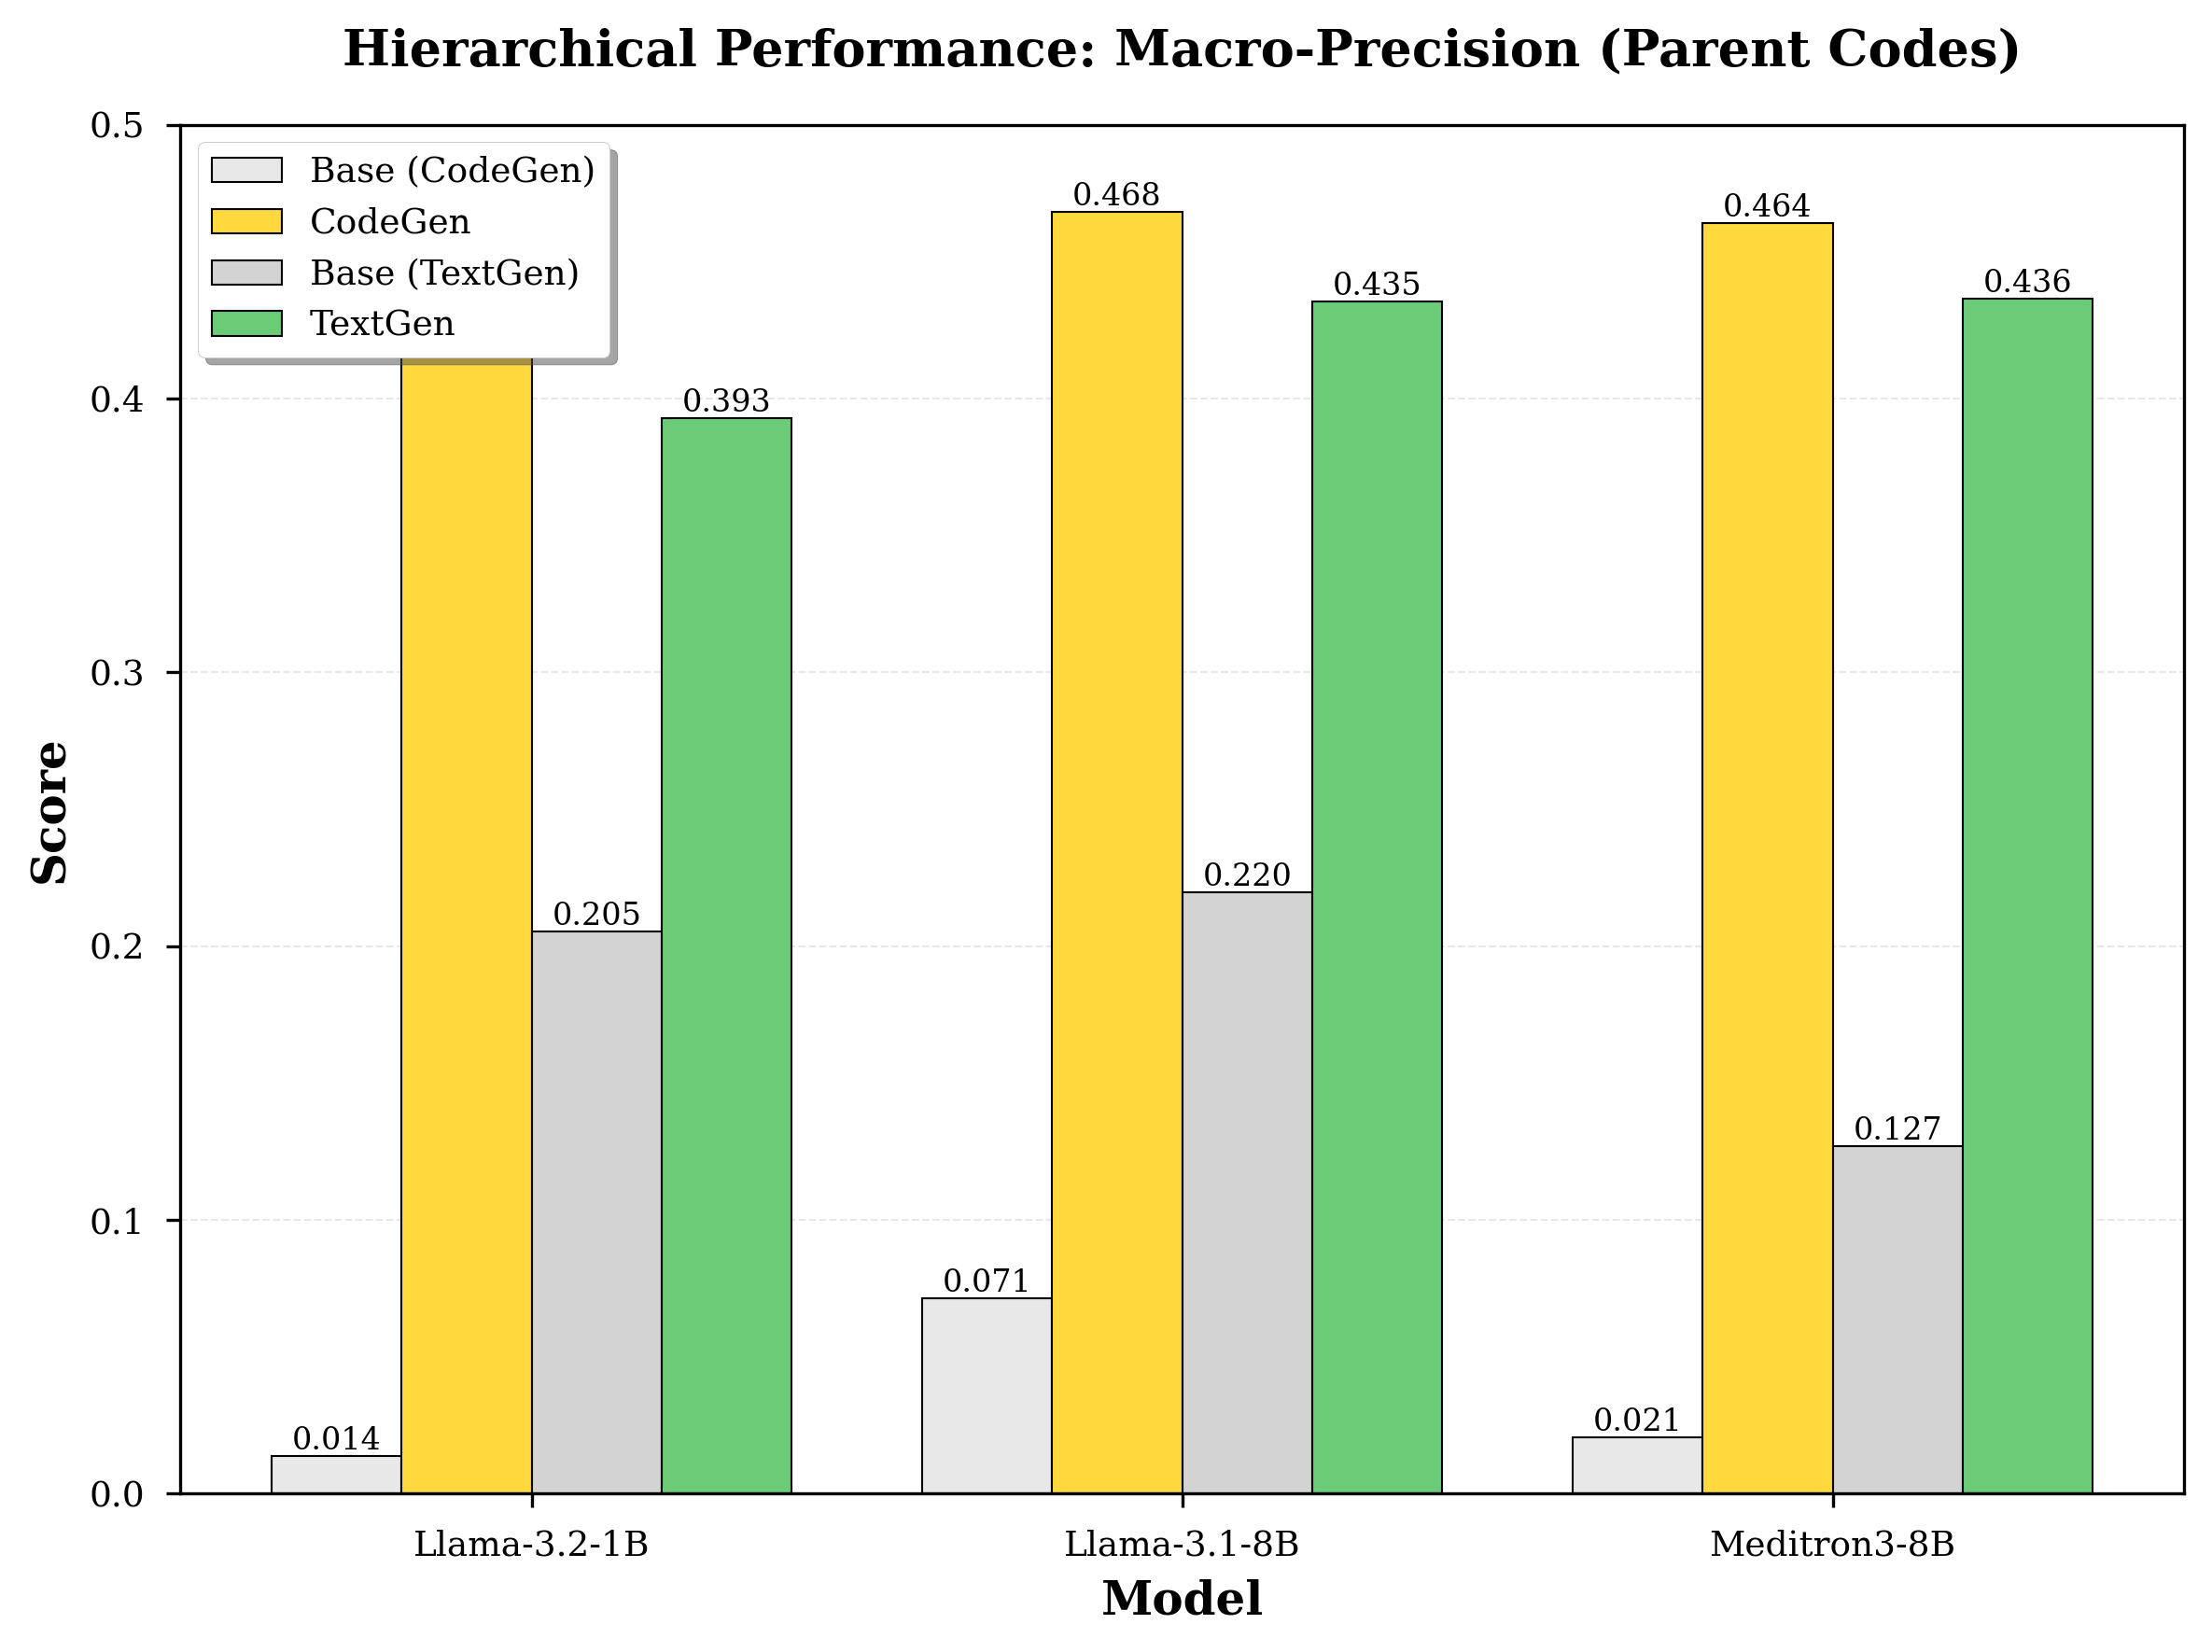
\includegraphics[width=\linewidth]{Images/Plots_thesis/parent_macro_precision.png}
%         \caption{Parent macro-Precision}
%         \label{fig:task1-parent-macroP}
%     \end{subfigure}\hfill
%     \begin{subfigure}{0.32\textwidth}
%         \centering
%         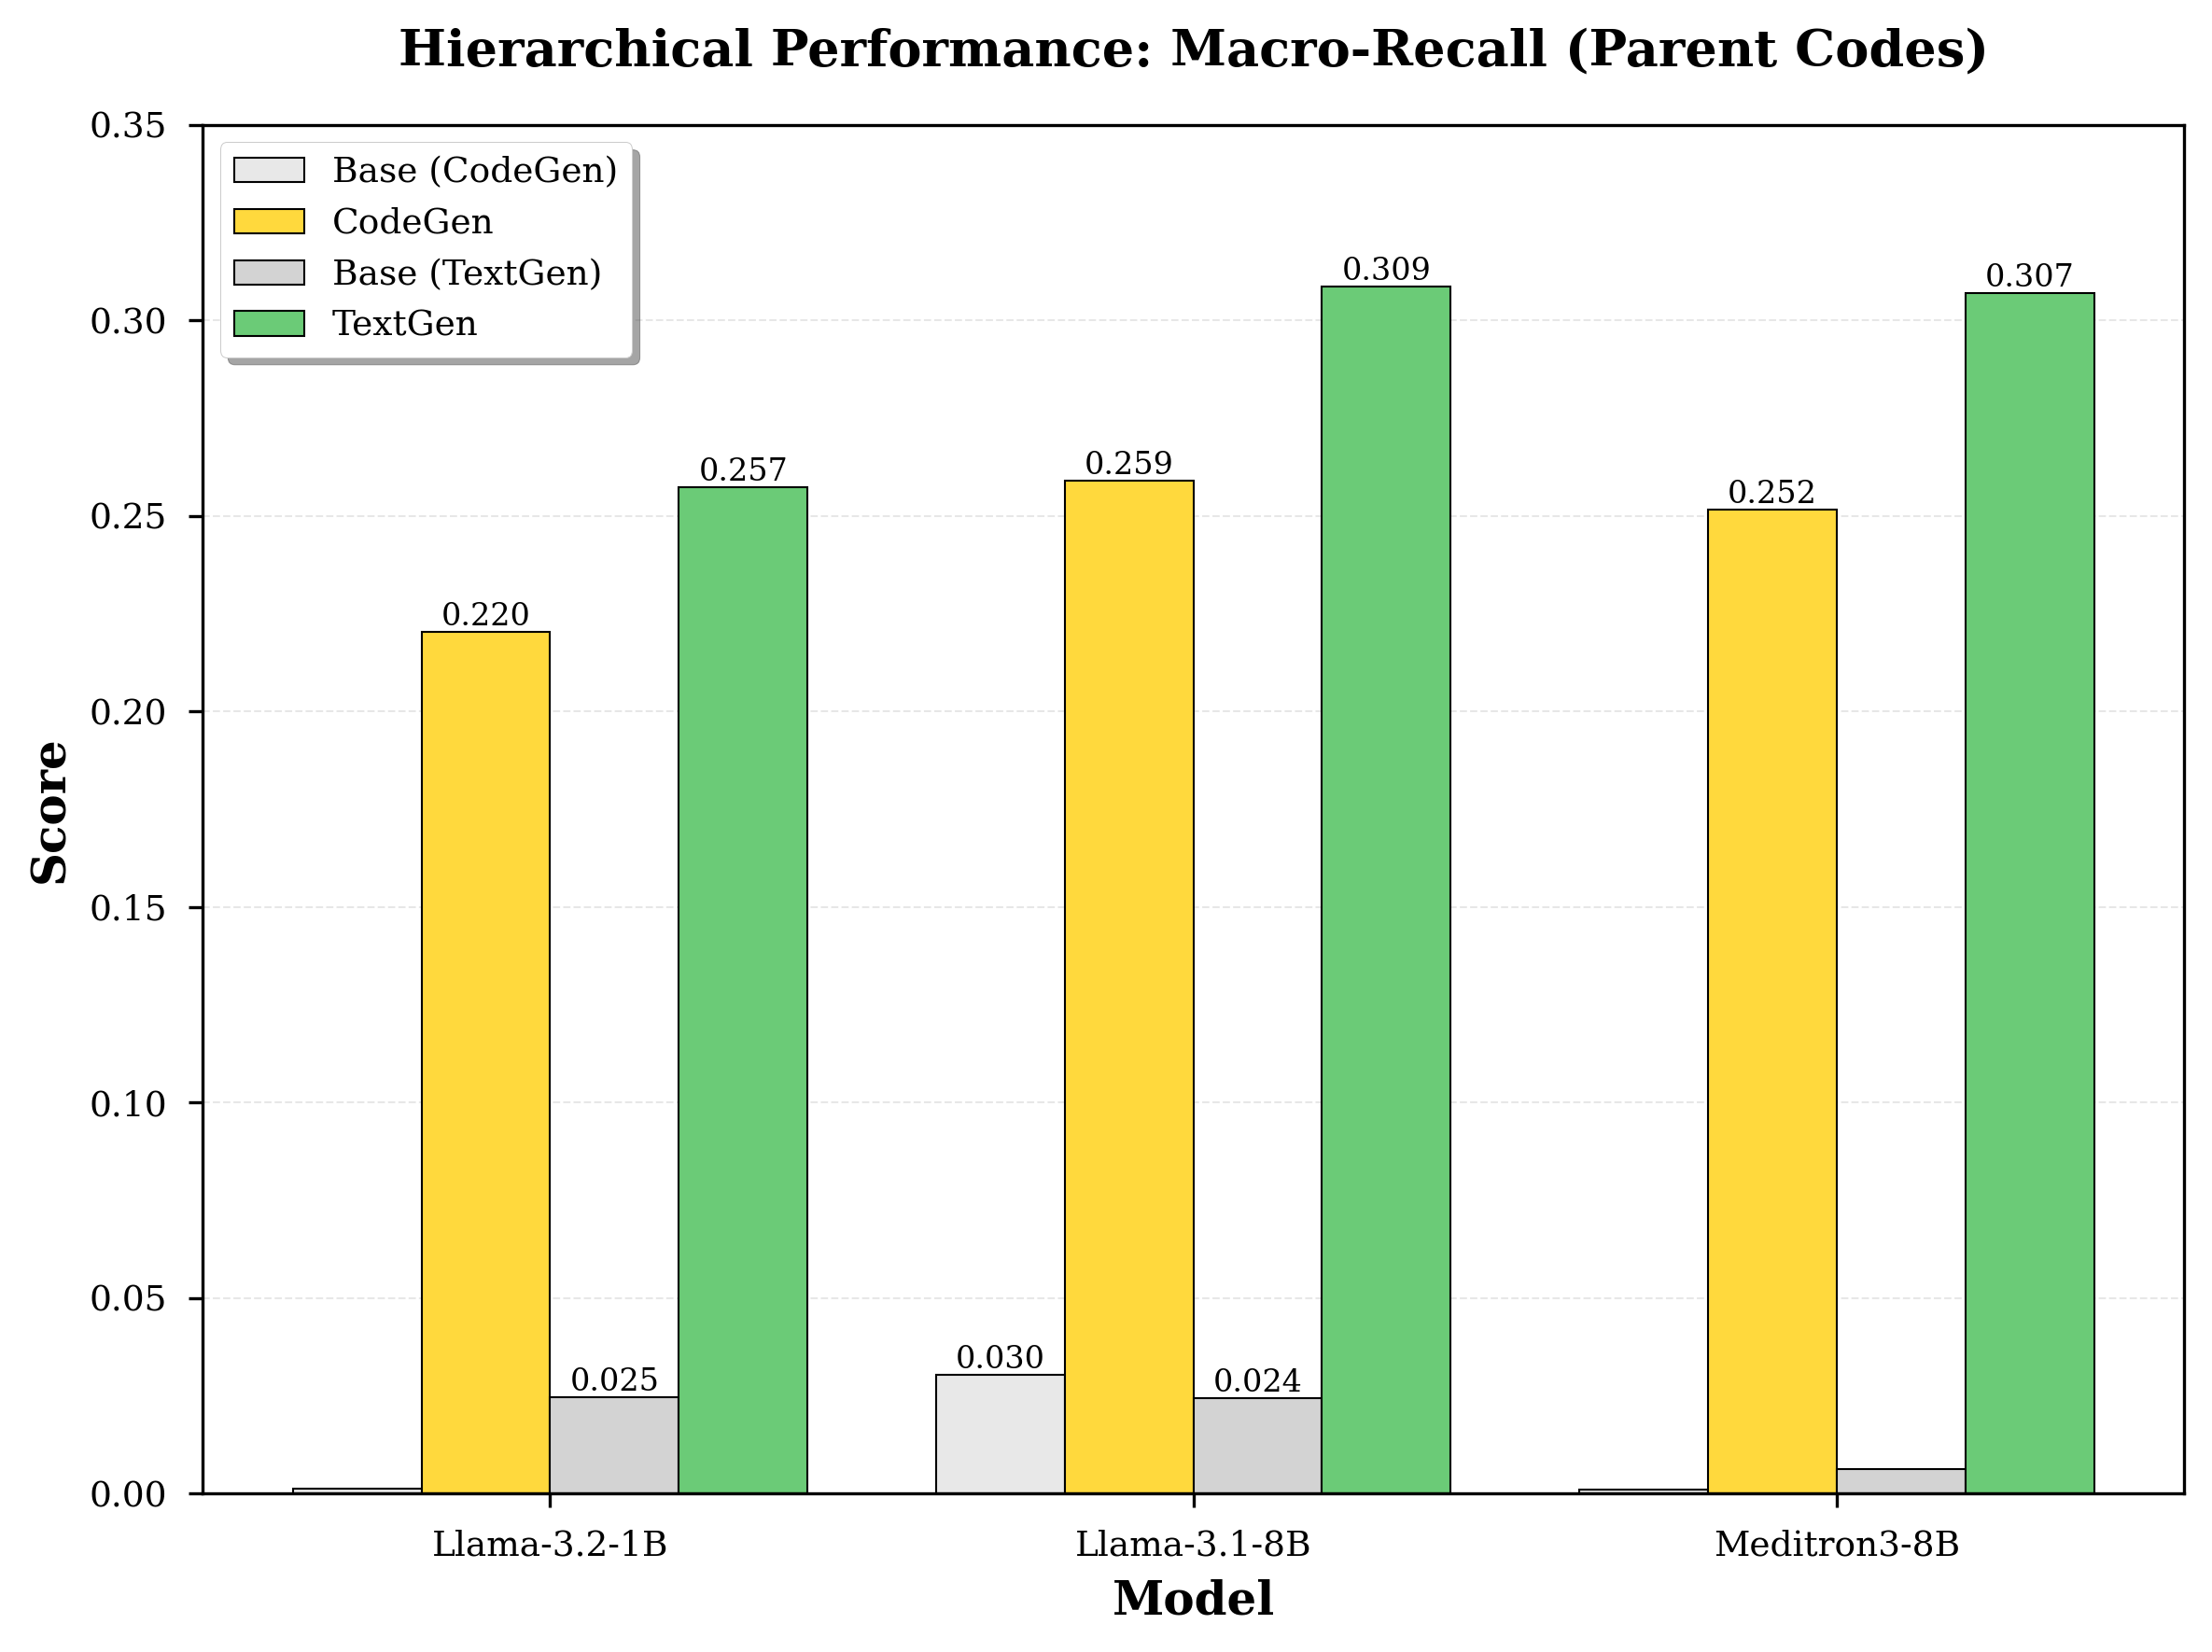
\includegraphics[width=\linewidth]{Images/Plots_thesis/parent_macro_recall.png}
%         \caption{Parent macro-Recall}
%         \label{fig:task1-parent-macroR}
%     \end{subfigure}\hfill
%     \begin{subfigure}{0.32\textwidth}
%         \centering
%         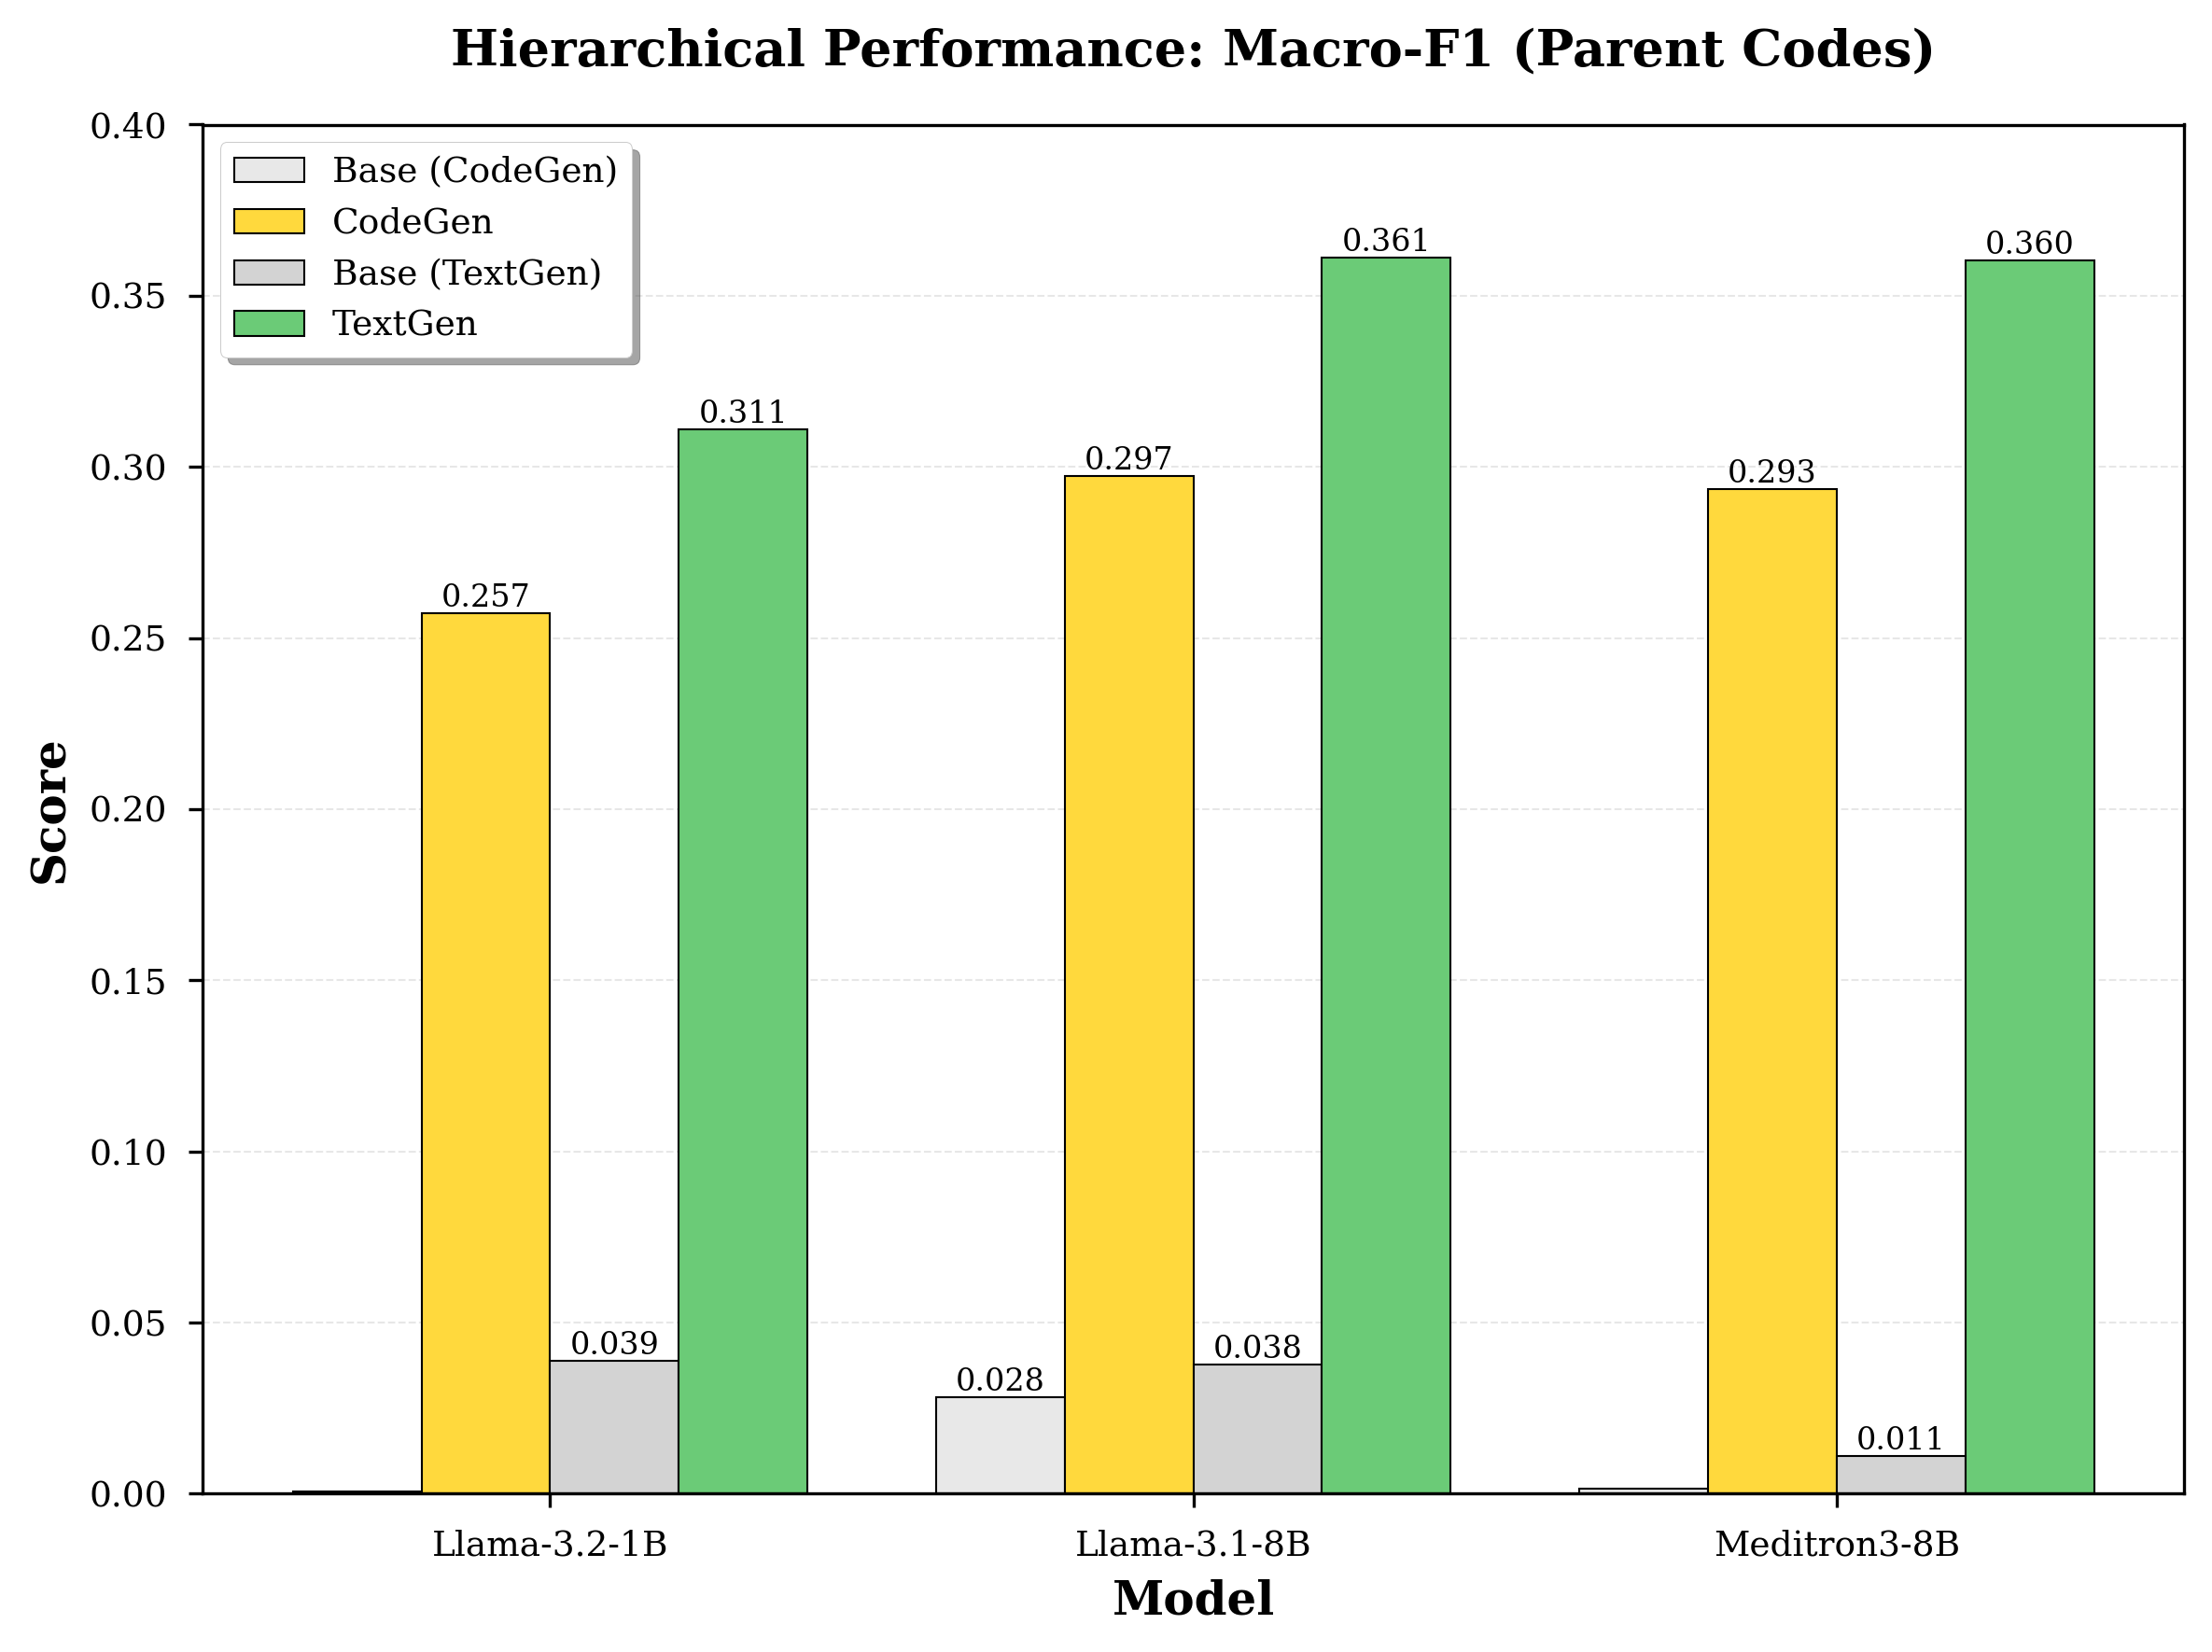
\includegraphics[width=\linewidth]{Images/Plots_thesis/parent_macro_f1.png}
%         \caption{Parent macro-F1}
%         \label{fig:task1-parent-macroF1}
%     \end{subfigure}

%     \caption{Task~1 hierarchical evaluation: parent-level micro/macro precision, recall, and F1 for \textbf{Base}, \textbf{CodeGen}, and \textbf{TextGen} across backbones. Parent evaluation reveals clinically meaningful ``near misses'' at the full-code level.}
%     \label{fig:task1-parent-metrics}
% \end{figure}

% % ============================================================
% \subsection{Head--Tail Behaviour: Performance on Frequent vs.\ Rare Codes}
% \label{subsec:results-task1-headtail}

% Overall micro-averaged metrics are dominated by frequent codes, while macro-averaged metrics are sensitive to poor tail performance. To explicitly characterise label imbalance, we evaluate models on two extremal subsets of the label space: the \textbf{Top-50} (Head-50) and \textbf{Bottom-50} (Tail-50) ICD-9 codes, defined by global code frequency across all splits (Section~\ref{subsec:head-tail-cohort}). 

% \paragraph{Top-50 codes (Head-50).}
% Table~\ref{tab:task1-top50} shows that TextGen achieves strong performance on frequent diagnoses across all backbones and substantially exceeds CodeGen. This indicates that when sufficient supervised signal exists, TextGen can use its limited output budget effectively to prioritise prevalent diagnoses.

% \begin{table}[t]
% \centering
% \caption{Task~1 performance restricted to the Top-50 most frequent ICD-9 codes (Head-50) on the test set.}
% \label{tab:task1-top50}
% \begin{tabular}{llcc}
% \toprule
% \textbf{Backbone} & \textbf{Method} & \textbf{Micro-F1} & \textbf{Macro-F1} \\
% \midrule
% \multirow{4}{*}{Llama-3.2-1B}
% & Base (CodeGen) & 0.0002 & 0.0001 \\
% & CodeGen        & 0.3292 & 0.2670 \\
% & Base (TextGen) & 0.0496 & 0.0351 \\
% & TextGen        & \textbf{0.5329} & \textbf{0.4846} \\
% \midrule
% \multirow{4}{*}{Llama-3.1-8B}
% & Base (CodeGen) & 0.0646 & 0.0315 \\
% & CodeGen        & 0.3413 & 0.2784 \\
% & Base (TextGen) & 0.0439 & 0.0300 \\
% & TextGen        & \textbf{0.5876} & \textbf{0.5347} \\
% \midrule
% \multirow{4}{*}{Meditron-8B}
% & Base (CodeGen) & 0.0101 & 0.0054 \\
% & CodeGen        & 0.3342 & 0.2723 \\
% & Base (TextGen) & 0.0030 & 0.0028 \\
% & TextGen        & \textbf{0.5845} & \textbf{0.5253} \\
% \bottomrule
% \end{tabular}
% \end{table}

% \paragraph{Bottom-50 codes (Tail-50).}
% Table~\ref{tab:task1-bottom50} reveals sharp degradation on rare diagnoses. Tail-50 values can be extremely small because each rare code has low support in the test set; even a small number of additional correct predictions can change tail micro/macro metrics substantially. Nevertheless, the consistent head--tail gap confirms that rare-code recovery is a core bottleneck under both data sparsity and a strict 12-output constraint, motivating knowledge augmentation as a targeted mechanism to improve tail coverage.

% \begin{table}[t]
% \centering
% \caption{Task~1 performance restricted to the Bottom-50 rarest ICD-9 codes (Tail-50) on the test set.}
% \label{tab:task1-bottom50}
% \begin{tabular}{llcc}
% \toprule
% \textbf{Backbone} & \textbf{Method} & \textbf{Micro-F1} & \textbf{Macro-F1} \\
% \midrule
% \multirow{4}{*}{Llama-3.2-1B}
% & Base (CodeGen) & 0.0000 & 0.0000 \\
% & CodeGen        & \textbf{0.1304} & \textbf{0.0367} \\
% & Base (TextGen) & 0.0000 & 0.0000 \\
% & TextGen        & 0.0000 & 0.0000 \\
% \midrule
% \multirow{4}{*}{Llama-3.1-8B}
% & Base (CodeGen) & 0.0129 & 0.0025 \\
% & CodeGen        & 0.1200 & 0.0600 \\
% & Base (TextGen) & 0.0488 & 0.0345 \\
% & TextGen        & \textbf{0.1200} & \textbf{0.0713} \\
% \midrule
% \multirow{4}{*}{Meditron-8B}
% & Base (CodeGen) & 0.0000 & 0.0000 \\
% & CodeGen        & 0.1304 & 0.0133 \\
% & Base (TextGen) & 0.0000 & 0.0000 \\
% & TextGen        & \textbf{0.1429} & \textbf{0.0747} \\
% \bottomrule
% \end{tabular}
% \end{table}

% \begin{figure}[t]
%     \centering
%     
\includegraphics[width=0.85\textwidth]{Images/Empty.png}
%     \caption{(Placeholder) Task~1: explicit Head-50 vs Tail-50 comparison (e.g., micro-F1 and macro-F1) across CodeGen vs TextGen and backbones. This figure should highlight the magnitude of the head--tail gap.}
%     \label{fig:task1-headtail-gap}
% \end{figure}

% % ============================================================
% \subsection{Knowledge-Augmented Prompting: KG/RAG Variants on TextGen}
% \label{subsec:results-task1-kg}

% We now evaluate whether adding KG-derived context to the prompt improves diagnosis prediction. Intuitively, KG augmentation can help under the \textbf{12-output budget} by (i) improving \emph{prioritisation} of clinically linked diagnoses and (ii) providing relational cues that are underrepresented in supervision for rare codes. We compare two KG retrieval scopes (\textbf{H1} vs.\ \textbf{H2}) and two fact-integration strategies (\textbf{Unweighted} vs.\ \textbf{Weighted}) against the \textbf{Baseline TextGen} system.

% \paragraph{Overall code-level performance.}
% Table~\ref{tab:task1-rag-overall} shows consistent improvements over Baseline TextGen across all backbones. In particular, \textbf{Weighted} variants yield the strongest gains, suggesting that controlling KG noise and promoting more relevant facts helps both precision and recall.

% \begin{table}[t]
% \centering
% \caption{Task~1 overall code-level metrics for KG-augmented (RAG) variants vs.\ Baseline TextGen (test set).}
% \label{tab:task1-rag-overall}
% \resizebox{\textwidth}{!}{
% \begin{tabular}{llcccccc}
% \toprule
% \textbf{Model} & \textbf{Method} & \textbf{Micro-F1} & \textbf{Macro-F1} & \textbf{Micro-P} & \textbf{Macro-P} & \textbf{Micro-R} & \textbf{Macro-R} \\
% \midrule
% Llama-3.2-1B & H1 Unweighted & 0.4452 & 0.2134 & 0.5190 & 0.2862 & 0.3891 & 0.1941 \\
% Llama-3.2-1B & H1 Weighted   & \textbf{0.4749} & \textbf{0.2368} & 0.5419 & 0.3068 & 0.4230 & 0.2289 \\
% Llama-3.2-1B & H2 Unweighted & 0.4407 & 0.2143 & 0.5156 & 0.2888 & 0.3842 & 0.1940 \\
% Llama-3.2-1B & H2 Weighted   & 0.4726 & 0.2333 & 0.5462 & 0.3067 & 0.4168 & 0.2234 \\
% Llama-3.2-1B & Baseline (TextGen) & 0.3764 & 0.1807 & 0.4126 & 0.2597 & 0.3466 & 0.1799 \\
% \midrule
% Llama-3.1-8B & H1 Unweighted & 0.4732 & 0.2546 & 0.5464 & 0.3349 & 0.4168 & 0.2406 \\
% Llama-3.1-8B & H1 Weighted   & \textbf{0.5029} & \textbf{0.2762} & 0.5770 & 0.3565 & 0.4459 & 0.2615 \\
% Llama-3.1-8B & H2 Unweighted & 0.4699 & 0.2558 & 0.5426 & 0.3334 & 0.4139 & 0.2426 \\
% Llama-3.1-8B & H2 Weighted   & 0.4998 & 0.2724 & 0.5739 & 0.3541 & 0.4429 & 0.2581 \\
% Llama-3.1-8B & Baseline (TextGen) & 0.4441 & 0.2370 & 0.4942 & 0.3282 & 0.4033 & 0.2284 \\
% \midrule
% Meditron3-8B & H1 Unweighted & 0.4700 & 0.2593 & 0.5436 & 0.3424 & 0.4135 & 0.2479 \\
% Meditron3-8B & H1 Weighted   & \textbf{0.5036} & \textbf{0.2793} & 0.5765 & 0.3628 & 0.4473 & 0.2662 \\
% Meditron3-8B & H2 Unweighted & 0.4736 & 0.2563 & 0.5499 & 0.3354 & 0.4153 & 0.2433 \\
% Meditron3-8B & H2 Weighted   & 0.5023 & 0.2750 & 0.5792 & 0.3519 & 0.4437 & 0.2619 \\
% Meditron3-8B & Baseline (TextGen) & 0.4440 & 0.2382 & 0.5012 & 0.3192 & 0.3986 & 0.2318 \\
% \bottomrule
% \end{tabular}}
% \end{table}

% \begin{figure}[t]
%     \centering
%     
\includegraphics[width=0.92\textwidth]{Images/Empty.png}
%     \caption{(Placeholder) KG/RAG overall metrics: grouped bars (micro/macro P/R/F1) comparing Baseline TextGen vs.\ H1/H2 Unweighted vs.\ H1/H2 Weighted per backbone.}
%     \label{fig:task1-rag-overall-plots}
% \end{figure}

% \paragraph{Hierarchical (parent-level) performance.}
% Table~\ref{tab:task1-rag-parent} shows that KG augmentation improves parent-level alignment as well. This supports the interpretation that KG context is not merely affecting code formatting, but improving clinically coherent diagnosis-family prediction. Again, \textbf{Weighted} variants are strongest across backbones.

% \begin{table}[t]
% \centering
% \caption{Task~1 parent-level hierarchical metrics for KG-augmented (RAG) variants vs.\ Baseline TextGen (test set).}
% \label{tab:task1-rag-parent}
% \resizebox{\textwidth}{!}{
% \begin{tabular}{llcccccc}
% \toprule
% \textbf{Model} & \textbf{Method} & \textbf{Micro-F1} & \textbf{Macro-F1} & \textbf{Micro-P} & \textbf{Macro-P} & \textbf{Micro-R} & \textbf{Macro-R} \\
% \midrule
% Llama-3.2-1B & H1 Unweighted & 0.5388 & 0.3174 & 0.6320 & 0.4162 & 0.4688 & 0.2874 \\
% Llama-3.2-1B & H1 Weighted   & \textbf{0.5736} & \textbf{0.3412} & 0.6571 & 0.4351 & 0.5092 & 0.3155 \\
% Llama-3.2-1B & H2 Unweighted & 0.5389 & 0.3174 & 0.6323 & 0.4163 & 0.4688 & 0.2874 \\
% Llama-3.2-1B & H2 Weighted   & 0.5708 & 0.3401 & 0.6574 & 0.4388 & 0.5012 & 0.3110 \\
% Llama-3.2-1B & Baseline (TextGen) & 0.4800 & 0.2732 & 0.5326 & 0.3845 & 0.4369 & 0.2610 \\
% \midrule
% Llama-3.1-8B & H1 Unweighted & 0.5632 & 0.3617 & 0.6463 & 0.4622 & 0.4985 & 0.3333 \\
% Llama-3.1-8B & H1 Weighted   & \textbf{0.5926} & \textbf{0.3788} & 0.6765 & 0.4757 & 0.5278 & 0.3507 \\
% Llama-3.1-8B & H2 Unweighted & 0.5598 & 0.3663 & 0.6425 & 0.4621 & 0.4955 & 0.3373 \\
% Llama-3.1-8B & H2 Weighted   & 0.5900 & 0.3789 & 0.6742 & 0.4817 & 0.5247 & 0.3505 \\
% Llama-3.1-8B & Baseline (TextGen) & 0.5388 & 0.3459 & 0.6024 & 0.4626 & 0.4873 & 0.3225 \\
% \midrule
% Meditron3-8B & H1 Unweighted & 0.5591 & 0.3720 & 0.6430 & 0.4691 & 0.4941 & 0.3480 \\
% Meditron3-8B & H1 Weighted   & \textbf{0.5931} & \textbf{0.3902} & 0.6757 & 0.4907 & 0.5288 & 0.3655 \\
% Meditron3-8B & H2 Unweighted & 0.5631 & 0.3622 & 0.6478 & 0.4475 & 0.4975 & 0.3380 \\
% Meditron3-8B & H2 Weighted   & 0.5910 & 0.3835 & 0.6764 & 0.4742 & 0.5249 & 0.3597 \\
% Meditron3-8B & Baseline (TextGen) & 0.5364 & 0.3418 & 0.6064 & 0.4407 & 0.4809 & 0.3224 \\
% \bottomrule
% \end{tabular}}
% \end{table}

% \begin{figure}[t]
%     \centering
%     
\includegraphics[width=0.92\textwidth]{Images/Empty.png}
%     \caption{(Placeholder) KG/RAG parent-level metrics: grouped bars (micro/macro P/R/F1) comparing Baseline vs.\ KG variants per backbone.}
%     \label{fig:task1-rag-parent-plots}
% \end{figure}

% \paragraph{Head-50 (frequent) vs.\ Tail-50 (rare) effects under KG augmentation.}
% Tables~\ref{tab:task1-rag-top50} and \ref{tab:task1-rag-tail50} decompose KG gains by frequency strata. KG augmentation improves Head-50 metrics (consistent but moderate), while improvements on Tail-50 are particularly important because they indicate progress on rare codes beyond what can be explained by head dominance alone.

% \begin{table}[t]
% \centering
% \caption{Task~1 Top-50 codes (Head-50) metrics for KG-augmented variants vs.\ Baseline TextGen (test set).}
% \label{tab:task1-rag-top50}
% \resizebox{\textwidth}{!}{
% \begin{tabular}{llcccccc}
% \toprule
% \textbf{Model} & \textbf{Method} & \textbf{Micro-F1} & \textbf{Macro-F1} & \textbf{Micro-P} & \textbf{Macro-P} & \textbf{Micro-R} & \textbf{Macro-R} \\
% \midrule
% Llama-3.2-1B & H1 Unweighted & 0.6009 & 0.5473 & 0.6308 & 0.6134 & 0.5729 & 0.5110 \\
% Llama-3.2-1B & H1 Weighted   & \textbf{0.6375} & \textbf{0.5839} & 0.6590 & 0.6391 & 0.6173 & 0.5563 \\
% Llama-3.2-1B & H2 Unweighted & 0.6005 & 0.5474 & 0.6337 & 0.6159 & 0.5700 & 0.5117 \\
% Llama-3.2-1B & H2 Weighted   & 0.6334 & 0.5799 & 0.6637 & 0.6451 & 0.6055 & 0.5451 \\
% Llama-3.2-1B & Baseline (TextGen) & 0.5329 & 0.4846 & 0.5645 & 0.5874 & 0.5047 & 0.4584 \\
% \midrule
% Llama-3.1-8B & H1 Unweighted & 0.6259 & 0.5683 & 0.6513 & 0.6323 & 0.6017 & 0.5387 \\
% Llama-3.1-8B & H1 Weighted   & \textbf{0.6535} & \textbf{0.5952} & 0.6780 & 0.6608 & 0.6308 & 0.5669 \\
% Llama-3.1-8B & H2 Unweighted & 0.6209 & 0.5635 & 0.6468 & 0.6282 & 0.5974 & 0.5340 \\
% Llama-3.1-8B & H2 Weighted   & 0.6500 & 0.5927 & 0.6720 & 0.6562 & 0.6294 & 0.5652 \\
% Llama-3.1-8B & Baseline (TextGen) & 0.5876 & 0.5347 & 0.5997 & 0.6099 & 0.5759 & 0.5161 \\
% \midrule
% Meditron3-8B & H1 Unweighted & 0.6162 & 0.5596 & 0.6430 & 0.6231 & 0.5914 & 0.5288 \\
% Meditron3-8B & H1 Weighted   & \textbf{0.6529} & \textbf{0.5954} & 0.6791 & 0.6611 & 0.6288 & 0.5648 \\
% Meditron3-8B & H2 Unweighted & 0.6238 & 0.5673 & 0.6523 & 0.6339 & 0.5976 & 0.5352 \\
% Meditron3-8B & H2 Weighted   & \textbf{0.6529} & 0.5946 & 0.6826 & 0.6624 & 0.6257 & 0.5636 \\
% Meditron3-8B & Baseline (TextGen) & 0.5845 & 0.5253 & 0.6103 & 0.6149 & 0.5608 & 0.4983 \\
% \bottomrule
% \end{tabular}}
% \end{table}

% \begin{table}[t]
% \centering
% \caption{Task~1 Bottom-50 codes (Tail-50) metrics for KG-augmented variants vs.\ Baseline TextGen (test set).}
% \label{tab:task1-rag-tail50}
% \resizebox{\textwidth}{!}{
% \begin{tabular}{llcccccc}
% \toprule
% \textbf{Model} & \textbf{Method} & \textbf{Micro-F1} & \textbf{Macro-F1} & \textbf{Micro-P} & \textbf{Macro-P} & \textbf{Micro-R} & \textbf{Macro-R} \\
% \midrule
% Llama-3.2-1B & H1 Unweighted & 0.1304 & 0.0427 & 0.3333 & 0.0345 & 0.0811 & 0.0575 \\
% Llama-3.2-1B & H1 Weighted   & 0.1509 & 0.0740 & 0.4100 & 0.0880 & 0.0950 & 0.0695 \\
% Llama-3.2-1B & H2 Unweighted & 0.1702 & 0.0747 & 0.4000 & 0.0977 & 0.1081 & 0.0747 \\
% Llama-3.2-1B & H2 Weighted   & \textbf{0.1841} & \textbf{0.0865} & 0.4200 & 0.1050 & 0.1150 & 0.0805 \\
% Llama-3.2-1B & Baseline (TextGen) & 0.0000 & 0.0000 & 0.0000 & 0.0000 & 0.0000 & 0.0000 \\
% \midrule
% Llama-3.1-8B & H1 Unweighted & 0.1364 & 0.0747 & 0.4286 & 0.1034 & 0.0811 & 0.0632 \\
% Llama-3.1-8B & H1 Weighted   & 0.1689 & 0.1140 & 0.3600 & 0.1450 & 0.1100 & 0.1010 \\
% Llama-3.1-8B & H2 Unweighted & 0.1304 & 0.0747 & 0.3333 & 0.1034 & 0.0811 & 0.0632 \\
% Llama-3.1-8B & H2 Weighted   & \textbf{0.1820} & \textbf{0.1215} & 0.3500 & 0.1520 & 0.1220 & 0.1085 \\
% Llama-3.1-8B & Baseline (TextGen) & 0.1200 & 0.0713 & 0.2308 & 0.0862 & 0.0811 & 0.0632 \\
% \midrule
% Meditron3-8B & H1 Unweighted & 0.1739 & 0.0920 & 0.4444 & 0.1379 & 0.1081 & 0.0747 \\
% Meditron3-8B & H1 Weighted   & \textbf{0.1915} & \textbf{0.1220} & 0.4100 & 0.1600 & 0.1250 & 0.1080 \\
% Meditron3-8B & H2 Unweighted & 0.1778 & 0.1092 & 0.5000 & 0.1379 & 0.1081 & 0.0977 \\
% Meditron3-8B & H2 Weighted   & 0.1890 & 0.1185 & 0.4600 & 0.1550 & 0.1200 & 0.1060 \\
% Meditron3-8B & Baseline (TextGen) & 0.1429 & 0.0747 & 0.6000 & 0.1034 & 0.0811 & 0.0632 \\
% \bottomrule
% \end{tabular}}
% \end{table}

% \begin{figure}[t]
%     \centering
%     
\includegraphics[width=0.92\textwidth]{Images/Empty.png}
%     \caption{(Placeholder) KG/RAG head--tail plots: Head-50 vs Tail-50 micro-F1 (and/or macro-F1) for Baseline vs.\ KG variants.}
%     \label{fig:task1-rag-headtail-plots}
% \end{figure}

% \paragraph{Interpretation of tail improvements and clinical impact.}
% The Tail-50 results are the most diagnostic for whether KG augmentation addresses the long tail. Two patterns stand out:
% \begin{itemize}
%     \item \textbf{Tail gains are largest (in relative terms) for the stronger backbones.} For \texttt{Llama-3.1-8B} and \texttt{Meditron-8B}, Tail-50 micro-F1 improves substantially over the Baseline TextGen system (Table~\ref{tab:task1-rag-tail50}), indicating that KG cues can help recover rare diagnoses that are otherwise missed under sparse supervision.
%     \item \textbf{Weighting matters for rare codes.} Weighted variants consistently outperform unweighted ones on Tail-50 macro-F1 across backbones, suggesting that relevance-weighted fact selection reduces noise and helps allocate the 12-output budget toward more diagnostically informative candidates.
% \end{itemize}
% Even though absolute Tail-50 scores remain modest (rare-code recovery is still difficult), the consistent directional improvement supports the thesis hypothesis that structured knowledge can partially compensate for limited tail supervision.

% % ============================================================
% \subsection{Interaction with Multimorbidity and the 12-Diagnosis Output Budget}
% \label{subsec:results-task1-budget}

% Because models are instructed to output at most 12 diagnoses per admission, admissions with more than 12 gold codes impose an intrinsic upper bound on achievable recall:
% \[
% R^{\max(i)} = \min\left(1, \frac{12}{L^{(i)}}\right),
% \]
% where $L^{(i)}$ is the number of gold diagnoses for admission $i$.
% This constraint makes evaluation more realistic (clinical tools cannot output arbitrarily many diagnoses) but implies that improvements in recall must arise from \emph{prioritisation}. KG augmentation is especially relevant here: relational cues can guide the model toward a better ordering/selection of diagnoses under a strict output budget.

% \begin{figure}[t]
%     \centering
%     
\includegraphics[width=0.85\textwidth]{Images/Empty.png}
%     \caption{(Placeholder) Task~1: performance stratified by admission complexity (bins based on number of diagnoses per admission). Report at least micro-recall and micro-F1 per bin for Baseline TextGen vs.\ best KG variant.}
%     \label{fig:task1-complexity-stratified}
% \end{figure}

% % ============================================================
% \subsection{Robustness Notes for Rare-Code Evaluation}
% \label{subsec:results-task1-robustness}

% Tail-code evaluation is inherently high-variance because each rare code has low support in the test set. As a result:
% \begin{itemize}
%     \item \textbf{Tail-50 macro-F1 can fluctuate strongly} with a small number of additional correct predictions.
%     \item \textbf{Tail improvements should be interpreted with uncertainty}, especially when comparing close variants (e.g., H1 vs H2).
% \end{itemize}

% To address this transparently, we recommend reporting uncertainty using \textbf{bootstrap confidence intervals over admissions} (resample test admissions with replacement; recompute metrics). This produces an uncertainty band for statements such as ``KG augmentation improves Tail-50 micro-F1'' and is especially important for tail-focused conclusions.

% \begin{table}[t]
% \centering
% \caption{(Placeholder) Bootstrap confidence intervals (95\%) for key Task~1 metrics. Recommended: Baseline TextGen vs.\ best KG-Weighted variant on the best-performing backbone.}
% \label{tab:task1-bootstrap-ci}
% \begin{tabular}{lcc}
% \toprule
% \textbf{Metric} & \textbf{Baseline TextGen (CI)} & \textbf{Best KG Weighted (CI)} \\
% \midrule
% Overall micro-F1 & -- & -- \\
% Overall macro-F1 & -- & -- \\
% Tail-50 micro-F1 & -- & -- \\
% Tail-50 macro-F1 & -- & -- \\
% \bottomrule
% \end{tabular}
% \end{table}

% % ============================================================
% \subsection{Summary, Improvements, and Transition}
% \label{subsec:results-task1-summary}

% Task~1 results form a coherent progression:
% \begin{itemize}
%     \item \textbf{Fine-tuning is essential:} Base prompting performs poorly, especially for direct ICD generation.
%     \item \textbf{TextGen is the strongest baseline pipeline:} it consistently outperforms CodeGen at full-code and parent-code evaluation, particularly improving macro-level behaviour.
%     \item \textbf{Performance is frequency-dependent:} results are strong on Head-50 but degrade sharply on Tail-50, confirming a pronounced head--tail gap.
%     \item \textbf{KG augmentation improves both overall and tail behaviour:} KG/RAG variants yield consistent gains over Baseline TextGen across backbones, and notably improve Tail-50 metrics, supporting the hypothesis that structured relations can help recover underrepresented diagnoses under a strict 12-output budget.
% \end{itemize}

% To make improvements explicit, Table~\ref{tab:task1-delta-summary} summarises absolute ($\Delta$) and relative (\%) gains for the best-performing KG variant per backbone.\footnote{For Llama-3.2-1B Tail-50, baseline is exactly zero; percent improvement is undefined and only absolute gains are reported.}

% \begin{table}[t]
% \centering
% \caption{Summary of improvements from Baseline TextGen to the best KG-augmented variant (per backbone). Relative gains shown as percent where baseline is non-zero.}
% \label{tab:task1-delta-summary}
% \resizebox{\textwidth}{!}{
% \begin{tabular}{lcccccc}
% \toprule
% \textbf{Backbone} &
% \textbf{Overall micro-F1} & $\Delta$ (\%) &
% \textbf{Overall macro-F1} & $\Delta$ (\%) &
% \textbf{Tail-50 micro-F1} & $\Delta$ (\%) \\
% \midrule
% Llama-3.2-1B &
% 0.3764 $\rightarrow$ 0.4749 & +0.0985 (+26.17\%) &
% 0.1807 $\rightarrow$ 0.2368 & +0.0561 (+31.05\%) &
% 0.0000 $\rightarrow$ 0.1841 & +0.1841 (--) \\
% \midrule
% Llama-3.1-8B &
% 0.4441 $\rightarrow$ 0.5029 & +0.0588 (+13.24\%) &
% 0.2370 $\rightarrow$ 0.2762 & +0.0392 (+16.54\%) &
% 0.1200 $\rightarrow$ 0.1820 & +0.0620 (+51.67\%) \\
% \midrule
% Meditron3-8B &
% 0.4440 $\rightarrow$ 0.5036 & +0.0596 (+13.42\%) &
% 0.2382 $\rightarrow$ 0.2793 & +0.0411 (+17.25\%) &
% 0.1429 $\rightarrow$ 0.1915 & +0.0486 (+34.01\%) \\
% \bottomrule
% \end{tabular}}
% \end{table}

% \noindent\textbf{Conclusive statement.}
% Across all backbones, KG-augmented prompting yields a consistent and practically meaningful improvement in Task~1 diagnosis prediction. Gains are observed not only in overall micro-F1 (head-dominated performance) but also in Tail-50 metrics, indicating that KG context contributes to better coverage of rare diagnoses rather than merely amplifying frequent-code predictions. This strengthens the central premise of the thesis: \emph{structured clinical knowledge can guide LLM-based diagnosis prediction under real-world constraints (multimorbidity and limited output budget).} In the next section, we analyse these KG gains more deeply and connect them to the specific KG prompt designs and weighting strategies used.



%% ============================================================





% \section{Task~1: Current-Visit Diagnosis Prediction}
% \label{sec:results-task1}

% This section reports results for Task~1 (current-visit diagnosis prediction) under the evaluation protocol in Section~\ref{sec:evaluation}. We evaluate three modelling stages (\textbf{Base}, \textbf{CodeGen}, \textbf{TextGen}) across three backbones (\texttt{Llama-3.2-1B-Instruct}, \texttt{Llama-3.1-8B-Instruct}, \texttt{Meditron-8B}). 
% For \textbf{Base} runs, LoRA adapters are disabled (no task-specific updates). For \textbf{CodeGen} and \textbf{TextGen}, the backbones are fine-tuned with LoRA using the prompts defined in Section~\ref{sec:model-architectures}. 

% We then study whether structured knowledge improves TextGen via two steps:
% (i) an \textbf{inference-only KG ablation} where KG paths are injected at test time without changing training, and
% (ii) \textbf{KG-augmented fine-tuning (RAG-style)} where the model is trained to use KG paths (and also receives them at inference).
% This ordering is intentional: it isolates whether KG helps only when the model is explicitly trained to leverage it.

% As described in Section~\ref{subsec:complexity-cohort}, all models are instructed to generate a fixed budget of \textbf{at most 12 diagnoses per admission}. This interacts non-trivially with recall in highly multimorbid admissions: improvements in recall often require \emph{better prioritisation} under a limited output budget rather than simply generating more outputs.

% % ============================================================
% \subsection{Baseline Performance: From Raw Backbones to Fine-Tuned Pipelines}
% \label{subsec:results-task1-baselines}

% Before analysing knowledge augmentation, we quantify how well the raw instruction-tuned backbones perform on Task~1 without task-specific fine-tuning. In these \emph{Base} runs, models are used ``as is'' with the same Task~1 prompts (Section~\ref{sec:model-architectures}), but LoRA adapters are disabled. This establishes a lower bound on performance and clarifies how much of the task is solved by generic instruction-following alone.

% We evaluate four configurations per backbone:
% \begin{enumerate}
%     \item \textbf{Base (CodeGen):} raw backbone prompted to output ICD-9 codes directly (no fine-tuning).
%     \item \textbf{CodeGen:} fine-tuned pipeline generating ICD-9 codes directly from multimodal prompts (Section~\ref{subsec:codegen-arch}).
%     \item \textbf{Base (TextGen):} raw backbone prompted to output diagnosis terms (no fine-tuning), followed by SapBERT+FAISS mapping.
%     \item \textbf{TextGen:} fine-tuned pipeline generating diagnosis terms followed by SapBERT+FAISS mapping (Section~\ref{subsec:textgen-arch}).
% \end{enumerate}

% Table~\ref{tab:task1-all-methods-flat} reports micro-F1 and macro-F1 at the full ICD-9 code level (test set). Precision/recall and sample-averaged metrics are visualised in Figure~\ref{fig:task1-flat-metrics} (kept from the earlier draft).

% \begin{table}[t]
%     \centering
%     \caption{Task~1 (current-visit diagnosis prediction): comparison of raw backbones (\textbf{Base}), fine-tuned \textbf{CodeGen}, and fine-tuned \textbf{TextGen} across all backbones. Metrics are computed at the full ICD-9 code level on the held-out test set.}
%     \label{tab:task1-all-methods-flat}
%     \begin{tabular}{llcc}
%         \toprule
%         \textbf{Backbone} & \textbf{Method} &
%         \textbf{Micro-F1} & \textbf{Macro-F1} \\
%         \midrule
%         \multirow{4}{*}{Llama-3.2-1B} 
%             & Base (no FT) - Direct codes  & 0.0003 & 0.0000 \\
%             & CodeGen        & 0.2344 & 0.0151 \\
%             & Base (no FT) - Free Text  & 0.0393 & 0.0250 \\
%             & TextGen        & \textbf{0.4313} & \textbf{0.2065} \\
%         \midrule
%         \multirow{4}{*}{Llama-3.1-8B} 
%             & Base (no FT) - Direct codes  & 0.0269 & 0.0007 \\
%             & CodeGen        & 0.2487 & 0.0188 \\
%             & Base (no FT) - Free Text  & 0.0358 & 0.0244 \\
%             & TextGen        & \textbf{0.4585} & \textbf{0.2457} \\
%         \midrule
%         \multirow{4}{*}{Meditron-8B} 
%             & Base (no FT) - Direct codes  & 0.0040 & 0.0000 \\
%             & CodeGen        & 0.2475 & 0.0186 \\
%             & Base (no FT) - Free Text  & 0.0068 & 0.0071 \\
%             & TextGen        & \textbf{0.4585} & \textbf{0.2457} \\
%         \bottomrule
%     \end{tabular}
% \end{table}

% Three consistent trends emerge:
% \begin{itemize}
%     \item \textbf{Raw backbones are insufficient.} Without fine-tuning, direct-code generation is near-zero across all backbones. Base TextGen is marginally better than Base CodeGen, suggesting models can sometimes produce plausible diagnosis language, but still cannot reliably recover a large multi-label ICD space.
%     \item \textbf{Fine-tuning yields large, systematic gains.} Both CodeGen and TextGen improve substantially over their Base counterparts, confirming that task-specific supervision is essential for long clinical notes and highly imbalanced label spaces.
%     \item \textbf{TextGen consistently outperforms CodeGen.} For every backbone, TextGen achieves higher micro-F1 and macro-F1 than CodeGen. The macro-F1 gap indicates better distribution of performance beyond the head labels, consistent with the design motivation of decoupling natural-language diagnosis generation from strict code formatting.
% \end{itemize}

% % --- KEEP THESE IMAGES EXACTLY (as requested) ---
% \begin{figure}[t]
%     \centering
%     % Top row: micro-averaged metrics
%     \begin{subfigure}{0.32\textwidth}
%         \centering
%         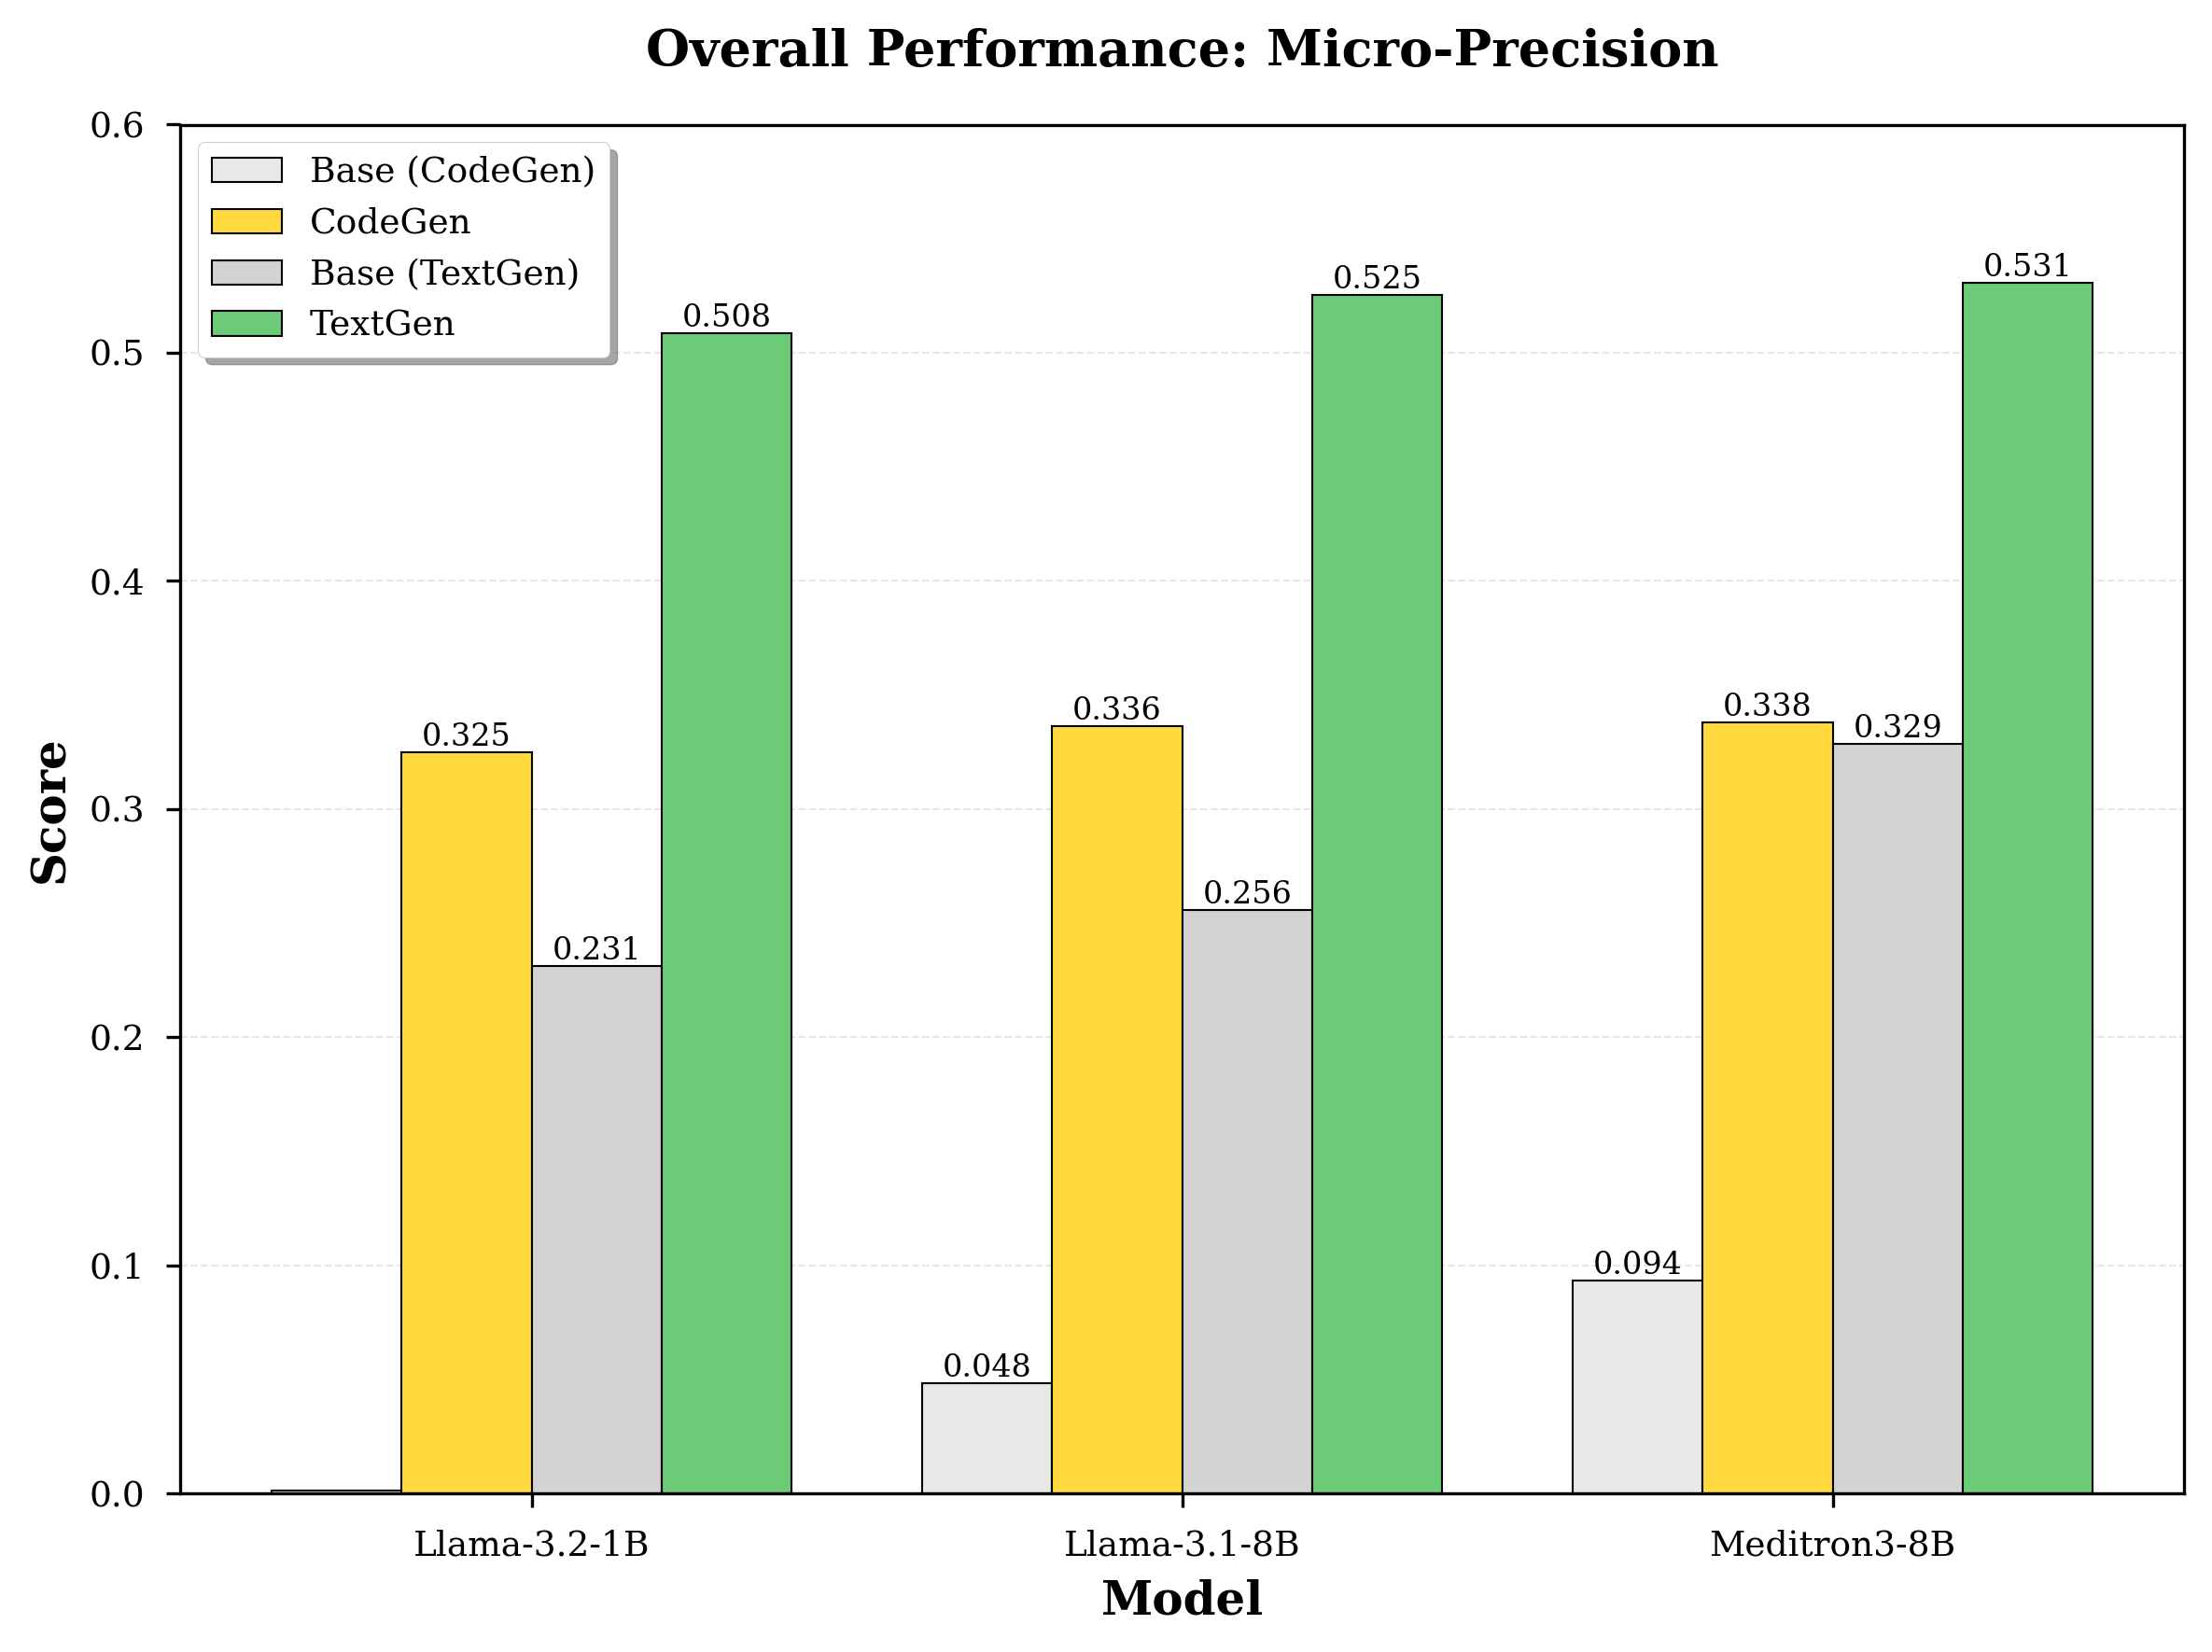
\includegraphics[width=\linewidth]{Images/Plots_thesis/overall_micro_precision.png}
%         \caption{Micro-Precision}
%         \label{fig:task1-flat-microP}
%     \end{subfigure}\hfill
%     \begin{subfigure}{0.32\textwidth}
%         \centering
%         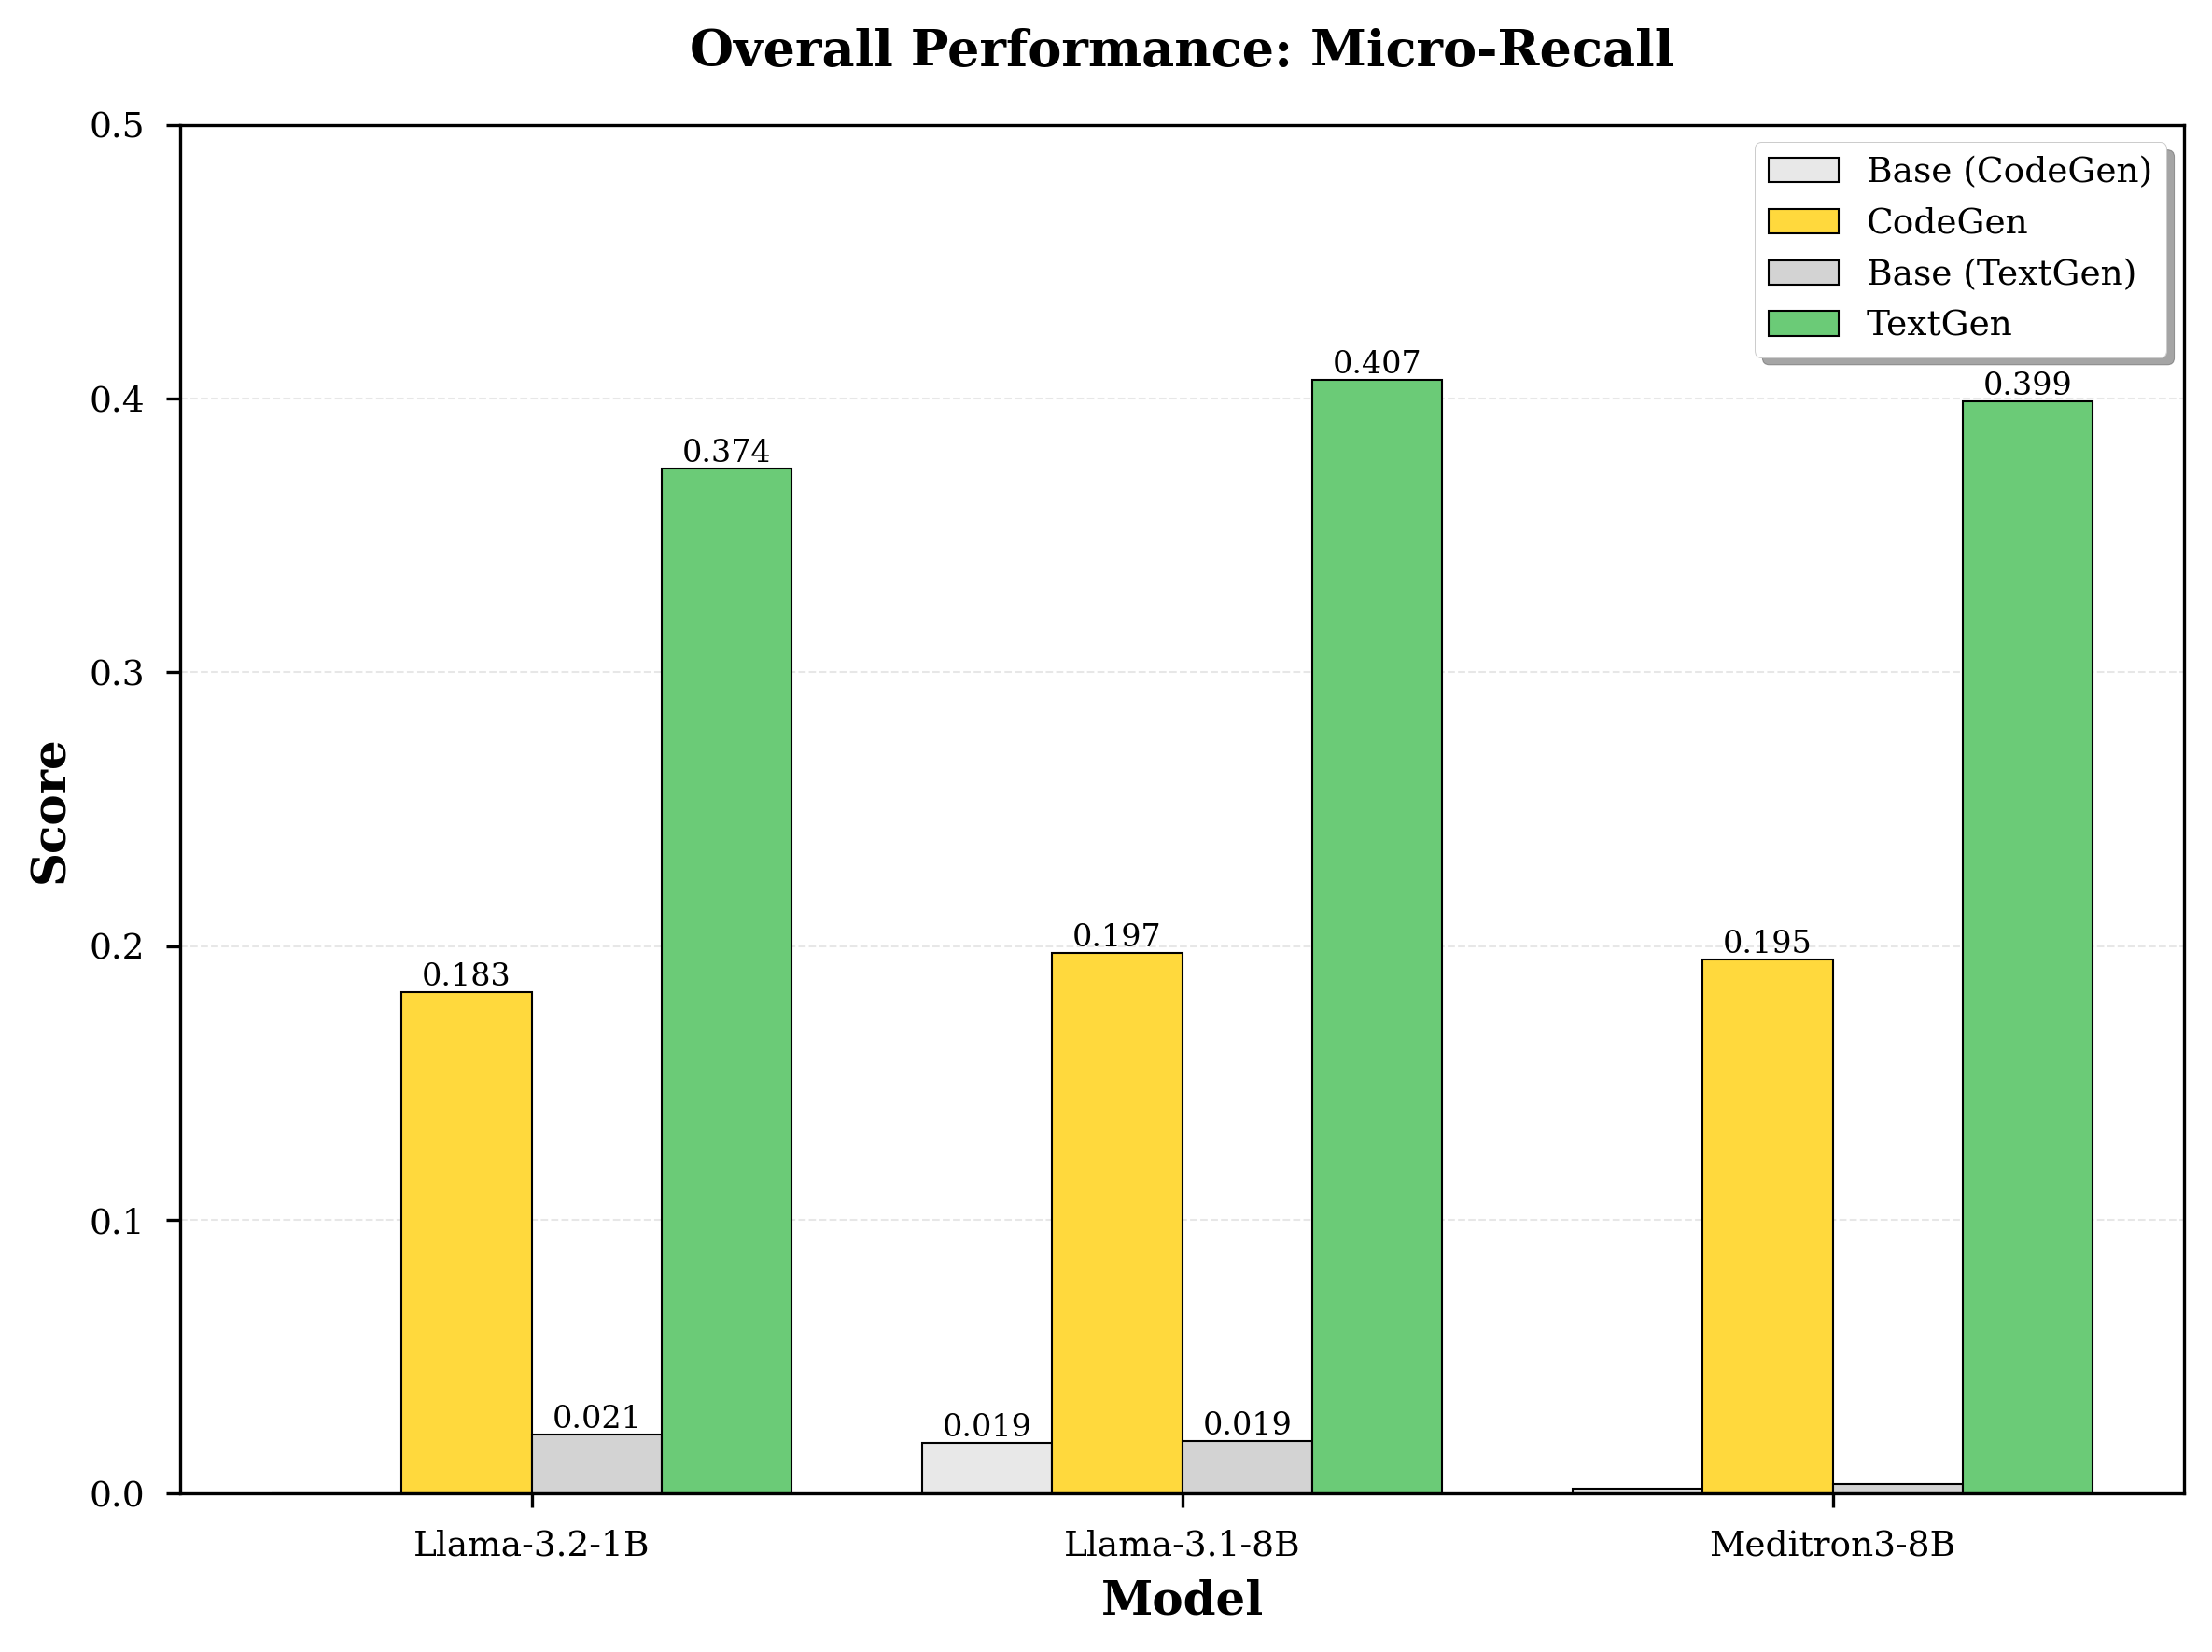
\includegraphics[width=\linewidth]{Images/Plots_thesis/overall_micro_recall.png}
%         \caption{Micro-Recall}
%         \label{fig:task1-flat-microR}
%     \end{subfigure}\hfill
%     \begin{subfigure}{0.32\textwidth}
%         \centering
%         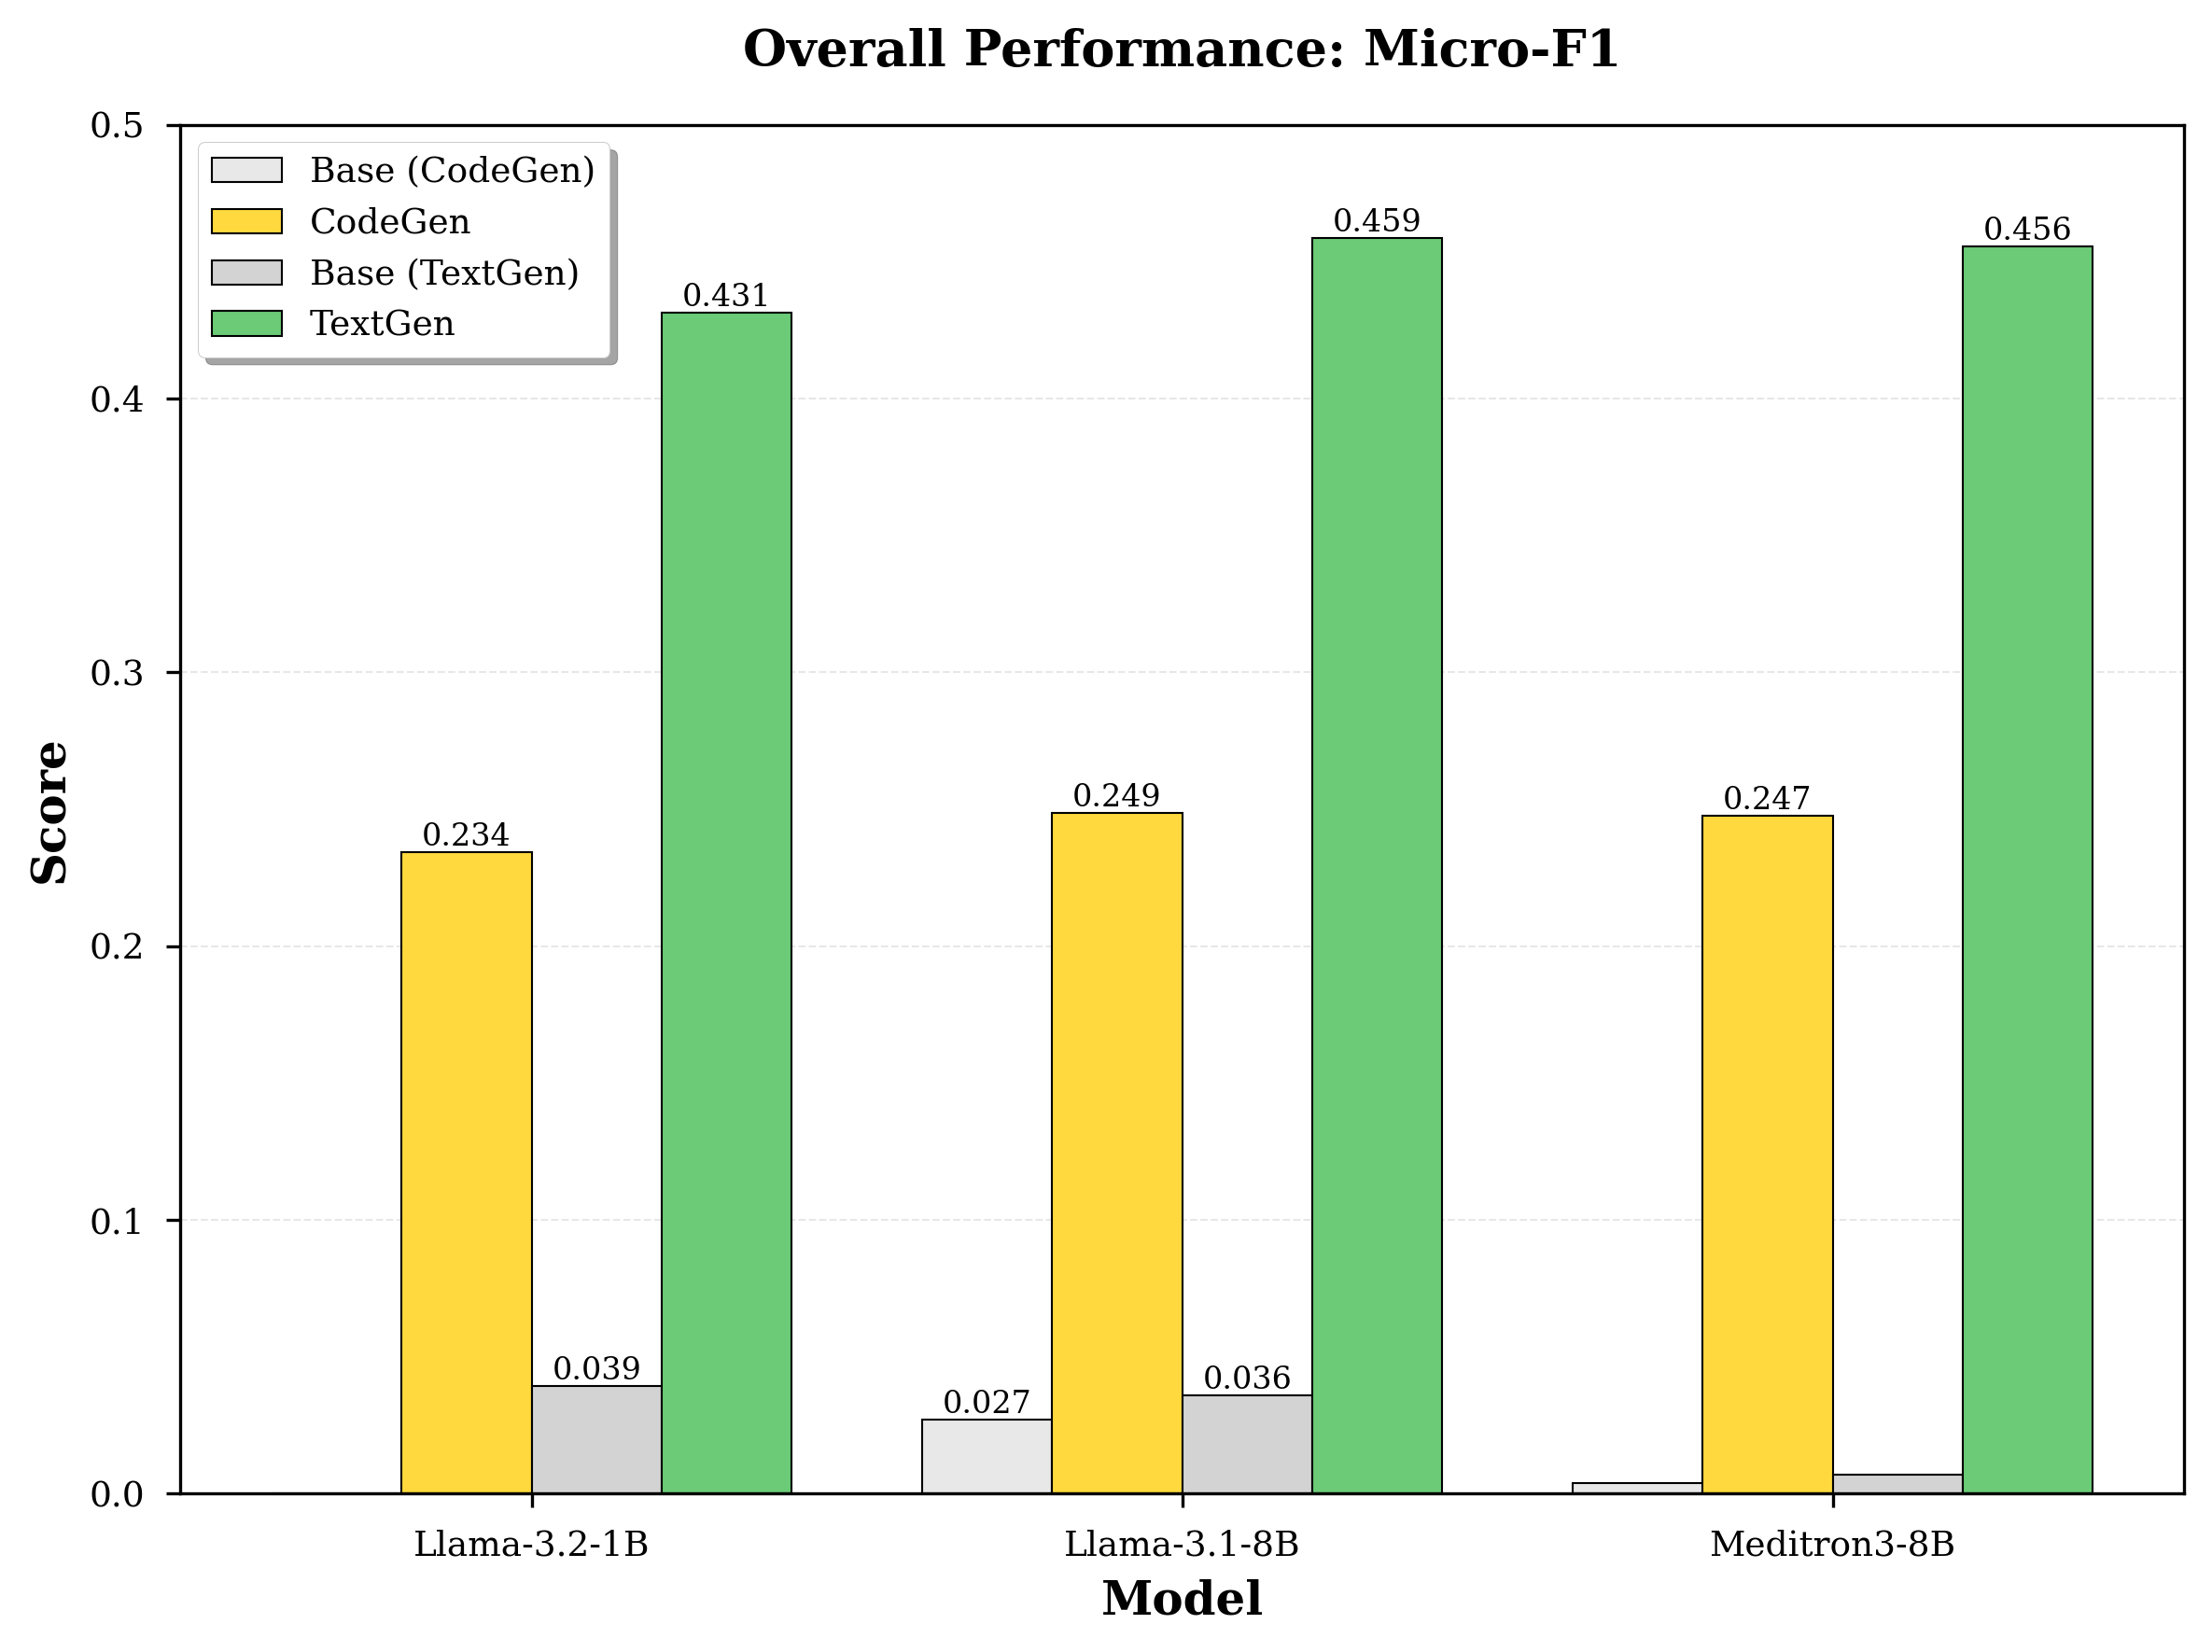
\includegraphics[width=\linewidth]{Images/Plots_thesis/overall_micro_f1.png}
%         \caption{Micro-F1}
%         \label{fig:task1-flat-microF1}
%     \end{subfigure}

%     \vspace{0.3cm}

%     % Bottom row: macro-averaged metrics
%     \begin{subfigure}{0.32\textwidth}
%         \centering
%         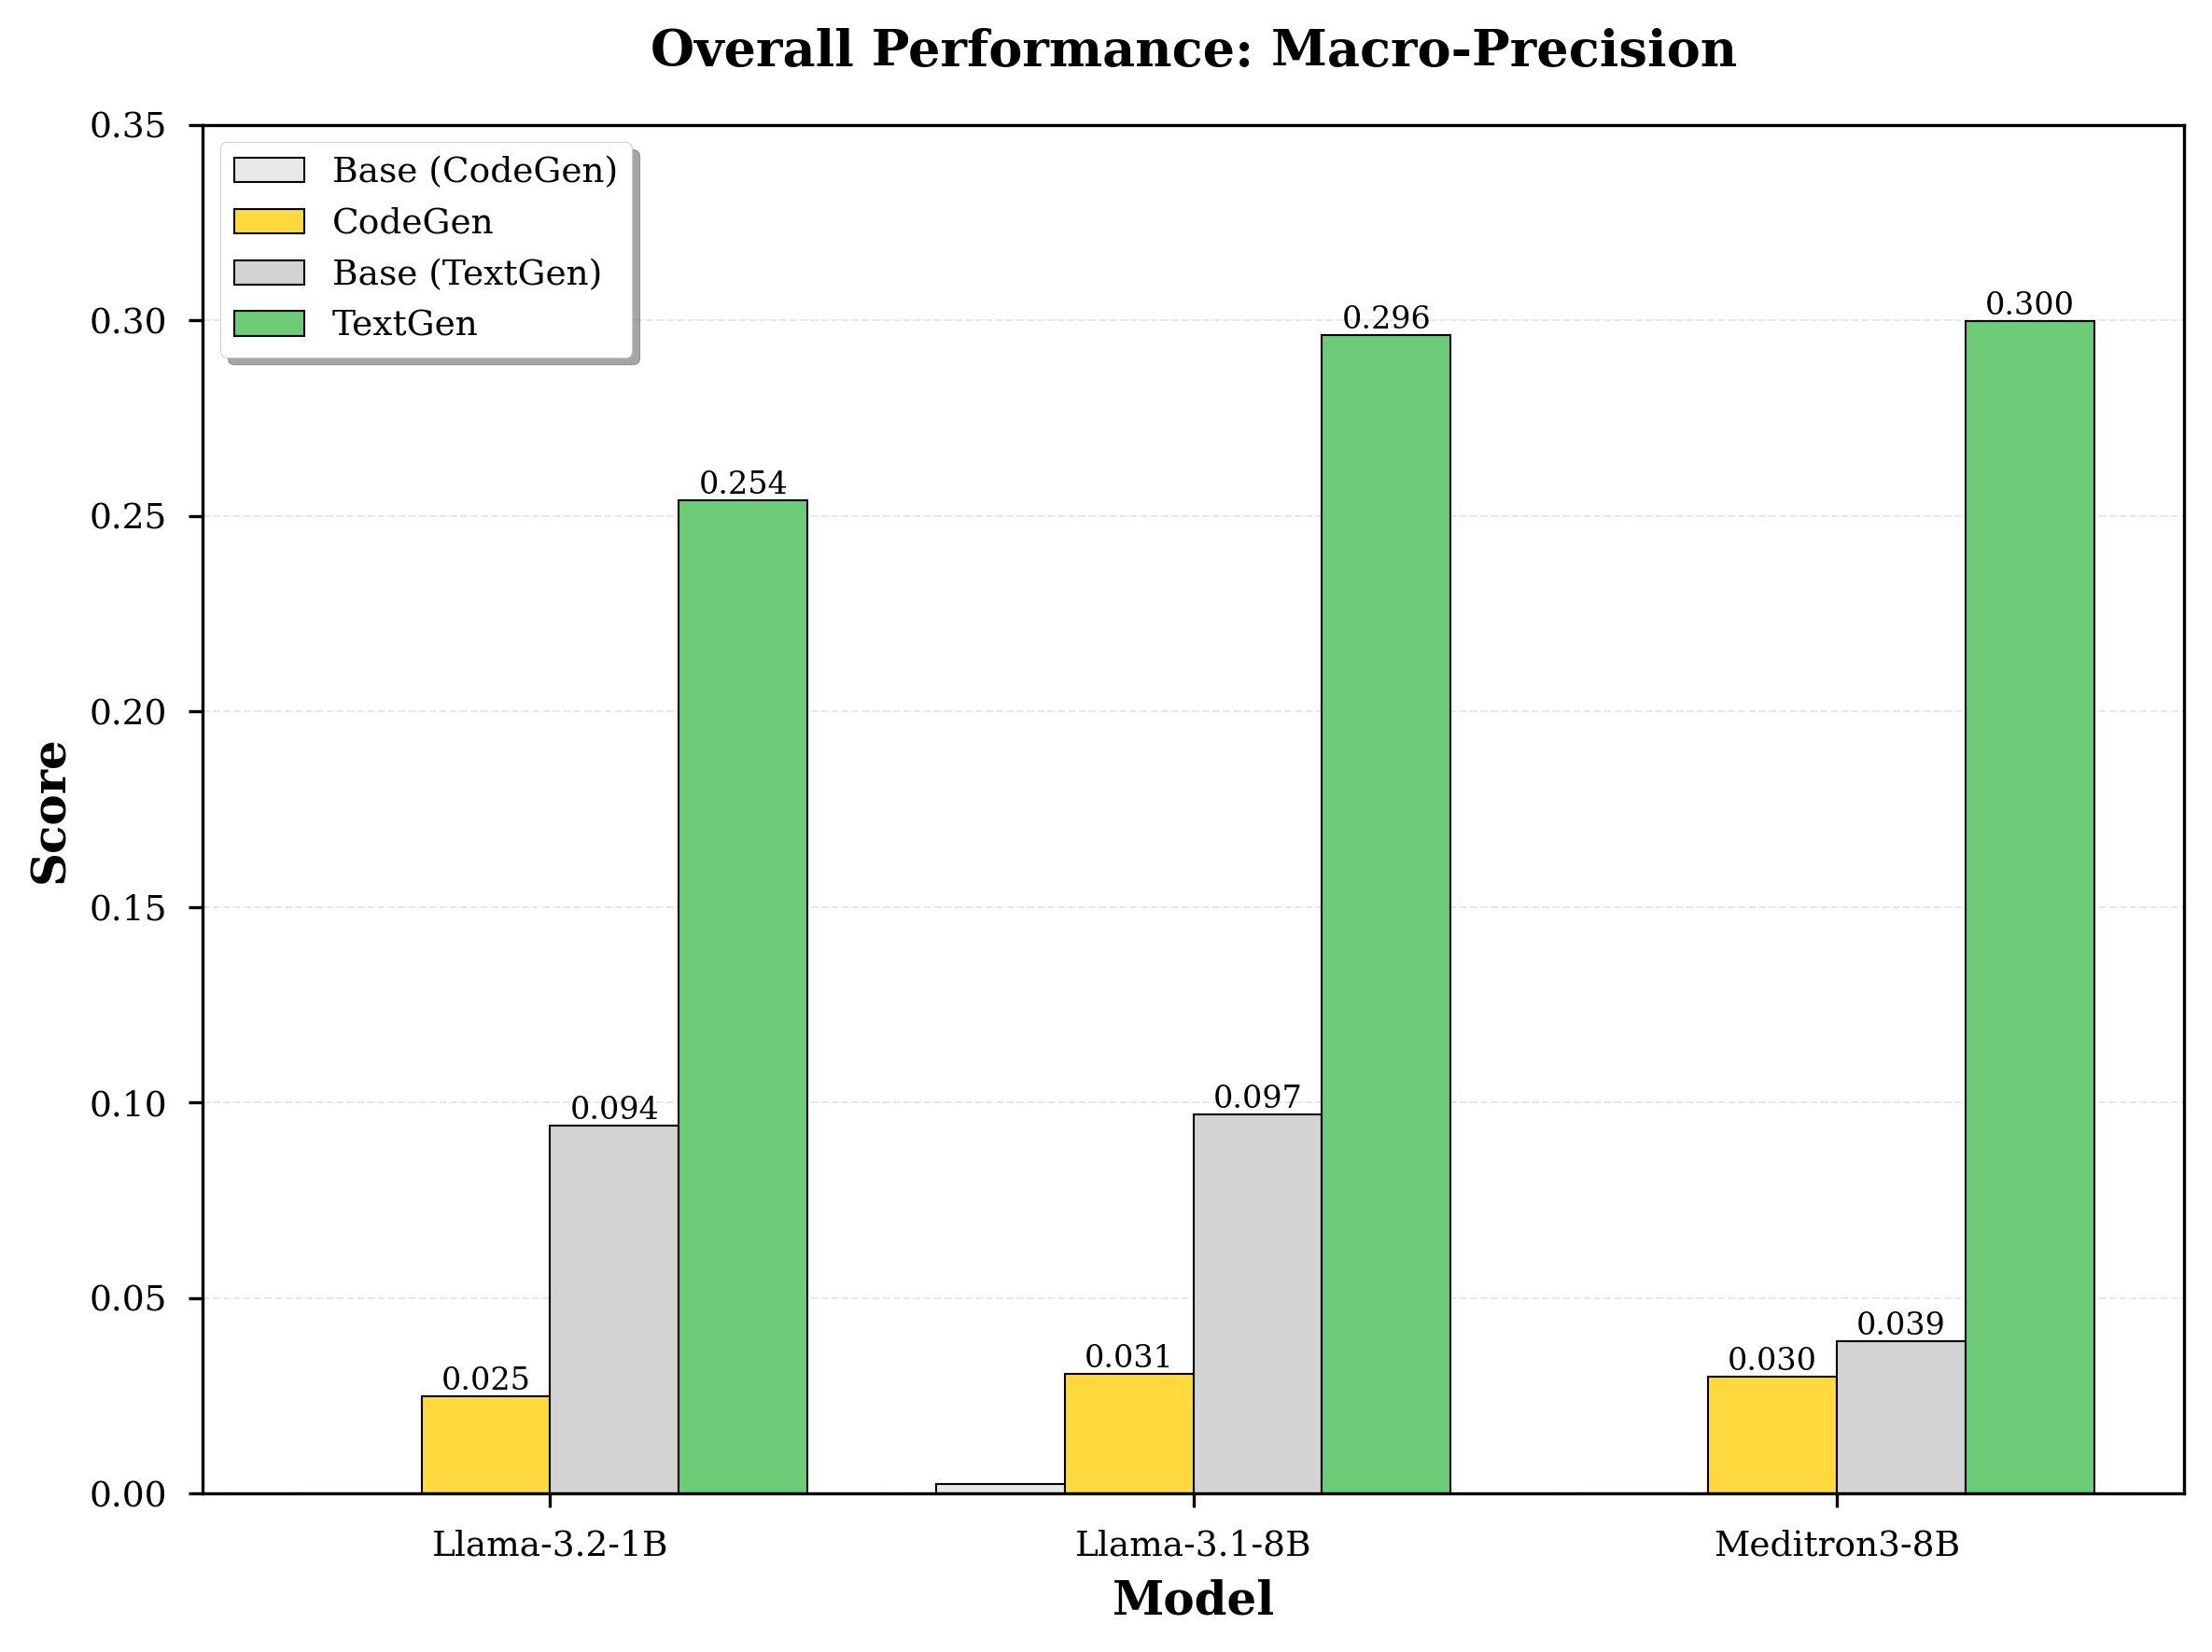
\includegraphics[width=\linewidth]{Images/Plots_thesis/overall_macro_precision.png}
%         \caption{Macro-Precision}
%         \label{fig:task1-flat-macroP}
%     \end{subfigure}\hfill
%     \begin{subfigure}{0.32\textwidth}
%         \centering
%         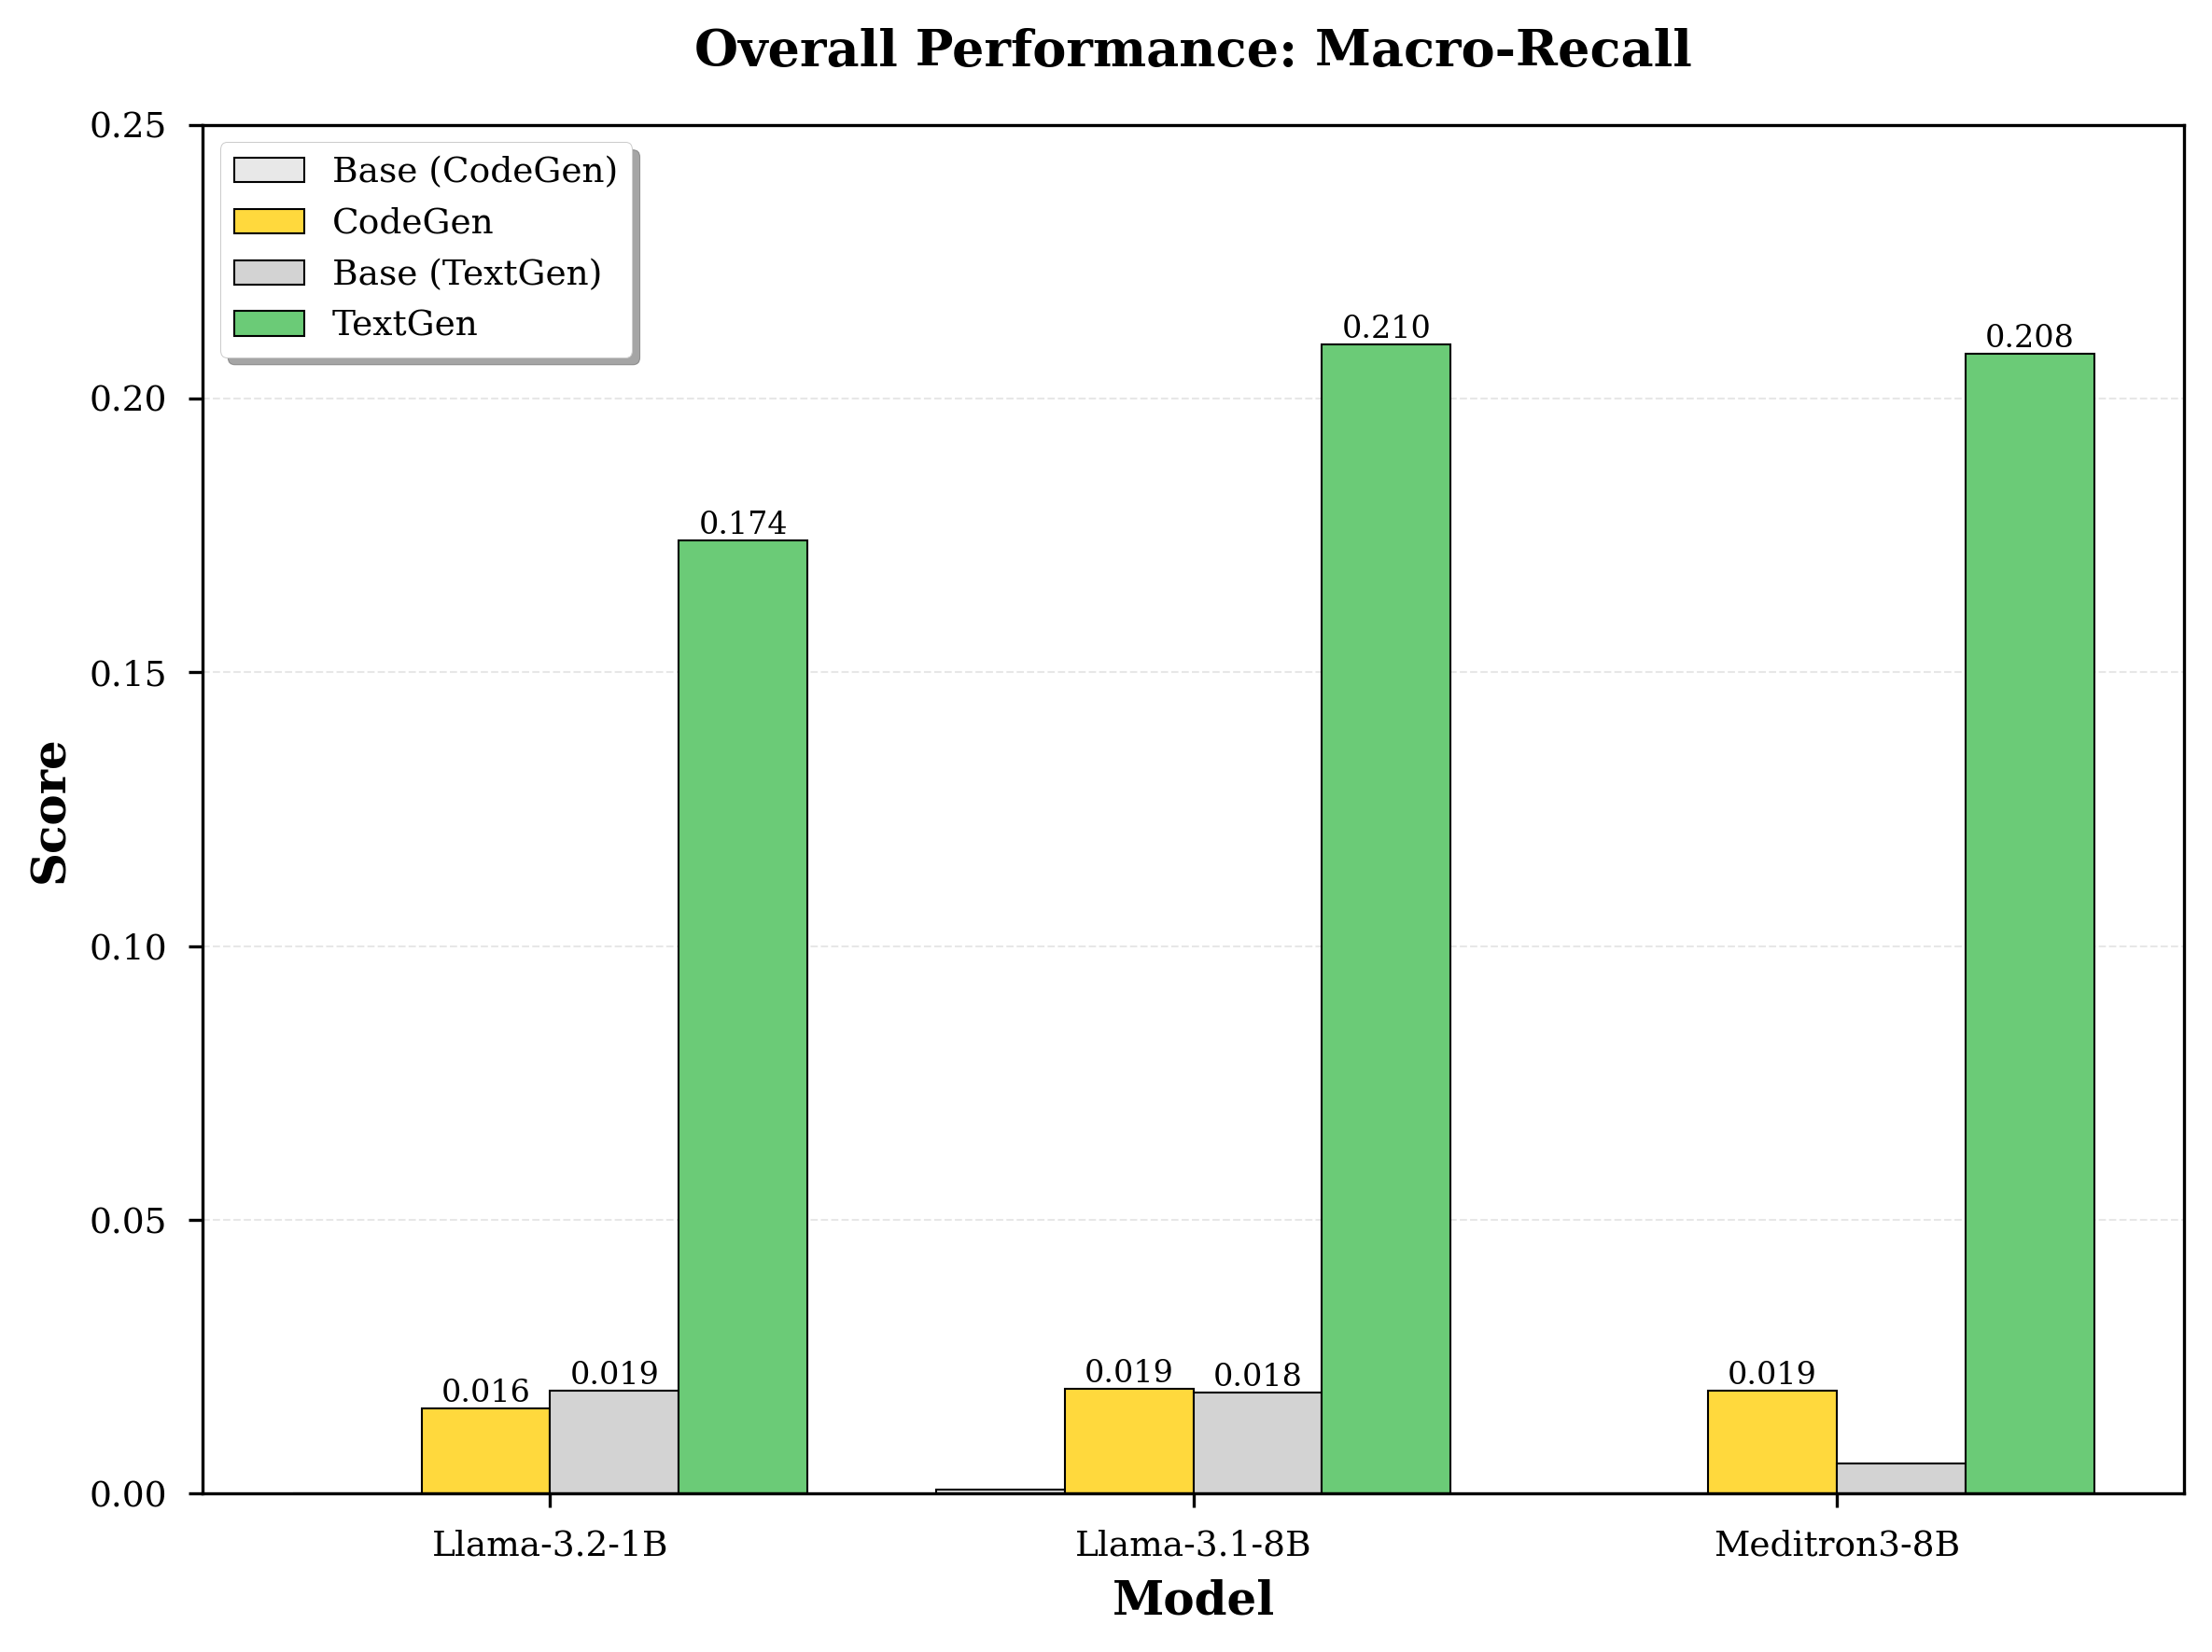
\includegraphics[width=\linewidth]{Images/Plots_thesis/overall_macro_recall.png}
%         \caption{Macro-Recall}
%         \label{fig:task1-flat-macroR}
%     \end{subfigure}\hfill
%     \begin{subfigure}{0.32\textwidth}
%         \centering
%         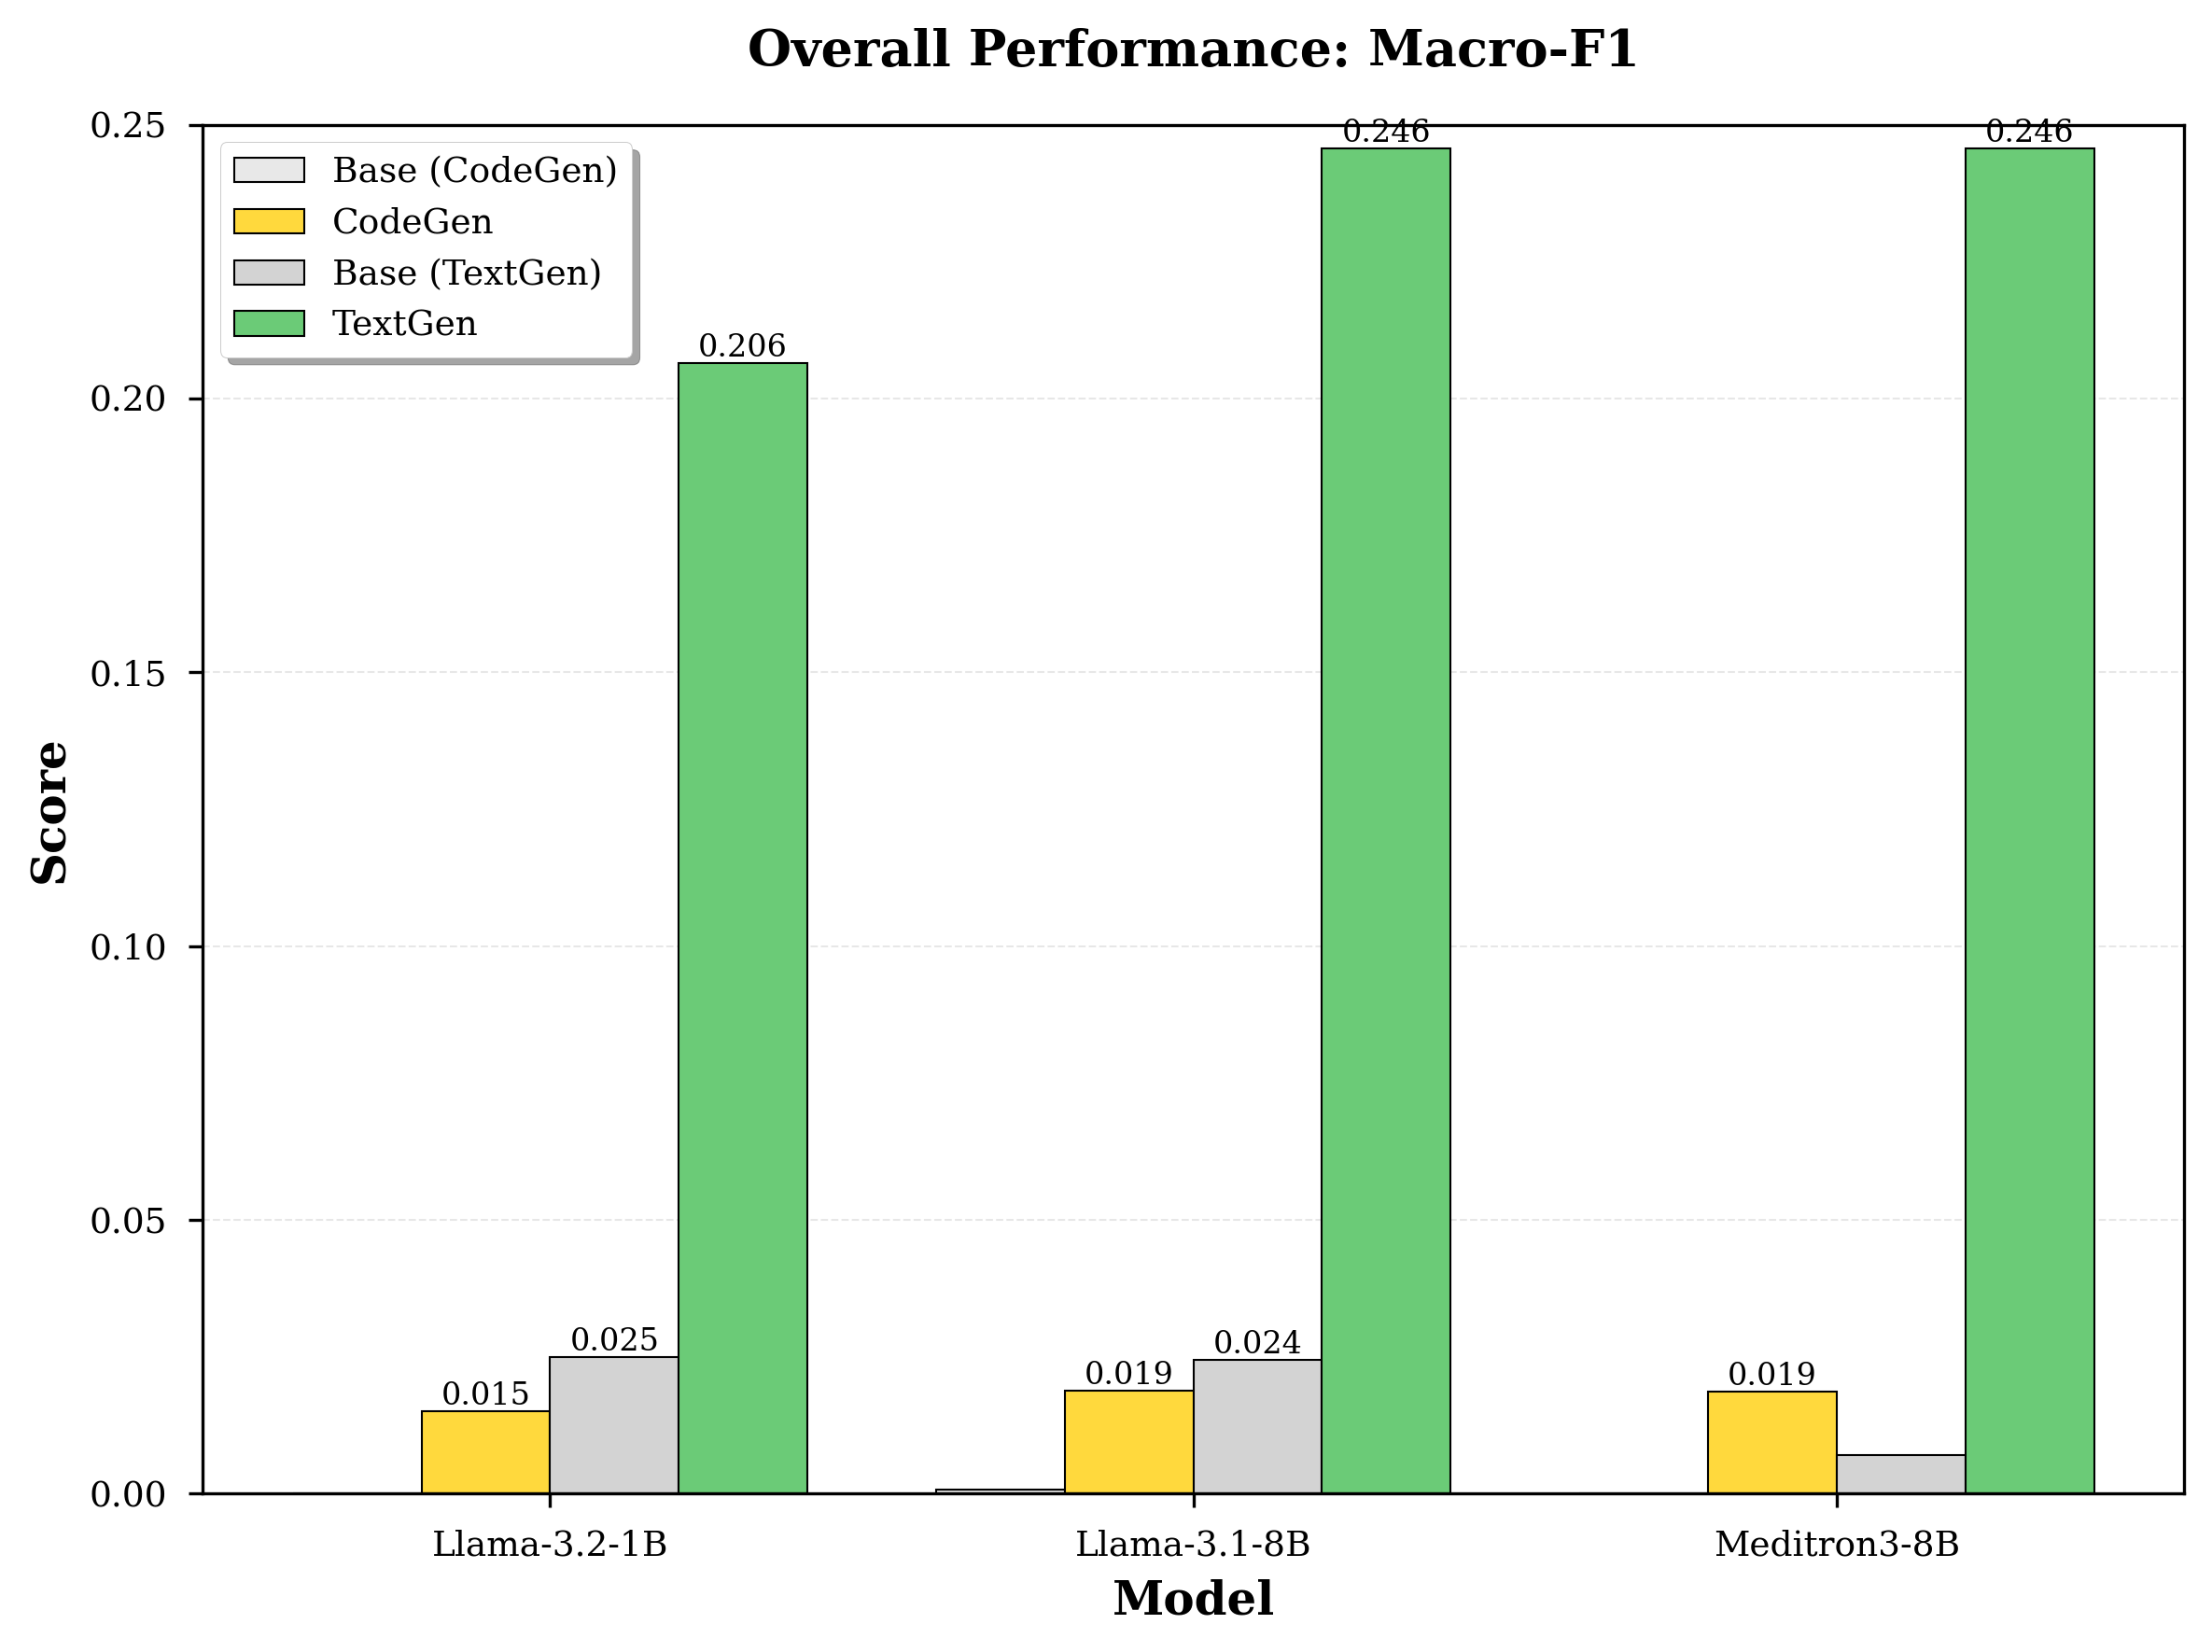
\includegraphics[width=\linewidth]{Images/Plots_thesis/overall_macro_f1.png}
%         \caption{Macro-F1}
%         \label{fig:task1-flat-macroF1}
%     \end{subfigure}

%     \caption{Task~1: flat (full-code) evaluation. Micro- and macro-averaged precision, recall, and F1 for \textbf{Base} (raw backbones), \textbf{CodeGen} (fine-tuned direct ICD-9 generation), and \textbf{TextGen} (fine-tuned diagnosis-term generation + semantic mapping) across all backbones.}
%     \label{fig:task1-flat-metrics}
% \end{figure}

% Overall, Table~\ref{tab:task1-all-methods-flat} and Figure~\ref{fig:task1-flat-metrics} establish a clear ranking:
% \[
% \text{Base} \;\ll\; \text{CodeGen} \;<\; \text{TextGen},
% \]
% with stronger performance for 8B backbones than 1B. These findings justify using \textbf{TextGen} as the default pipeline for the knowledge-augmentation experiments.

% % ============================================================
% \subsection{Hierarchical Evaluation at the Parent-Code Level}
% \label{subsec:results-task1-hierarchical}

% Flat ICD-9 evaluation assigns full penalty to any mismatch at the exact code level, even if the predicted code falls under the correct diagnostic family. To quantify clinically meaningful ``near misses'', we compute \emph{parent-level} metrics (Section~\ref{subsec:hierarchical-metrics}), where codes are collapsed to their three-digit parent categories.

% Table~\ref{tab:task1-parent-metrics} shows a consistent increase in F1 relative to full-code evaluation, indicating that many errors occur within the correct disease family (e.g., predicting a related subtype rather than a completely unrelated diagnosis). TextGen retains a clear advantage at the parent level, implying its gains reflect improved clinical alignment rather than merely better formatting.

% \begin{table}[t]
%     \centering
%     \caption{Task~1 hierarchical evaluation at the ICD-9 parent (three-digit) level. Metrics computed after collapsing codes to parent categories (test set).}
%     \label{tab:task1-parent-metrics}
%     \begin{tabular}{llcc}
%         \toprule
%         \textbf{Backbone} & \textbf{Method} &
%         \textbf{Parent micro-F1} &
%         \textbf{Parent macro-F1} \\
%         \midrule
%         \multirow{4}{*}{Llama-3.2-1B} 
%             & Base (no FT) - Direct codes   & 0.0014 & 0.0007 \\
%             & CodeGen        & 0.4687 & 0.2572 \\
%             & Base (no FT) - Free Text  & 0.0677 & 0.0387  \\
%             & TextGen        & \textbf{0.4800} & \textbf{0.2732} \\
%         \midrule
%         \multirow{4}{*}{Llama-3.1-8B} 
%             & Base (no FT) - Direct codes   & 0.0953 & 0.0281 \\
%             & CodeGen        & 0.4814 & 0.2973 \\
%             & Base (no FT) - Free Text  & 0.0618 & 0.0378  \\
%             & TextGen        & \textbf{0.5388} & \textbf{0.3459} \\
%         \midrule
%         \multirow{4}{*}{Meditron-8B} 
%             & Base (no FT) - Direct codes   & 0.0083 & 0.0015 \\
%             & CodeGen        & 0.4771 & 0.2935 \\
%             & Base (no FT) - Free Text  & 0.0135 & 0.0111  \\
%             & TextGen        & \textbf{0.5364} & \textbf{0.3418} \\
%         \bottomrule
%     \end{tabular}
% \end{table}

% % --- KEEP THESE IMAGES EXACTLY (as requested) ---
% \begin{figure}[t]
%     \centering
%     % Top row: micro-averaged parent metrics
%     \begin{subfigure}{0.32\textwidth}
%         \centering
%         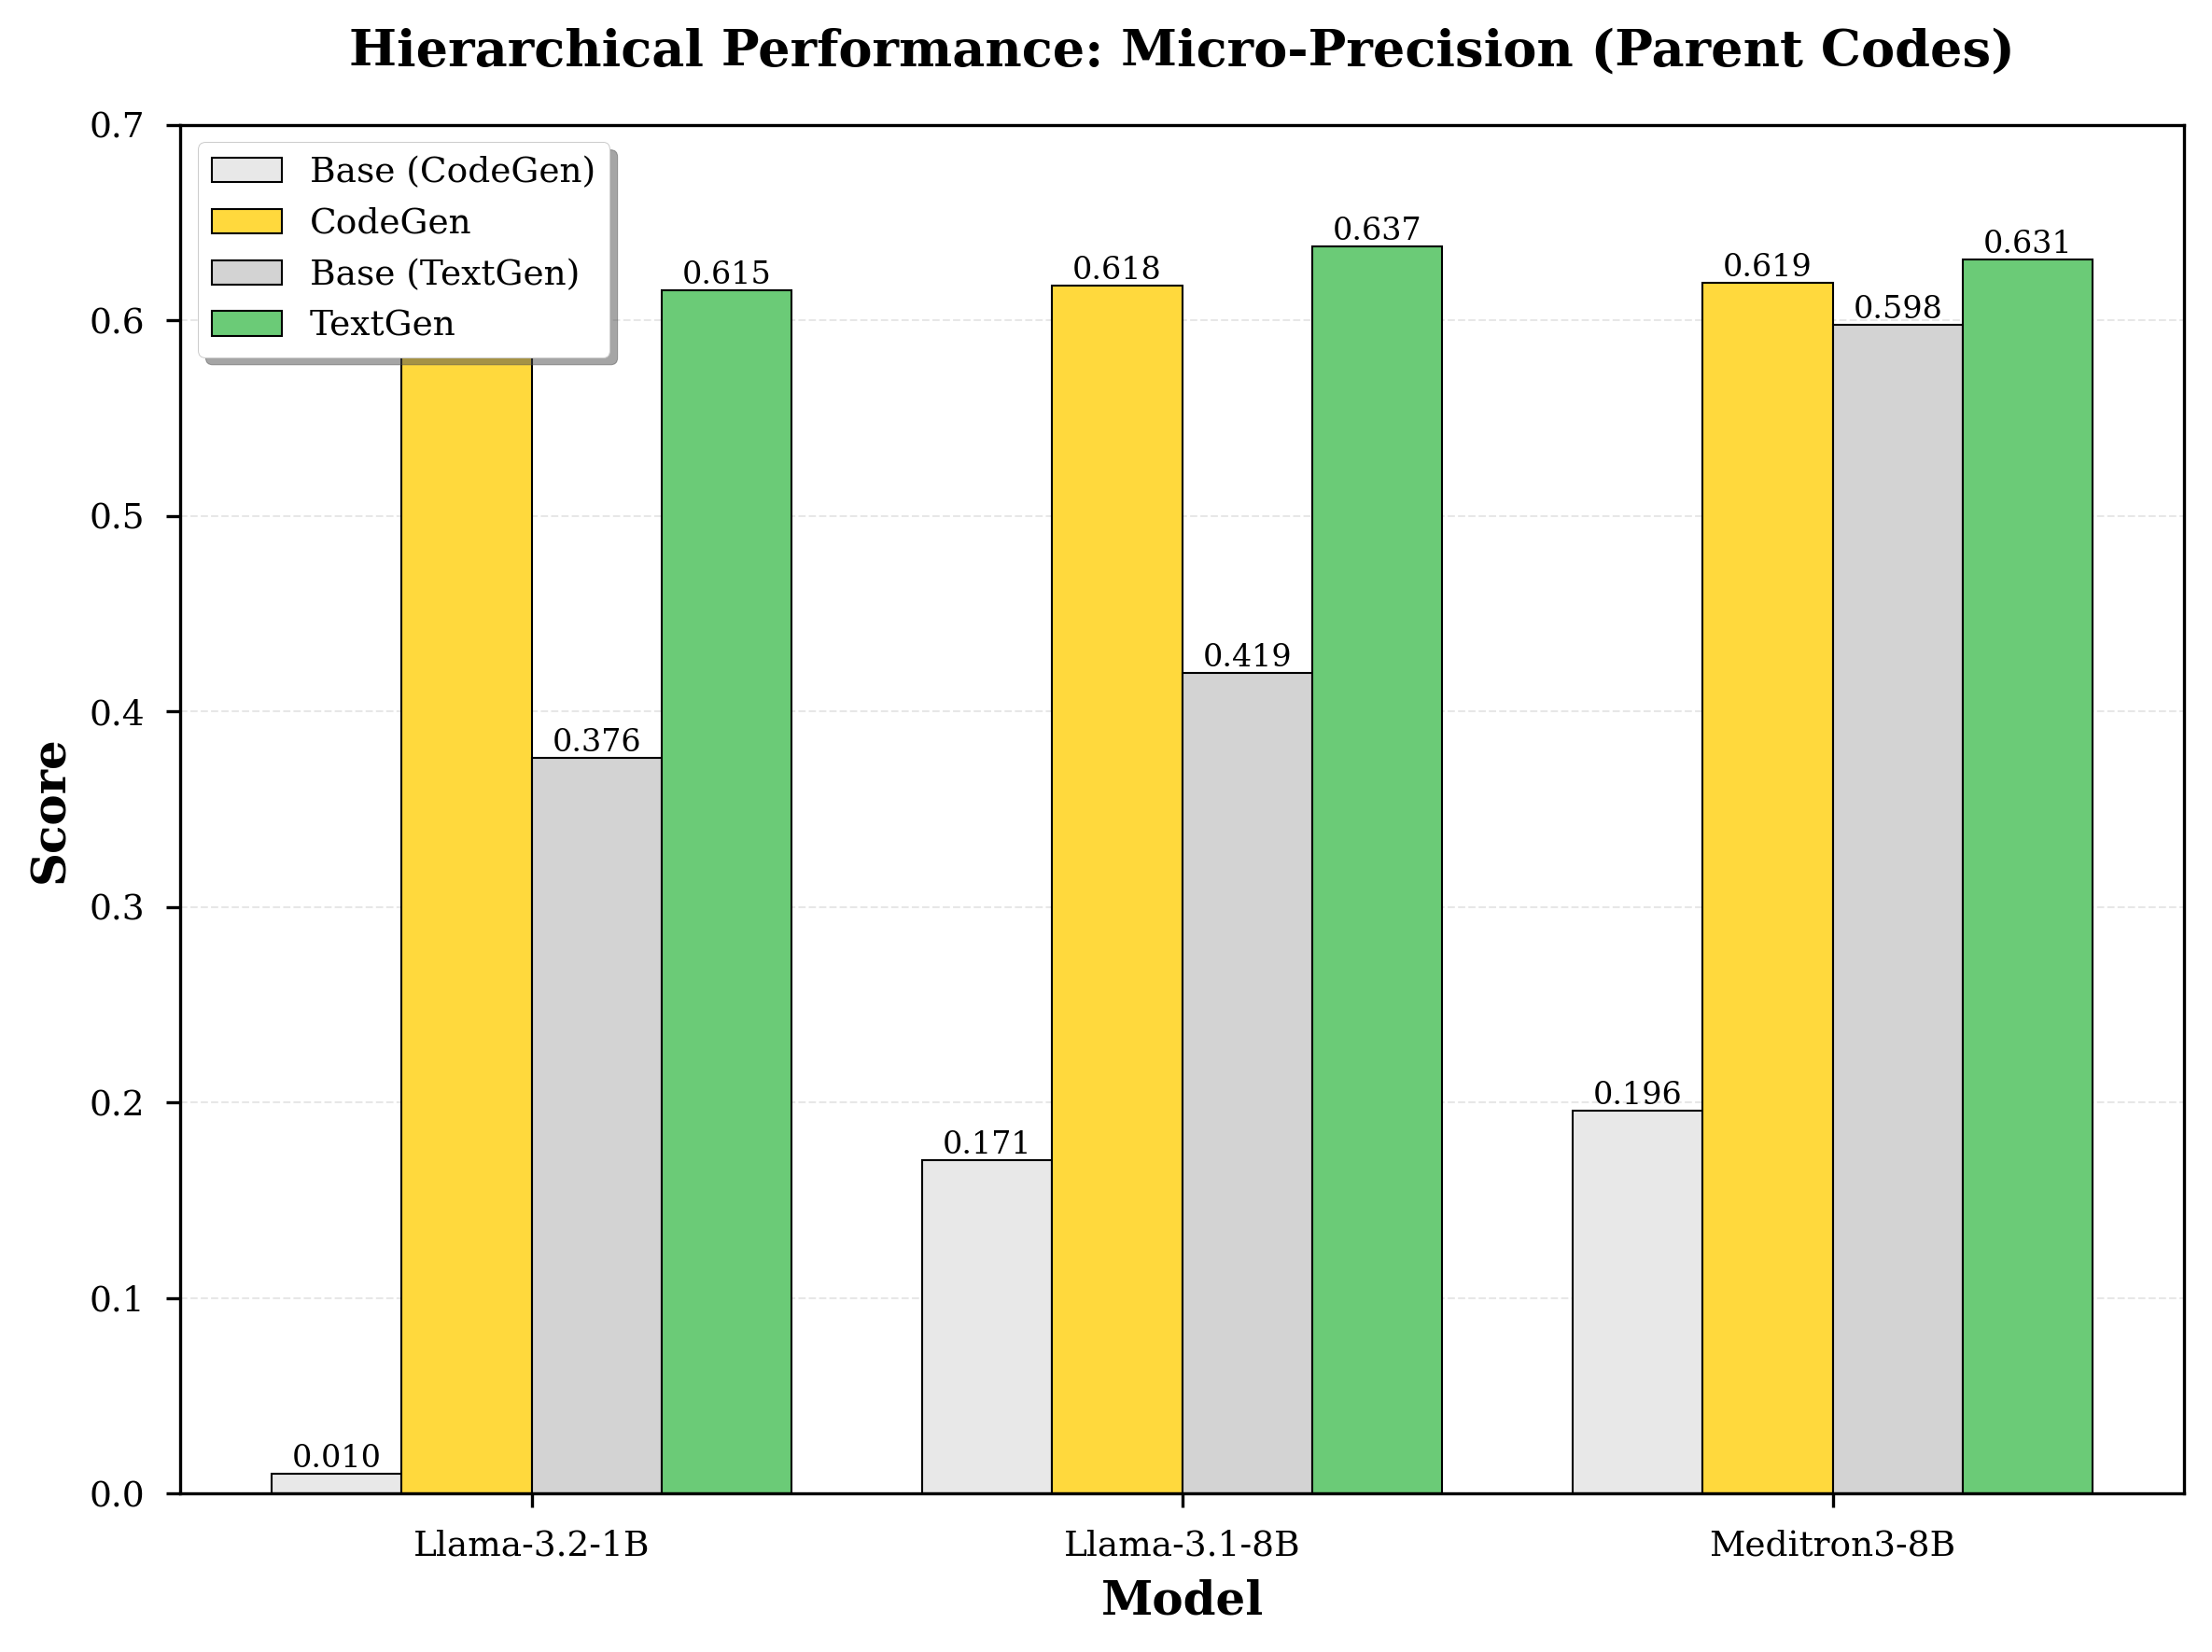
\includegraphics[width=\linewidth]{Images/Plots_thesis/parent_micro_precision.png}
%         \caption{Parent micro-Precision}
%         \label{fig:task1-parent-microP}
%     \end{subfigure}\hfill
%     \begin{subfigure}{0.32\textwidth}
%         \centering
%         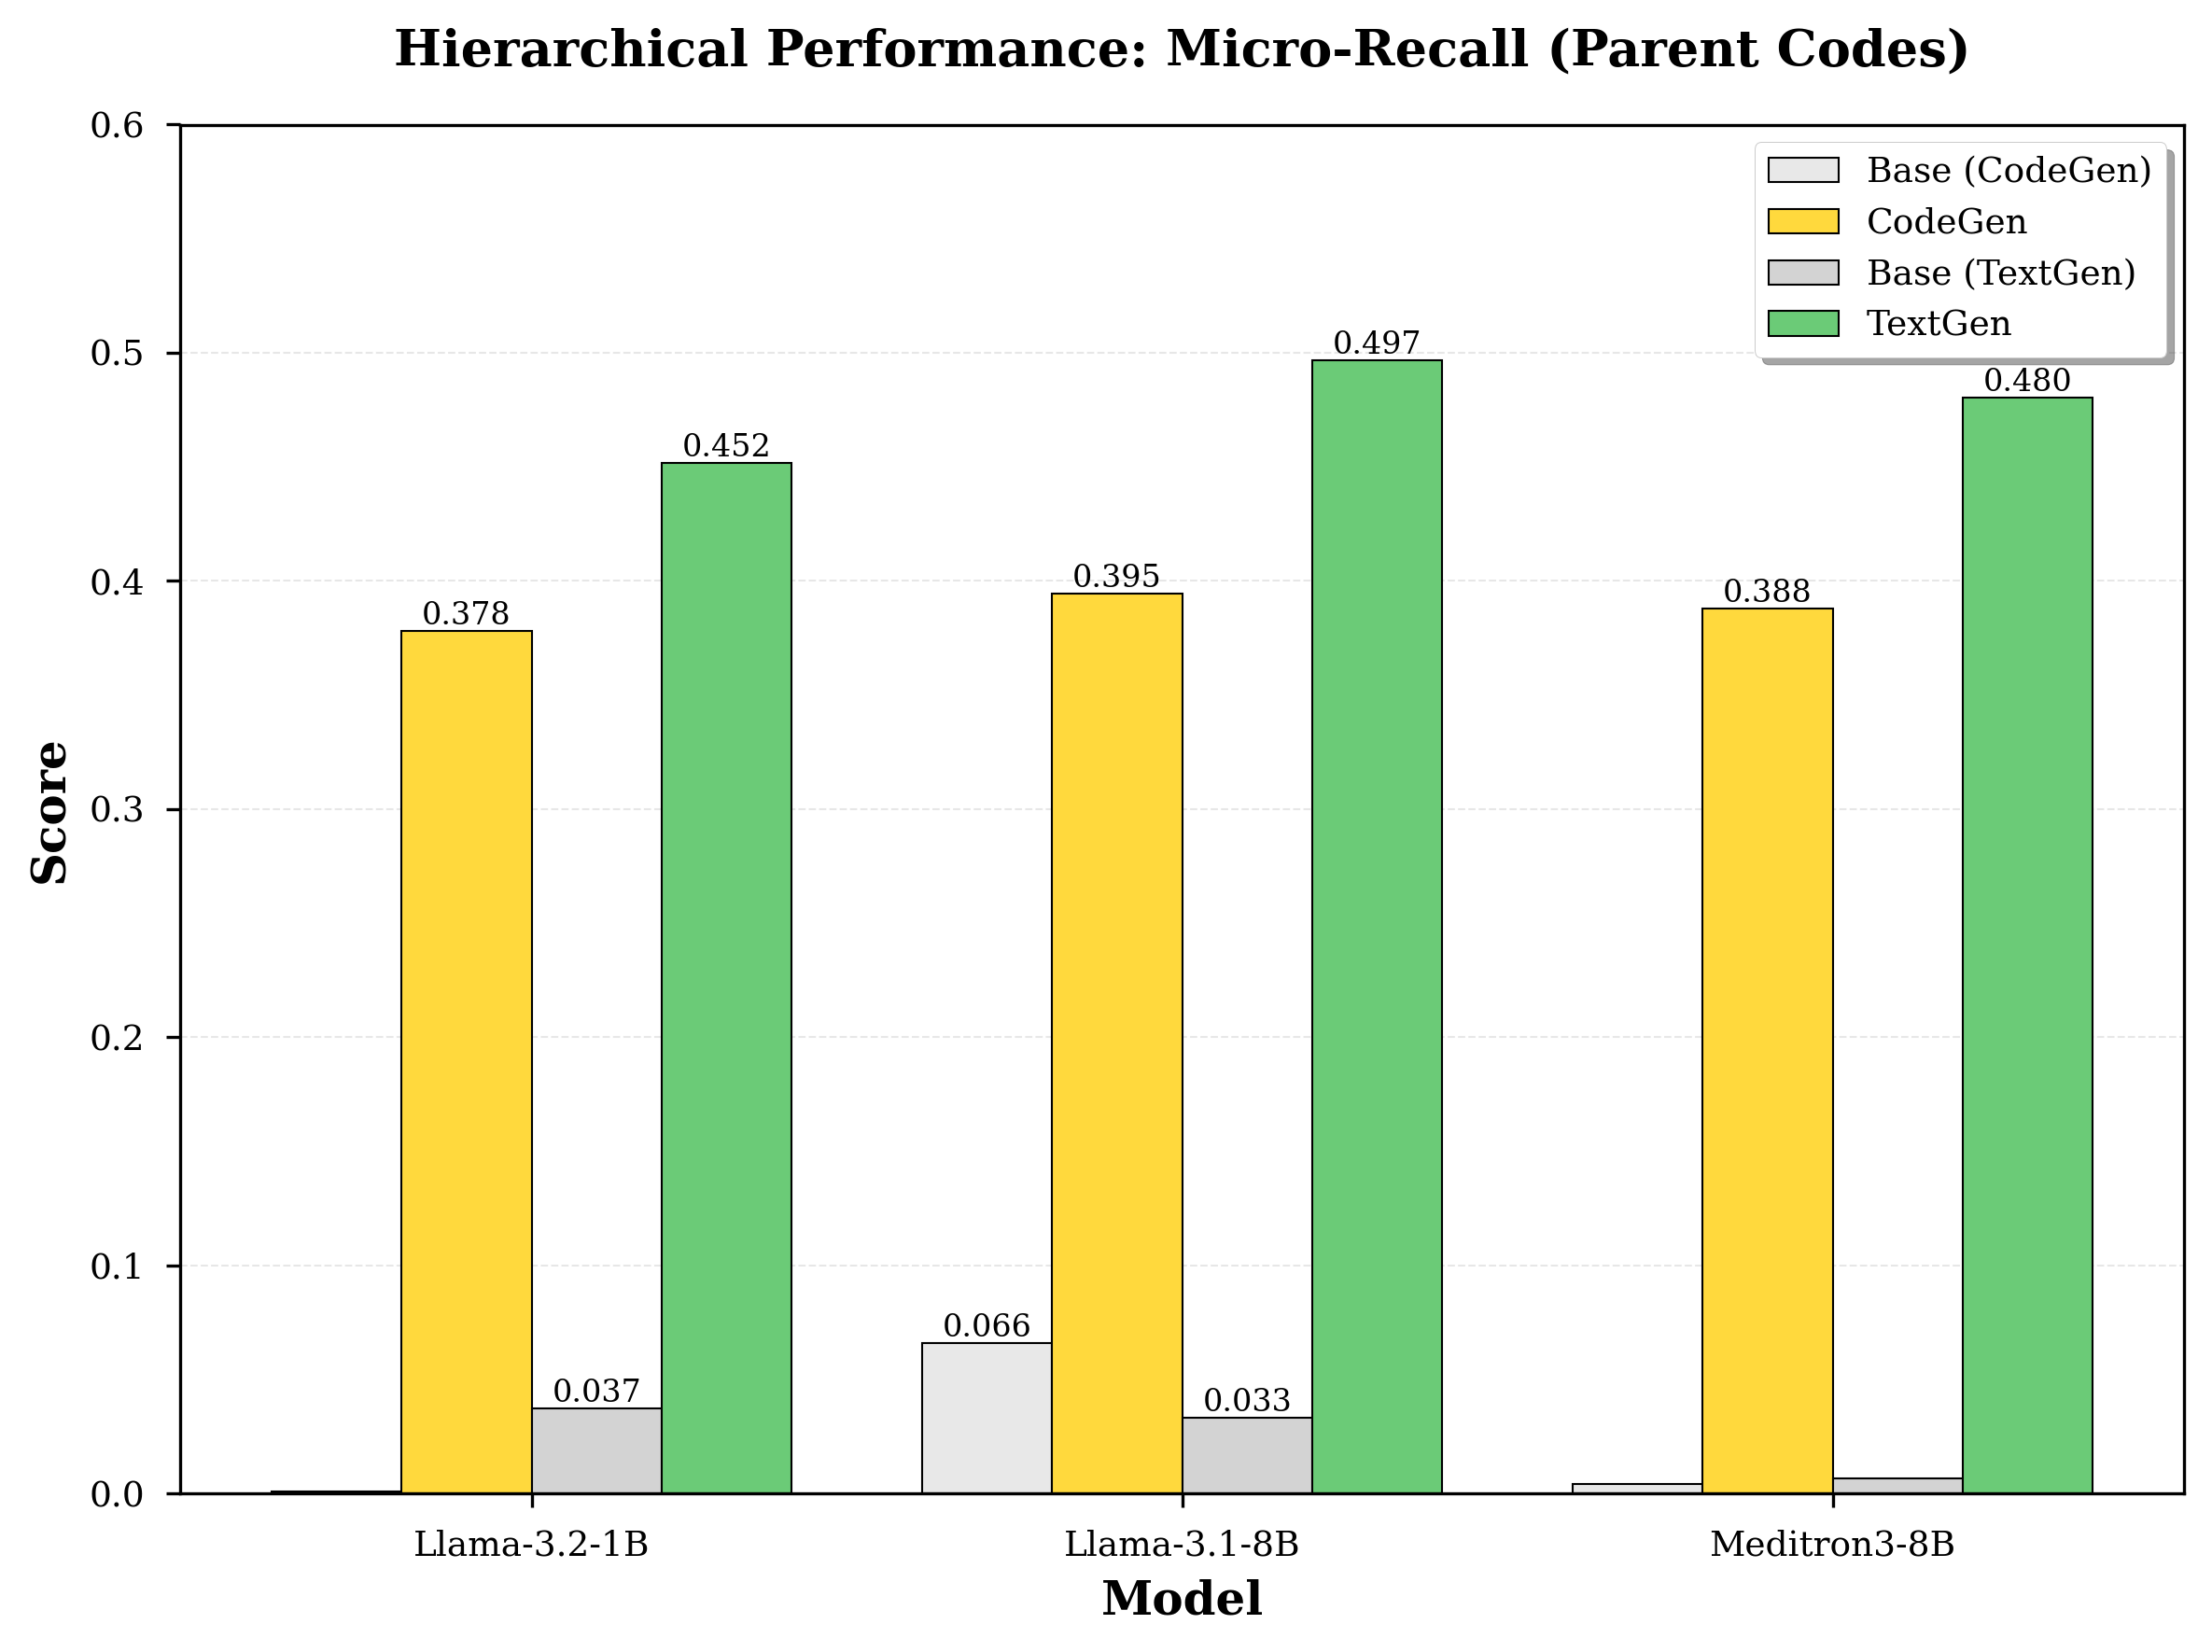
\includegraphics[width=\linewidth]{Images/Plots_thesis/parent_micro_recall.png}
%         \caption{Parent micro-Recall}
%         \label{fig:task1-parent-microR}
%     \end{subfigure}\hfill
%     \begin{subfigure}{0.32\textwidth}
%         \centering
%         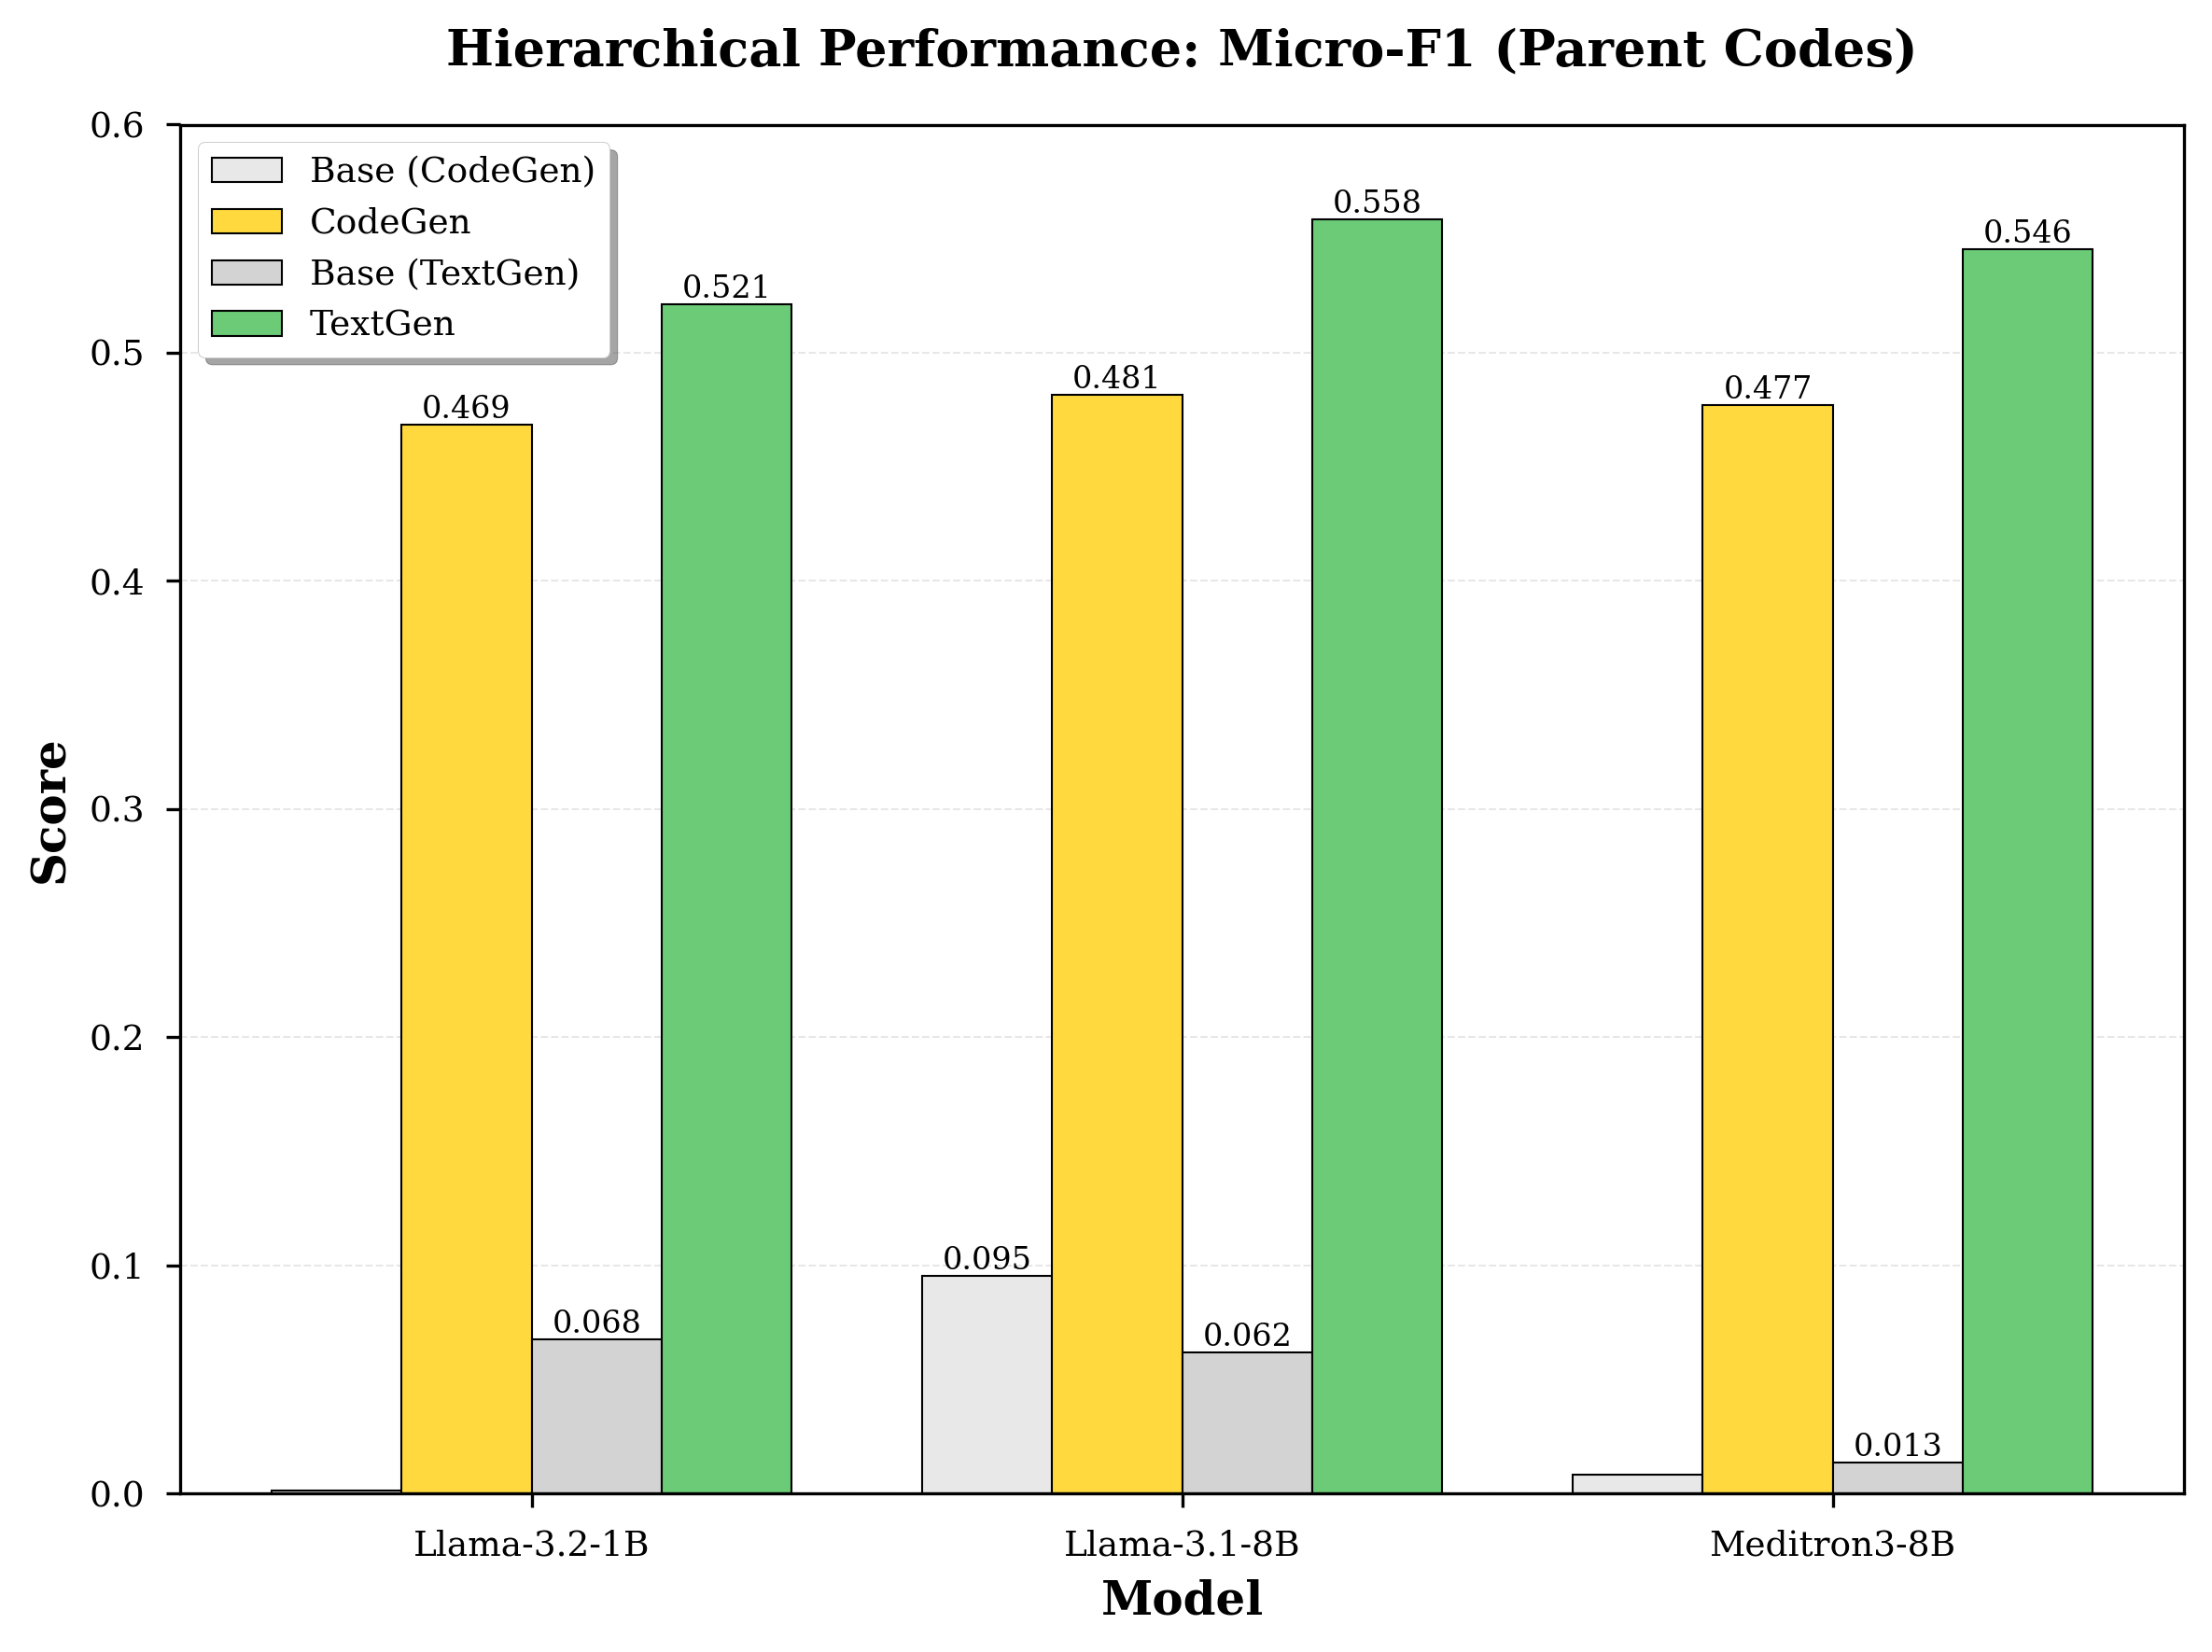
\includegraphics[width=\linewidth]{Images/Plots_thesis/parent_micro_f1.png}
%         \caption{Parent micro-F1}
%         \label{fig:task1-parent-microF1}
%     \end{subfigure}

%     \vspace{0.3cm}

%     % Bottom row: macro-averaged parent metrics
%     \begin{subfigure}{0.32\textwidth}
%         \centering
%         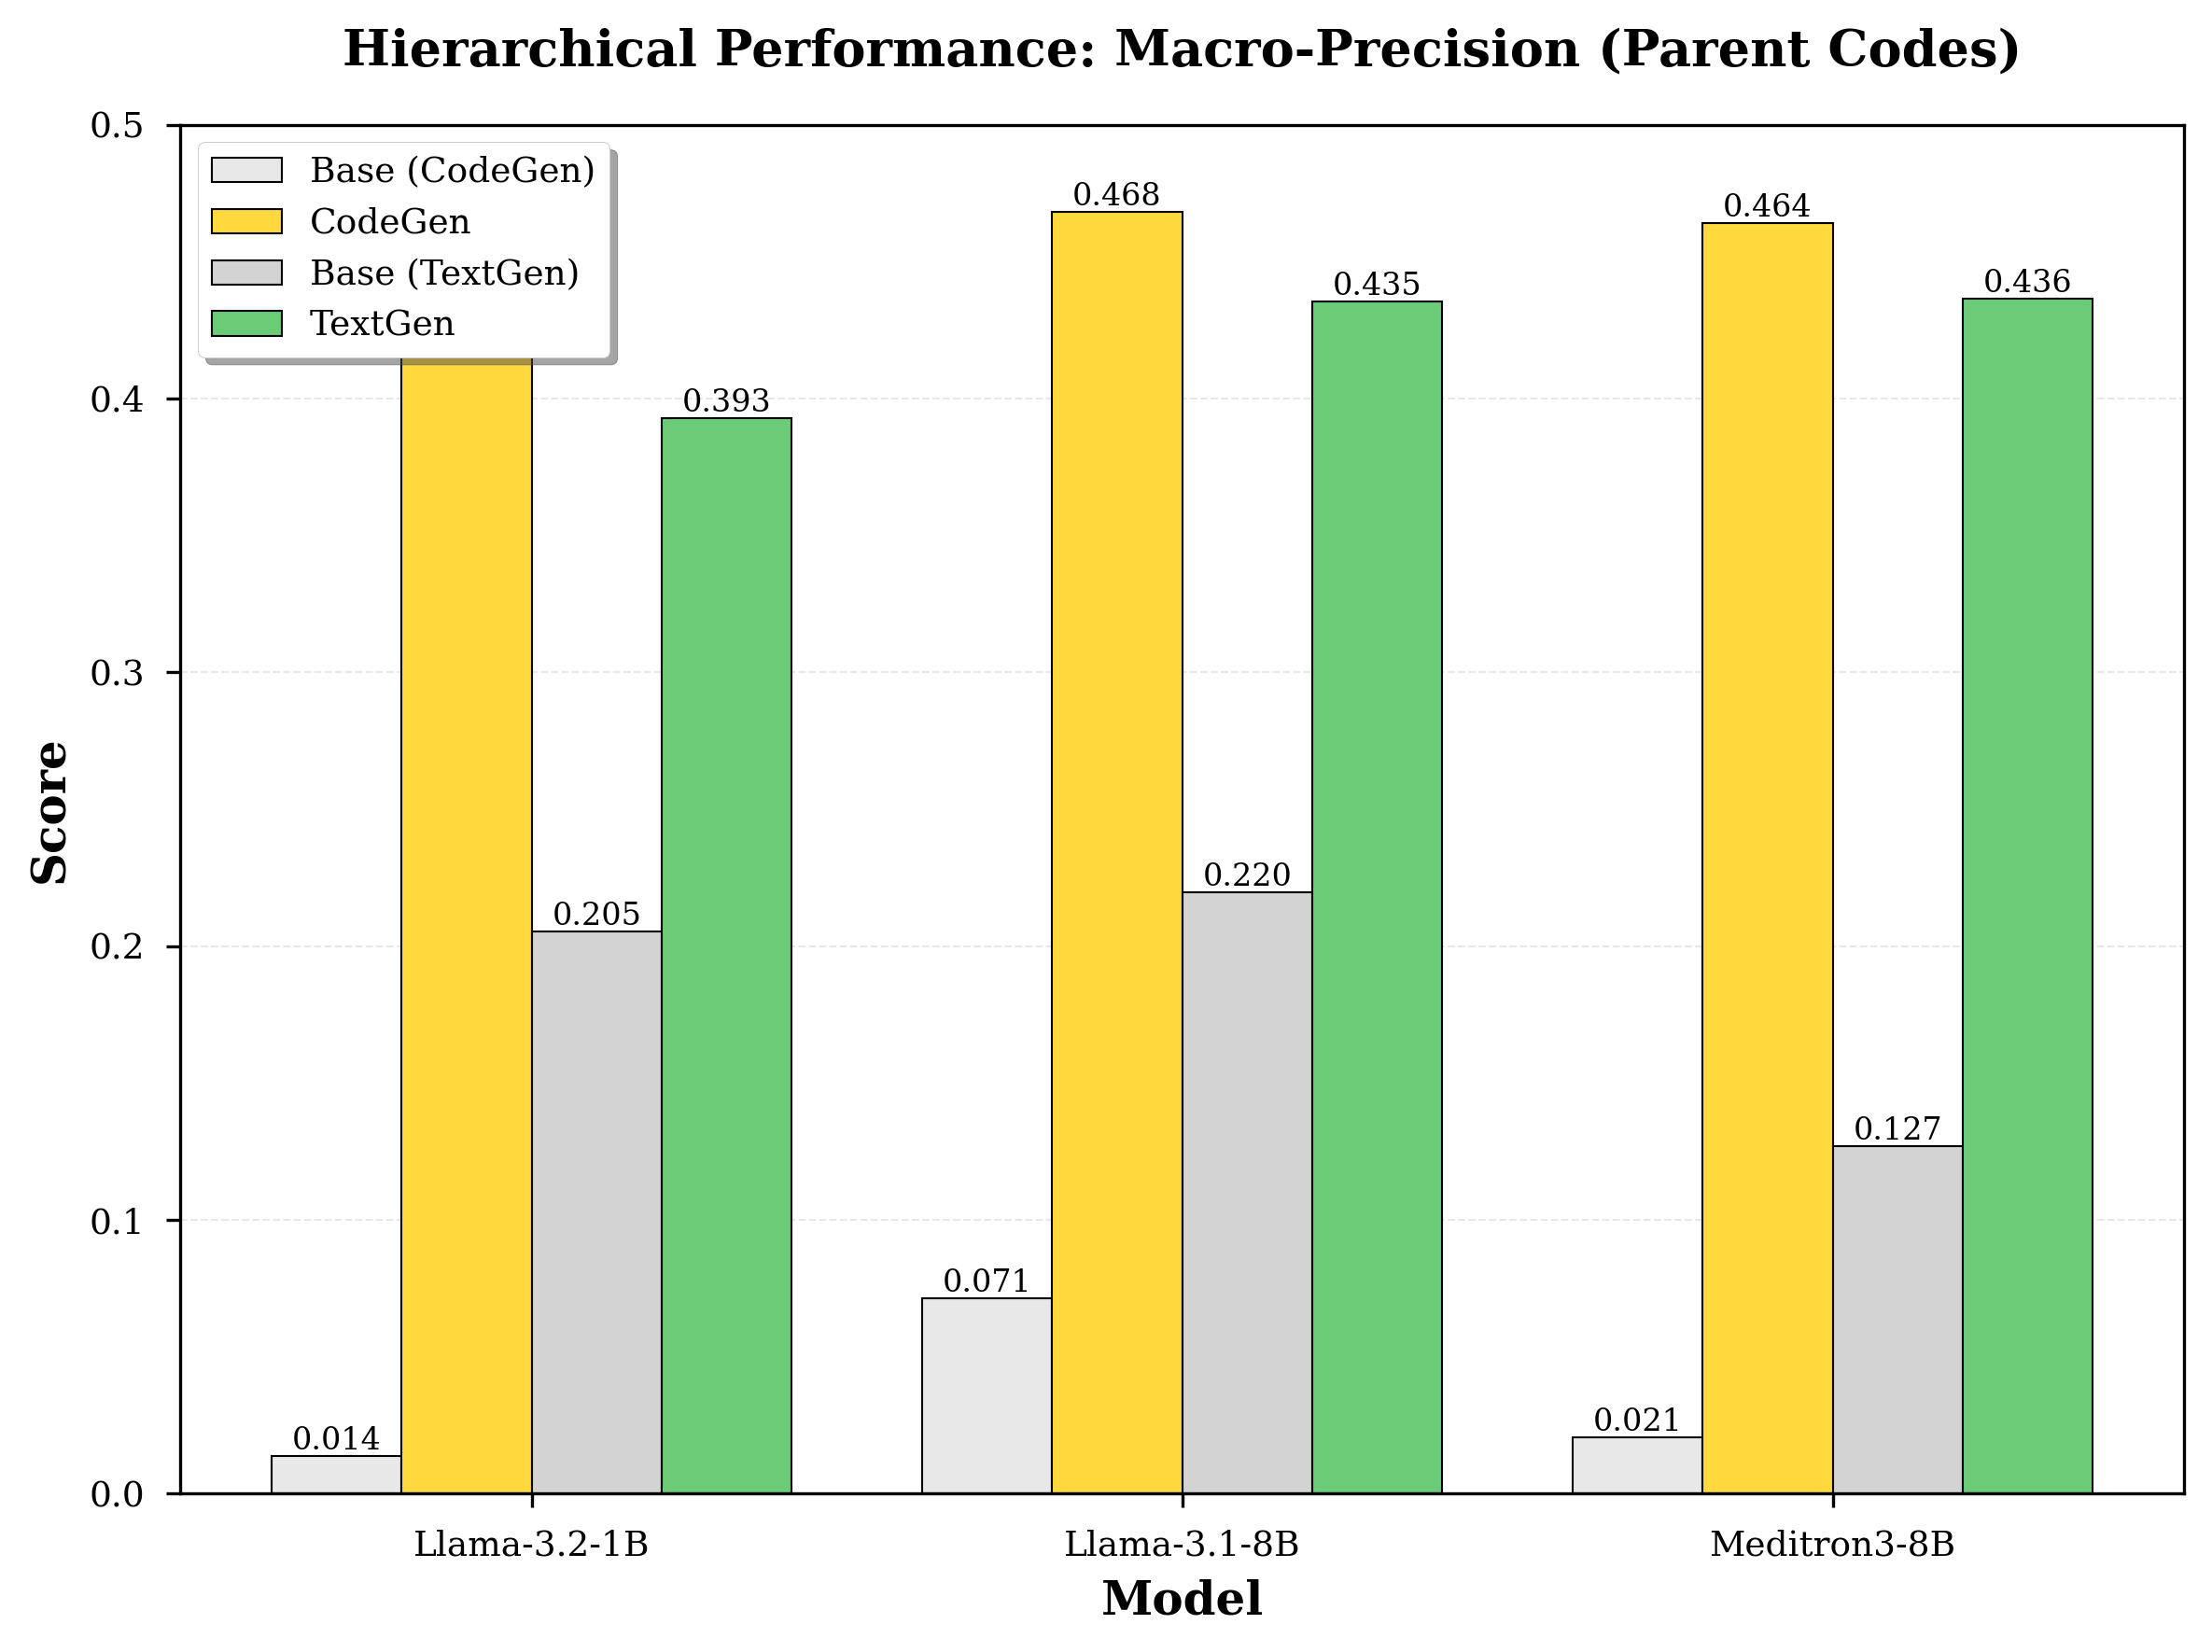
\includegraphics[width=\linewidth]{Images/Plots_thesis/parent_macro_precision.png}
%         \caption{Parent macro-Precision}
%         \label{fig:task1-parent-macroP}
%     \end{subfigure}\hfill
%     \begin{subfigure}{0.32\textwidth}
%         \centering
%         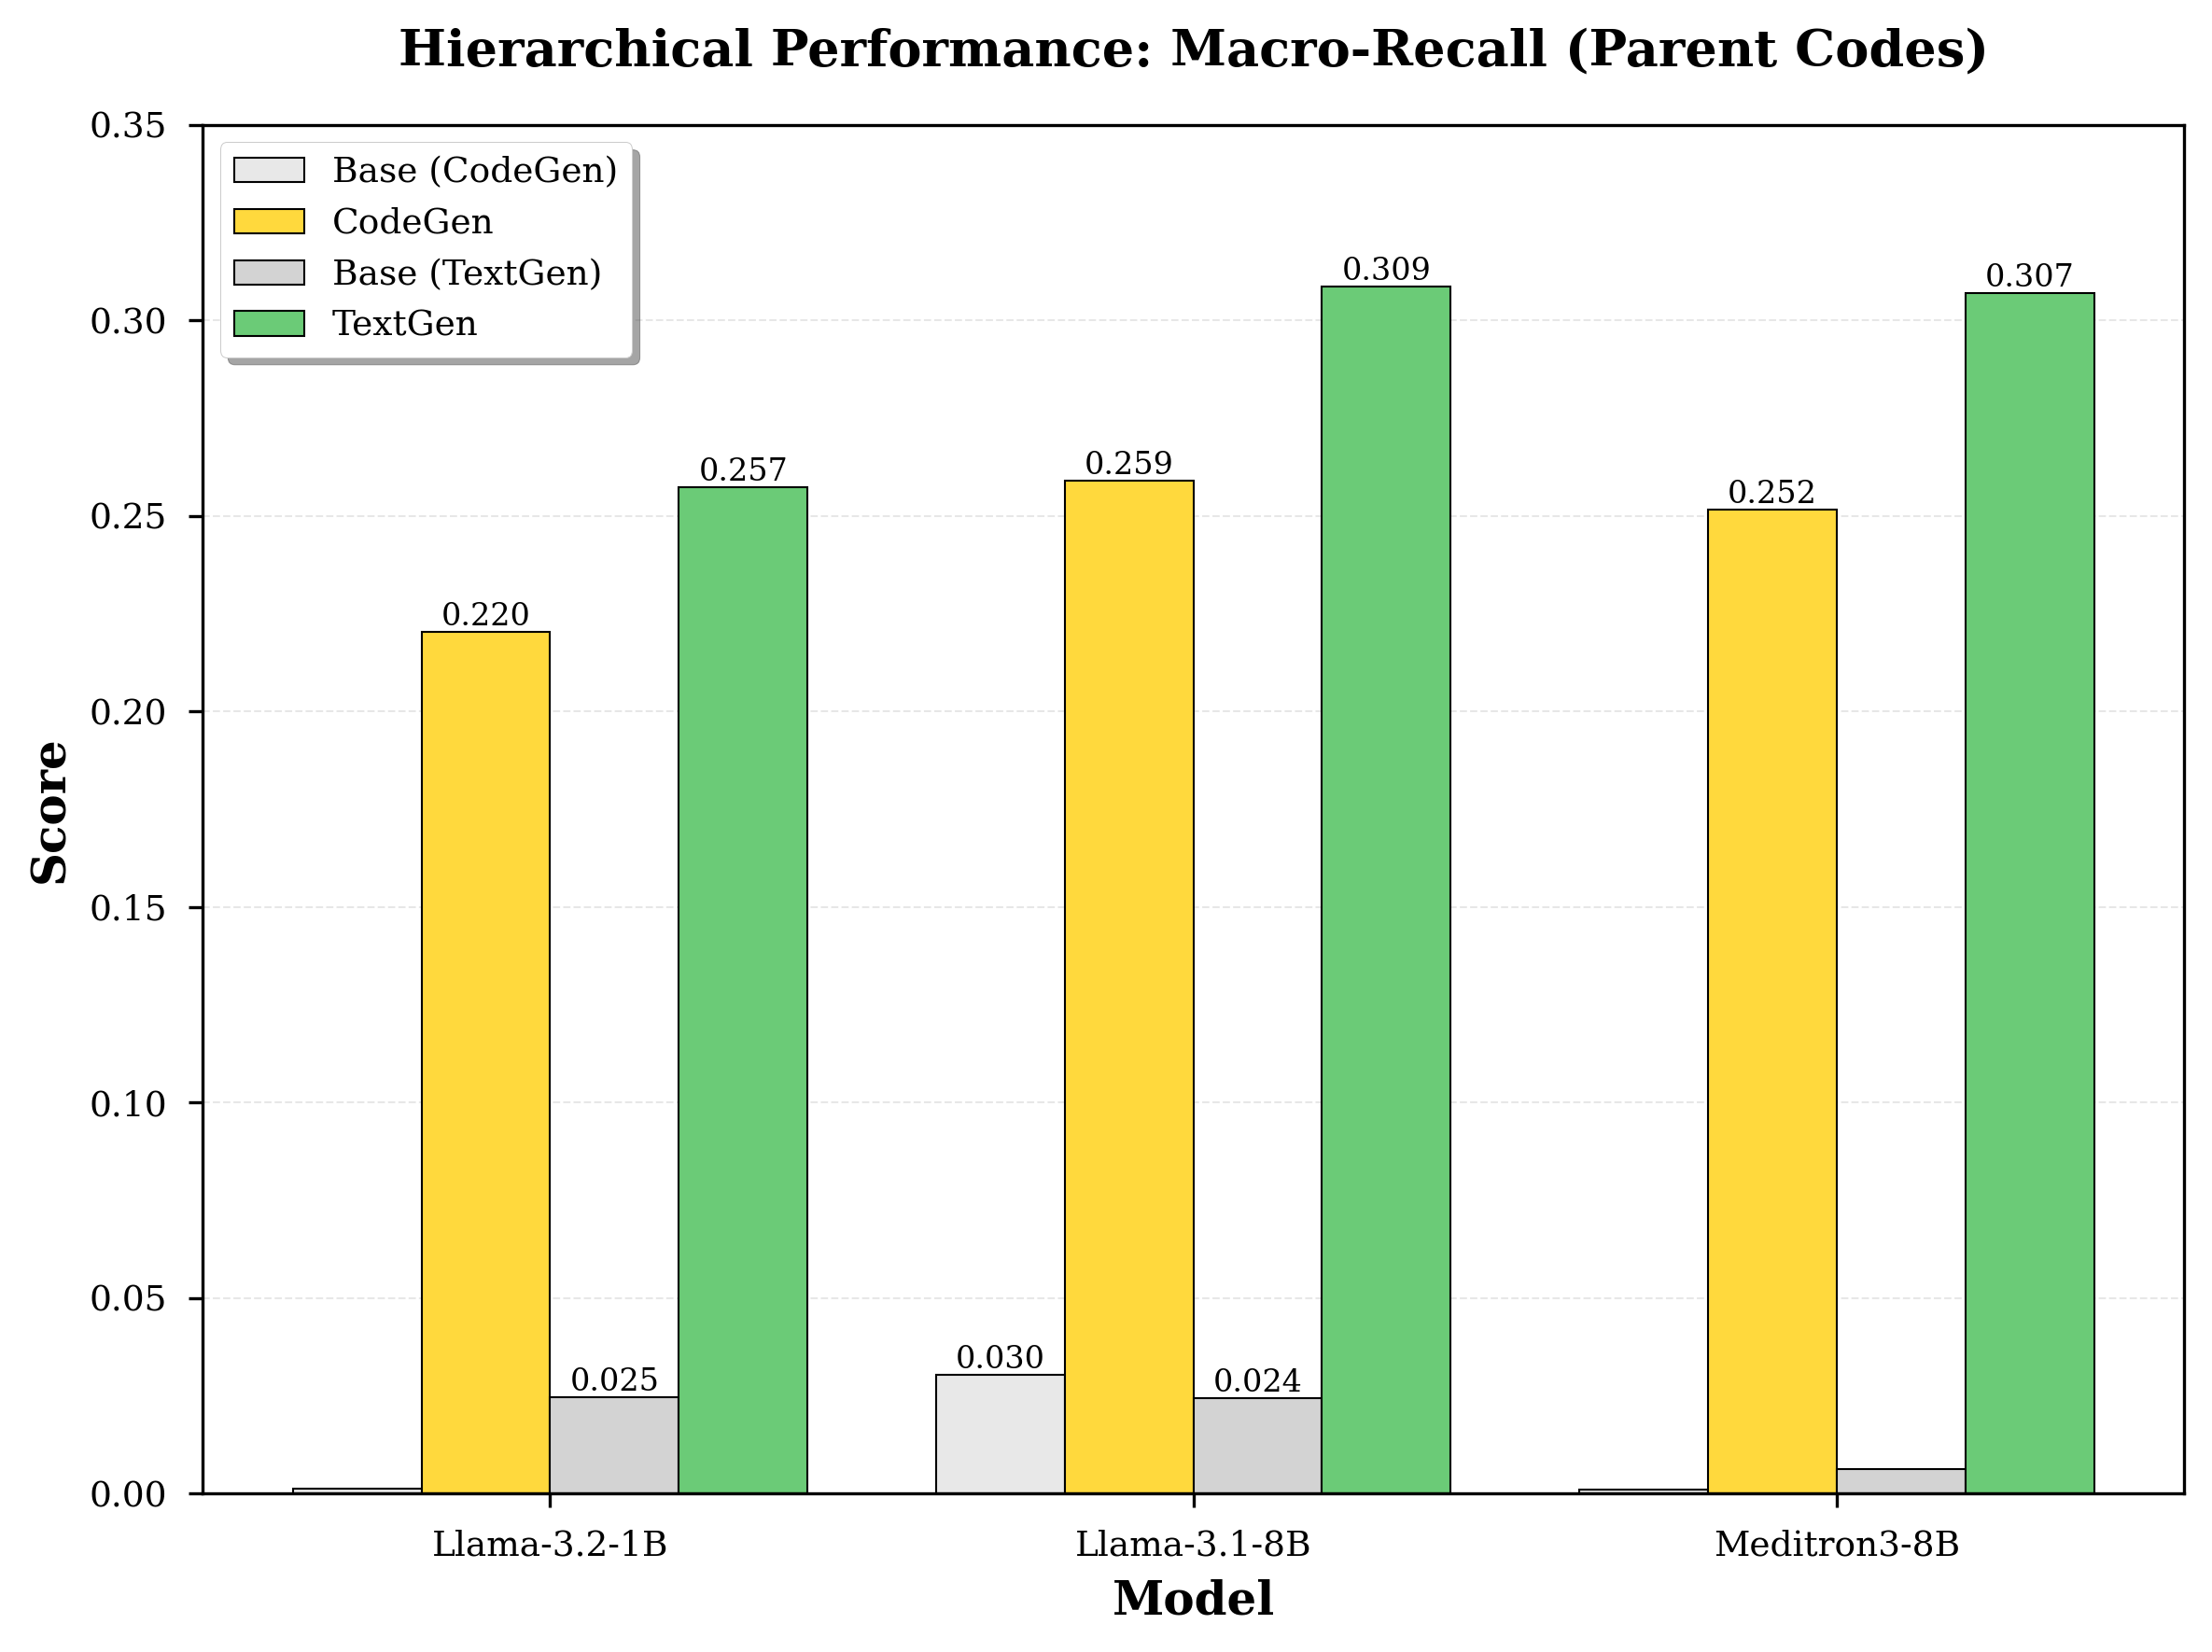
\includegraphics[width=\linewidth]{Images/Plots_thesis/parent_macro_recall.png}
%         \caption{Parent macro-Recall}
%         \label{fig:task1-parent-macroR}
%     \end{subfigure}\hfill
%     \begin{subfigure}{0.32\textwidth}
%         \centering
%         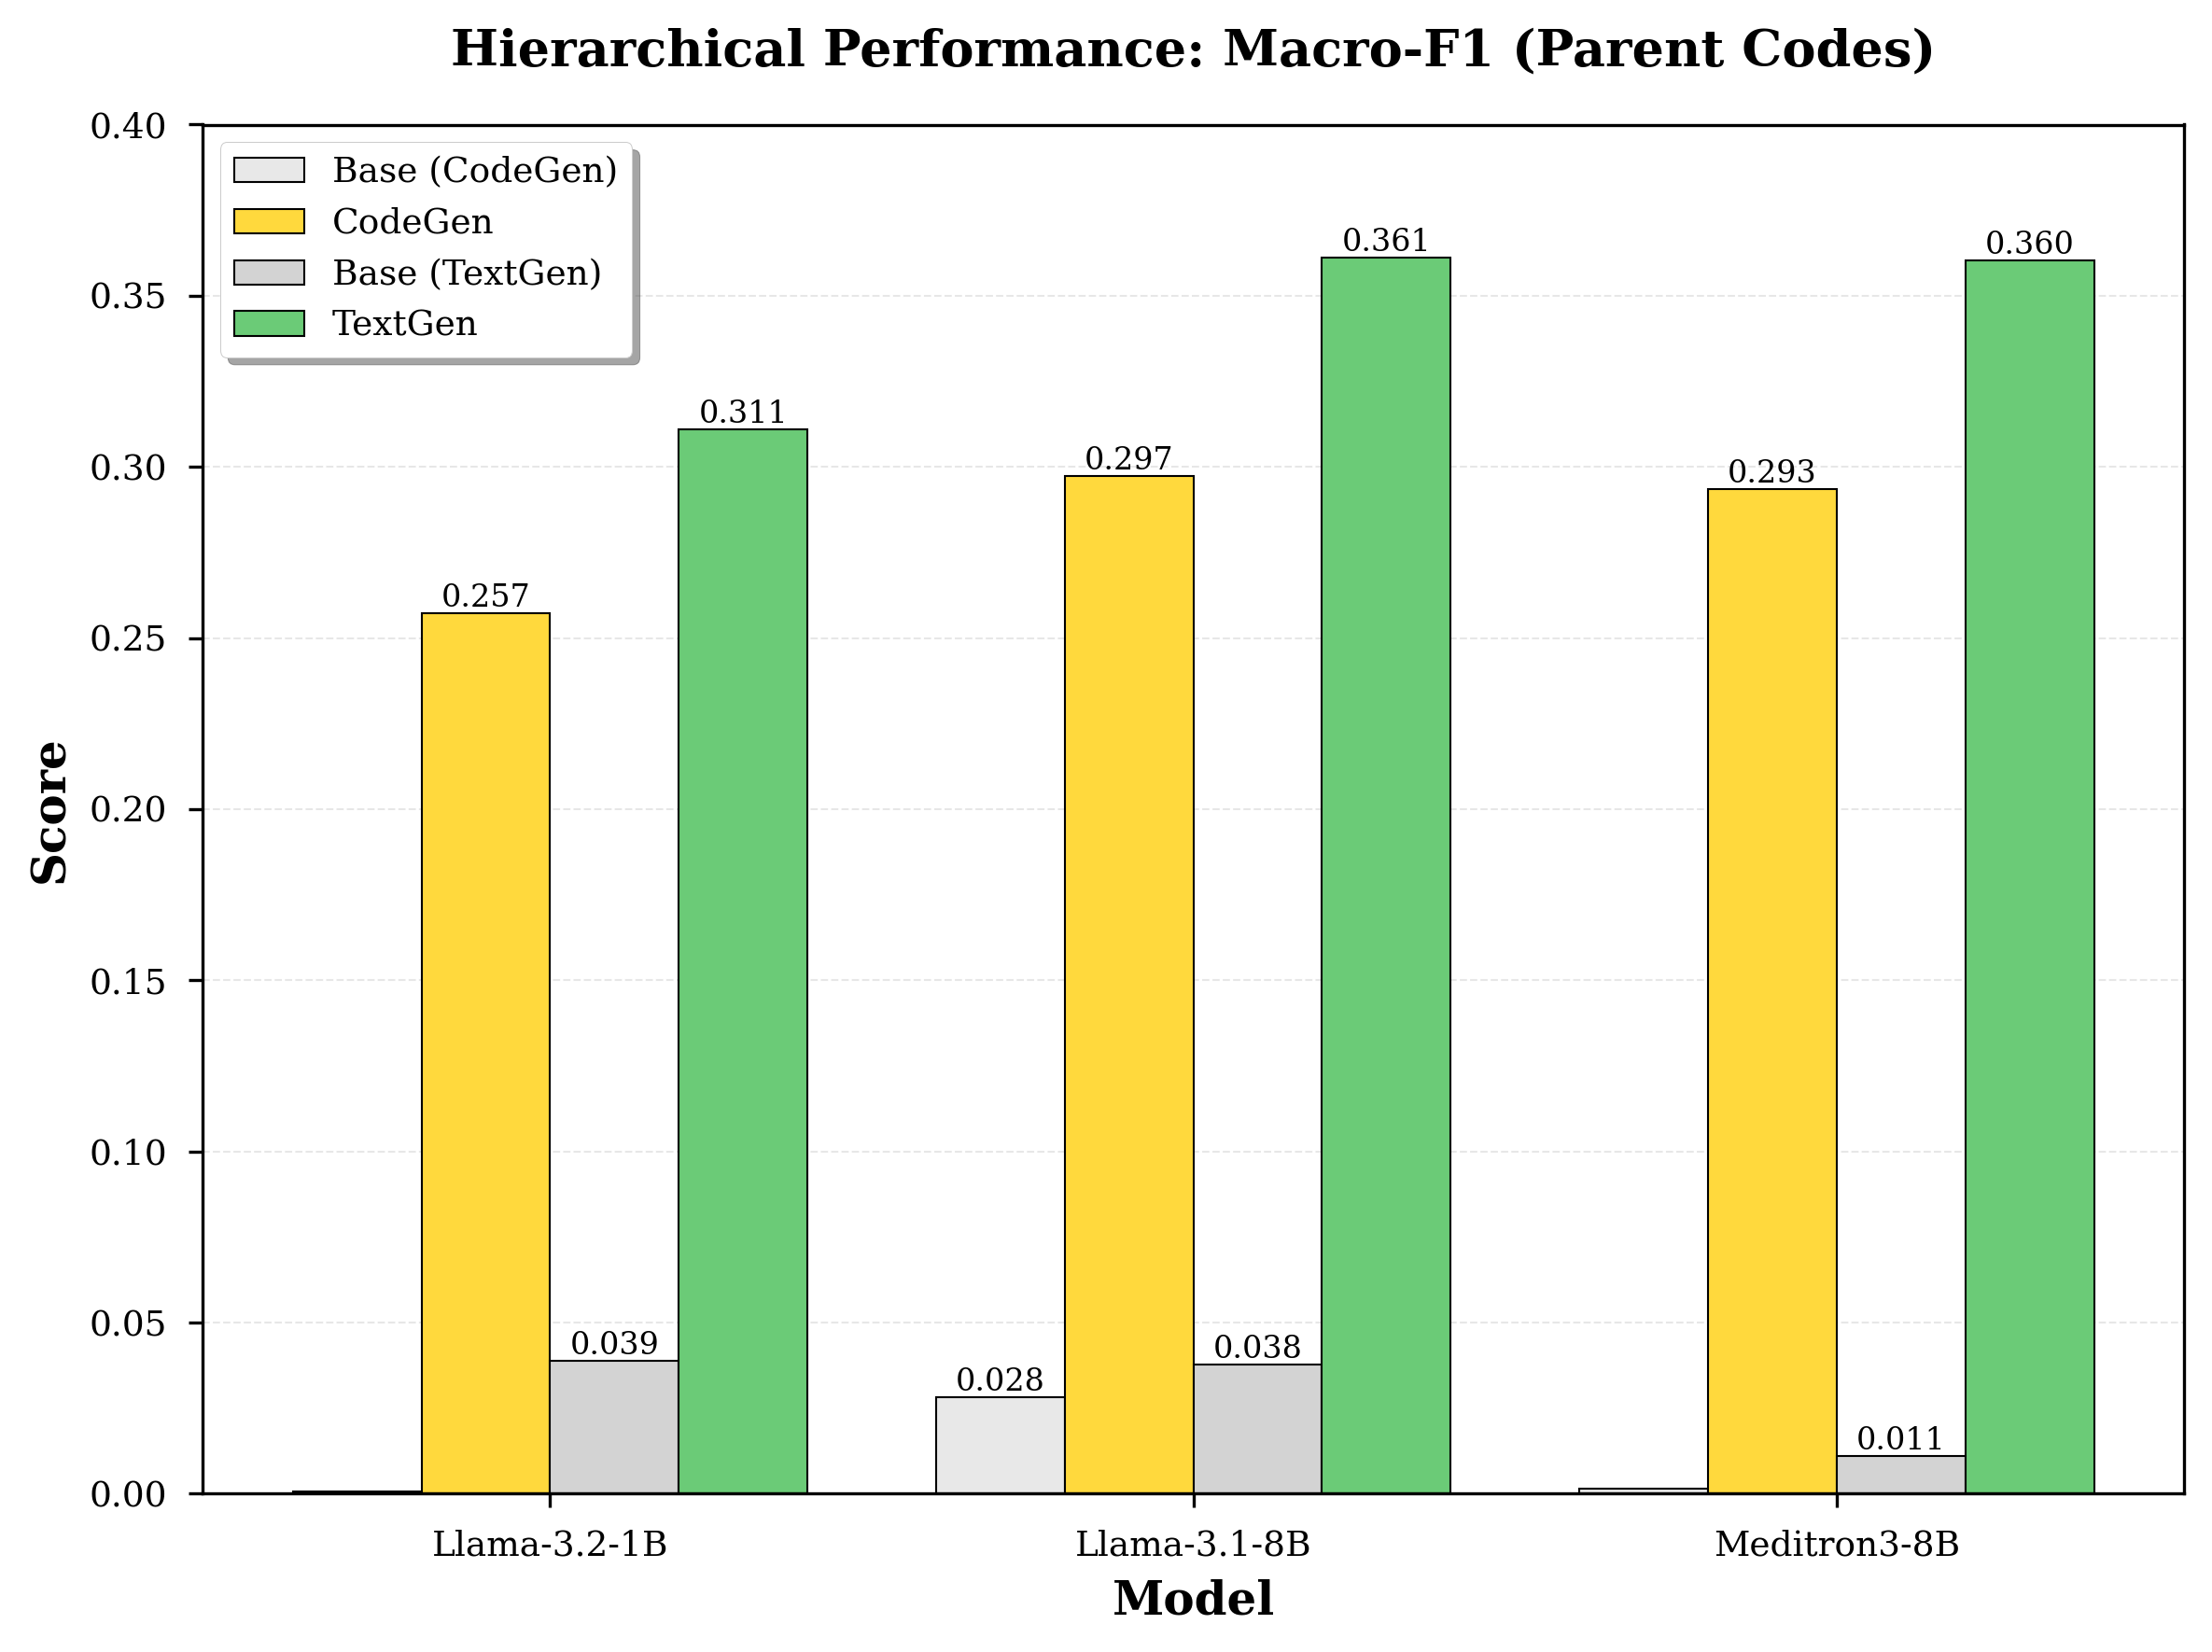
\includegraphics[width=\linewidth]{Images/Plots_thesis/parent_macro_f1.png}
%         \caption{Parent macro-F1}
%         \label{fig:task1-parent-macroF1}
%     \end{subfigure}

%     \caption{Task~1 hierarchical evaluation: parent-level micro/macro precision, recall, and F1 for \textbf{Base}, \textbf{CodeGen}, and \textbf{TextGen} across backbones. Parent evaluation reveals clinically meaningful ``near misses'' at the full-code level.}
%     \label{fig:task1-parent-metrics}
% \end{figure}

% % ============================================================
% \subsection{Head--Tail Behaviour: Performance on Frequent vs.\ Rare Codes}
% \label{subsec:results-task1-headtail}

% Overall micro-averaged metrics are dominated by frequent codes, while macro-averaged metrics are sensitive to poor tail performance. To explicitly characterise label imbalance, we evaluate models on two extremal subsets of the label space: the \textbf{Top-50} (Head-50) and \textbf{Bottom-50} (Tail-50) ICD-9 codes, defined by global code frequency across all splits (Section~\ref{subsec:head-tail-cohort}). 

% \paragraph{Top-50 codes (Head-50).}
% Table~\ref{tab:task1-top50} shows that TextGen achieves strong performance on frequent diagnoses across all backbones and substantially exceeds CodeGen. This indicates that when sufficient supervised signal exists, TextGen can use its limited output budget effectively to prioritise prevalent diagnoses.

% \begin{table}[t]
% \centering
% \caption{Task~1 performance restricted to the Top-50 most frequent ICD-9 codes (Head-50) on the test set.}
% \label{tab:task1-top50}
% \begin{tabular}{llcc}
% \toprule
% \textbf{Backbone} & \textbf{Method} & \textbf{Micro-F1} & \textbf{Macro-F1} \\
% \midrule
% \multirow{4}{*}{Llama-3.2-1B}
% & Base (CodeGen) & 0.0002 & 0.0001 \\
% & CodeGen        & 0.3292 & 0.2670 \\
% & Base (TextGen) & 0.0496 & 0.0351 \\
% & TextGen        & \textbf{0.5329} & \textbf{0.4846} \\
% \midrule
% \multirow{4}{*}{Llama-3.1-8B}
% & Base (CodeGen) & 0.0646 & 0.0315 \\
% & CodeGen        & 0.3413 & 0.2784 \\
% & Base (TextGen) & 0.0439 & 0.0300 \\
% & TextGen        & \textbf{0.5876} & \textbf{0.5347} \\
% \midrule
% \multirow{4}{*}{Meditron-8B}
% & Base (CodeGen) & 0.0101 & 0.0054 \\
% & CodeGen        & 0.3342 & 0.2723 \\
% & Base (TextGen) & 0.0030 & 0.0028 \\
% & TextGen        & \textbf{0.5845} & \textbf{0.5253} \\
% \bottomrule
% \end{tabular}
% \end{table}

% \paragraph{Bottom-50 codes (Tail-50).}
% Table~\ref{tab:task1-bottom50} reveals sharp degradation on rare diagnoses. Tail-50 values can be extremely small because each rare code has low support in the test set; even a small number of additional correct predictions can change tail micro/macro metrics substantially. Nevertheless, the consistent head--tail gap confirms that rare-code recovery is a core bottleneck under both data sparsity and a strict 12-output constraint, motivating knowledge augmentation as a targeted mechanism to improve tail coverage.

% \begin{table}[t]
% \centering
% \caption{Task~1 performance restricted to the Bottom-50 rarest ICD-9 codes (Tail-50) on the test set.}
% \label{tab:task1-bottom50}
% \begin{tabular}{llcc}
% \toprule
% \textbf{Backbone} & \textbf{Method} & \textbf{Micro-F1} & \textbf{Macro-F1} \\
% \midrule
% \multirow{4}{*}{Llama-3.2-1B}
% & Base (CodeGen) & 0.0000 & 0.0000 \\
% & CodeGen        & 0.1304 & 0.0367 \\
% & Base (TextGen) & 0.0000 & 0.0000 \\
% & TextGen        & \textbf{0.1429} & \textbf{0.0655} \\
% \midrule
% \multirow{4}{*}{Llama-3.1-8B}
% & Base (CodeGen) & 0.0129 & 0.0025 \\
% & CodeGen        & 0.1200 & 0.0600 \\
% & Base (TextGen) & 0.0488 & 0.0345 \\
% & TextGen        & \textbf{0.1250} & \textbf{0.0713} \\
% \midrule
% \multirow{4}{*}{Meditron-8B}
% & Base (CodeGen) & 0.0000 & 0.0000 \\
% & CodeGen        & 0.1304 & 0.0133 \\
% & Base (TextGen) & 0.0000 & 0.0000 \\
% & TextGen        & \textbf{0.1518} & \textbf{0.0747} \\
% \bottomrule
% \end{tabular}
% \end{table}

% \begin{figure}[t]
%     \centering
%     % first row
%     \begin{subfigure}{0.48\textwidth}
%         \centering
%         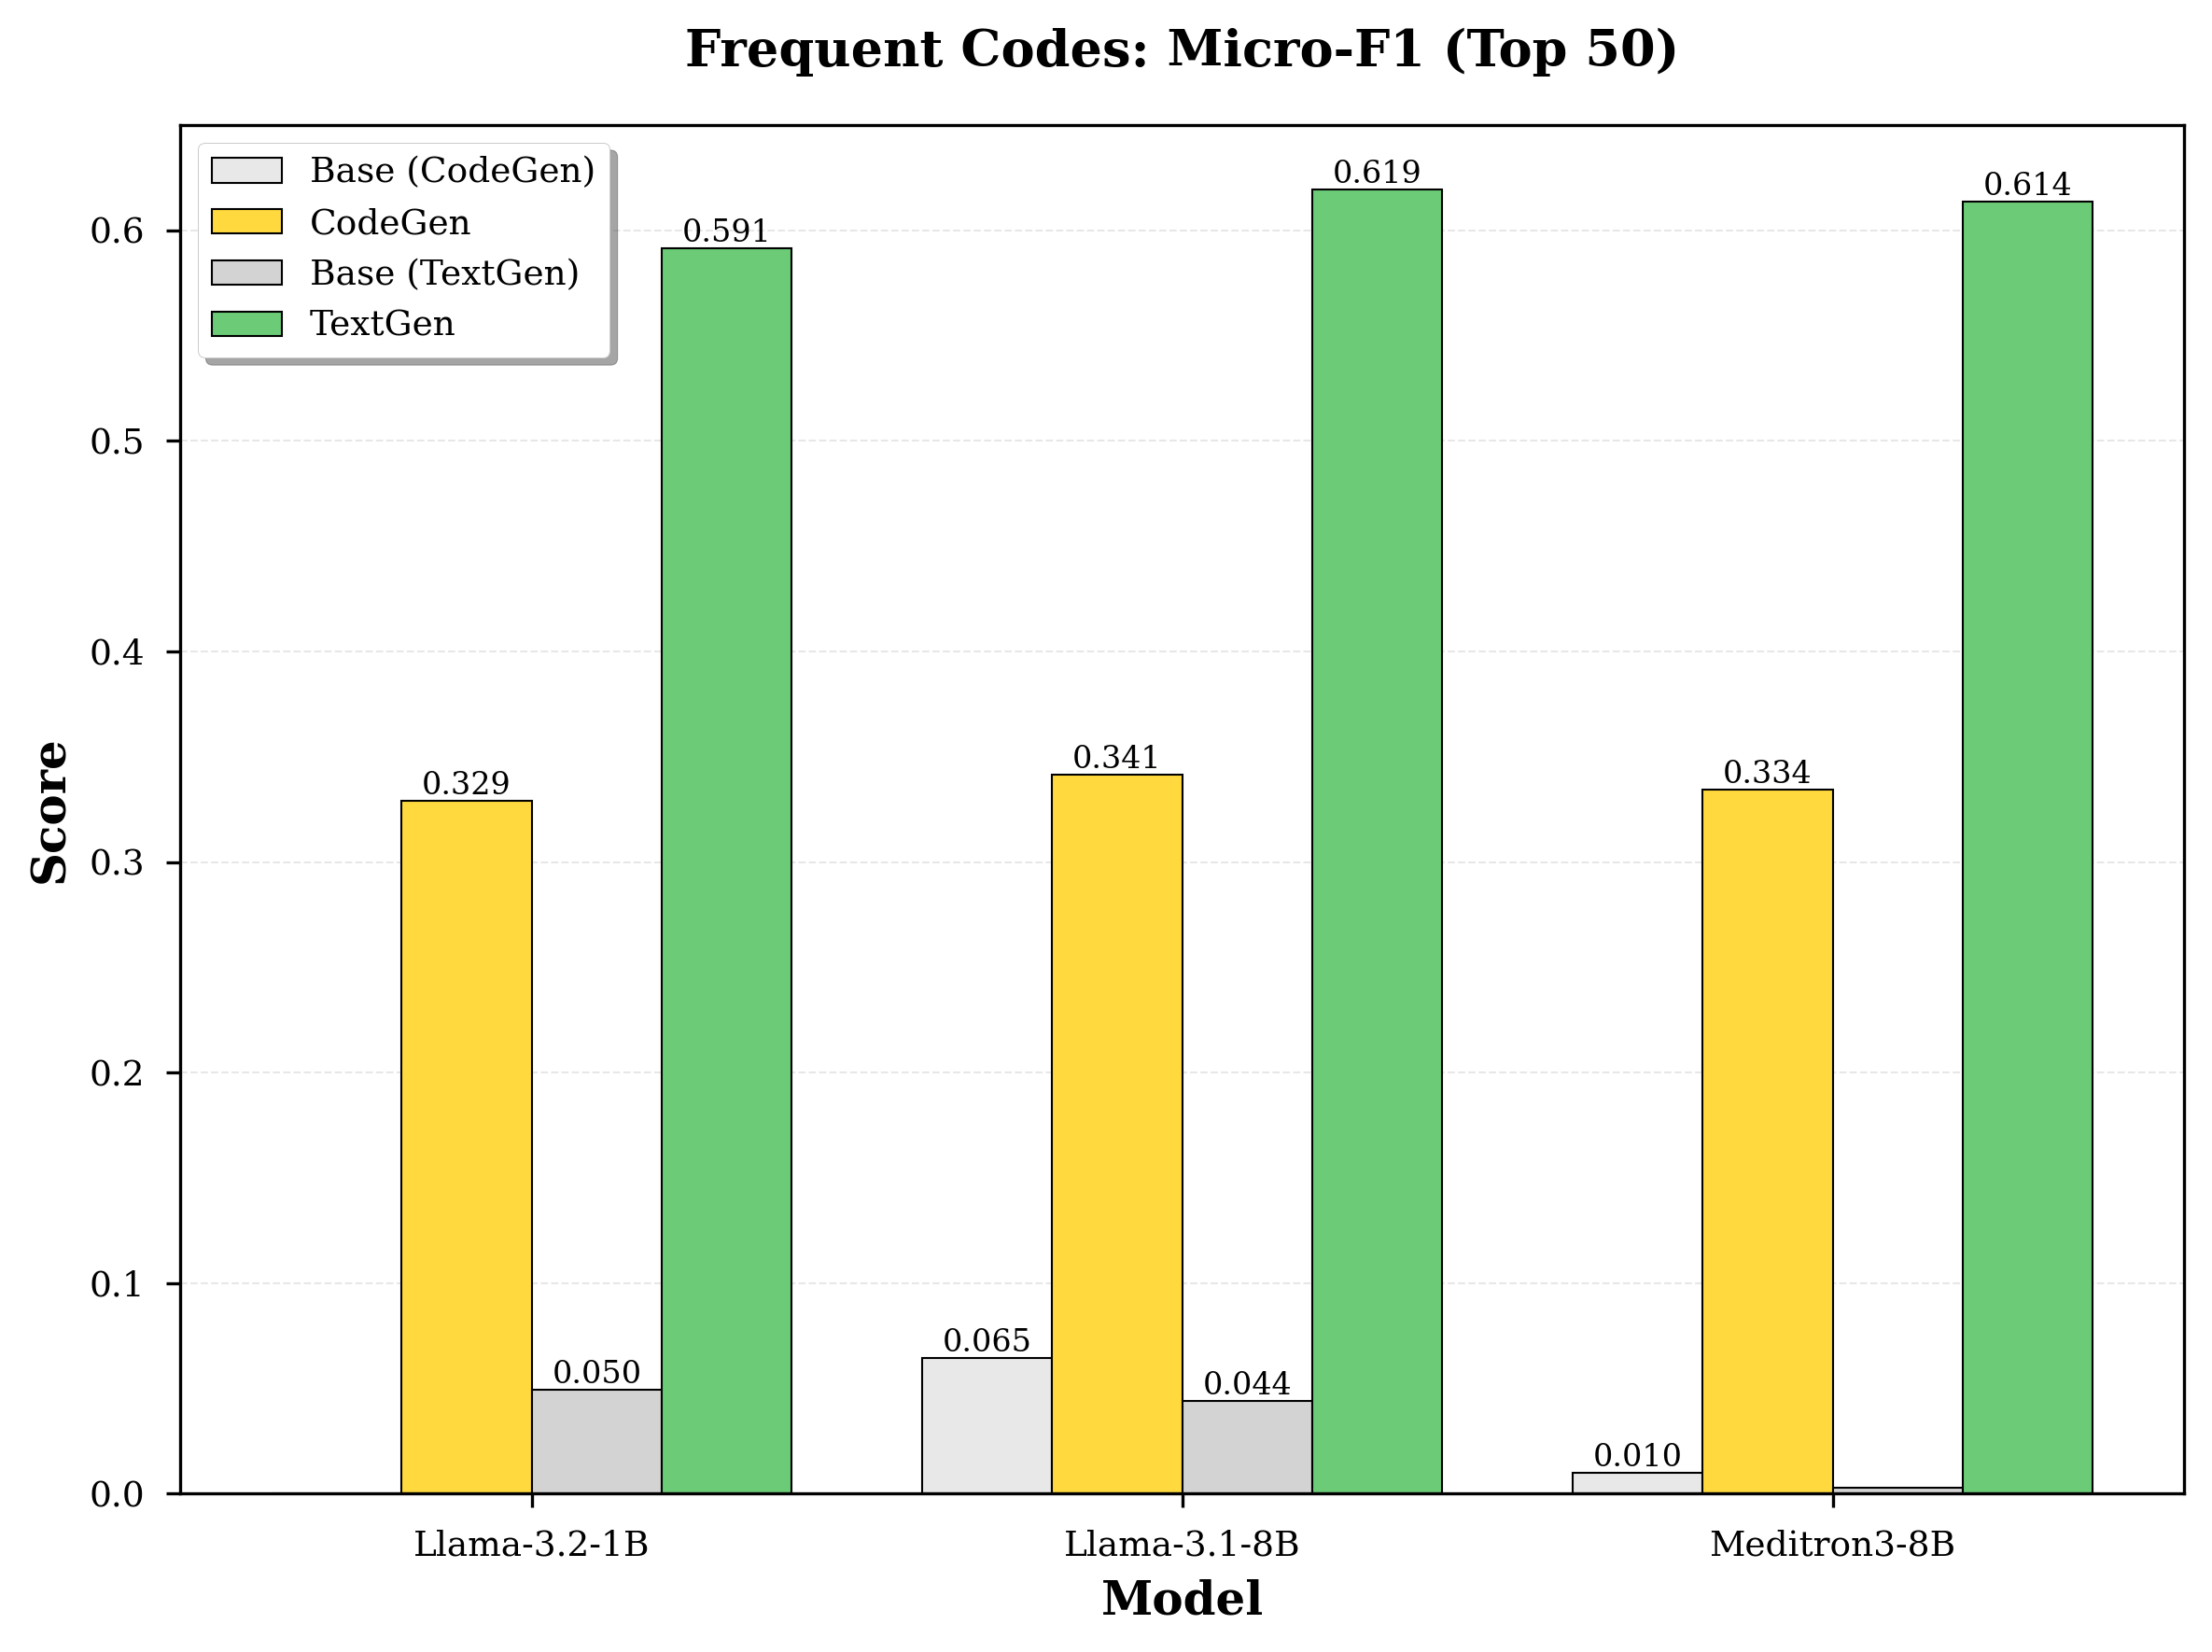
\includegraphics[width=\linewidth]{Images/Plots_thesis/top50_micro_f1.png}
%         \caption{Top-50 micro-F1}
%         \label{fig:task1-top50-microF1}
%     \end{subfigure}\hfill
%     \begin{subfigure}{0.48\textwidth}
%         \centering
%         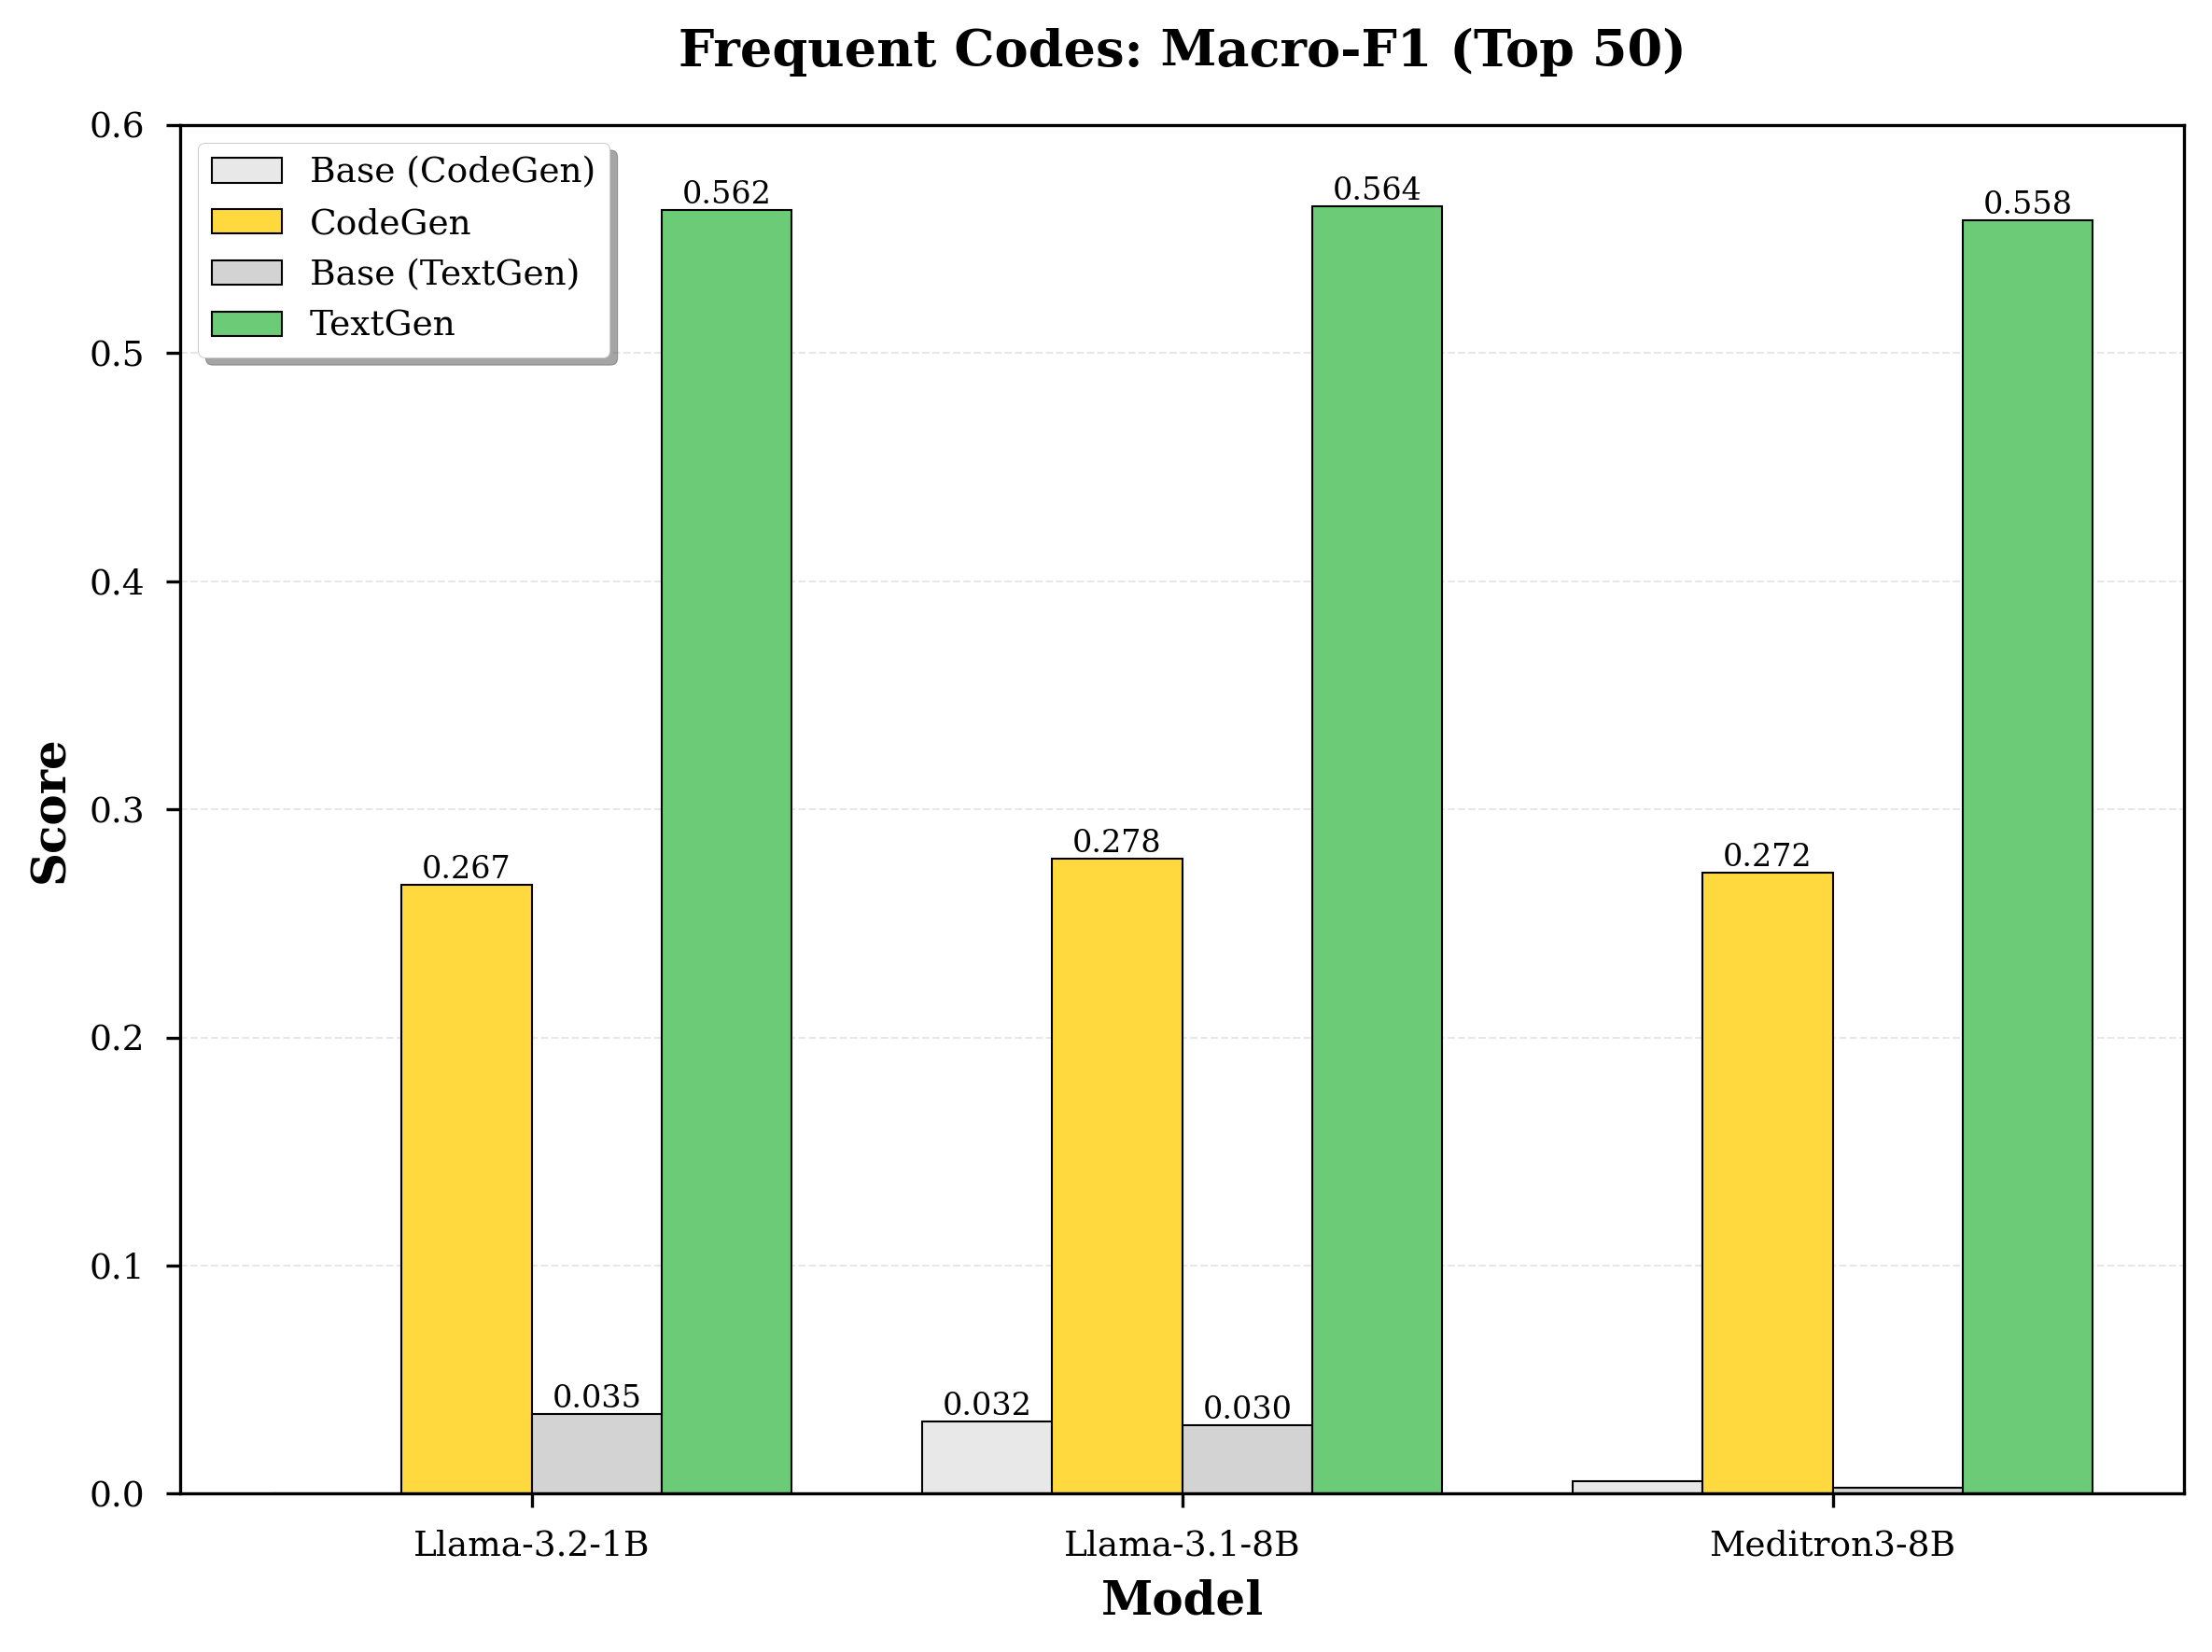
\includegraphics[width=\linewidth]{Images/Plots_thesis/top50_macro_f1.png}
%         \caption{Top-50 macro-F1}
%         \label{fig:task1-top50-macroF1}
%     \end{subfigure}

%     \vspace{0.3cm}

%     % second row
%     \begin{subfigure}{0.48\textwidth}
%         \centering
%         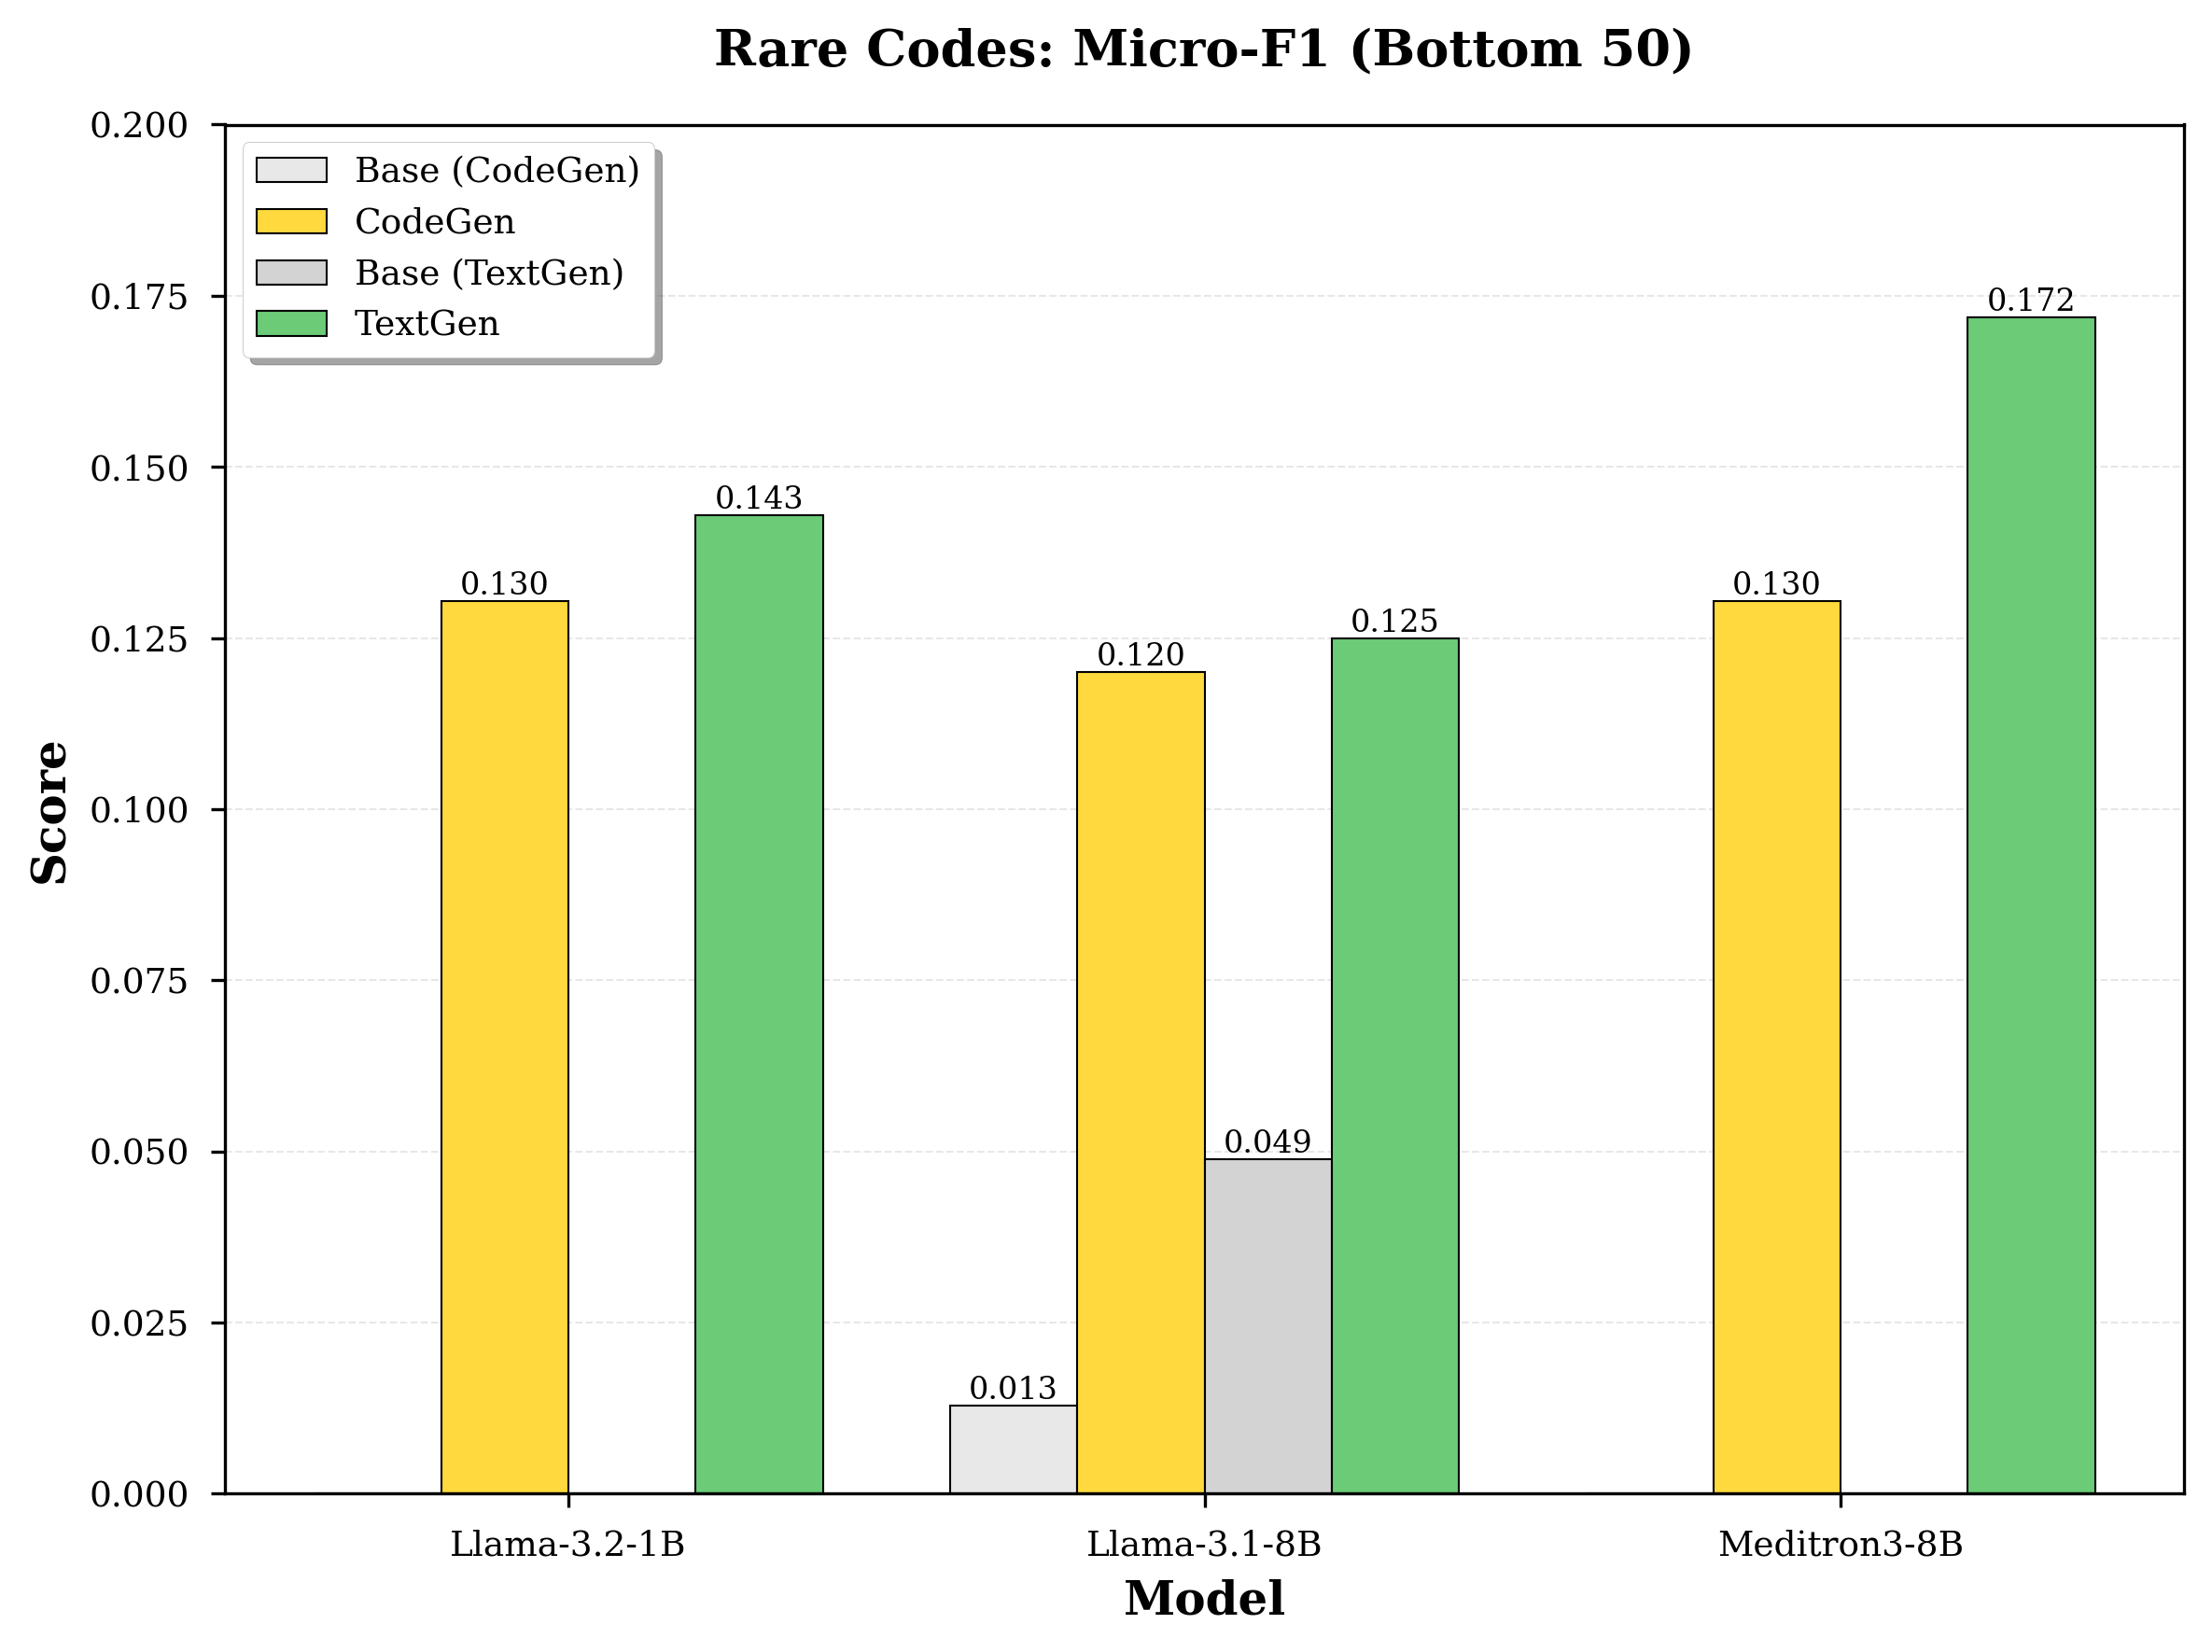
\includegraphics[width=\linewidth]{Images/Plots_thesis/bottom50_micro_f1.png}
%         \caption{Bottom-50 micro-F1}
%         \label{fig:task1-bottom50-microF1}
%     \end{subfigure}\hfill
%     \begin{subfigure}{0.48\textwidth}
%         \centering
%         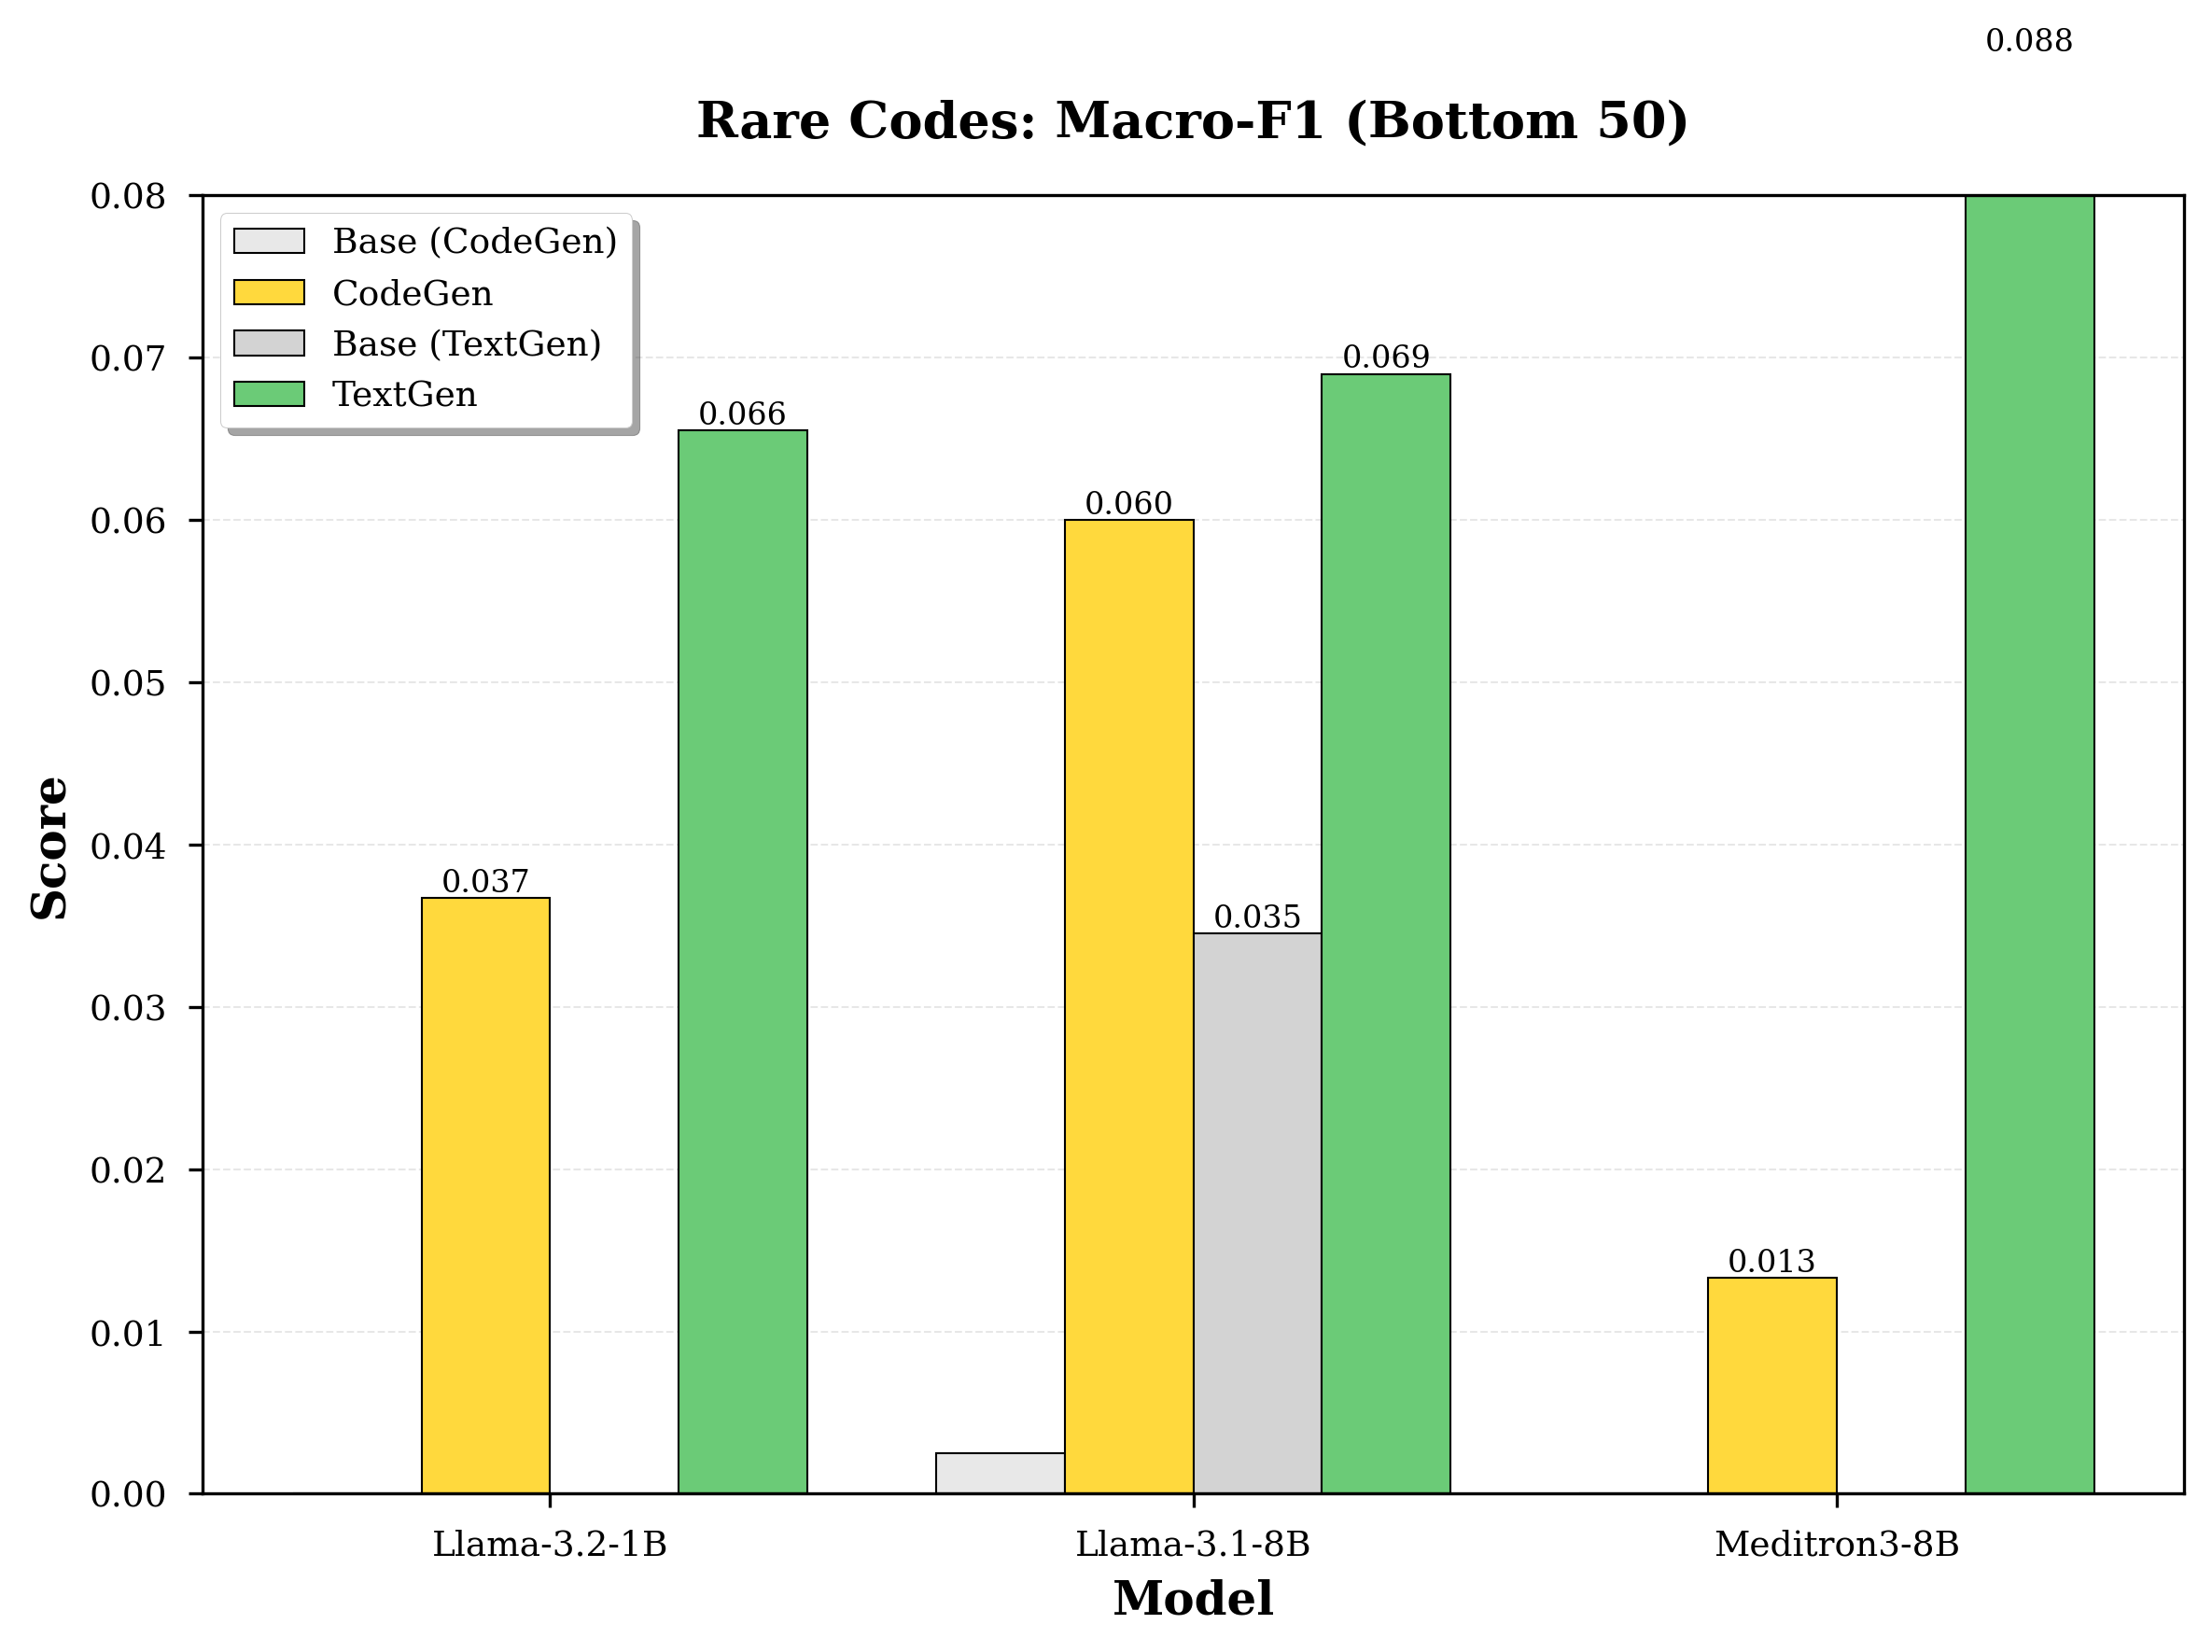
\includegraphics[width=\linewidth]{Images/Plots_thesis/bottom50_macro_f1.png}
%         \caption{Bottom-50 macro-F1}
%         \label{fig:task1-bottom50-macroF1}
%     \end{subfigure}

%     \caption{Task~1: Head-50 vs Tail-50 comparison (e.g., micro-F1 and macro-F1) across CodeGen vs TextGen and base model}
%     \label{fig:task1-headtail-metrics}
% \end{figure}                                   

% % ============================================================
% \subsection{Ablation: Augmenting KG Paths at Inference Only (No KG Training)}
% \label{subsec:results-task1-kg-inference-only}

% We next test whether structured knowledge helps \emph{without changing training}. Concretely, we take a strong fine-tuned TextGen baseline and \textbf{only modify inference} by injecting retrieved KG paths into the prompt. This is an ablation of \emph{prompt-time grounding}: the model sees KG context at test time, but it has never been trained to consume or rely on the KG section.

% We report results for two retrieval scopes: \textbf{H1} and \textbf{H2}. Importantly, the baseline used for this ablation is evaluated with \textbf{no KG paths at inference}, providing a clean reference point for ``KG at inference-only''.

% \paragraph{Overall code-level effect.}
% Table~\ref{tab:task1-kg-inference-overall} shows that injecting KG paths \emph{at inference only} does \textbf{not} produce consistent gains in overall performance; in most cases it slightly degrades micro-F1/macro-F1 relative to the baseline without KG at inference.

% \begin{table}[t]
% \centering
% \caption{Task~1 inference-only KG ablation (overall code-level). Same fine-tuned TextGen checkpoint; only inference prompt differs.}
% \label{tab:task1-kg-inference-overall}
% \begin{tabular}{lcccccc}
% \toprule
% \textbf{Model} &
% \multicolumn{2}{c}{\textbf{Baseline (no KG @ inf)}} &
% \multicolumn{2}{c}{\textbf{+ KG H1 @ inf}} &
% \multicolumn{2}{c}{\textbf{+ KG H2 @ inf}} \\
% \cmidrule(lr){2-3}\cmidrule(lr){4-5}\cmidrule(lr){6-7}
% & \textbf{Micro-F1} & \textbf{Macro-F1}
% & \textbf{Micro-F1} & \textbf{Macro-F1}
% & \textbf{Micro-F1} & \textbf{Macro-F1} \\
% \midrule
% Llama-3.2-1B   & 0.4313 & 0.2065 & 0.3764 & 0.1807 & 0.4056 & 0.1904 \\
% Llama-3.1-8B   & 0.4585 & 0.2457 & 0.4441 & 0.2370 & 0.4510 & 0.2450 \\
% Meditron3-8B   & 0.4556 & 0.2457 & 0.4440 & 0.2382 & 0.4527 & 0.2404 \\
% \bottomrule
% \end{tabular}
% \end{table}

% \paragraph{Head vs.\ tail behaviour.}
% Inference-only KG prompting also fails to reliably close the head--tail gap. On Head-50, KG injection consistently reduces performance (Table~\ref{tab:task1-kg-inference-top50}). On Tail-50, effects are unstable: in some settings (e.g., \texttt{Llama-3.1-8B} with H2) the tail micro-F1 increases, but this does not translate into consistent overall gains (Table~\ref{tab:task1-kg-inference-bottom50}).

% \begin{table}[t]
% \centering
% \caption{Inference-only KG ablation on Top-50 (Head-50).}
% \label{tab:task1-kg-inference-top50}
% \begin{tabular}{lcccccc}
% \toprule
% \textbf{Model} &
% \multicolumn{2}{c}{\textbf{Baseline}} &
% \multicolumn{2}{c}{\textbf{+ KG H1}} &
% \multicolumn{2}{c}{\textbf{+ KG H2}} \\
% \cmidrule(lr){2-3}\cmidrule(lr){4-5}\cmidrule(lr){6-7}
% & \textbf{Micro-F1} & \textbf{Macro-F1}
% & \textbf{Micro-F1} & \textbf{Macro-F1}
% & \textbf{Micro-F1} & \textbf{Macro-F1} \\
% \midrule
% Llama-3.2-1B   & 0.5914 & 0.5625 & 0.5329 & 0.4846 & 0.5733 & 0.52 \\
% Llama-3.1-8B   & 0.6193 & 0.5644 & 0.5876 & 0.5347 & 0.6102 & 0.5566 \\
% Meditron3-8B   & 0.6136 & 0.5583 & 0.5583 & 0.5253 & 0.6092 & 0.5524 \\
% \bottomrule
% \end{tabular}
% \end{table}

% \begin{table}[t]
% \centering
% \caption{Inference-only KG ablation on Bottom-50 (Tail-50).}
% \label{tab:task1-kg-inference-bottom50}
% \begin{tabular}{lcccccc}
% \toprule
% \textbf{Model} &
% \multicolumn{2}{c}{\textbf{Baseline}} &
% \multicolumn{2}{c}{\textbf{+ KG H1}} &
% \multicolumn{2}{c}{\textbf{+ KG H2}} \\
% \cmidrule(lr){2-3}\cmidrule(lr){4-5}\cmidrule(lr){6-7}
% & \textbf{Micro-F1} & \textbf{Macro-F1}
% & \textbf{Micro-F1} & \textbf{Macro-F1}
% & \textbf{Micro-F1} & \textbf{Macro-F1} \\
% \midrule
% Llama-3.2-1B   & 0.1429 & 0.0655 & 0.0000 & 0.0000 & 0.0286 & 0.0133 \\
% Llama-3.1-8B   & 0.1250 & 0.0713 & 0.1200 & 0.0713 & 0.1600 & 0.0885 \\
% Meditron3-8B   & 0.1518 & 0.0885 & 0.1429 & 0.0747 & 0.1364 & 0.0747 \\
% \bottomrule
% \end{tabular}
% \end{table}

% \paragraph{Why inference-only KG can fail.}
% A plausible explanation is that na\"ively injecting KG paths introduces a \textbf{distribution shift} in the prompt: the model is not trained to treat KG paths as privileged evidence, and may (i) attend to irrelevant or noisy relations, (ii) allocate its limited 12-output budget to KG-correlated but incorrect hypotheses, or (iii) suffer from context dilution when long retrieval text competes with clinically salient spans from the note. This motivates the next step: \emph{train the model to use KG context}.

% \begin{figure}[t]
%     \centering
%     
\includegraphics[width=0.92\textwidth]{Images/Empty.png}
%     \caption{(Placeholder) Inference-only KG ablation: grouped bars comparing Baseline (no KG @ inf) vs +KG(H1/H2) @ inf across overall/parent/head/tail micro-F1.}
%     \label{fig:task1-kg-inference-plots}
% \end{figure}

% % ============================================================
% \subsection{KG-Augmented Fine-Tuning (RAG-Style Variants)}
% \label{subsec:results-task1-kg-rag}

% Motivated by the weak and inconsistent behaviour of inference-only KG prompting, we move to \textbf{KG-augmented fine-tuning}: during training, prompts are enriched with retrieved KG paths so the model learns to condition on structured relations. At inference, the same retrieval mechanism is applied, yielding a RAG-style pipeline.

% We evaluate two retrieval scopes (\textbf{H1} vs.\ \textbf{H2}) and two integration strategies (\textbf{Unweighted} vs.\ \textbf{Weighted}). The baseline for these comparisons is the fine-tuned TextGen model evaluated \textbf{without KG paths at inference} (as in Section~\ref{subsec:results-task1-kg-inference-only}). This makes the comparison strict: KG/RAG must outperform a strong baseline that is not exposed to potentially noisy KG text at test time.

% \paragraph{Overall code-level performance.}
% Table~\ref{tab:task1-rag-overall} shows that KG-augmented fine-tuning yields \textbf{consistent improvements} in micro-F1 and macro-F1 over the baseline across all backbones. Weighted variants are strongest overall, suggesting that relevance-controlled KG selection helps reduce noise and stabilise gains.

% \begin{table}[t]
% \centering
% \caption{Task~1 overall code-level metrics for KG-augmented (RAG) variants vs.\ Baseline TextGen (no KG at inference). Test set evaluation.}
% \label{tab:task1-rag-overall}
% \resizebox{\textwidth}{!}{
% \begin{tabular}{llcccccc}
% \toprule
% \textbf{Model} & \textbf{Method} & \textbf{Micro-F1} & \textbf{Macro-F1} & \textbf{Micro-P} & \textbf{Macro-P} & \textbf{Micro-R} & \textbf{Macro-R} \\
% \midrule
% Llama-3.2-1B & H1 Unweighted & 0.4452 & 0.2134 & 0.5190 & 0.2862 & 0.3891 & 0.1941 \\
% Llama-3.2-1B & H1 Weighted   & \textbf{0.4749} & \textbf{0.2368} & 0.5419 & 0.3068 & 0.4230 & 0.2289 \\
% Llama-3.2-1B & H2 Unweighted & 0.4407 & 0.2143 & 0.5156 & 0.2888 & 0.3842 & 0.1940 \\
% Llama-3.2-1B & H2 Weighted   & 0.4726 & 0.2333 & 0.5462 & 0.3067 & 0.4168 & 0.2234 \\
% Llama-3.2-1B & Baseline TextGen (no KG @ inf) & 0.4313 & 0.2065 & 0.5084 & 0.2540 & 0.3745 & 0.1740 \\
% \midrule
% Llama-3.1-8B & H1 Unweighted & 0.4732 & 0.2546 & 0.5464 & 0.3349 & 0.4168 & 0.2406 \\
% Llama-3.1-8B & H1 Weighted   & \textbf{0.5029} & \textbf{0.2762} & 0.5770 & 0.3565 & 0.4459 & 0.2615 \\
% Llama-3.1-8B & H2 Unweighted & 0.4699 & 0.2558 & 0.5426 & 0.3334 & 0.4139 & 0.2426 \\
% Llama-3.1-8B & H2 Weighted   & 0.4998 & 0.2724 & 0.5739 & 0.3541 & 0.4429 & 0.2581 \\
% Llama-3.1-8B & Baseline TextGen (no KG @ inf) & 0.4585 & 0.2457 & 0.5140 & 0.3338 & 0.4142 & 0.2400 \\
% \midrule
% Meditron3-8B & H1 Unweighted & 0.4700 & 0.2593 & 0.5436 & 0.3424 & 0.4135 & 0.2479 \\
% Meditron3-8B & H1 Weighted   & \textbf{0.5036} & \textbf{0.2793} & 0.5765 & 0.3628 & 0.4473 & 0.2662 \\
% Meditron3-8B & H2 Unweighted & 0.4736 & 0.2563 & 0.5499 & 0.3354 & 0.4153 & 0.2433 \\
% Meditron3-8B & H2 Weighted   & 0.5023 & 0.2750 & 0.5792 & 0.3519 & 0.4437 & 0.2619 \\
% Meditron3-8B & Baseline TextGen (no KG @ inf) & 0.4556 & 0.2457 & 0.5119 & 0.3295 & 0.4135 & 0.2395 \\
% \bottomrule
% \end{tabular}}
% \end{table}

% \begin{figure}[t]
%     \centering
%     
\includegraphics[width=0.92\textwidth]{Images/Empty.png}
%     \caption{(Placeholder) KG/RAG overall metrics: grouped bars (micro/macro P/R/F1) comparing Baseline vs.\ H1/H2 Unweighted vs.\ H1/H2 Weighted per backbone.}
%     \label{fig:task1-rag-overall-plots}
% \end{figure}

% \paragraph{Hierarchical (parent-level) performance.}
% Parent-level metrics also improve with KG-augmented fine-tuning, indicating that gains reflect better diagnostic-family alignment rather than superficial formatting.

% \begin{table}[t]
% \centering
% \caption{Task~1 parent-level hierarchical metrics for KG-augmented (RAG) variants vs.\ Baseline TextGen (no KG at inference). Test set evaluation.}
% \label{tab:task1-rag-parent}
% \resizebox{\textwidth}{!}{
% \begin{tabular}{llcccccc}
% \toprule
% \textbf{Model} & \textbf{Method} & \textbf{Micro-F1} & \textbf{Macro-F1} & \textbf{Micro-P} & \textbf{Macro-P} & \textbf{Micro-R} & \textbf{Macro-R} \\
% \midrule
% Llama-3.2-1B & H1 Unweighted & 0.5388 & 0.3174 & 0.6320 & 0.4162 & 0.4688 & 0.2874 \\
% Llama-3.2-1B & H1 Weighted   & \textbf{0.5736} & \textbf{0.3412} & 0.6571 & 0.4351 & 0.5092 & 0.3155 \\
% Llama-3.2-1B & H2 Unweighted & 0.5389 & 0.3174 & 0.6323 & 0.4163 & 0.4688 & 0.2874 \\
% Llama-3.2-1B & H2 Weighted   & 0.5708 & 0.3401 & 0.6574 & 0.4388 & 0.5012 & 0.3110 \\
% Llama-3.2-1B & Baseline TextGen (no KG @ inf) & 0.5396 & 0.3134 & 0.6248 & 0.4023 & 0.4761 & 0.2827 \\
% \midrule
% Llama-3.1-8B & H1 Unweighted & 0.5632 & 0.3617 & 0.6463 & 0.4622 & 0.4985 & 0.3333 \\
% Llama-3.1-8B & H1 Weighted   & \textbf{0.5926} & \textbf{0.3788} & 0.6765 & 0.4757 & 0.5278 & 0.3507 \\
% Llama-3.1-8B & H2 Unweighted & 0.5598 & 0.3663 & 0.6425 & 0.4621 & 0.4955 & 0.3373 \\
% Llama-3.1-8B & H2 Weighted   & 0.5900 & 0.3789 & 0.6742 & 0.4817 & 0.5247 & 0.3505 \\
% Llama-3.1-8B & Baseline TextGen (no KG @ inf) & 0.5545 & 0.3552 & 0.6202 & 0.4716 & 0.5033 & 0.3455 \\
% \midrule
% Meditron3-8B & H1 Unweighted & 0.5591 & 0.3720 & 0.6430 & 0.4691 & 0.4941 & 0.3480 \\
% Meditron3-8B & H1 Weighted   & \textbf{0.5931} & \textbf{0.3902} & 0.6757 & 0.4907 & 0.5288 & 0.3655 \\
% Meditron3-8B & H2 Unweighted & 0.5631 & 0.3622 & 0.6478 & 0.4475 & 0.4975 & 0.3380 \\
% Meditron3-8B & H2 Weighted   & 0.5910 & 0.3835 & 0.6764 & 0.4742 & 0.5249 & 0.3597 \\
% Meditron3-8B & Baseline TextGen (no KG @ inf) & 0.5456 & 0.3509 & 0.6138 & 0.4621 & 0.4939 & 0.3363 \\
% \bottomrule
% \end{tabular}}
% \end{table}

% \begin{figure}[t]
%     \centering
%     
\includegraphics[width=0.92\textwidth]{Images/Empty.png}
%     \caption{(Placeholder) KG/RAG parent-level metrics: grouped bars (micro/macro P/R/F1) comparing Baseline vs.\ KG variants per backbone.}
%     \label{fig:task1-rag-parent-plots}
% \end{figure}

% \paragraph{Head-50 vs.\ Tail-50 effects (long-tail focus).}
% Tables~\ref{tab:task1-rag-top50} and \ref{tab:task1-rag-tail50} decompose KG gains by frequency strata. Head-50 gains are moderate; the key scientific question is whether KG helps the \emph{tail} under sparse supervision and a strict 12-output constraint.

% \begin{table}[t]
% \centering
% \caption{Task~1 Top-50 (Head-50) metrics for KG-augmented variants vs.\ Baseline TextGen (no KG at inference).}
% \label{tab:task1-rag-top50}
% \resizebox{\textwidth}{!}{
% \begin{tabular}{llcccccc}
% \toprule
% \textbf{Model} & \textbf{Method} & \textbf{Micro-F1} & \textbf{Macro-F1} & \textbf{Micro-P} & \textbf{Macro-P} & \textbf{Micro-R} & \textbf{Macro-R} \\
% \midrule
% Llama-3.2-1B & H1 Unweighted & 0.6009 & 0.5473 & 0.6308 & 0.6134 & 0.5729 & 0.5110 \\
% Llama-3.2-1B & H1 Weighted   & \textbf{0.6375} & \textbf{0.5839} & 0.6590 & 0.6391 & 0.6173 & 0.5563 \\
% Llama-3.2-1B & H2 Unweighted & 0.6005 & 0.5474 & 0.6337 & 0.6159 & 0.5700 & 0.5117 \\
% Llama-3.2-1B & H2 Weighted   & 0.6334 & 0.5799 & 0.6637 & 0.6451 & 0.6055 & 0.5451 \\
% Llama-3.2-1B & Baseline TextGen (no KG @ inf) & 0.6011 & 0.5486 & 0.6413 & 0.6528 & 0.5655 & 0.5136 \\
% \midrule
% Llama-3.1-8B & H1 Unweighted & 0.6259 & 0.5683 & 0.6513 & 0.6323 & 0.6017 & 0.5387 \\
% Llama-3.1-8B & H1 Weighted   & \textbf{0.6535} & \textbf{0.5952} & 0.6780 & 0.6608 & 0.6308 & 0.5669 \\
% Llama-3.1-8B & H2 Unweighted & 0.6209 & 0.5635 & 0.6468 & 0.6282 & 0.5974 & 0.5340 \\
% Llama-3.1-8B & H2 Weighted   & 0.6500 & 0.5927 & 0.6720 & 0.6562 & 0.6294 & 0.5652 \\
% Llama-3.1-8B & Baseline TextGen (no KG @ inf) & 0.5984 & 0.5443 & 0.6322 & 0.6280 & 0.5680 & 0.5195 \\
% \midrule
% Meditron3-8B & H1 Unweighted & 0.6162 & 0.5596 & 0.6430 & 0.6231 & 0.5914 & 0.5288 \\
% Meditron3-8B & H1 Weighted   & \textbf{0.6529} & \textbf{0.5954} & 0.6791 & 0.6611 & 0.6288 & 0.5648 \\
% Meditron3-8B & H2 Unweighted & 0.6238 & 0.5673 & 0.6523 & 0.6339 & 0.5976 & 0.5352 \\
% Meditron3-8B & H2 Weighted   & 0.6529 & 0.5946 & 0.6826 & 0.6624 & 0.6257 & 0.5636 \\
% Meditron3-8B & Baseline TextGen (no KG @ inf) & 0.5879 & 0.5276 & 0.6298 & 0.6310 & 0.5514 & 0.4977 \\
% \bottomrule
% \end{tabular}}
% \end{table}

% \begin{table}[t]
% \centering
% \caption{Task~1 Bottom-50 (Tail-50) metrics for KG-augmented variants vs.\ Baseline TextGen (no KG at inference).}
% \label{tab:task1-rag-tail50}
% \resizebox{\textwidth}{!}{
% \begin{tabular}{llcccccc}
% \toprule
% \textbf{Model} & \textbf{Method} & \textbf{Micro-F1} & \textbf{Macro-F1} & \textbf{Micro-P} & \textbf{Macro-P} & \textbf{Micro-R} & \textbf{Macro-R} \\
% \midrule
% Llama-3.2-1B & H1 Unweighted & 0.1304 & 0.0427 & 0.3333 & 0.0345 & 0.0811 & 0.0575 \\
% Llama-3.2-1B & H1 Weighted   & 0.1509 & 0.0740 & 0.4100 & 0.0880 & 0.0950 & 0.0695 \\
% Llama-3.2-1B & H2 Unweighted & 0.1702 & 0.0747 & 0.4000 & 0.0977 & 0.1081 & 0.0747 \\
% Llama-3.2-1B & H2 Weighted   & \textbf{0.1841} & \textbf{0.0865} & 0.4200 & 0.1050 & 0.1150 & 0.0805 \\
% Llama-3.2-1B & Baseline TextGen (no KG @ inf) & 0.1429 & 0.0761 & 0.3333 & 0.0880 & 0.0950 & 0.0695 \\
% \midrule
% Llama-3.1-8B & H1 Unweighted & 0.1364 & 0.0747 & 0.4286 & 0.1034 & 0.0811 & 0.0632 \\
% Llama-3.1-8B & H1 Weighted   & 0.1689 & 0.1140 & 0.3600 & 0.1450 & 0.1100 & 0.1010 \\
% Llama-3.1-8B & H2 Unweighted & 0.1304 & 0.0747 & 0.3333 & 0.1034 & 0.0811 & 0.0632 \\
% Llama-3.1-8B & H2 Weighted   & \textbf{0.1820} & \textbf{0.1215} & 0.3500 & 0.1520 & 0.1220 & 0.1085 \\
% Llama-3.1-8B & Baseline TextGen (no KG @ inf) & 0.1250 & 0.0719 & 0.3000 & 0.0862 & 0.0811 & 0.0632 \\
% \midrule
% Meditron3-8B & H1 Unweighted & 0.1739 & 0.0920 & 0.4444 & 0.1379 & 0.1081 & 0.0747 \\
% Meditron3-8B & H1 Weighted   & \textbf{0.1915} & \textbf{0.1220} & 0.4100 & 0.1600 & 0.1250 & 0.1080 \\
% Meditron3-8B & H2 Unweighted & 0.1778 & 0.1092 & 0.5000 & 0.1379 & 0.1081 & 0.0977 \\
% Meditron3-8B & H2 Weighted   & 0.1890 & 0.1185 & 0.4600 & 0.1550 & 0.1200 & 0.1060 \\
% Meditron3-8B & Baseline TextGen (no KG @ inf) & 0.1304 & 0.0747 & 0.6000 & 0.1034 & 0.0811 & 0.0632 \\
% \bottomrule
% \end{tabular}}
% \end{table}

% \begin{figure}[t]
%     \centering
%     
\includegraphics[width=0.92\textwidth]{Images/Empty.png}
%     \caption{(Placeholder) KG/RAG head--tail plots: Head-50 vs Tail-50 micro-F1 (and/or macro-F1) for Baseline vs.\ KG variants.}
%     \label{fig:task1-rag-headtail-plots}
% \end{figure}

% \paragraph{Interpretation: why Tail-50 improves under KG-augmented training.}
% Tail codes suffer from sparse supervision and are easily crowded out under a strict 12-output budget. KG-augmented fine-tuning provides an additional inductive bias: retrieved relations can raise the \emph{salience} of clinically linked but underrepresented diagnoses, improving prioritisation. Empirically, Tail-50 micro-F1 improves for all backbones when moving from baseline to the best KG-augmented variant:
% \begin{itemize}
%     \item \textbf{Llama-3.2-1B:} 0.1429 $\rightarrow$ 0.1841 (\,+0.0412, +28.8\%).
%     \item \textbf{Llama-3.1-8B:} 0.1250 $\rightarrow$ 0.1820 (\,+0.0570, +45.6\%).
%     \item \textbf{Meditron3-8B:} 0.1304 $\rightarrow$ 0.1915 (\,+0.0611, +46.9\%).
% \end{itemize}
% While absolute tail scores remain modest (rare-code recovery remains difficult), the directionality is consistent and aligns with the thesis motivation: structured relations can partially compensate for limited tail supervision.

% % ============================================================
% \subsection{Interaction with Multimorbidity and the 12-Diagnosis Output Budget}
% \label{subsec:results-task1-budget}

% As shown in Fig.~\ref{fig:k_ablation}, increasing \(k\) improves Micro-F1 up to \(k=16\), after which both Micro-F1 and Macro-F1 saturate, indicating diminishing returns from allowing additional outputs. While \(k=16\) attains a marginally higher Micro-F1 than \(k=12\), it does so with lower precision and a higher average number of predicted terms per visit (\(\approx 10.69\) vs.\ \(9.47\)), increasing false positives and the downstream clinical review burden. In contrast, \(k=12\) provides a more balanced operating point: it yields a substantial recall gain over smaller \(k\) while maintaining comparatively higher precision, and it avoids the over-prediction regime where further increases in \(k\) primarily add low-confidence labels rather than meaningful performance improvements. Notably, the mean number of generated terms per visit plateaus at \(\approx 10.9\) for \(k \ge 20\) (Fig.~\ref{fig:k_saturation}), suggesting an intrinsic output saturation of the model and reinforcing \(k=12\) as a practical and conservative choice.

% Imposing a fixed output budget makes evaluation more realistic (clinical decision-support systems cannot output arbitrarily many diagnoses) but implies that recall improvements must come from \emph{prioritisation} of the most relevant codes. This is where KG-augmented fine-tuning is especially relevant: relational structure can provide additional cues to rank and select diagnoses effectively under a strict prediction budget. Under this constraint, the maximum achievable recall for admission \(i\) becomes
% \[
% R^{\max(i)} = \min\left(1, \frac{12}{L^{(i)}}\right),
% \]
% where \(L^{(i)}\) denotes the number of gold diagnoses for admission \(i\).


% \begin{figure*}[t]
%     \centering
%     \begin{subfigure}[b]{0.32\textwidth}
%         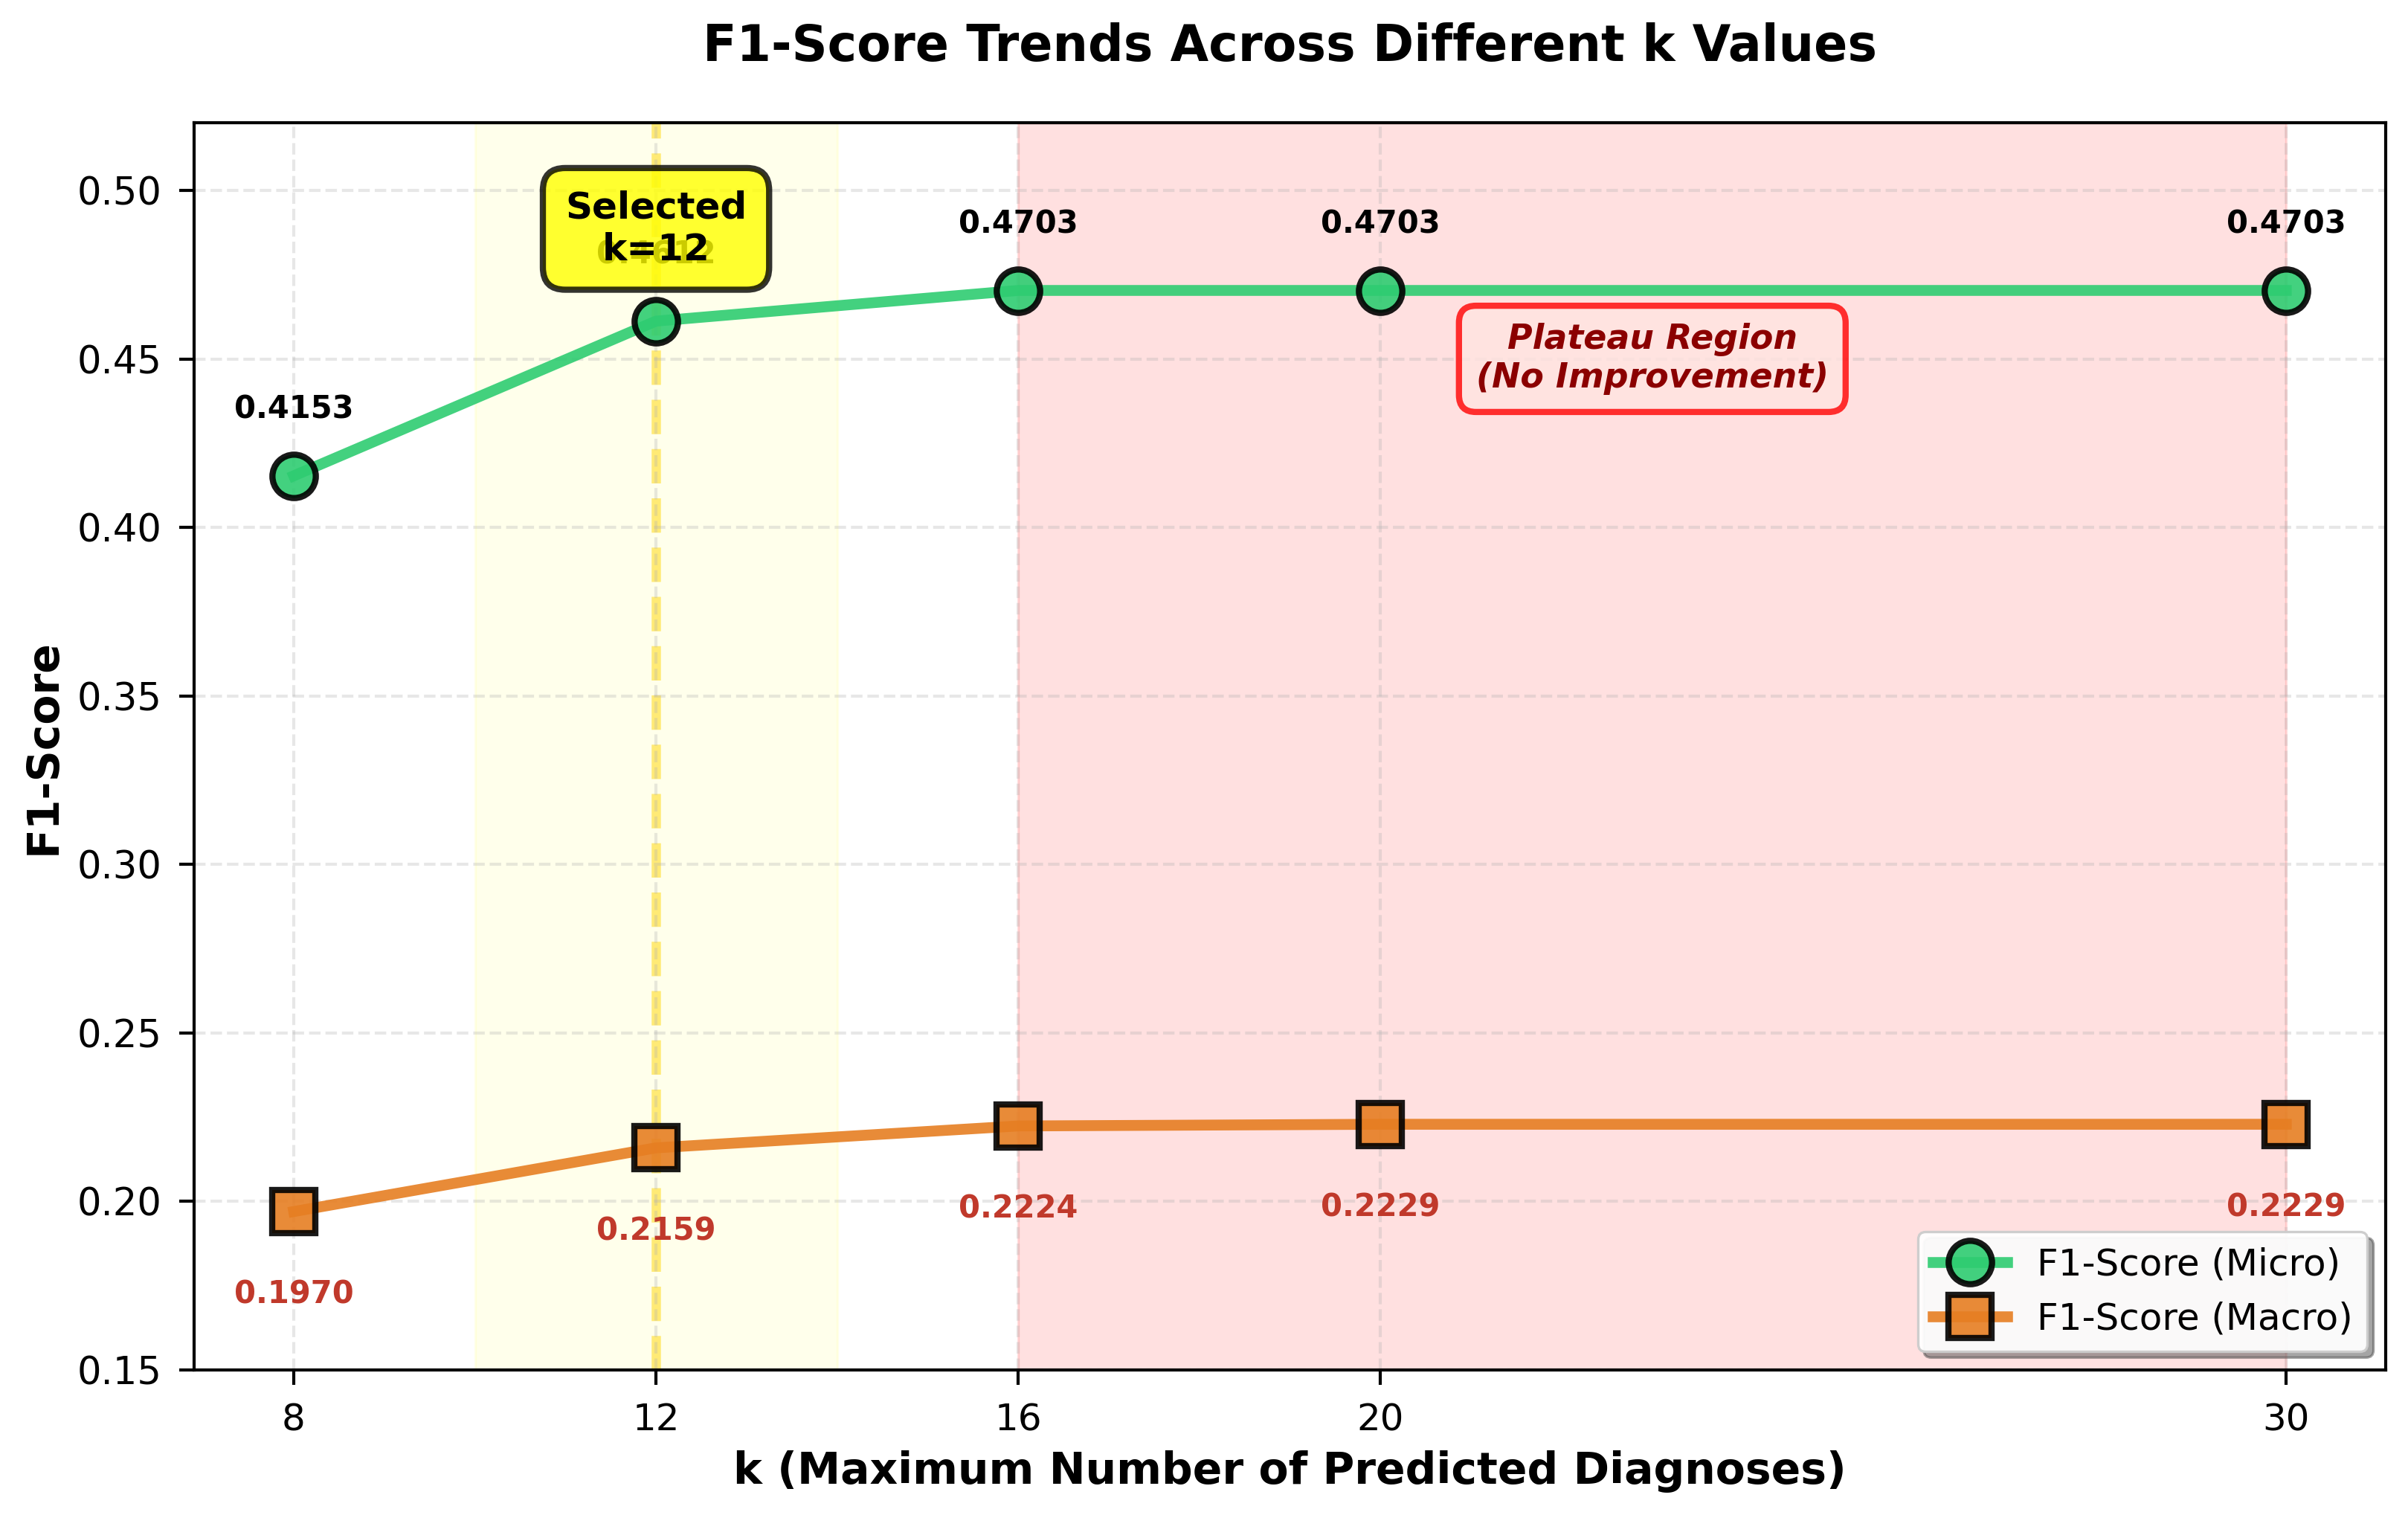
\includegraphics[width=\textwidth]{Images/k_ablation_f1_trends.png}
%         \caption{F1 trends (Micro/Macro) vs.\ \(k\)}
%         \label{fig:k_f1_trends}
%     \end{subfigure}
%     \hfill
%     \begin{subfigure}[b]{0.32\textwidth}
%         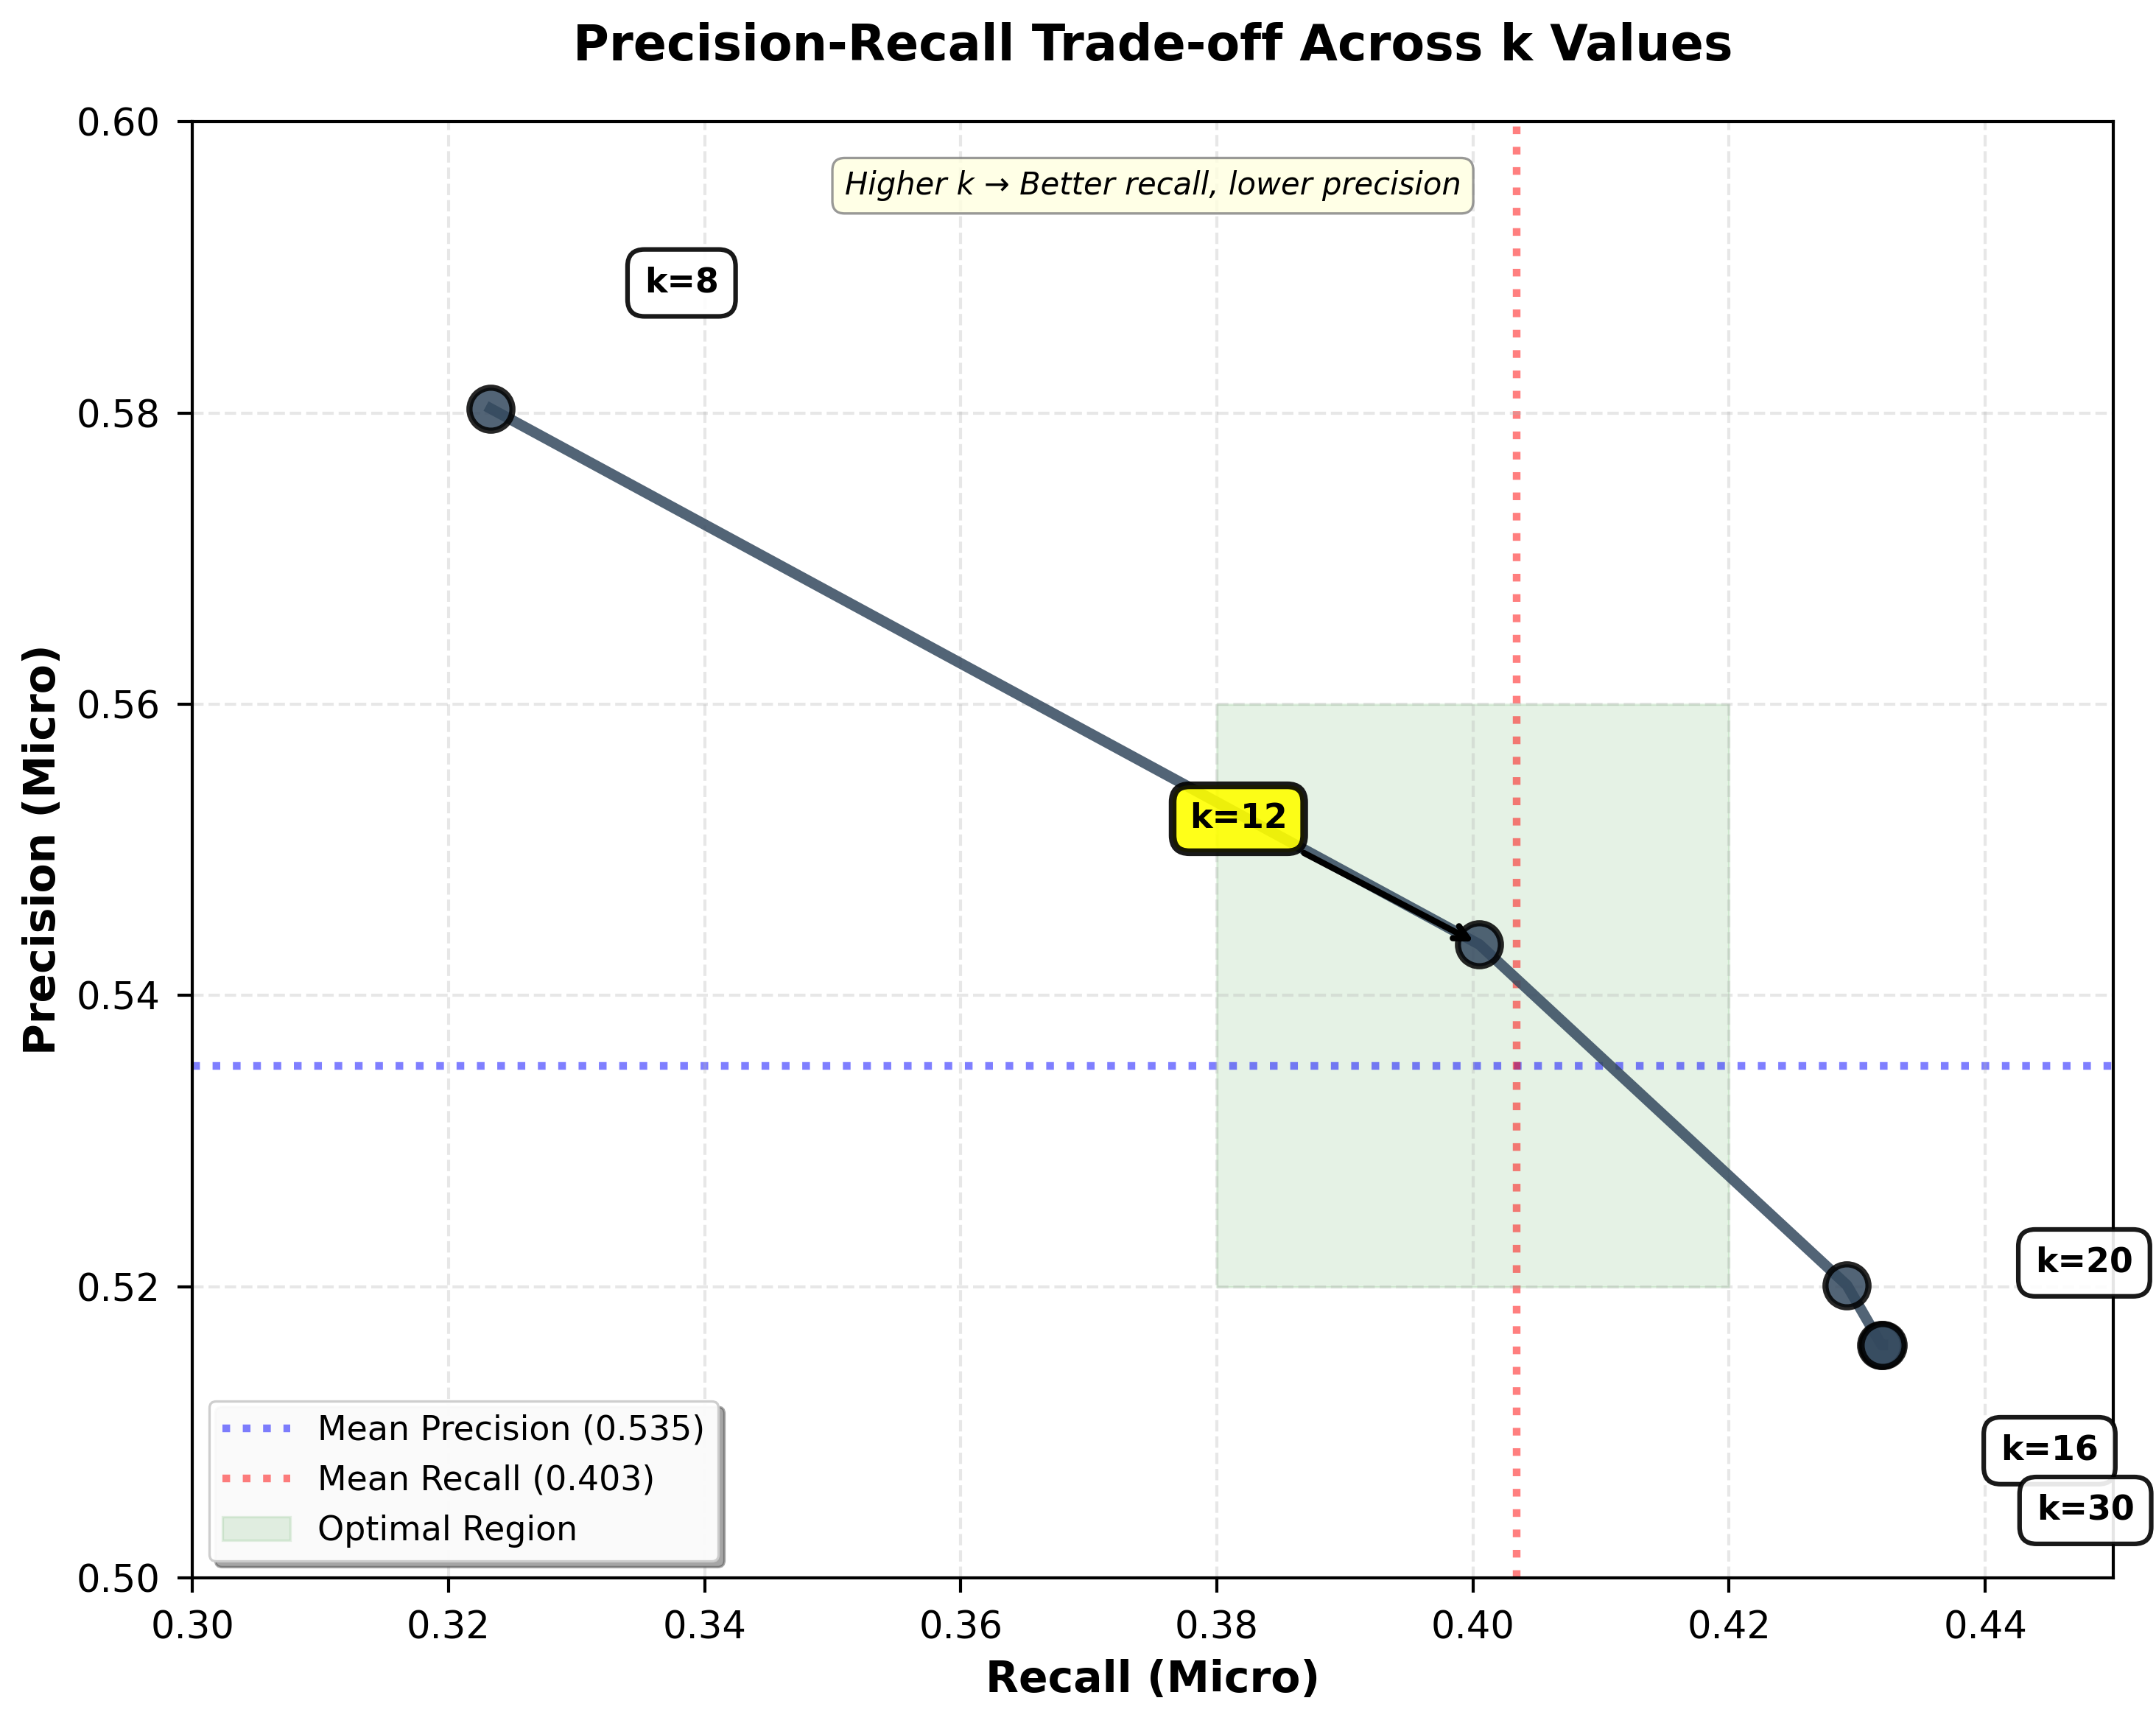
\includegraphics[width=\textwidth]{Images/k_ablation_precision_recall.png}
%         \caption{Precision--recall trade-off}
%         \label{fig:k_pr_tradeoff}
%     \end{subfigure}
%     \hfill
%     \begin{subfigure}[b]{0.32\textwidth}
%         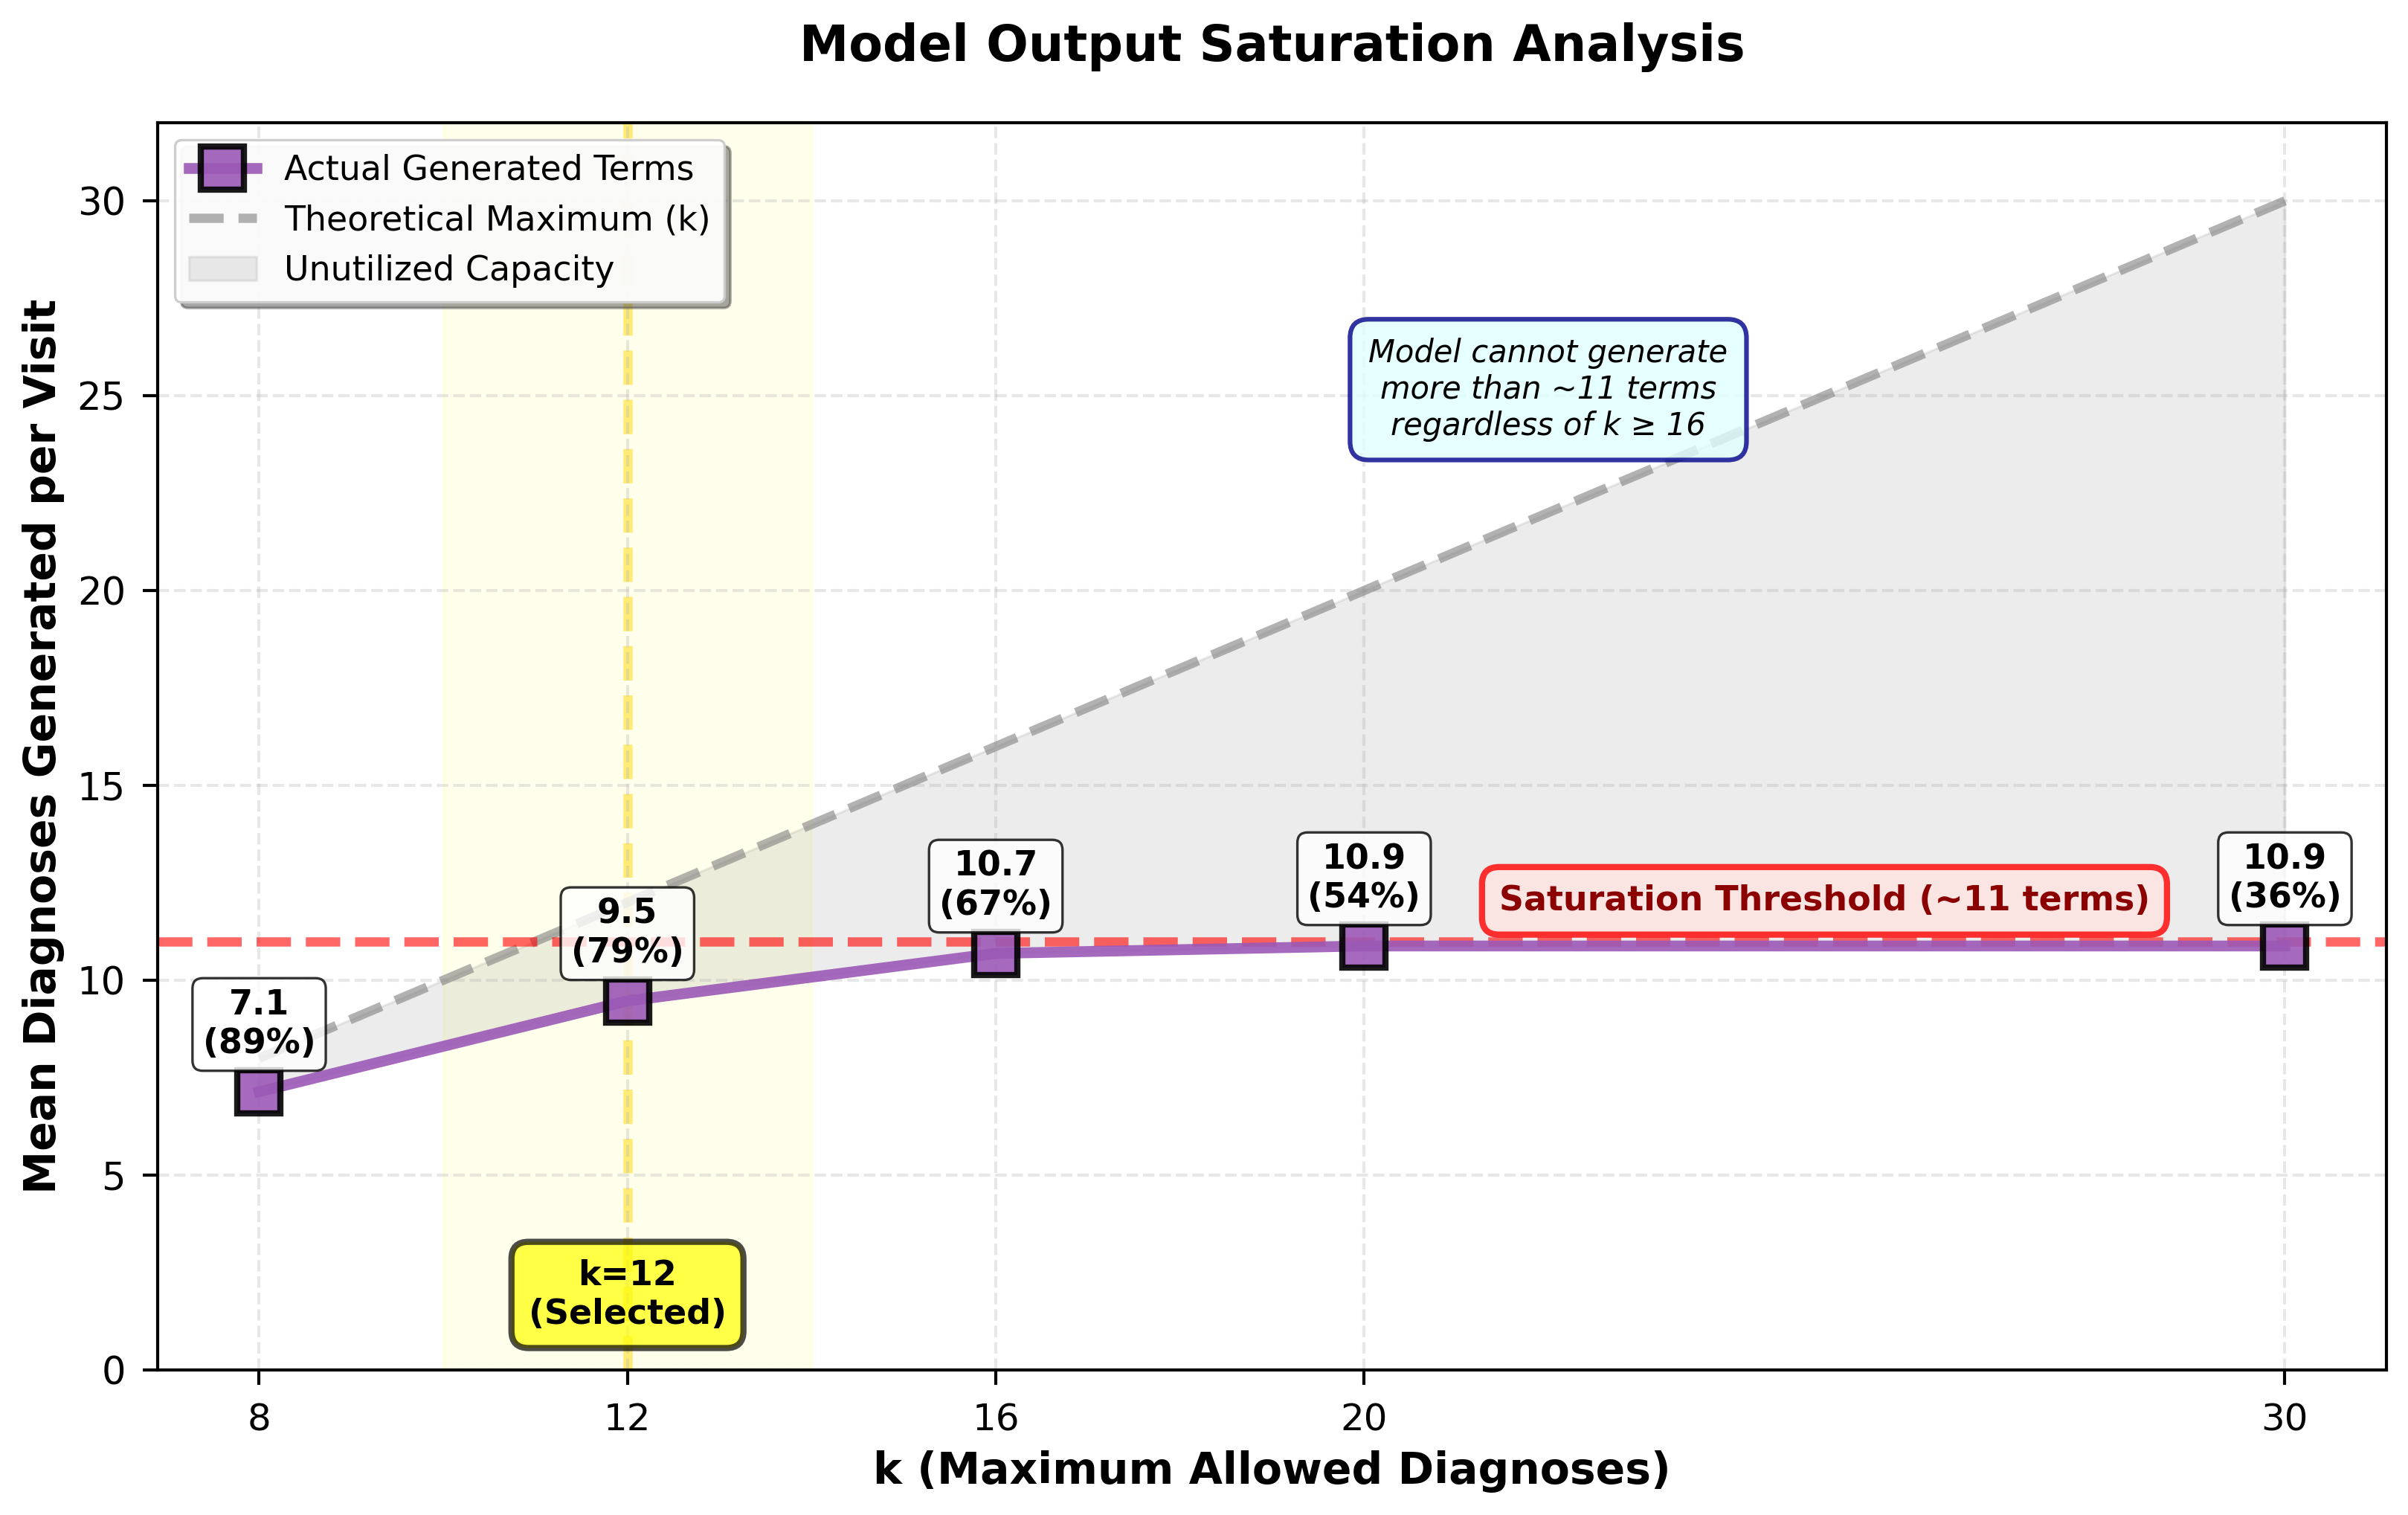
\includegraphics[width=\textwidth]{Images/k_ablation_saturation.png}
%         \caption{Mean terms/visit and saturation}
%         \label{fig:k_saturation}
%     \end{subfigure}
%     \caption{\textbf{K-ablation study.} Increasing \(k\) improves performance up to \(k=16\), after which metrics plateau. The precision--recall curve highlights the trade-off as \(k\) increases, while the mean predicted terms/visit saturate, indicating limited benefit from larger output budgets.}
%     \label{fig:k_ablation}
% \end{figure*}


% % ============================================================
% \subsection{Summary, Improvements, and Transition}
% \label{subsec:results-task1-summary}

% Task~1 results form a coherent progression:
% \begin{itemize}
%     \item \textbf{Strong baseline:} fine-tuned TextGen provides a clean and competitive reference point compared to Base and CodeGen.
%     \item \textbf{Inference-only KG ablation:} injecting KG paths at inference without KG-aware training does not reliably improve performance and often degrades it, consistent with the hypothesis that na\"ive KG injection can introduce noise and distract generation.
%     \item \textbf{KG-augmented fine-tuning helps:} RAG-style variants produce consistent gains over the best baseline across overall, parent-level, and frequency-sliced evaluation, with the most meaningful improvements observed on Tail-50 codes.
% \end{itemize}

% To make improvements explicit, Table~\ref{tab:task1-delta-summary-final} summarises absolute ($\Delta$) and relative (\%) gains from Baseline TextGen (no KG at inference) to the best KG-augmented variant per backbone (chosen by overall micro-F1; Tail-50 best variants may differ).

% \begin{table}[t]
% \centering
% \caption{Improvements from Baseline TextGen (no KG at inference) to best KG-augmented variant per backbone. Relative gains shown as percent.}
% \label{tab:task1-delta-summary-final}
% \resizebox{\textwidth}{!}{
% \begin{tabular}{lcccccc}
% \toprule
% \textbf{Backbone} &
% \textbf{Overall micro-F1} & $\Delta$ (\%) &
% \textbf{Overall macro-F1} & $\Delta$ (\%) &
% \textbf{Tail-50 micro-F1} & $\Delta$ (\%) \\
% \midrule
% Llama-3.2-1B &
% 0.4313 $\rightarrow$ 0.4749 & +0.0436 (+10.1\%) &
% 0.2065 $\rightarrow$ 0.2368 & +0.0303 (+14.7\%) &
% 0.1429 $\rightarrow$ 0.1841 & +0.0412 (+28.8\%) \\
% \midrule
% Llama-3.1-8B &
% 0.4585 $\rightarrow$ 0.5029 & +0.0444 (+9.7\%) &
% 0.2457 $\rightarrow$ 0.2762 & +0.0305 (+12.4\%) &
% 0.1250 $\rightarrow$ 0.1820 & +0.0570 (+45.6\%) \\
% \midrule
% Meditron3-8B &
% 0.4556 $\rightarrow$ 0.5036 & +0.0480 (+10.5\%) &
% 0.2457 $\rightarrow$ 0.2793 & +0.0336 (+13.7\%) &
% 0.1304 $\rightarrow$ 0.1915 & +0.0611 (+46.9\%) \\
% \bottomrule
% \end{tabular}}
% \end{table}

\section{Task~1: Current-Visit Diagnosis Prediction}
\label{sec:results-task1}

This section reports results for Task~1 (current-visit diagnosis prediction) under the evaluation protocol in Section~\ref{sec:evaluation}. We evaluate three modelling stages (\textbf{Base}, \textbf{CodeGen}, \textbf{TextGen}) across three backbones (\texttt{Llama-3.2-1B-Instruct}, \texttt{Llama-3.1-8B-Instruct}, \texttt{Meditron-8B}). 
For \textbf{Base} runs, LoRA adapters are disabled (no task-specific updates). For \textbf{CodeGen} and \textbf{TextGen}, the backbones are fine-tuned with LoRA using the prompts defined in Section~\ref{sec:model-architectures}. 

We then study whether structured knowledge improves TextGen via two steps:
(i) an \textbf{inference-only KG ablation} where KG paths are injected at test time without changing training, and
(ii) \textbf{KG-augmented fine-tuning (RAG-style)} where the model is trained to use KG paths (and also receives them at inference).
This ordering is intentional: it isolates whether KG helps only when the model is explicitly trained to leverage it.

As described in Section~\ref{subsec:complexity-cohort}, all models are instructed to generate a fixed budget of \textbf{at most 12 diagnoses per admission}. This interacts non-trivially with recall in highly multimorbid admissions: improvements in recall often require \emph{better prioritisation} under a limited output budget rather than simply generating more outputs.

% ============================================================
\subsection{Baseline Performance: From Raw Backbones to Fine-Tuned Pipelines}
\label{subsec:results-task1-baselines}

Before analysing knowledge augmentation, we quantify how well the raw instruction-tuned backbones perform on Task~1 without task-specific fine-tuning. In these \emph{Base} runs, models are used ``as is'' with the same Task~1 prompts (Section~\ref{sec:model-architectures}), but LoRA adapters are disabled. This establishes a lower bound on performance and clarifies how much of the task is solved by generic instruction-following alone.

We evaluate four configurations per backbone:
\begin{enumerate}
    \item \textbf{Base (CodeGen):} raw backbone prompted to output ICD-9 codes directly (no fine-tuning).
    \item \textbf{CodeGen:} fine-tuned pipeline generating ICD-9 codes directly from multimodal prompts (Section~\ref{subsec:codegen-arch}).
    \item \textbf{Base (TextGen):} raw backbone prompted to output diagnosis terms (no fine-tuning), followed by SapBERT+FAISS mapping.
    \item \textbf{TextGen:} fine-tuned pipeline generating diagnosis terms followed by SapBERT+FAISS mapping (Section~\ref{subsec:textgen-arch}).
\end{enumerate}

Table~\ref{tab:task1-all-methods-flat} reports micro-F1 and macro-F1 at the full ICD-9 code level (test set). Precision/recall and sample-averaged metrics are visualised in Figure~\ref{fig:task1-flat-metrics}.

\begin{table}[t]
    \centering
    \caption{Task~1 (current-visit diagnosis prediction): comparison of raw backbones (\textbf{Base}), fine-tuned \textbf{CodeGen}, and fine-tuned \textbf{TextGen} across all backbones. Metrics are computed at the full ICD-9 code level on the held-out test set.}
    \label{tab:task1-all-methods-flat}
    \begin{tabular}{llcc}
        \toprule
        \textbf{Backbone} & \textbf{Method} &
        \textbf{Micro-F1} & \textbf{Macro-F1} \\
        \midrule
        \multirow{4}{*}{Llama-3.2-1B} 
            & Base (no FT) - Direct codes  & 0.0003 & 0.0000 \\
            & CodeGen        & 0.2344 & 0.0151 \\
            & Base (no FT) - Free Text  & 0.0393 & 0.0250 \\
            & TextGen        & \textbf{0.4313} & \textbf{0.2065} \\
        \midrule
        \multirow{4}{*}{Llama-3.1-8B} 
            & Base (no FT) - Direct codes  & 0.0269 & 0.0007 \\
            & CodeGen        & 0.2487 & 0.0188 \\
            & Base (no FT) - Free Text  & 0.0358 & 0.0244 \\
            & TextGen        & \textbf{0.4585} & \textbf{0.2457} \\
        \midrule
        \multirow{4}{*}{Meditron-8B} 
            & Base (no FT) - Direct codes  & 0.0040 & 0.0000 \\
            & CodeGen        & 0.2475 & 0.0186 \\
            & Base (no FT) - Free Text  & 0.0068 & 0.0071 \\
            & TextGen        & \textbf{0.4556} & \textbf{0.2457} \\
        \bottomrule
    \end{tabular}
\end{table}

Three consistent trends emerge:
\begin{itemize}
    \item \textbf{Raw backbones are insufficient.} Without fine-tuning, direct-code generation is near-zero across all backbones. Base TextGen is marginally better than Base CodeGen, suggesting models can sometimes produce plausible diagnosis language, but still cannot reliably recover a large multi-label ICD space.
    \item \textbf{Fine-tuning yields large, systematic gains.} Both CodeGen and TextGen improve substantially over their Base counterparts, confirming that task-specific supervision is essential for long clinical notes and highly imbalanced label spaces.
    \item \textbf{TextGen consistently outperforms CodeGen.} For every backbone, TextGen achieves higher micro-F1 and macro-F1 than CodeGen. The macro-F1 gap indicates better distribution of performance beyond the head labels, consistent with the design motivation of decoupling natural-language diagnosis generation from strict code formatting.
\end{itemize}

% --- KEEP THESE IMAGES EXACTLY (as requested) ---
\begin{figure}[t]
    \centering
    % Top row: micro-averaged metrics
    \begin{subfigure}{0.32\textwidth}
        \centering
        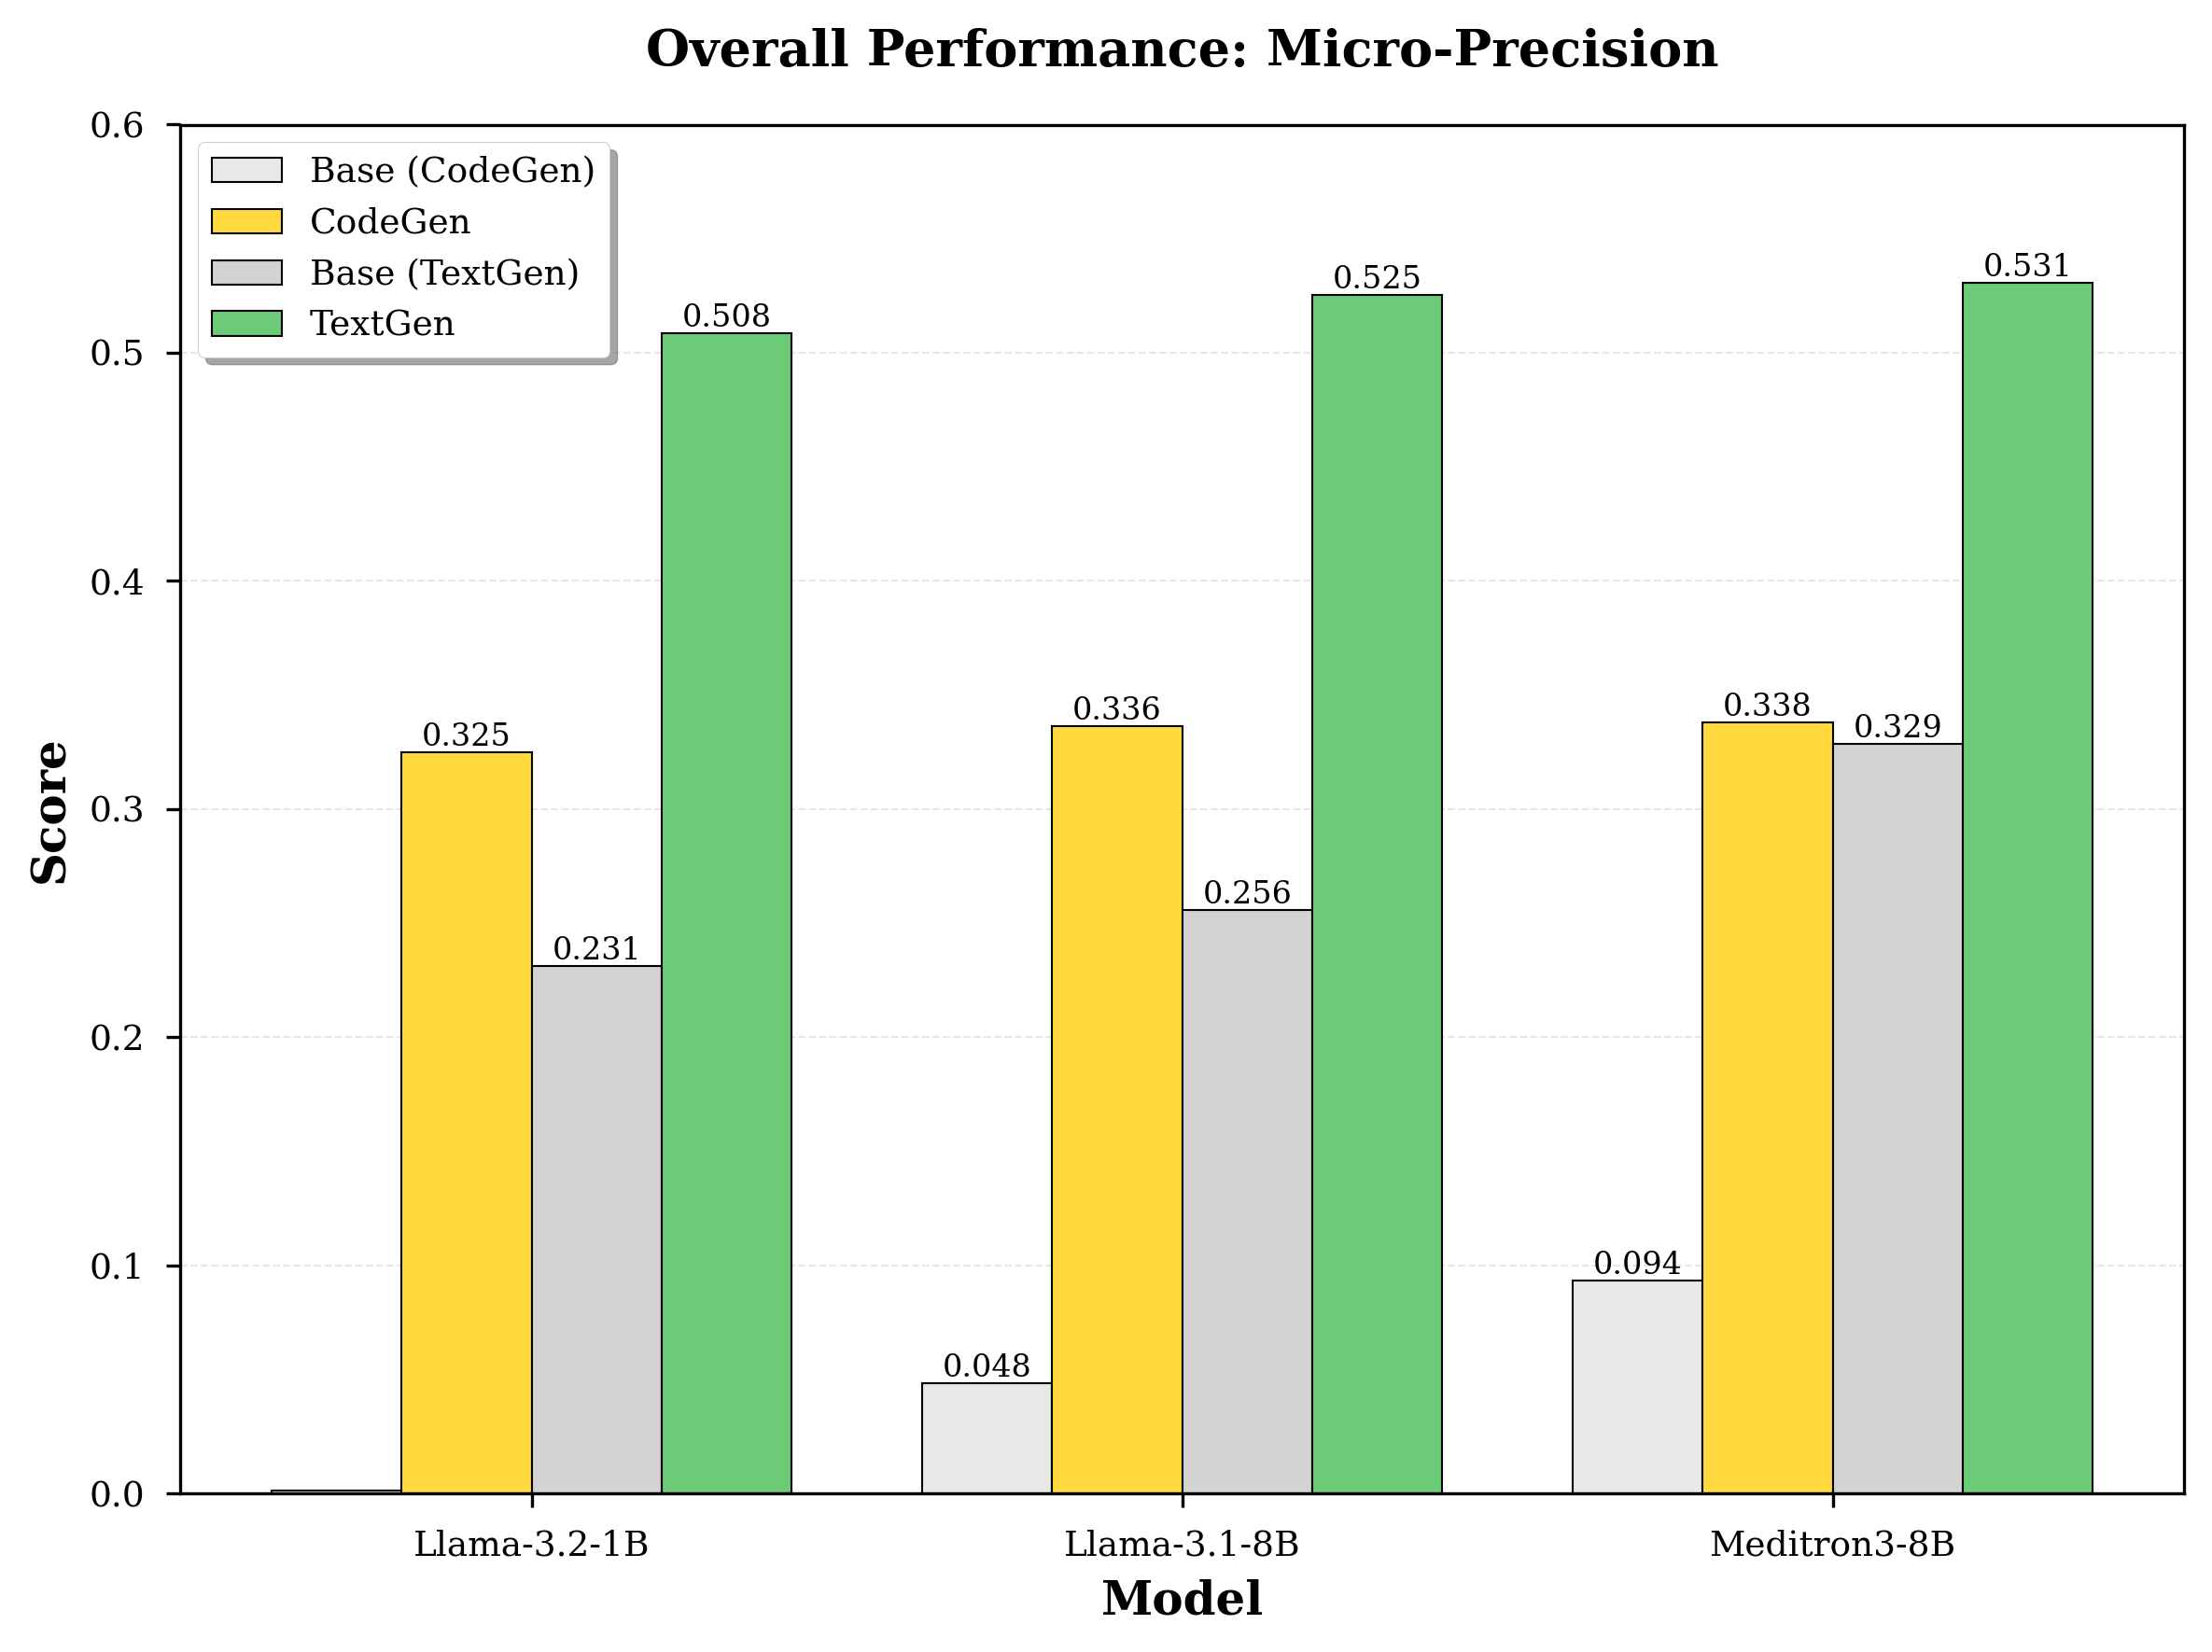
\includegraphics[width=\linewidth]{Images/Plots_thesis/overall_micro_precision.png}
        \caption{Micro-Precision}
        \label{fig:task1-flat-microP}
    \end{subfigure}\hfill
    \begin{subfigure}{0.32\textwidth}
        \centering
        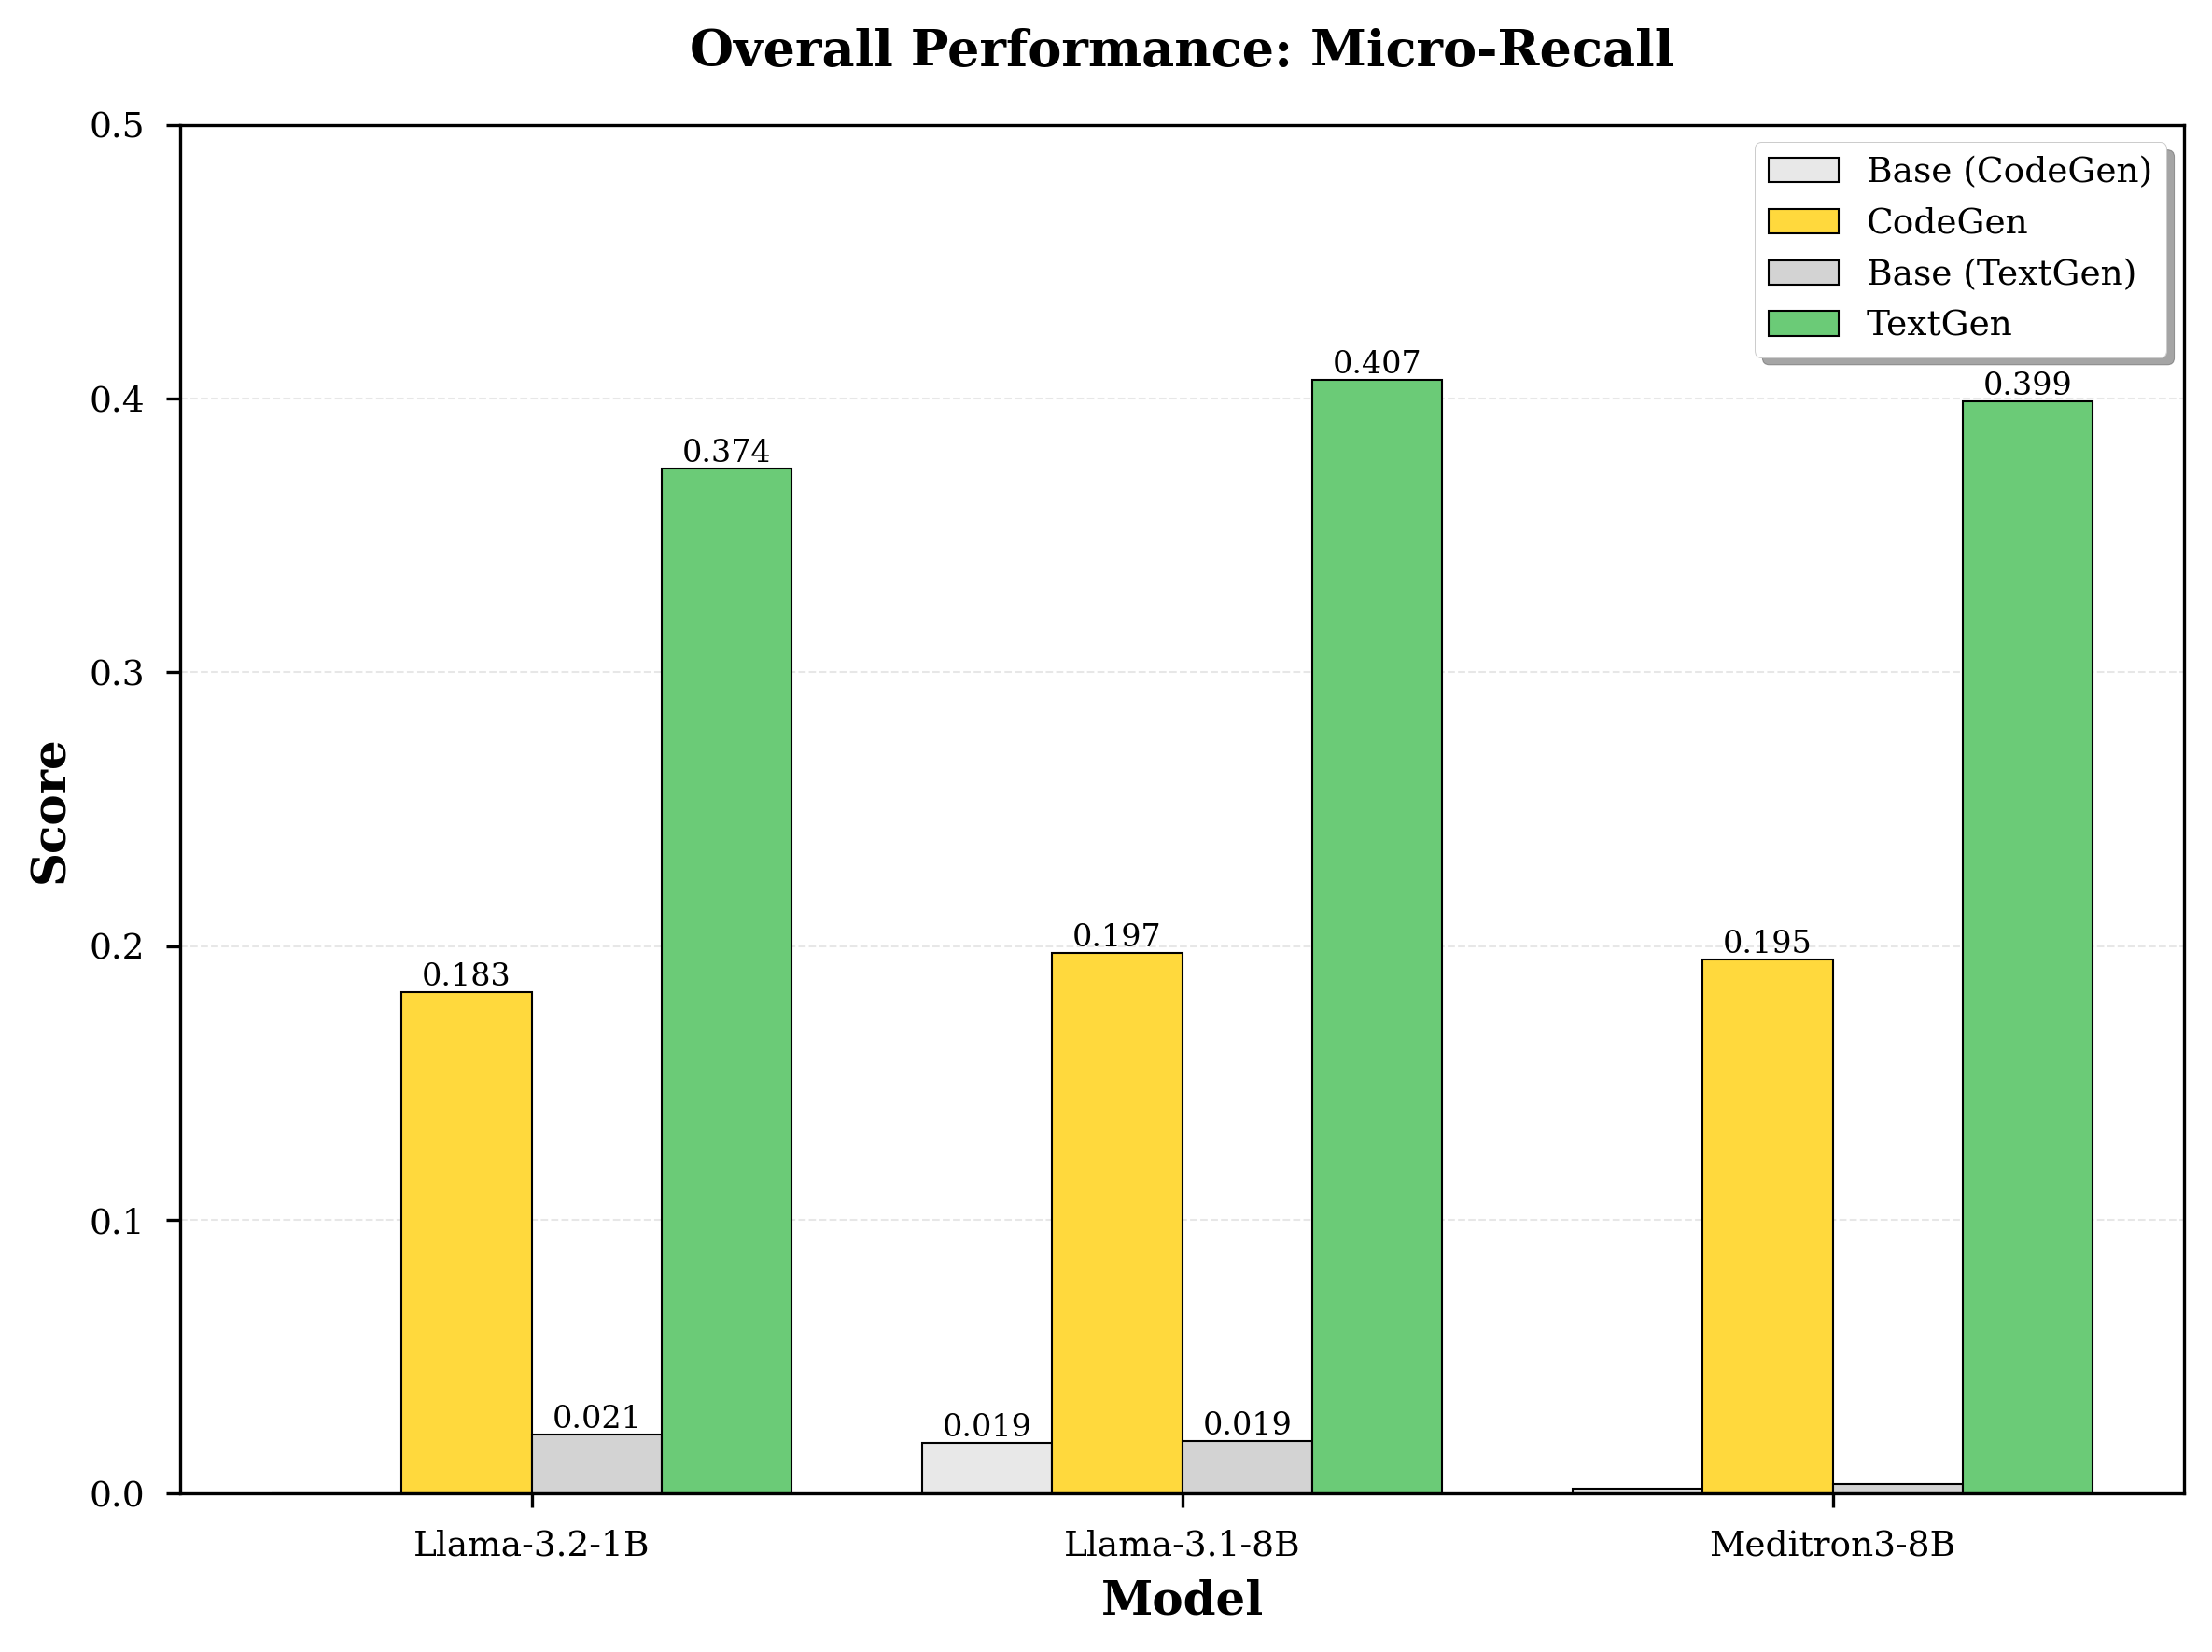
\includegraphics[width=\linewidth]{Images/Plots_thesis/overall_micro_recall.png}
        \caption{Micro-Recall}
        \label{fig:task1-flat-microR}
    \end{subfigure}\hfill
    \begin{subfigure}{0.32\textwidth}
        \centering
        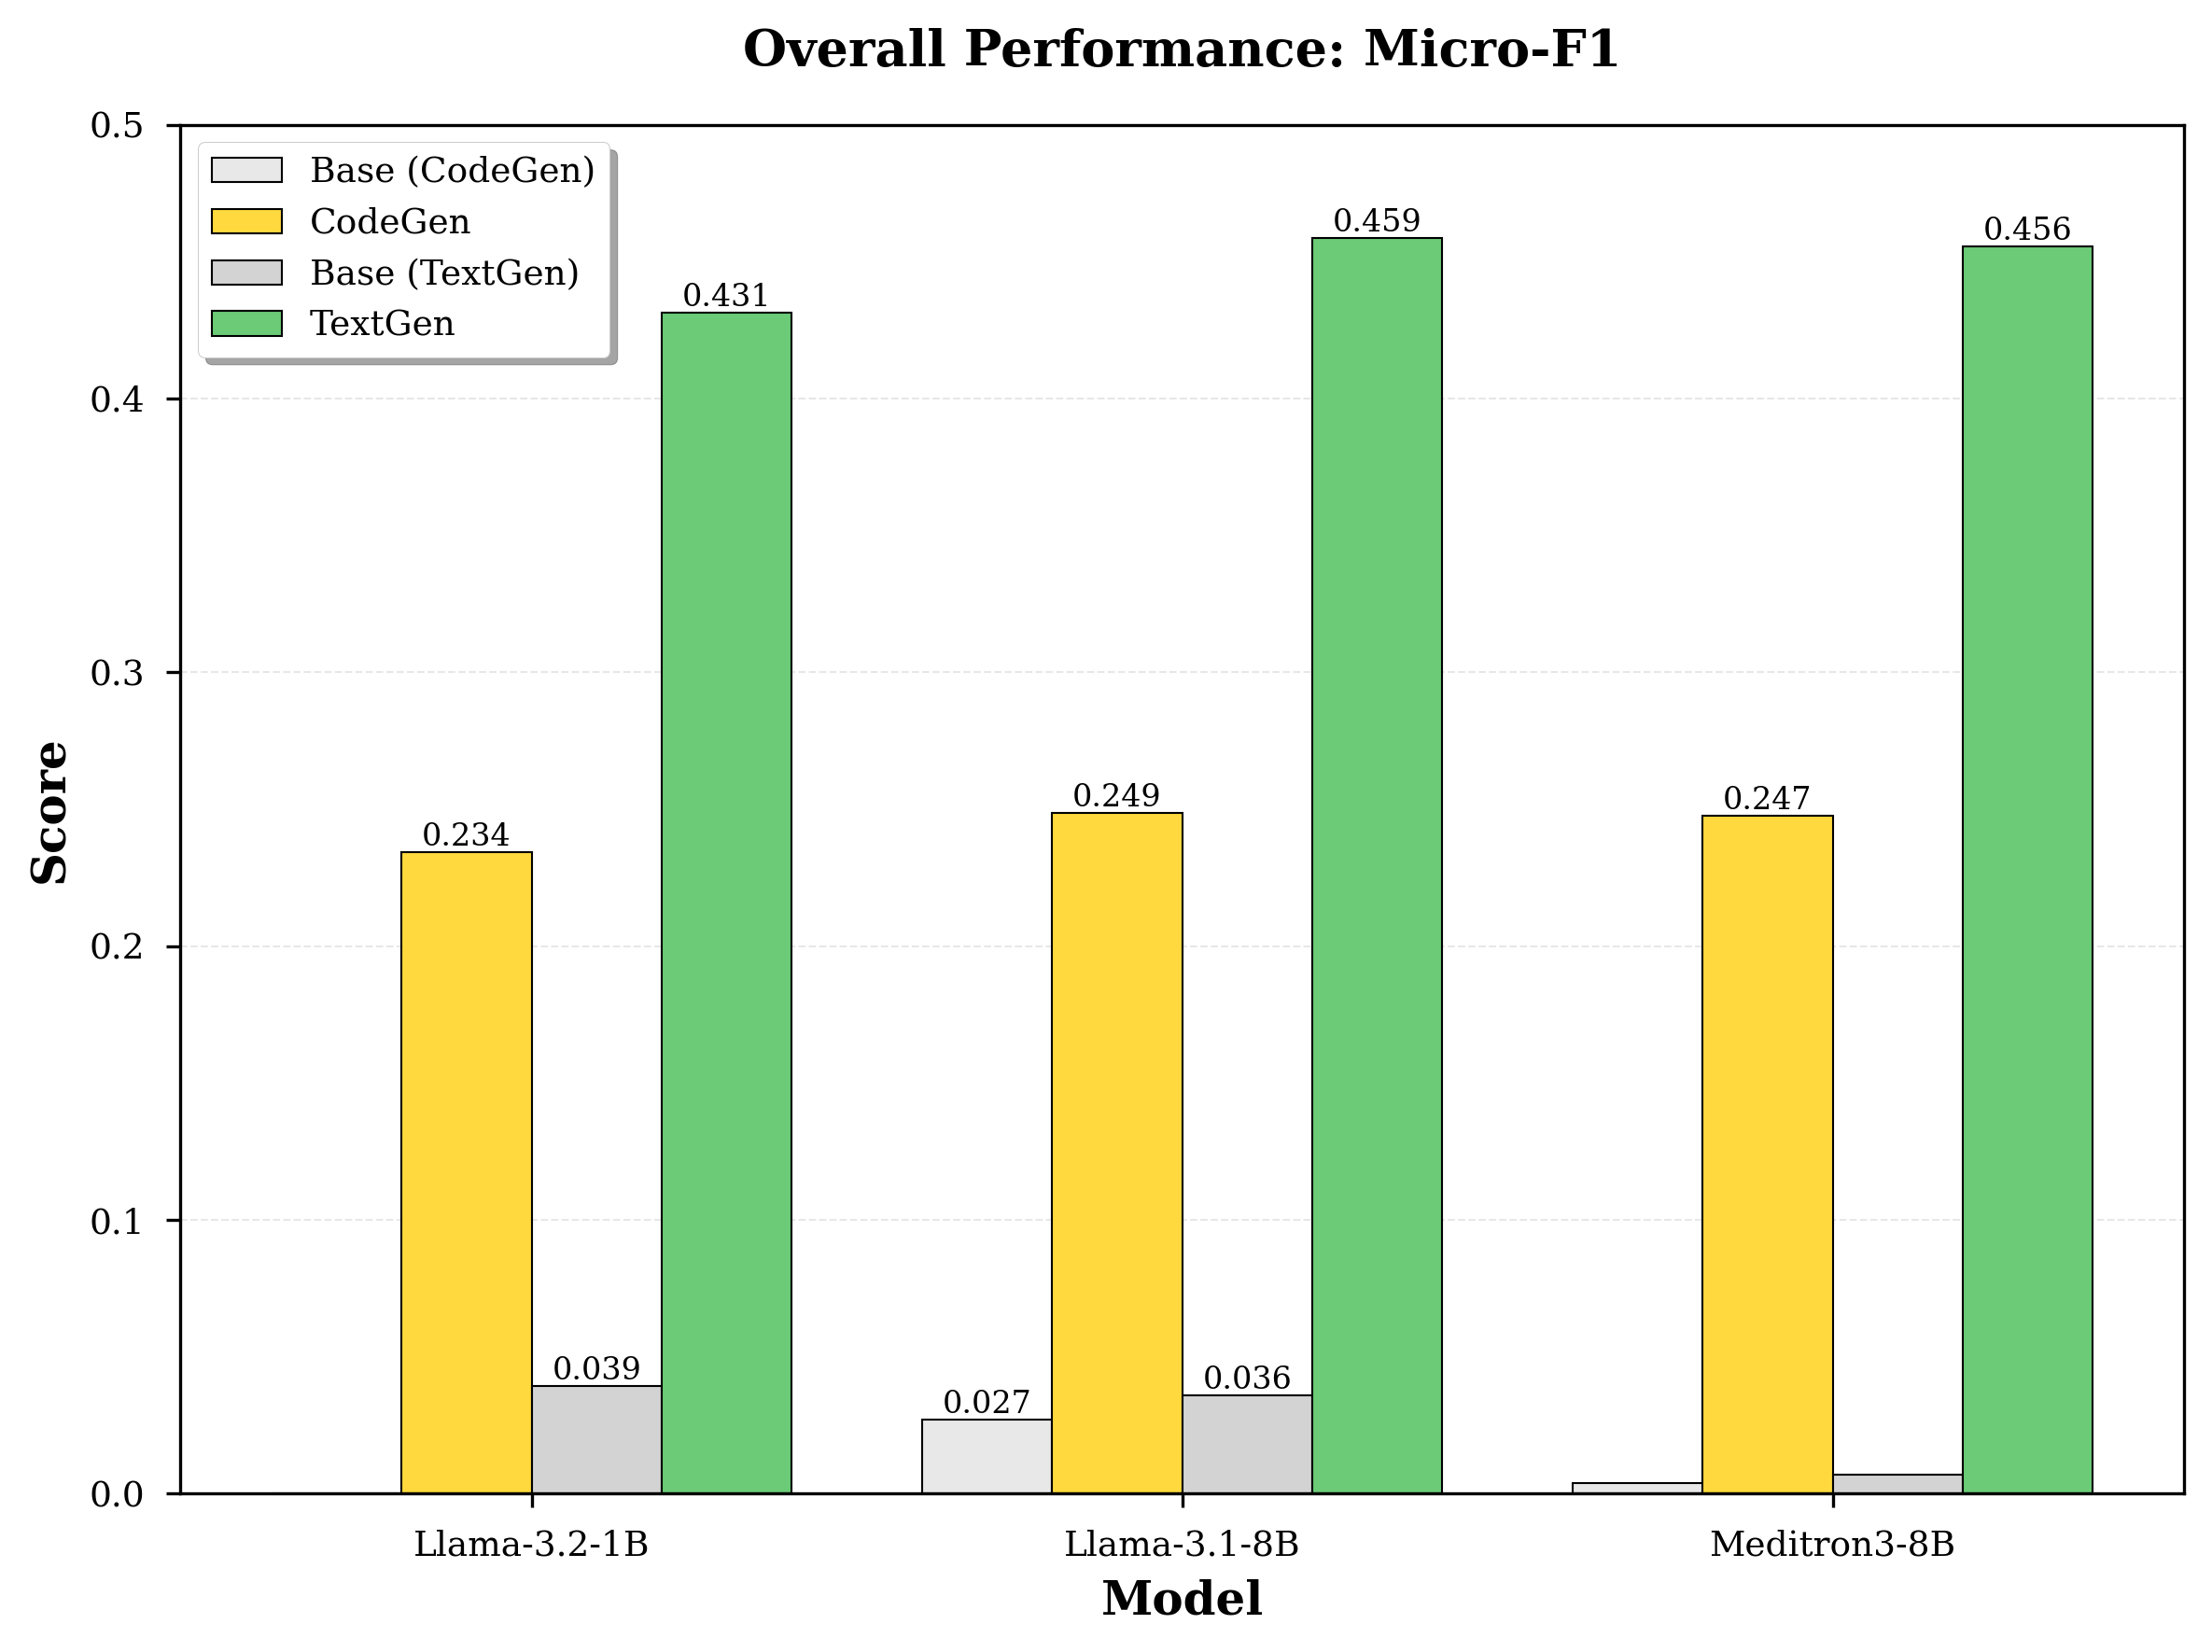
\includegraphics[width=\linewidth]{Images/Plots_thesis/overall_micro_f1.png}
        \caption{Micro-F1}
        \label{fig:task1-flat-microF1}
    \end{subfigure}

    \vspace{0.3cm}

    % Bottom row: macro-averaged metrics
    \begin{subfigure}{0.32\textwidth}
        \centering
        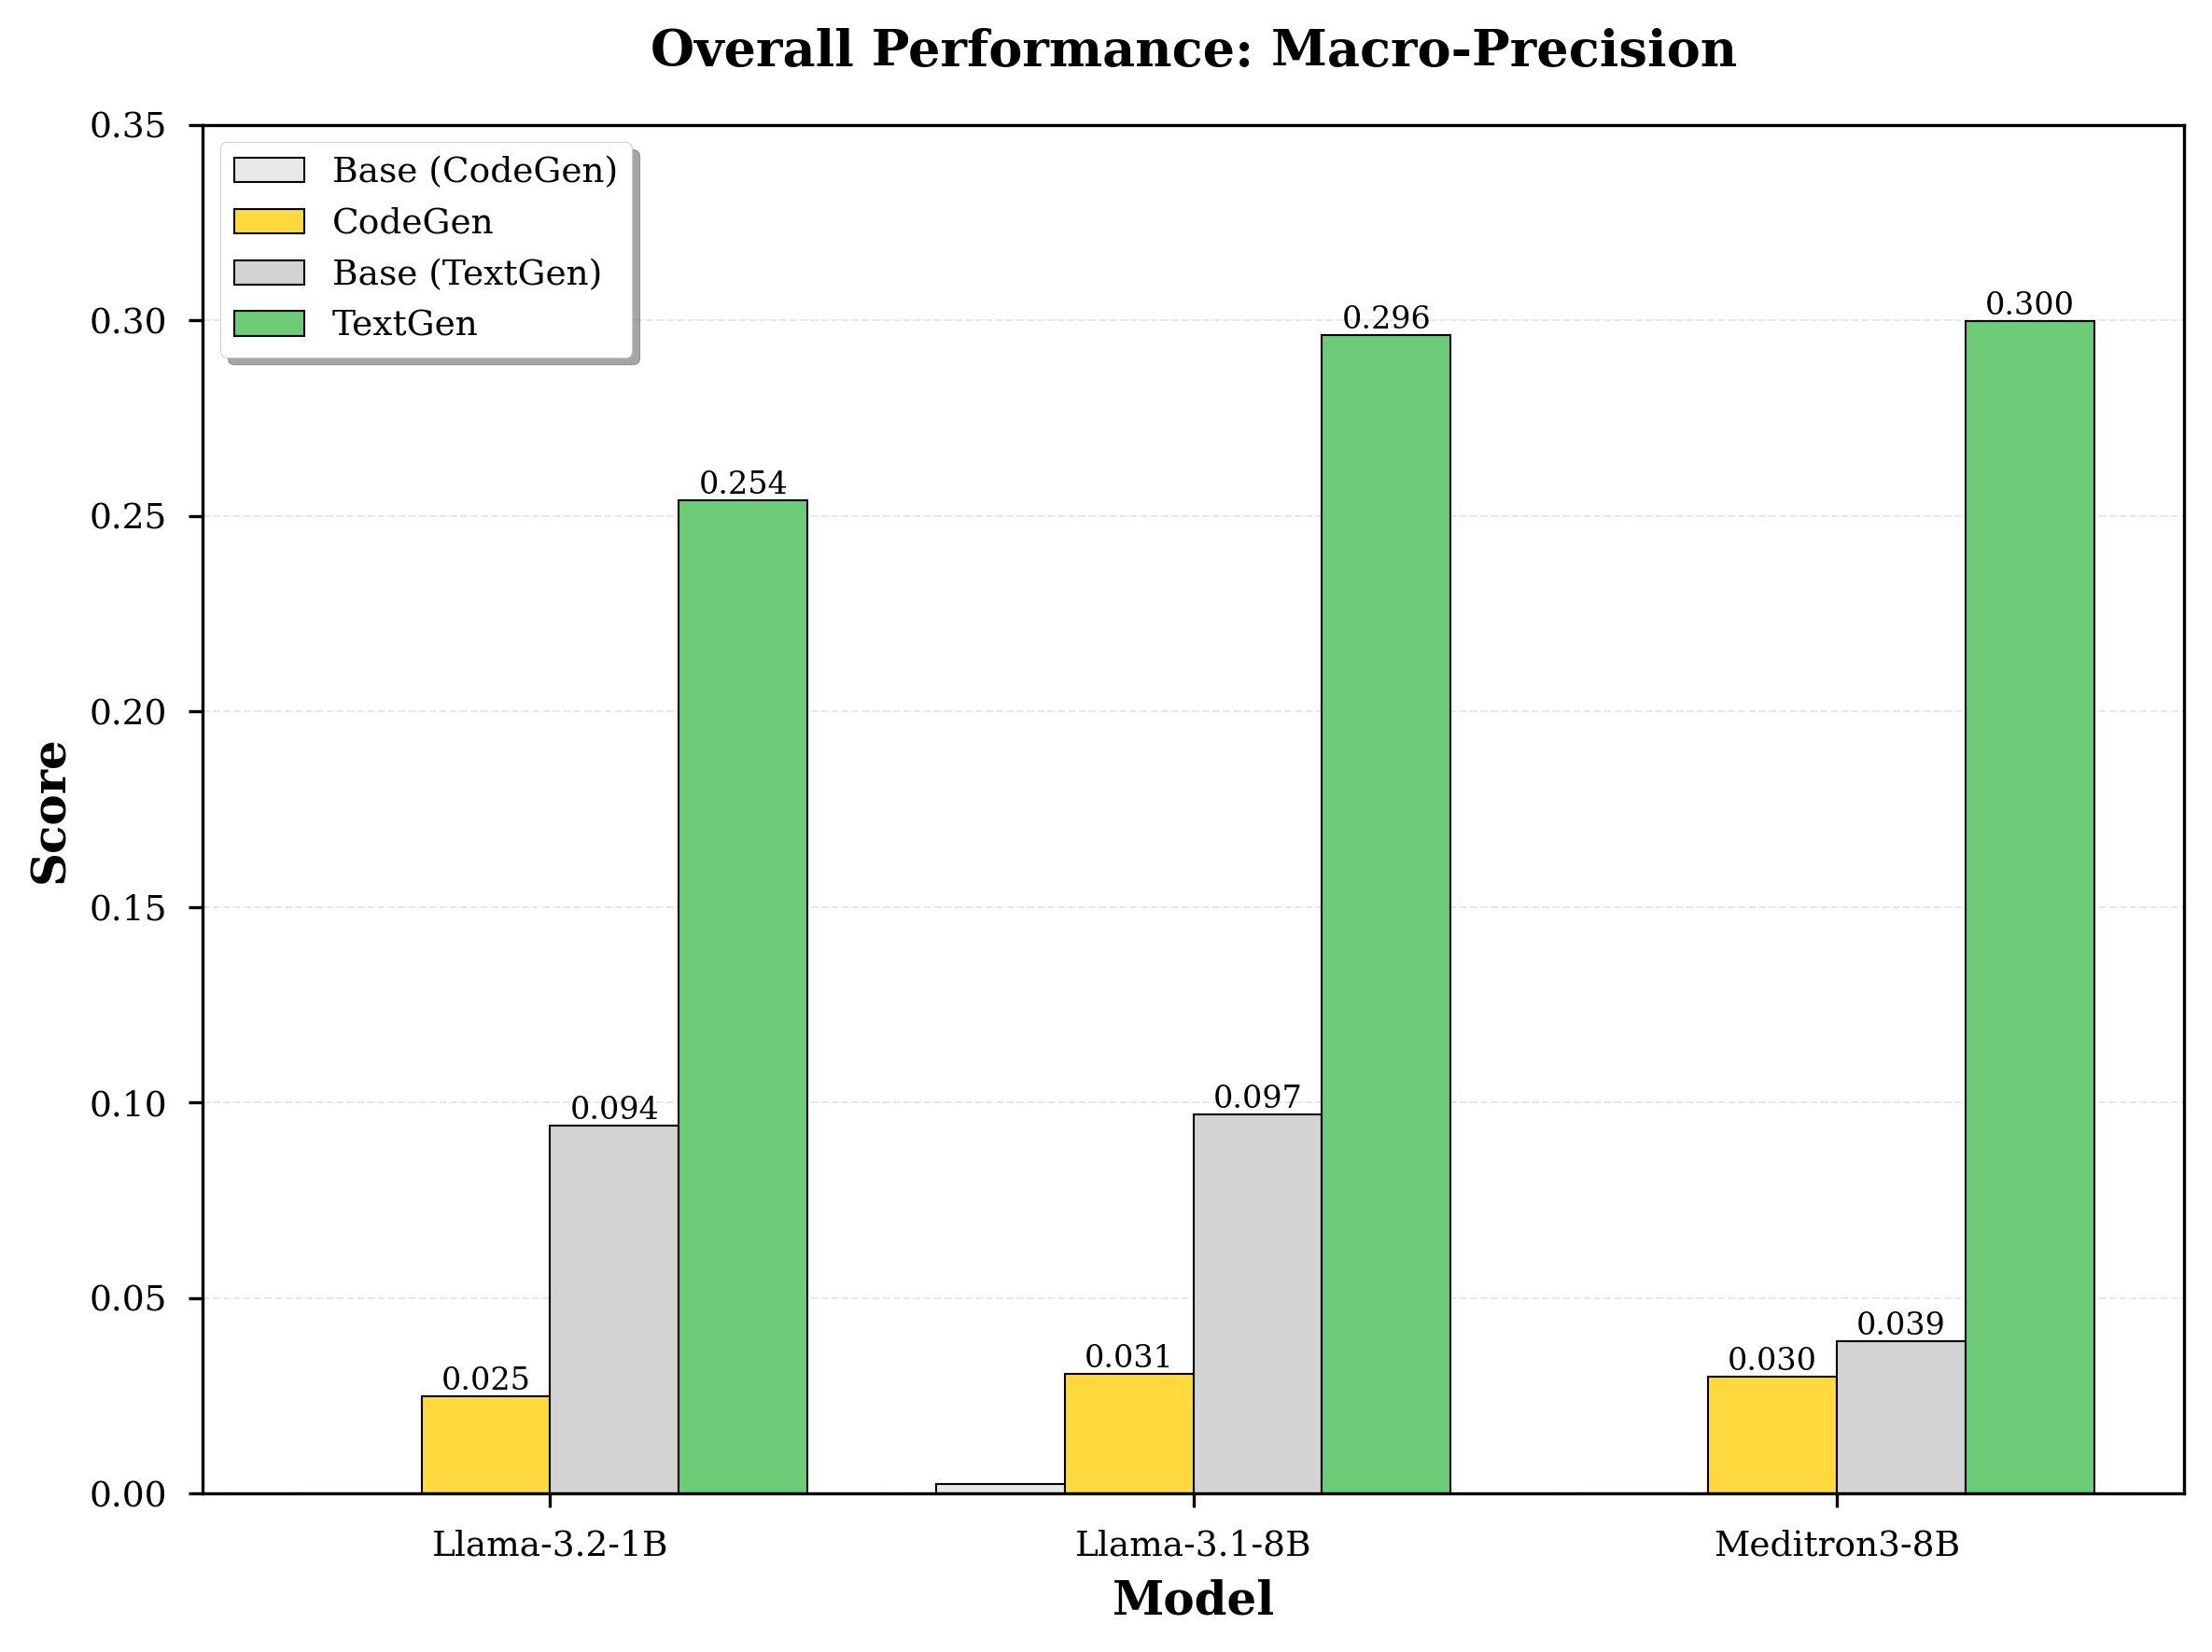
\includegraphics[width=\linewidth]{Images/Plots_thesis/overall_macro_precision.png}
        \caption{Macro-Precision}
        \label{fig:task1-flat-macroP}
    \end{subfigure}\hfill
    \begin{subfigure}{0.32\textwidth}
        \centering
        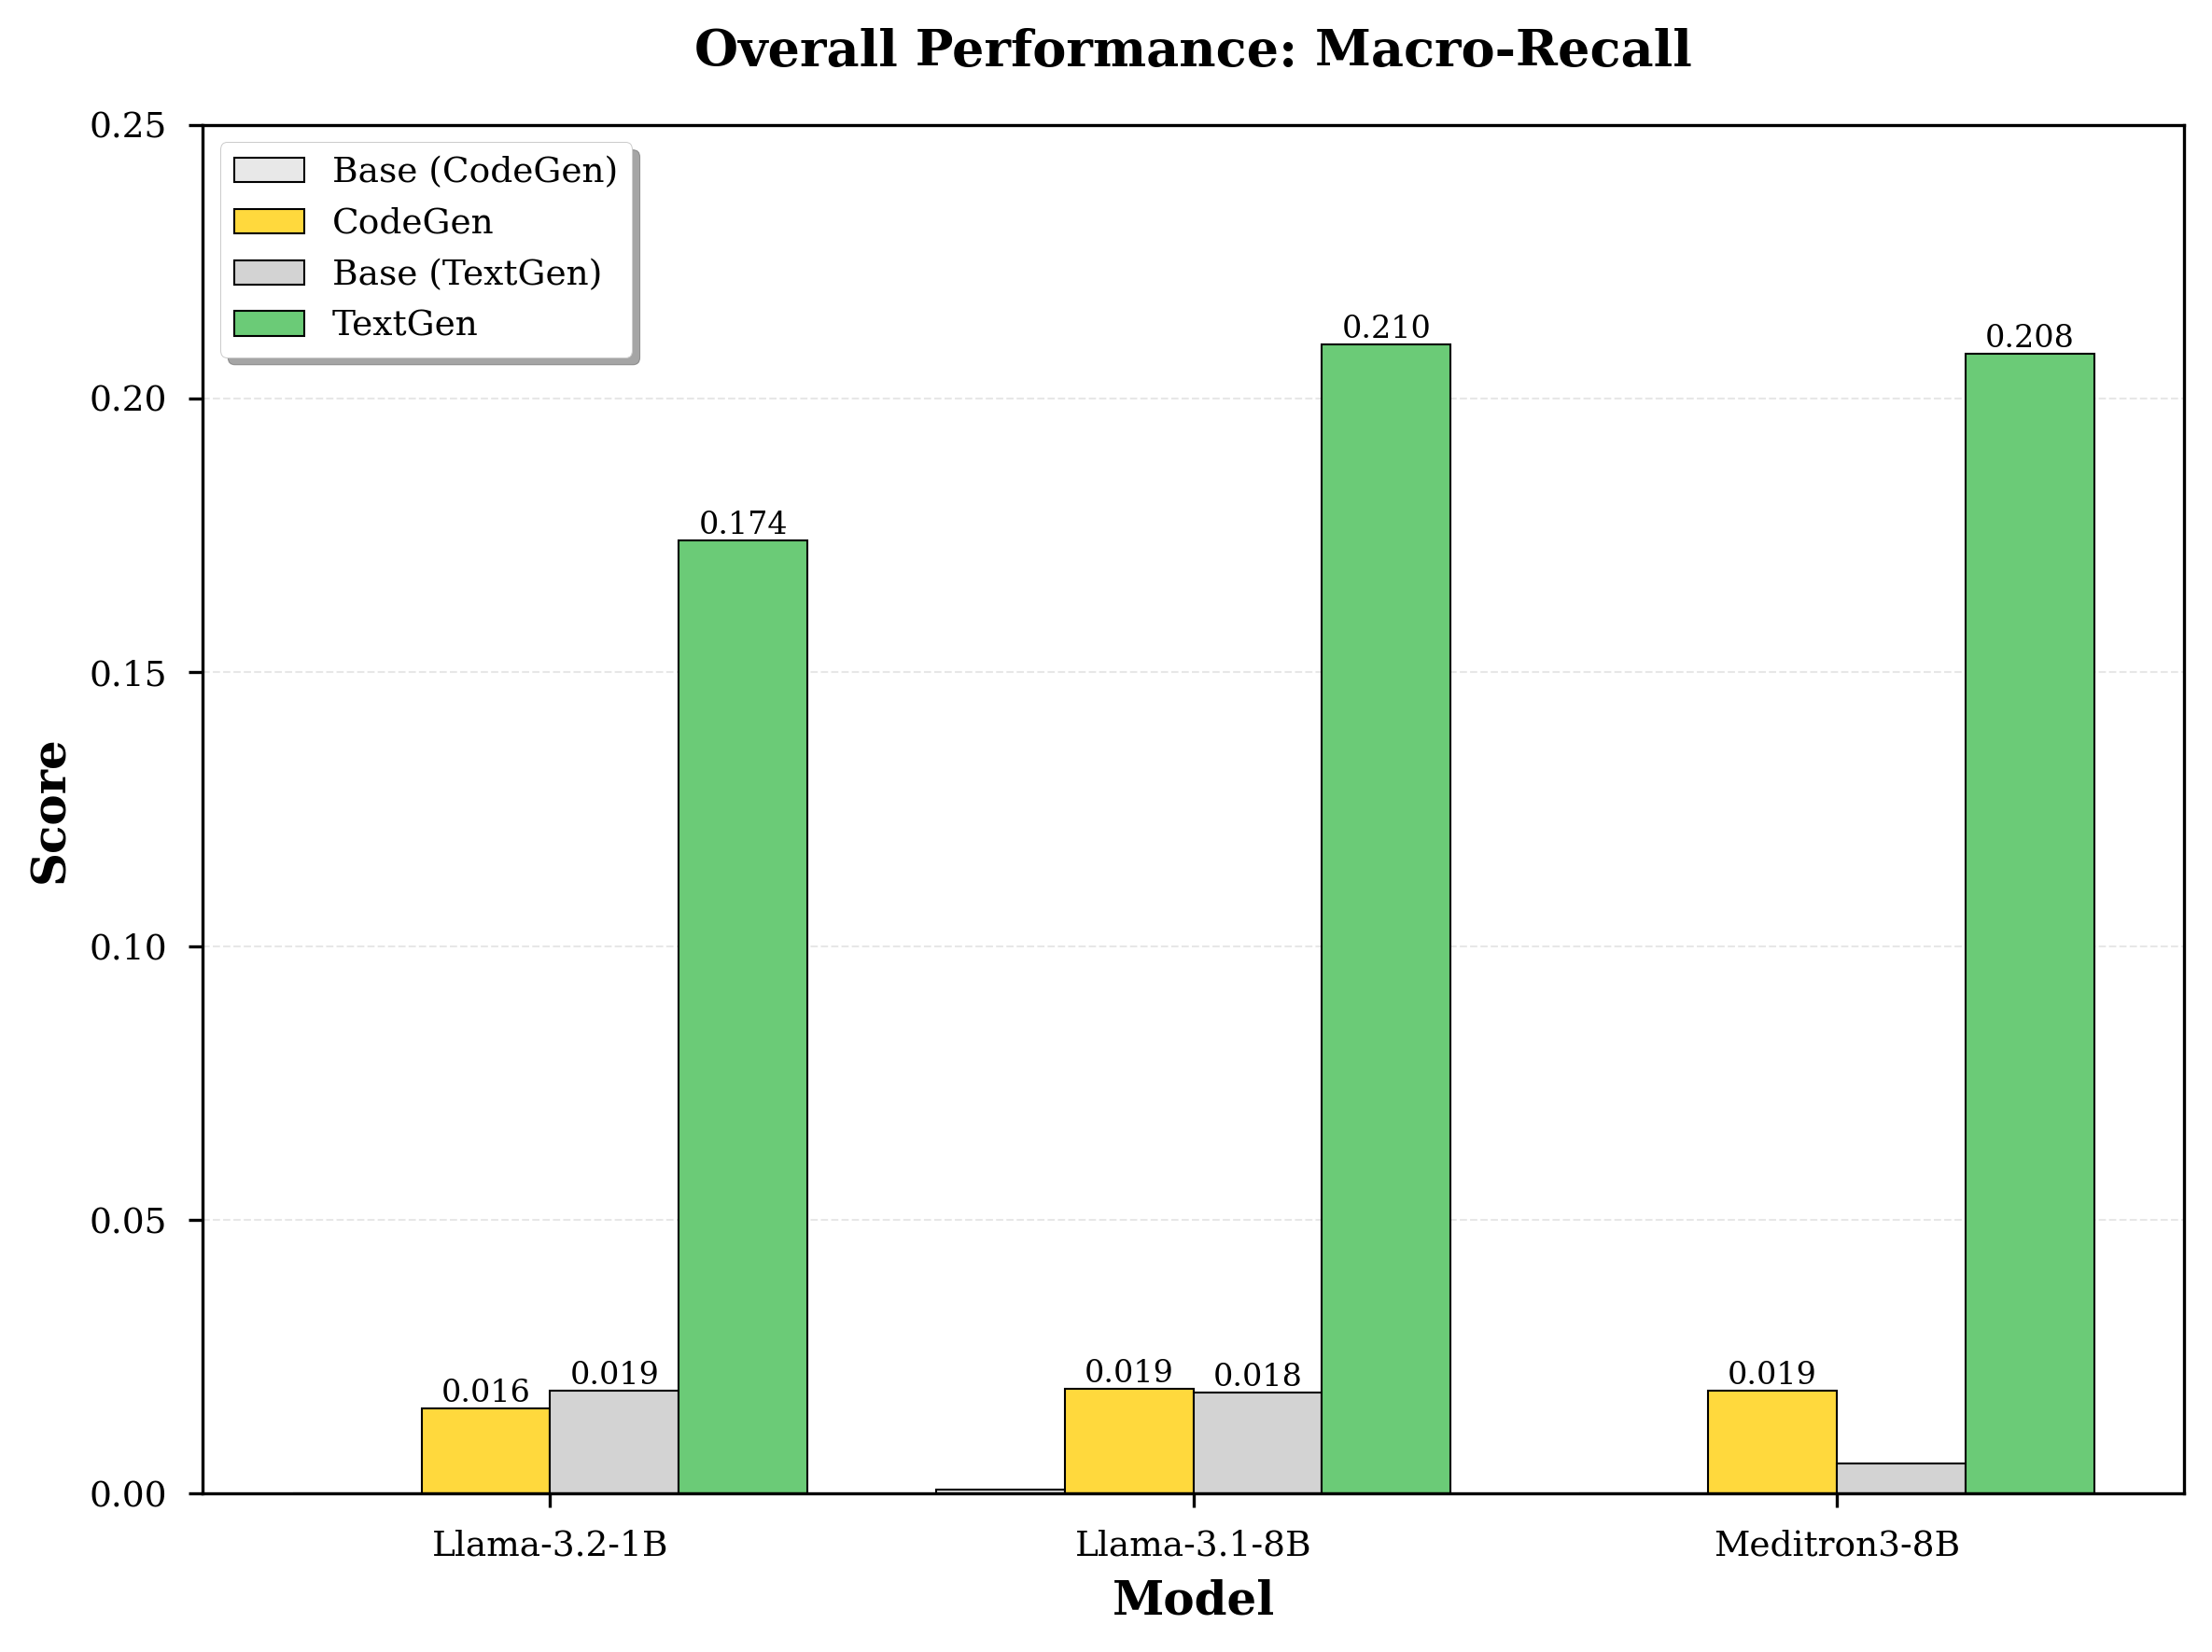
\includegraphics[width=\linewidth]{Images/Plots_thesis/overall_macro_recall.png}
        \caption{Macro-Recall}
        \label{fig:task1-flat-macroR}
    \end{subfigure}\hfill
    \begin{subfigure}{0.32\textwidth}
        \centering
        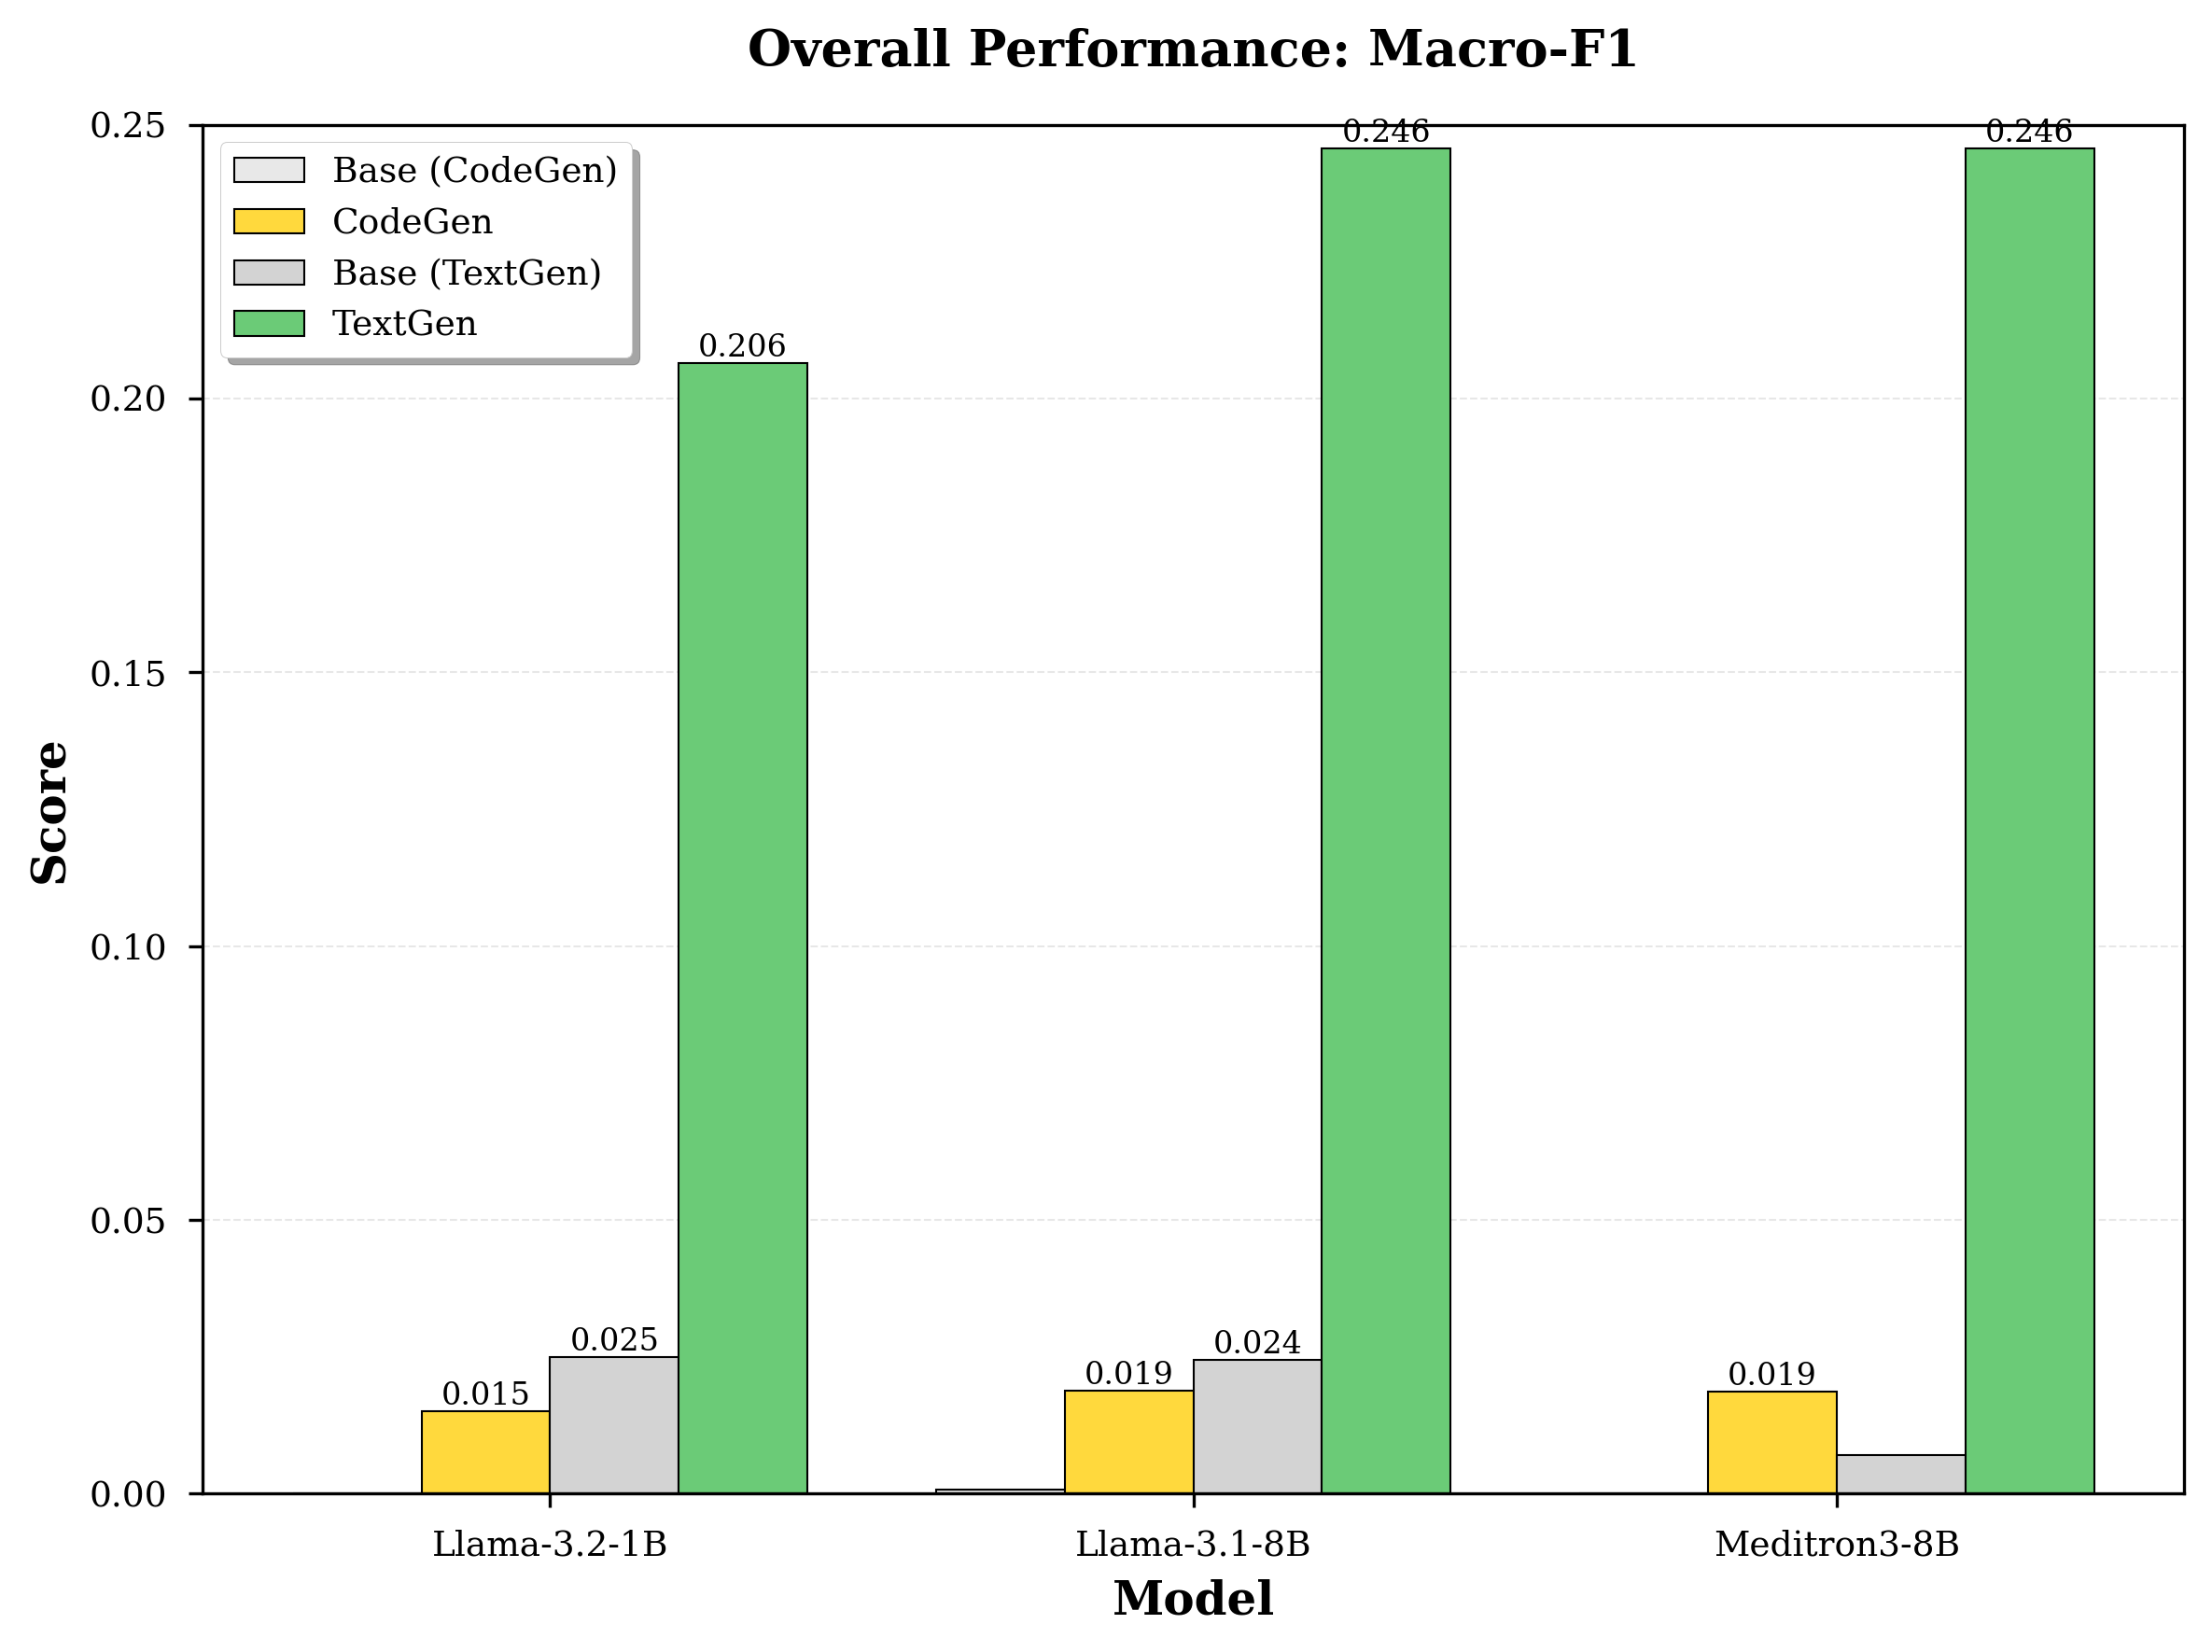
\includegraphics[width=\linewidth]{Images/Plots_thesis/overall_macro_f1.png}
        \caption{Macro-F1}
        \label{fig:task1-flat-macroF1}
    \end{subfigure}

    \caption{Task~1: flat (full-code) evaluation. Micro- and macro-averaged precision, recall, and F1 for \textbf{Base} (raw backbones), \textbf{CodeGen} (fine-tuned direct ICD-9 generation), and \textbf{TextGen} (fine-tuned diagnosis-term generation + semantic mapping) across all backbones.}
    \label{fig:task1-flat-metrics}
\end{figure}

Overall, Table~\ref{tab:task1-all-methods-flat} and Figure~\ref{fig:task1-flat-metrics} establish a clear ranking:
\[
\text{Base} \;\ll\; \text{CodeGen} \;<\; \text{TextGen},
\]
with stronger performance for 8B backbones than 1B. These findings justify using \textbf{TextGen} as the default pipeline for the knowledge-augmentation experiments.

% ============================================================
\subsection{Hierarchical Evaluation at the Parent-Code Level}
\label{subsec:results-task1-hierarchical}

Flat ICD-9 evaluation assigns full penalty to any mismatch at the exact code level, even if the predicted code falls under the correct diagnostic family. To quantify clinically meaningful ``near misses'', we compute \emph{parent-level} metrics (Section~\ref{subsec:hierarchical-metrics}), where codes are collapsed to their three-digit parent categories.

Table~\ref{tab:task1-parent-metrics} shows a consistent increase in F1 relative to full-code evaluation, indicating that many errors occur within the correct disease family (e.g., predicting a related subtype rather than a completely unrelated diagnosis). TextGen retains a clear advantage at the parent level, implying its gains reflect improved clinical alignment rather than merely better formatting.

\begin{table}[t]
    \centering
    \caption{Task~1 hierarchical evaluation at the ICD-9 parent (three-digit) level. Metrics computed after collapsing codes to parent categories (test set).}
    \label{tab:task1-parent-metrics}
    \begin{tabular}{llcc}
        \toprule
        \textbf{Backbone} & \textbf{Method} &
        \textbf{Parent micro-F1} &
        \textbf{Parent macro-F1} \\
        \midrule
        \multirow{4}{*}{Llama-3.2-1B} 
            & Base (no FT) - Direct codes   & 0.0014 & 0.0007 \\
            & CodeGen        & 0.4687 & 0.2572 \\
            & Base (no FT) - Free Text  & 0.0677 & 0.0387  \\
            & TextGen        & \textbf{0.4800} & \textbf{0.2732} \\
        \midrule
        \multirow{4}{*}{Llama-3.1-8B} 
            & Base (no FT) - Direct codes   & 0.0953 & 0.0281 \\
            & CodeGen        & 0.4814 & 0.2973 \\
            & Base (no FT) - Free Text  & 0.0618 & 0.0378  \\
            & TextGen        & \textbf{0.5388} & \textbf{0.3459} \\
        \midrule
        \multirow{4}{*}{Meditron-8B} 
            & Base (no FT) - Direct codes   & 0.0083 & 0.0015 \\
            & CodeGen        & 0.4771 & 0.2935 \\
            & Base (no FT) - Free Text  & 0.0135 & 0.0111  \\
            & TextGen        & \textbf{0.5364} & \textbf{0.3418} \\
        \bottomrule
    \end{tabular}
\end{table}

% --- KEEP THESE IMAGES EXACTLY (as requested) ---
\begin{figure}[t]
    \centering
    % Top row: micro-averaged parent metrics
    \begin{subfigure}{0.32\textwidth}
        \centering
        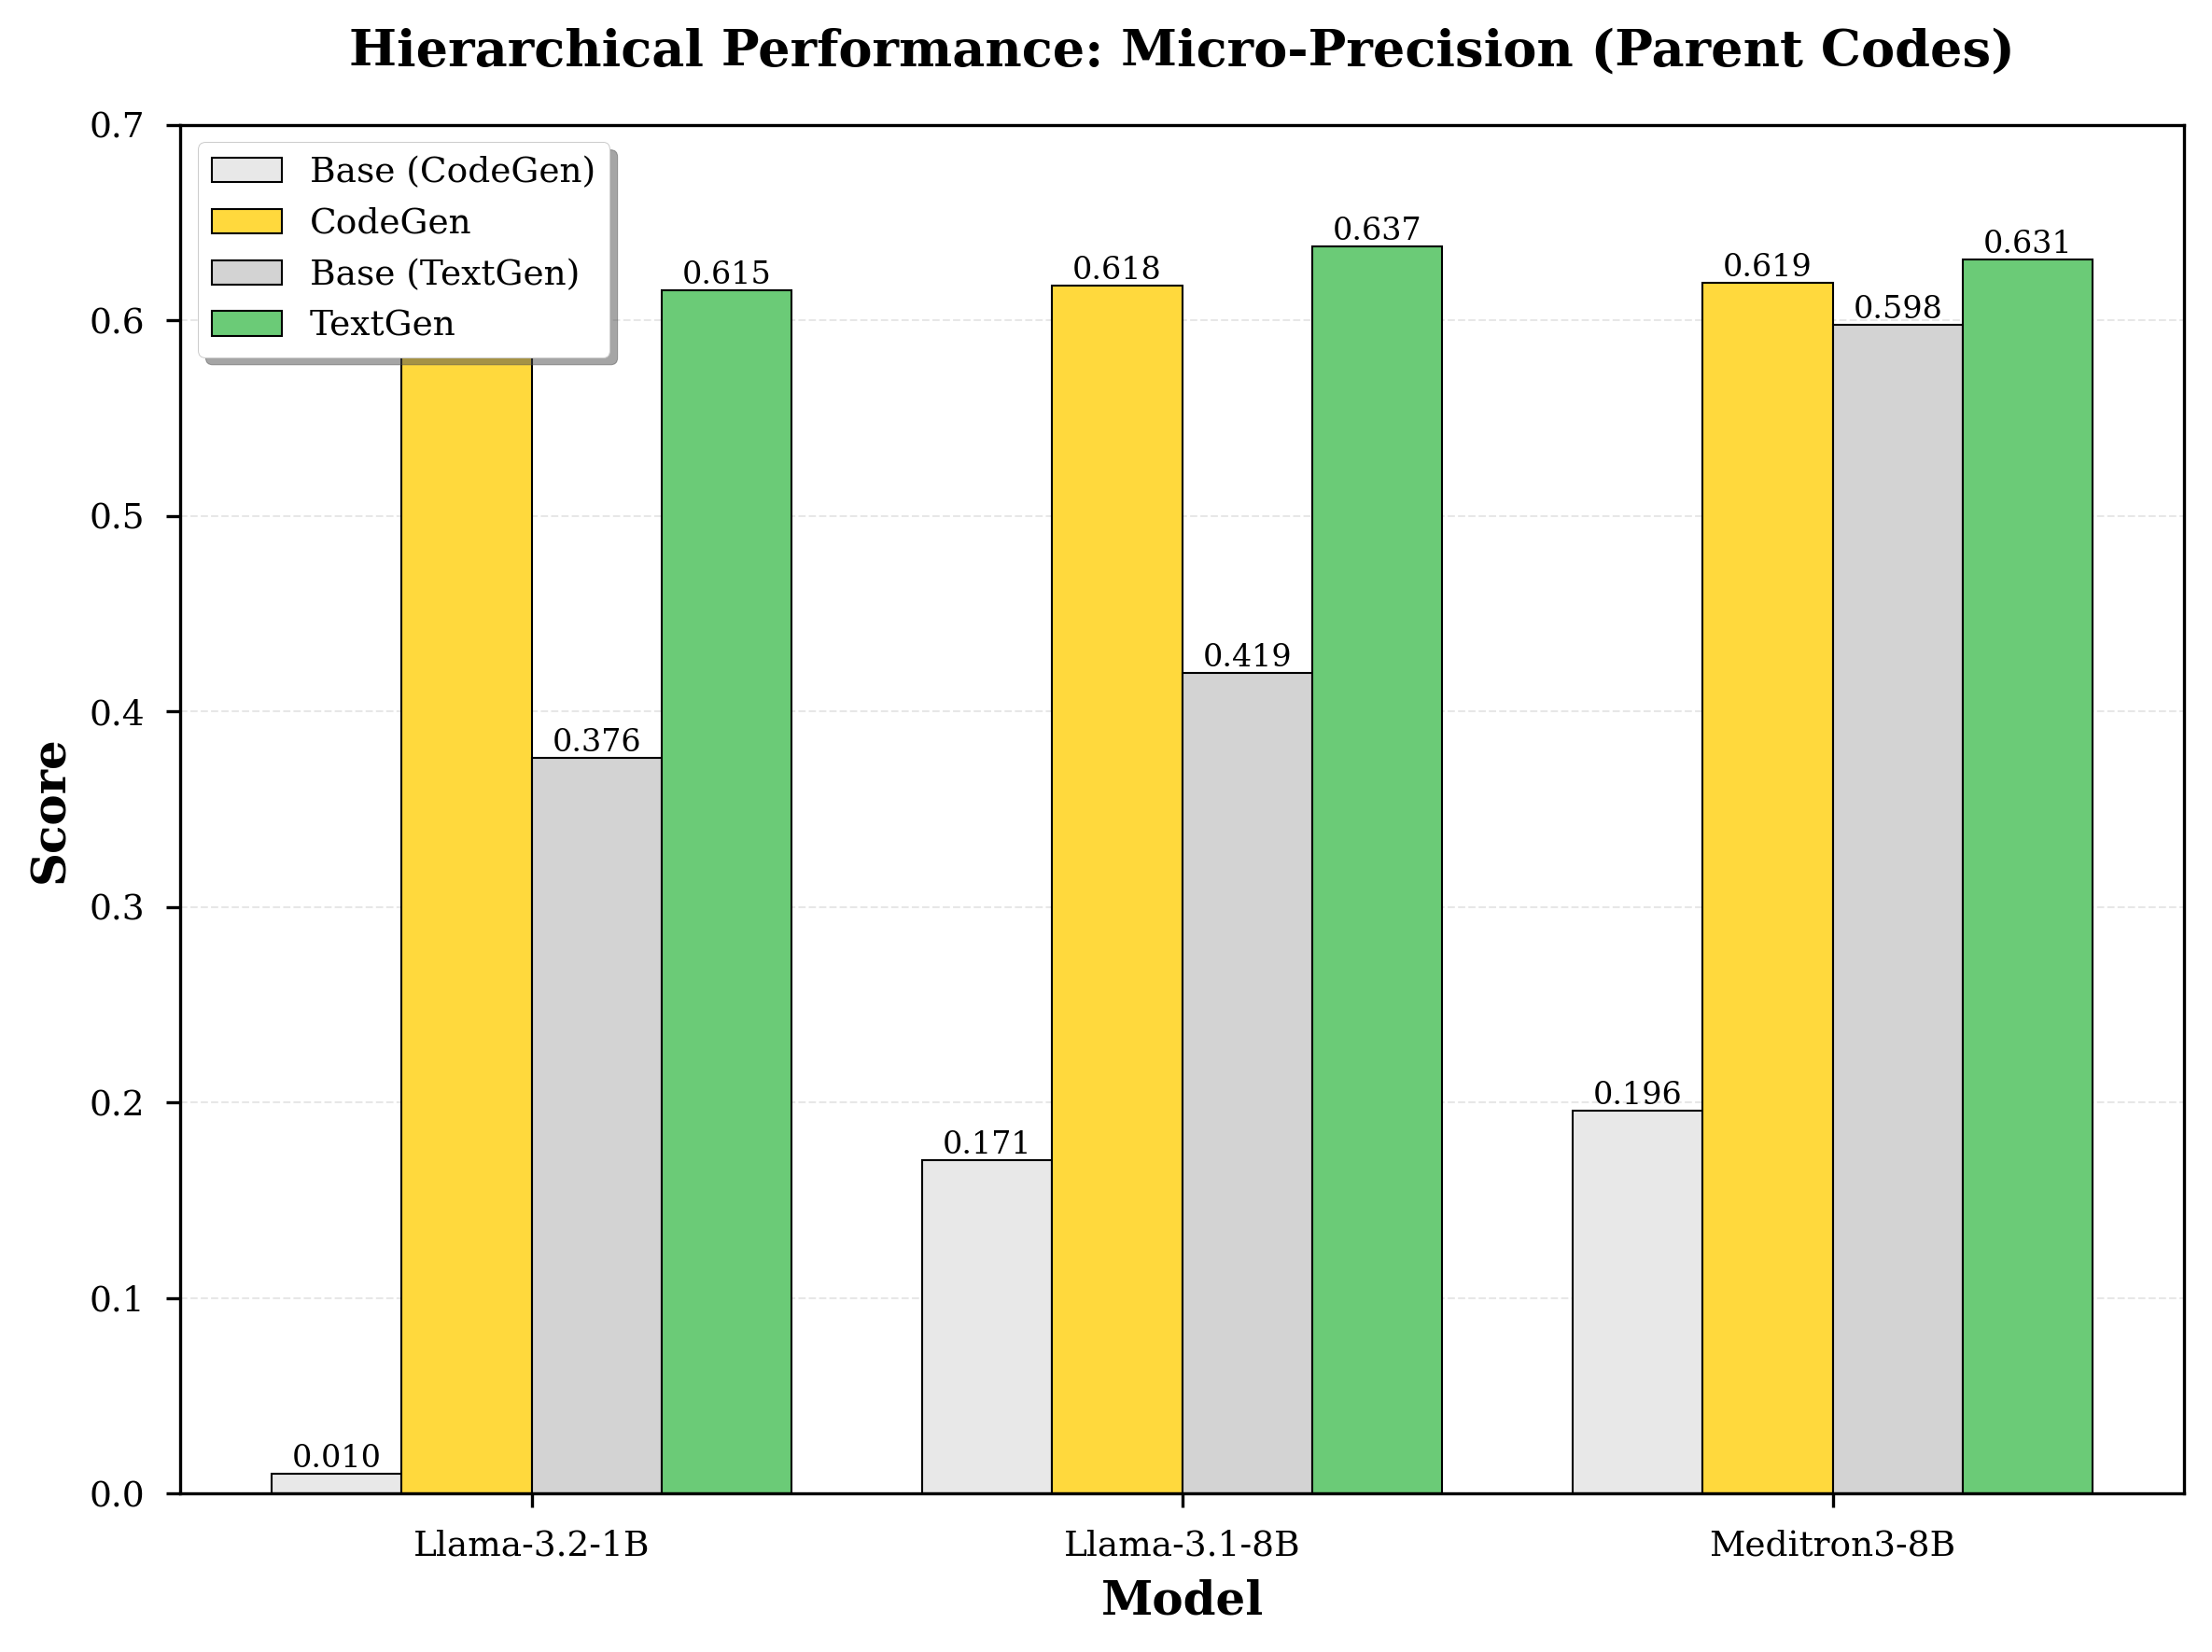
\includegraphics[width=\linewidth]{Images/Plots_thesis/parent_micro_precision.png}
        \caption{Parent micro-Precision}
        \label{fig:task1-parent-microP}
    \end{subfigure}\hfill
    \begin{subfigure}{0.32\textwidth}
        \centering
        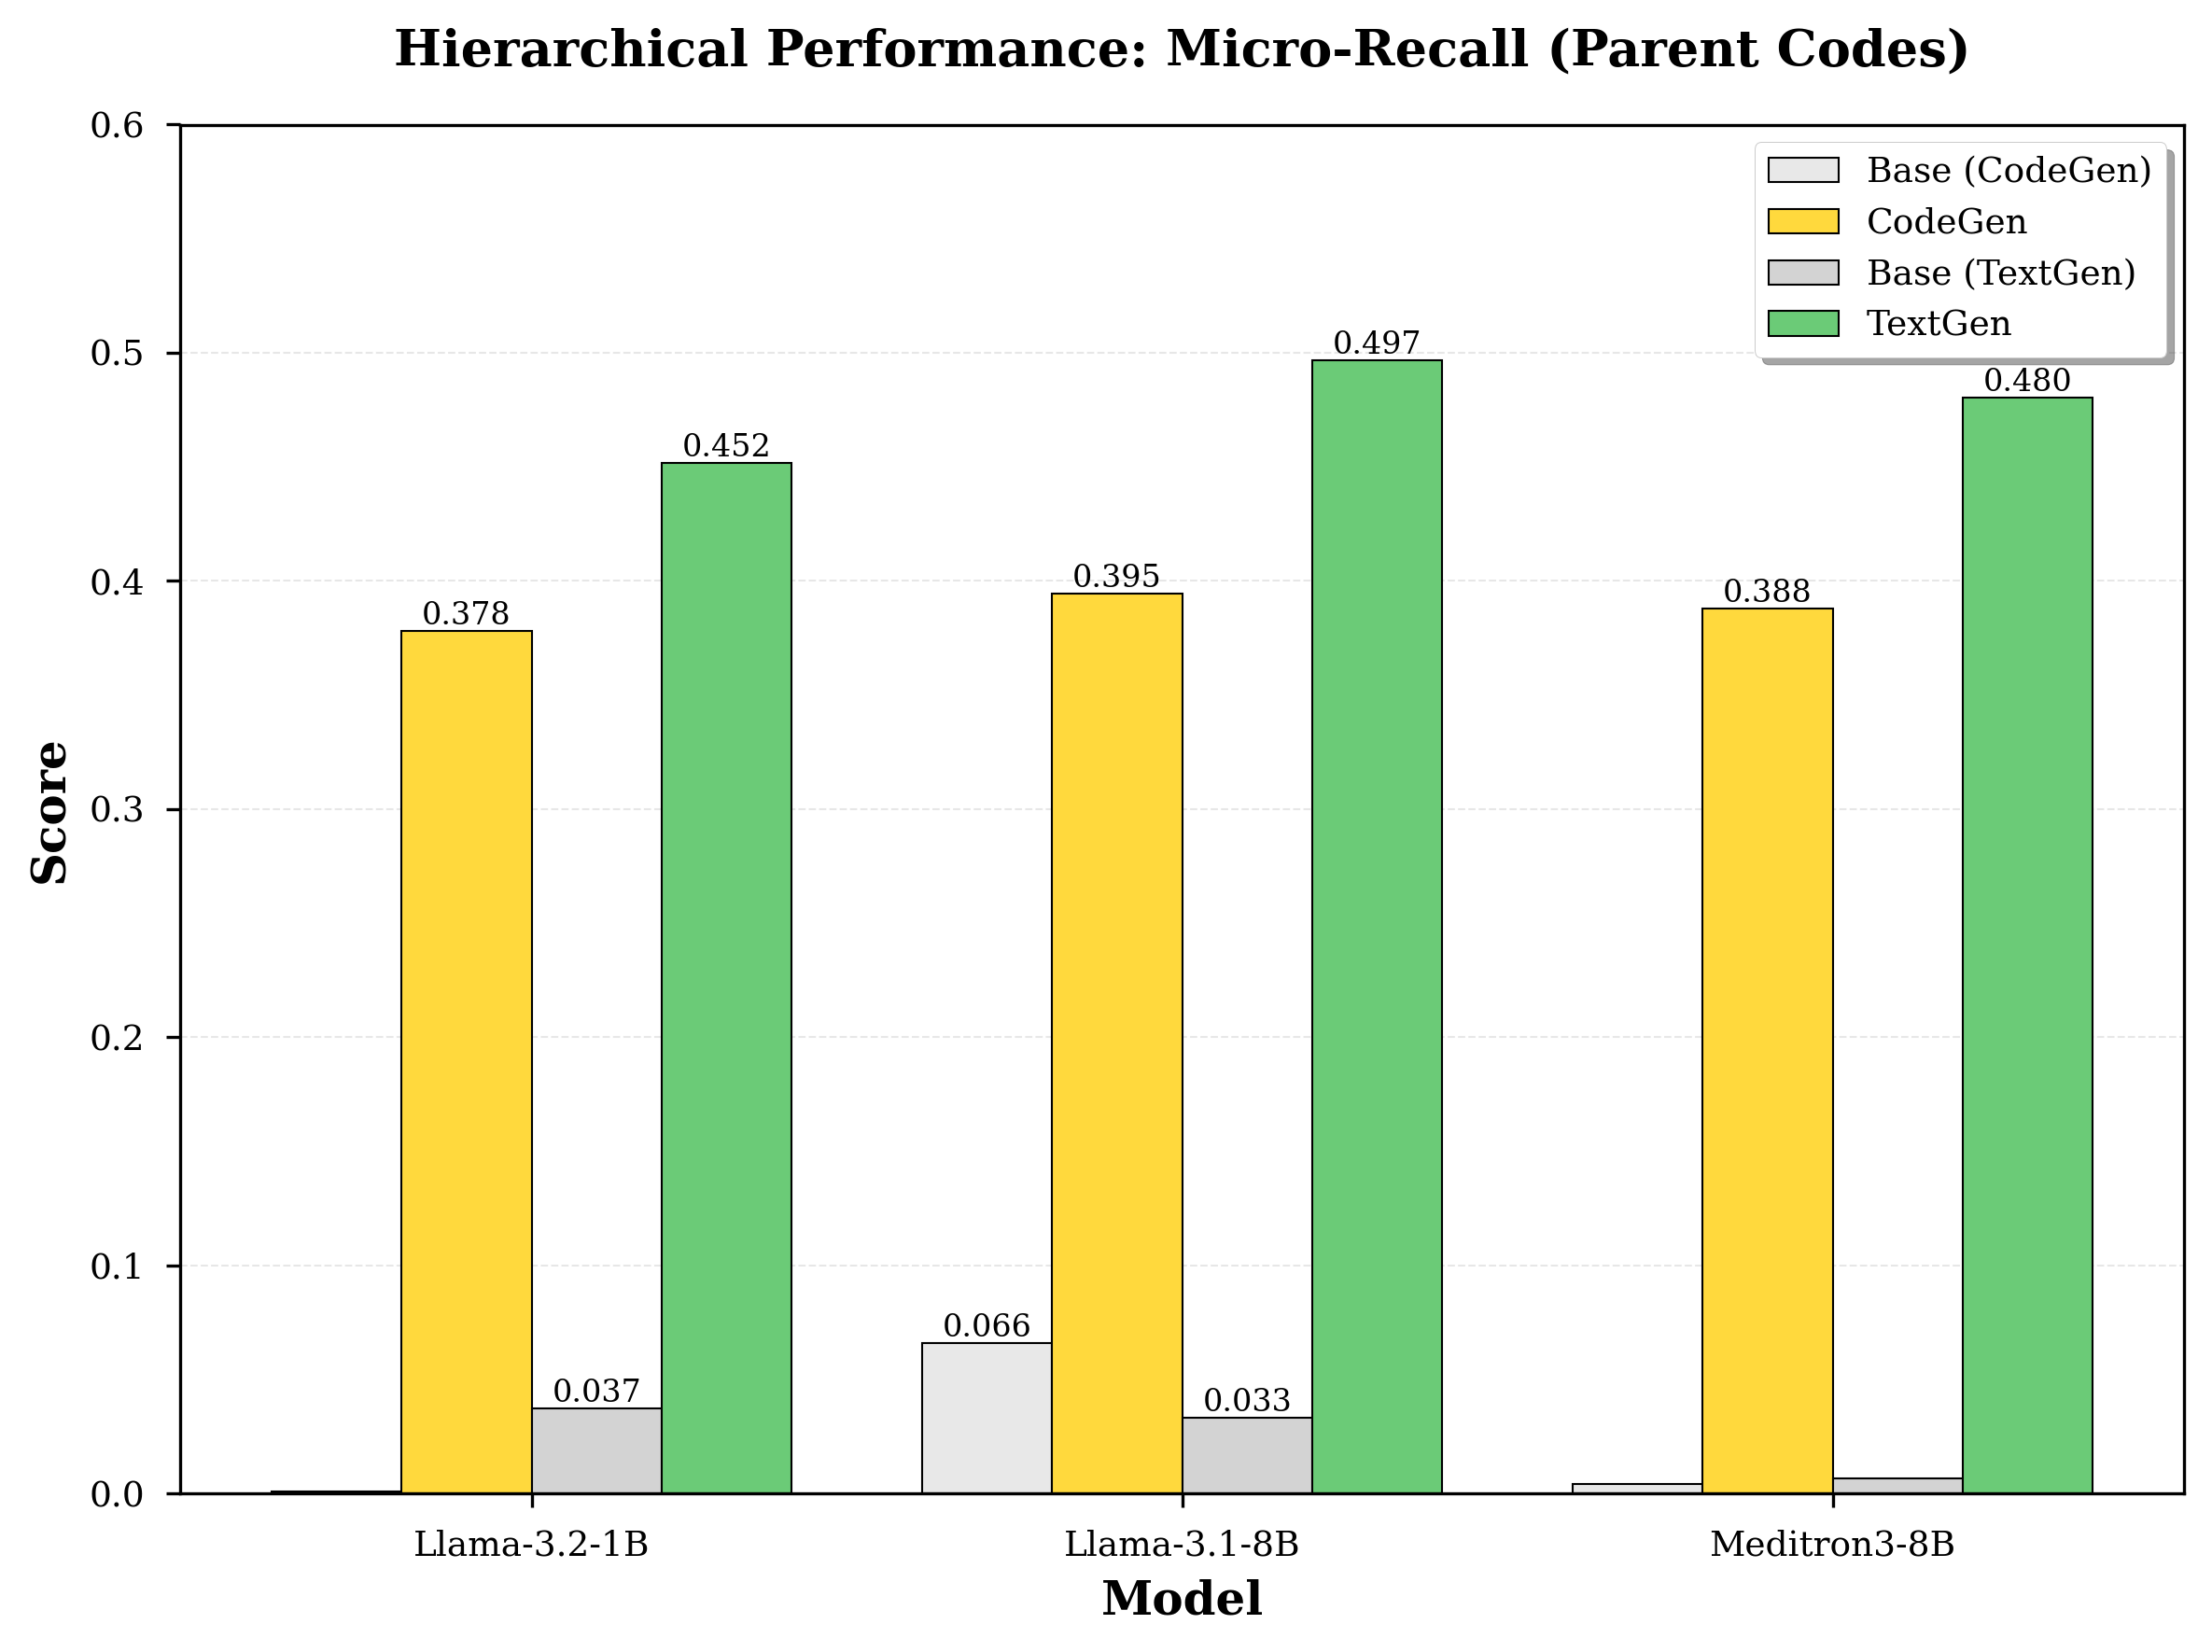
\includegraphics[width=\linewidth]{Images/Plots_thesis/parent_micro_recall.png}
        \caption{Parent micro-Recall}
        \label{fig:task1-parent-microR}
    \end{subfigure}\hfill
    \begin{subfigure}{0.32\textwidth}
        \centering
        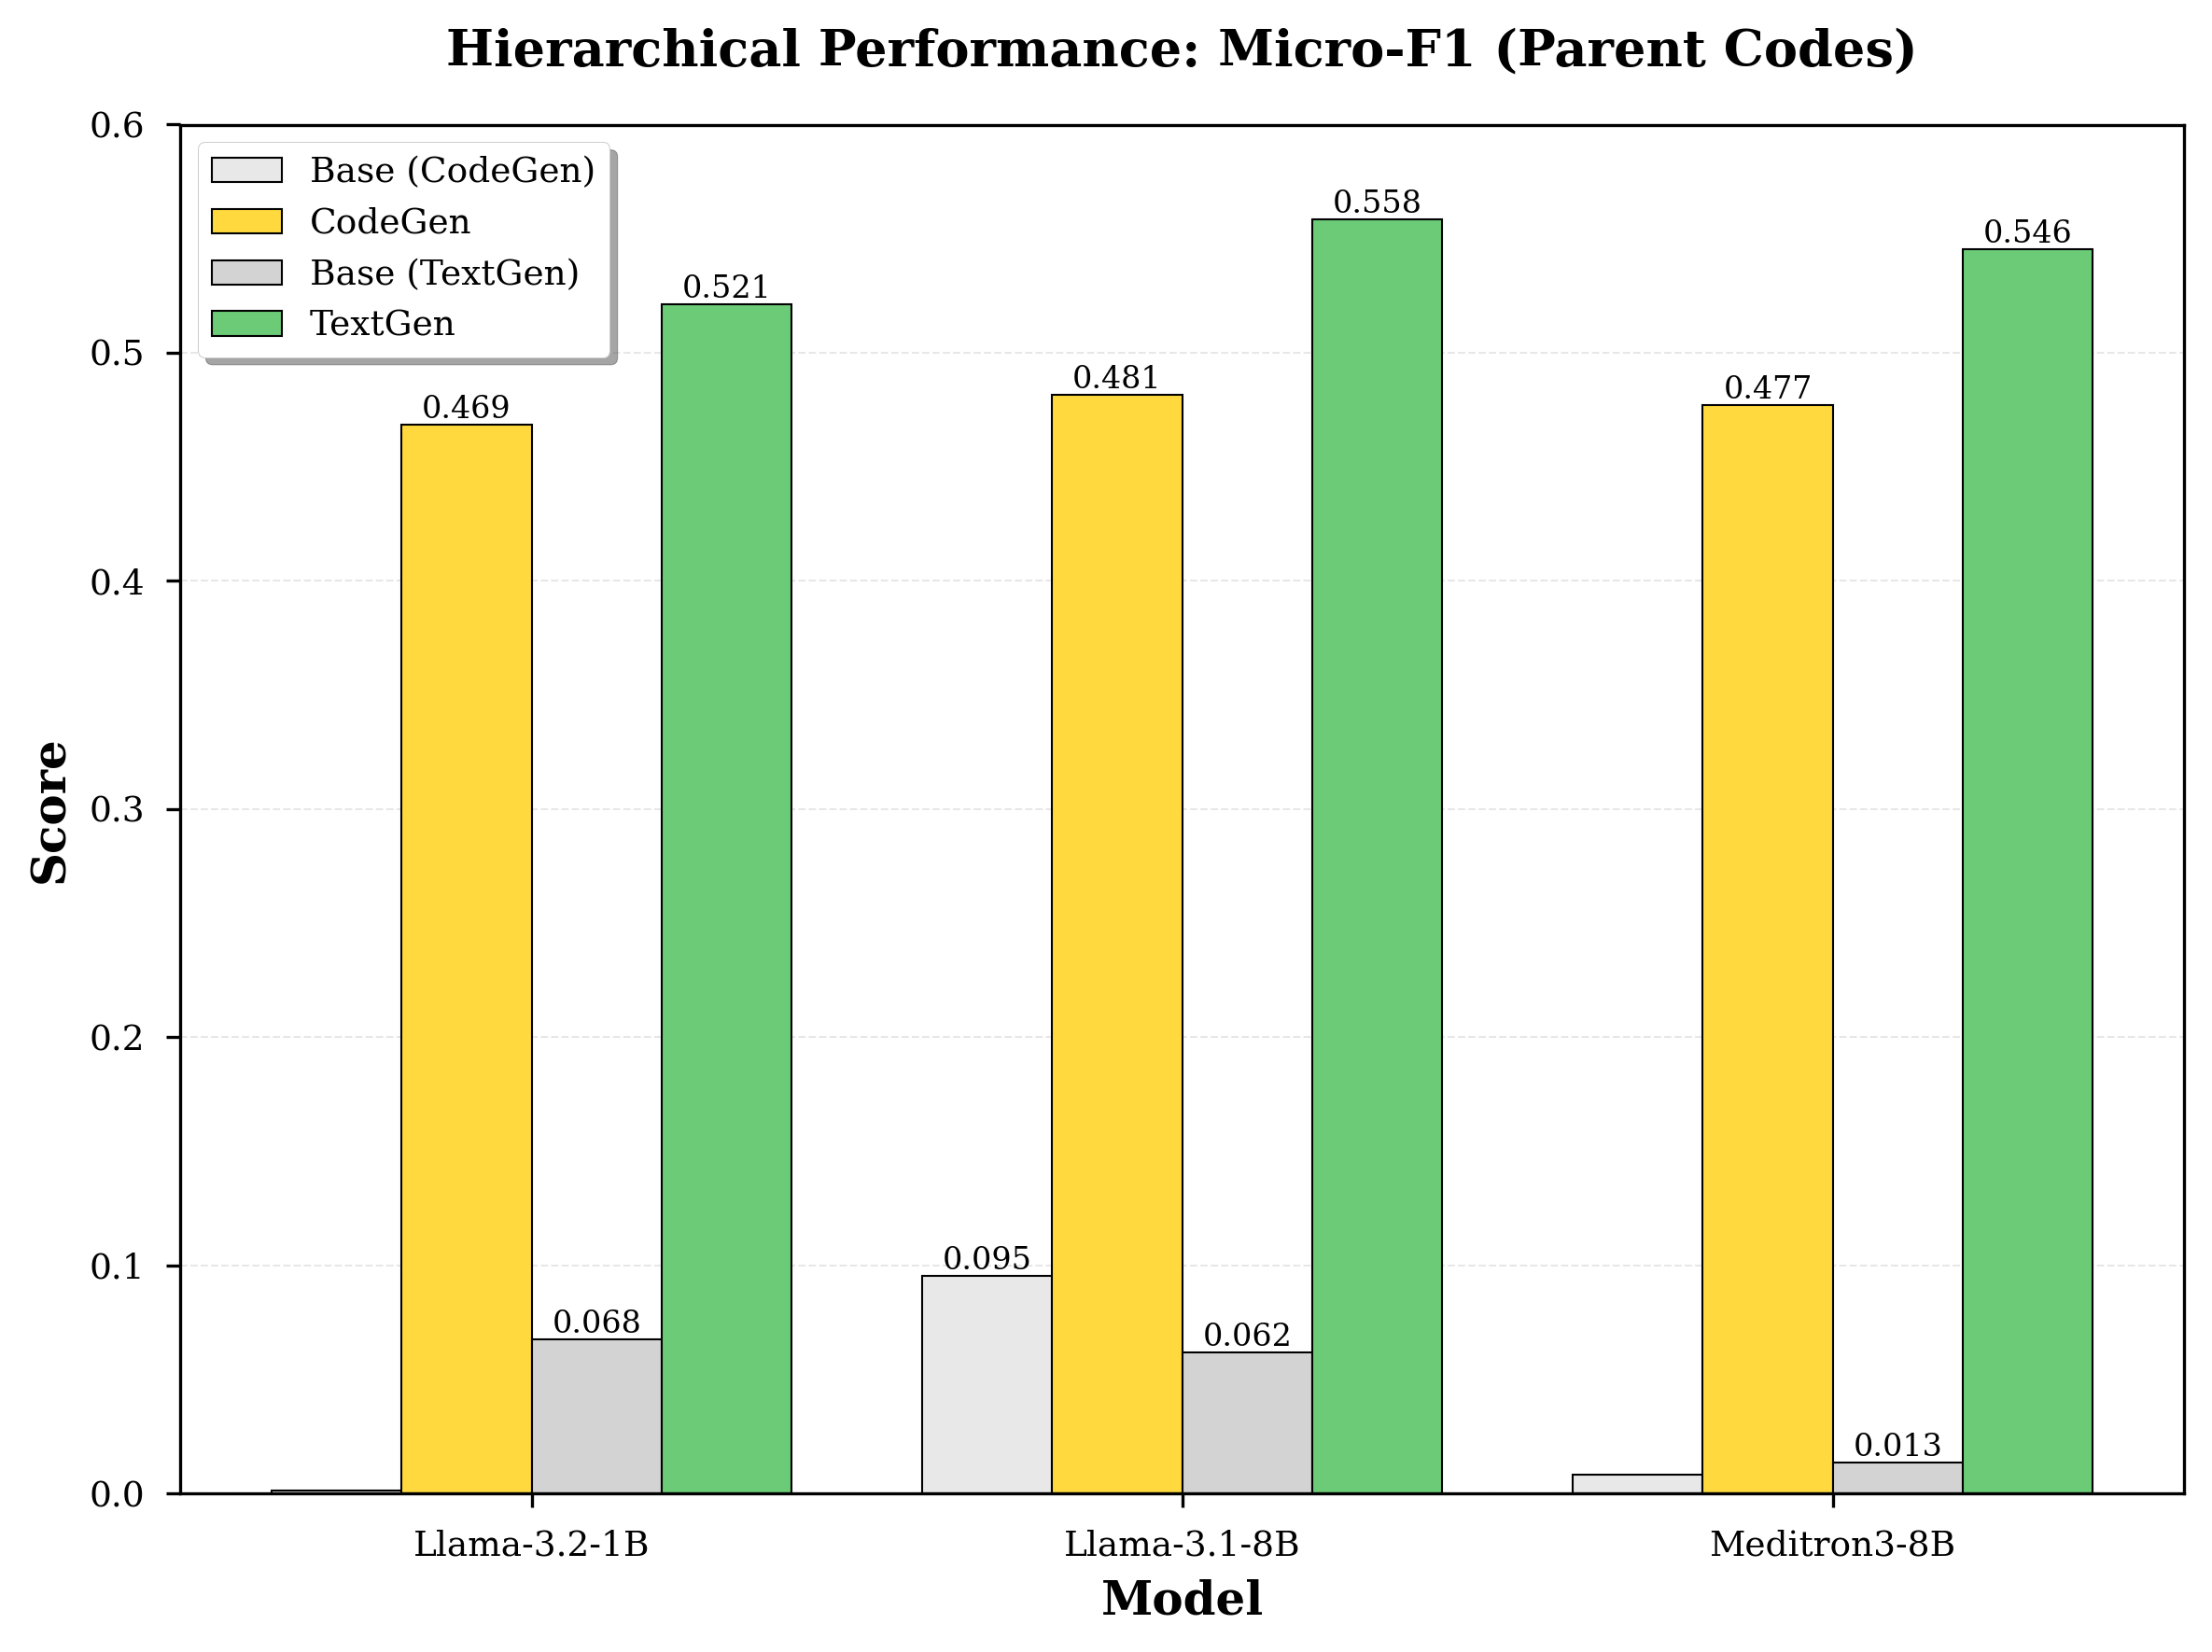
\includegraphics[width=\linewidth]{Images/Plots_thesis/parent_micro_f1.png}
        \caption{Parent micro-F1}
        \label{fig:task1-parent-microF1}
    \end{subfigure}

    \vspace{0.3cm}

    % Bottom row: macro-averaged parent metrics
    \begin{subfigure}{0.32\textwidth}
        \centering
        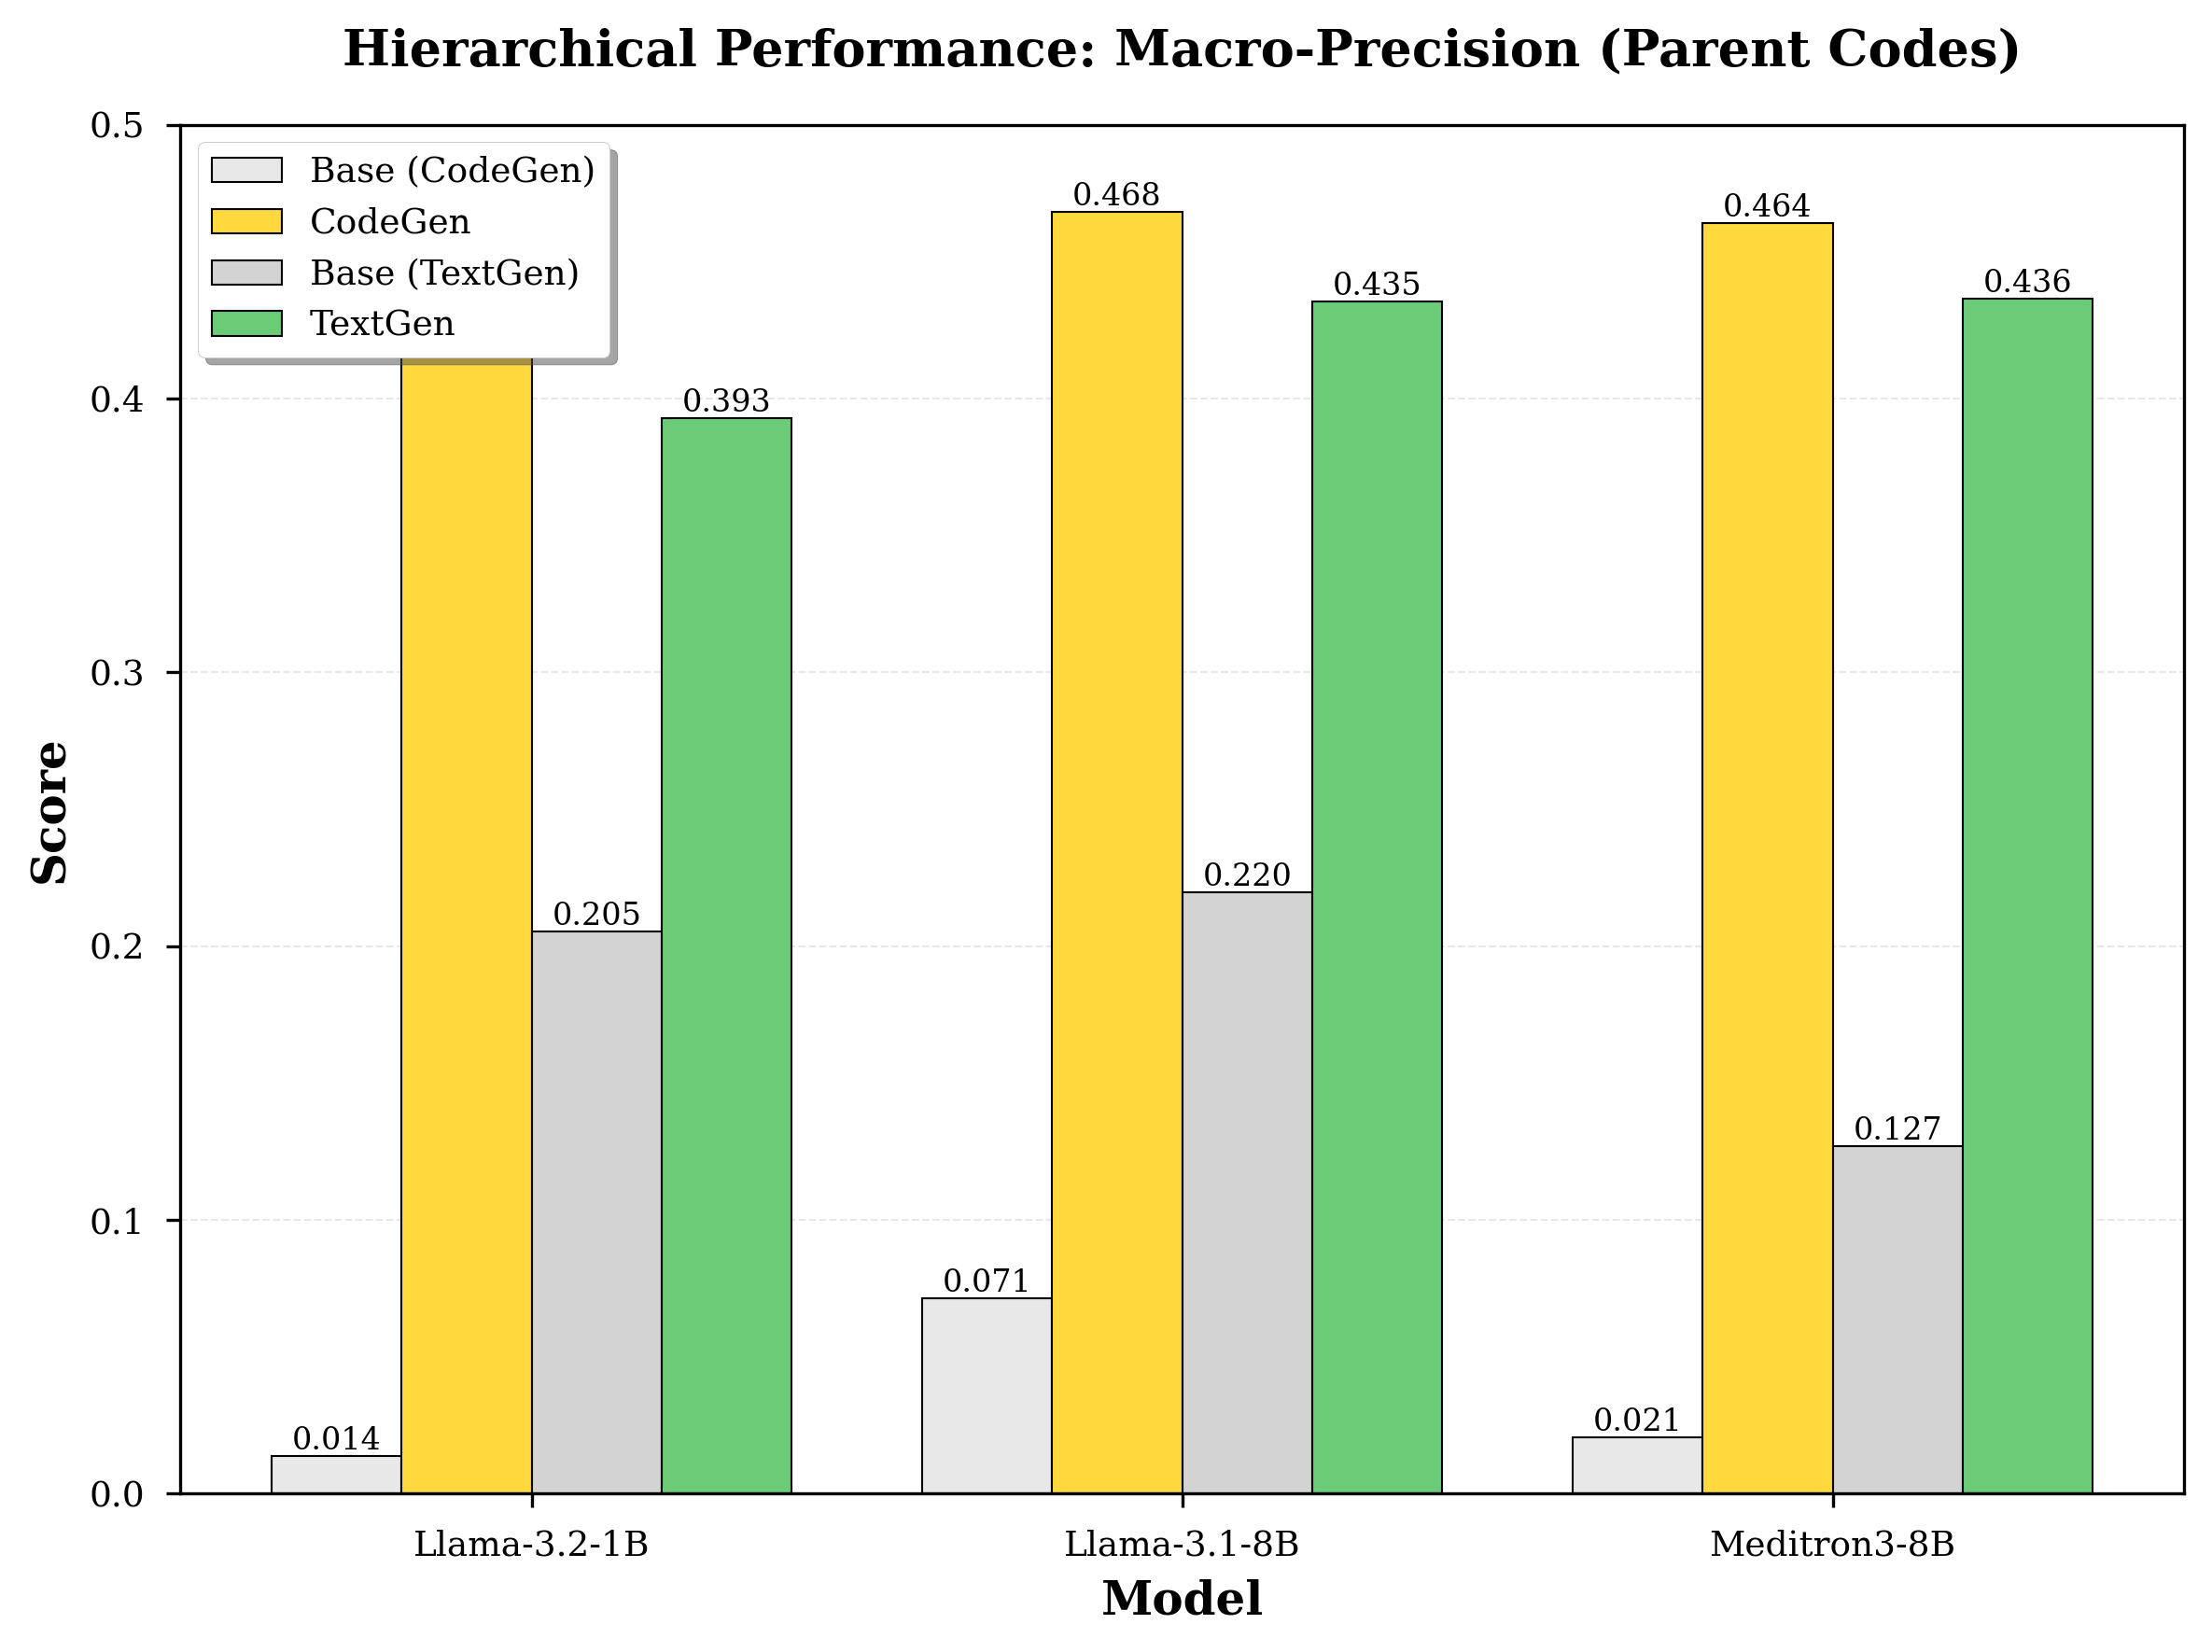
\includegraphics[width=\linewidth]{Images/Plots_thesis/parent_macro_precision.png}
        \caption{Parent macro-Precision}
        \label{fig:task1-parent-macroP}
    \end{subfigure}\hfill
    \begin{subfigure}{0.32\textwidth}
        \centering
        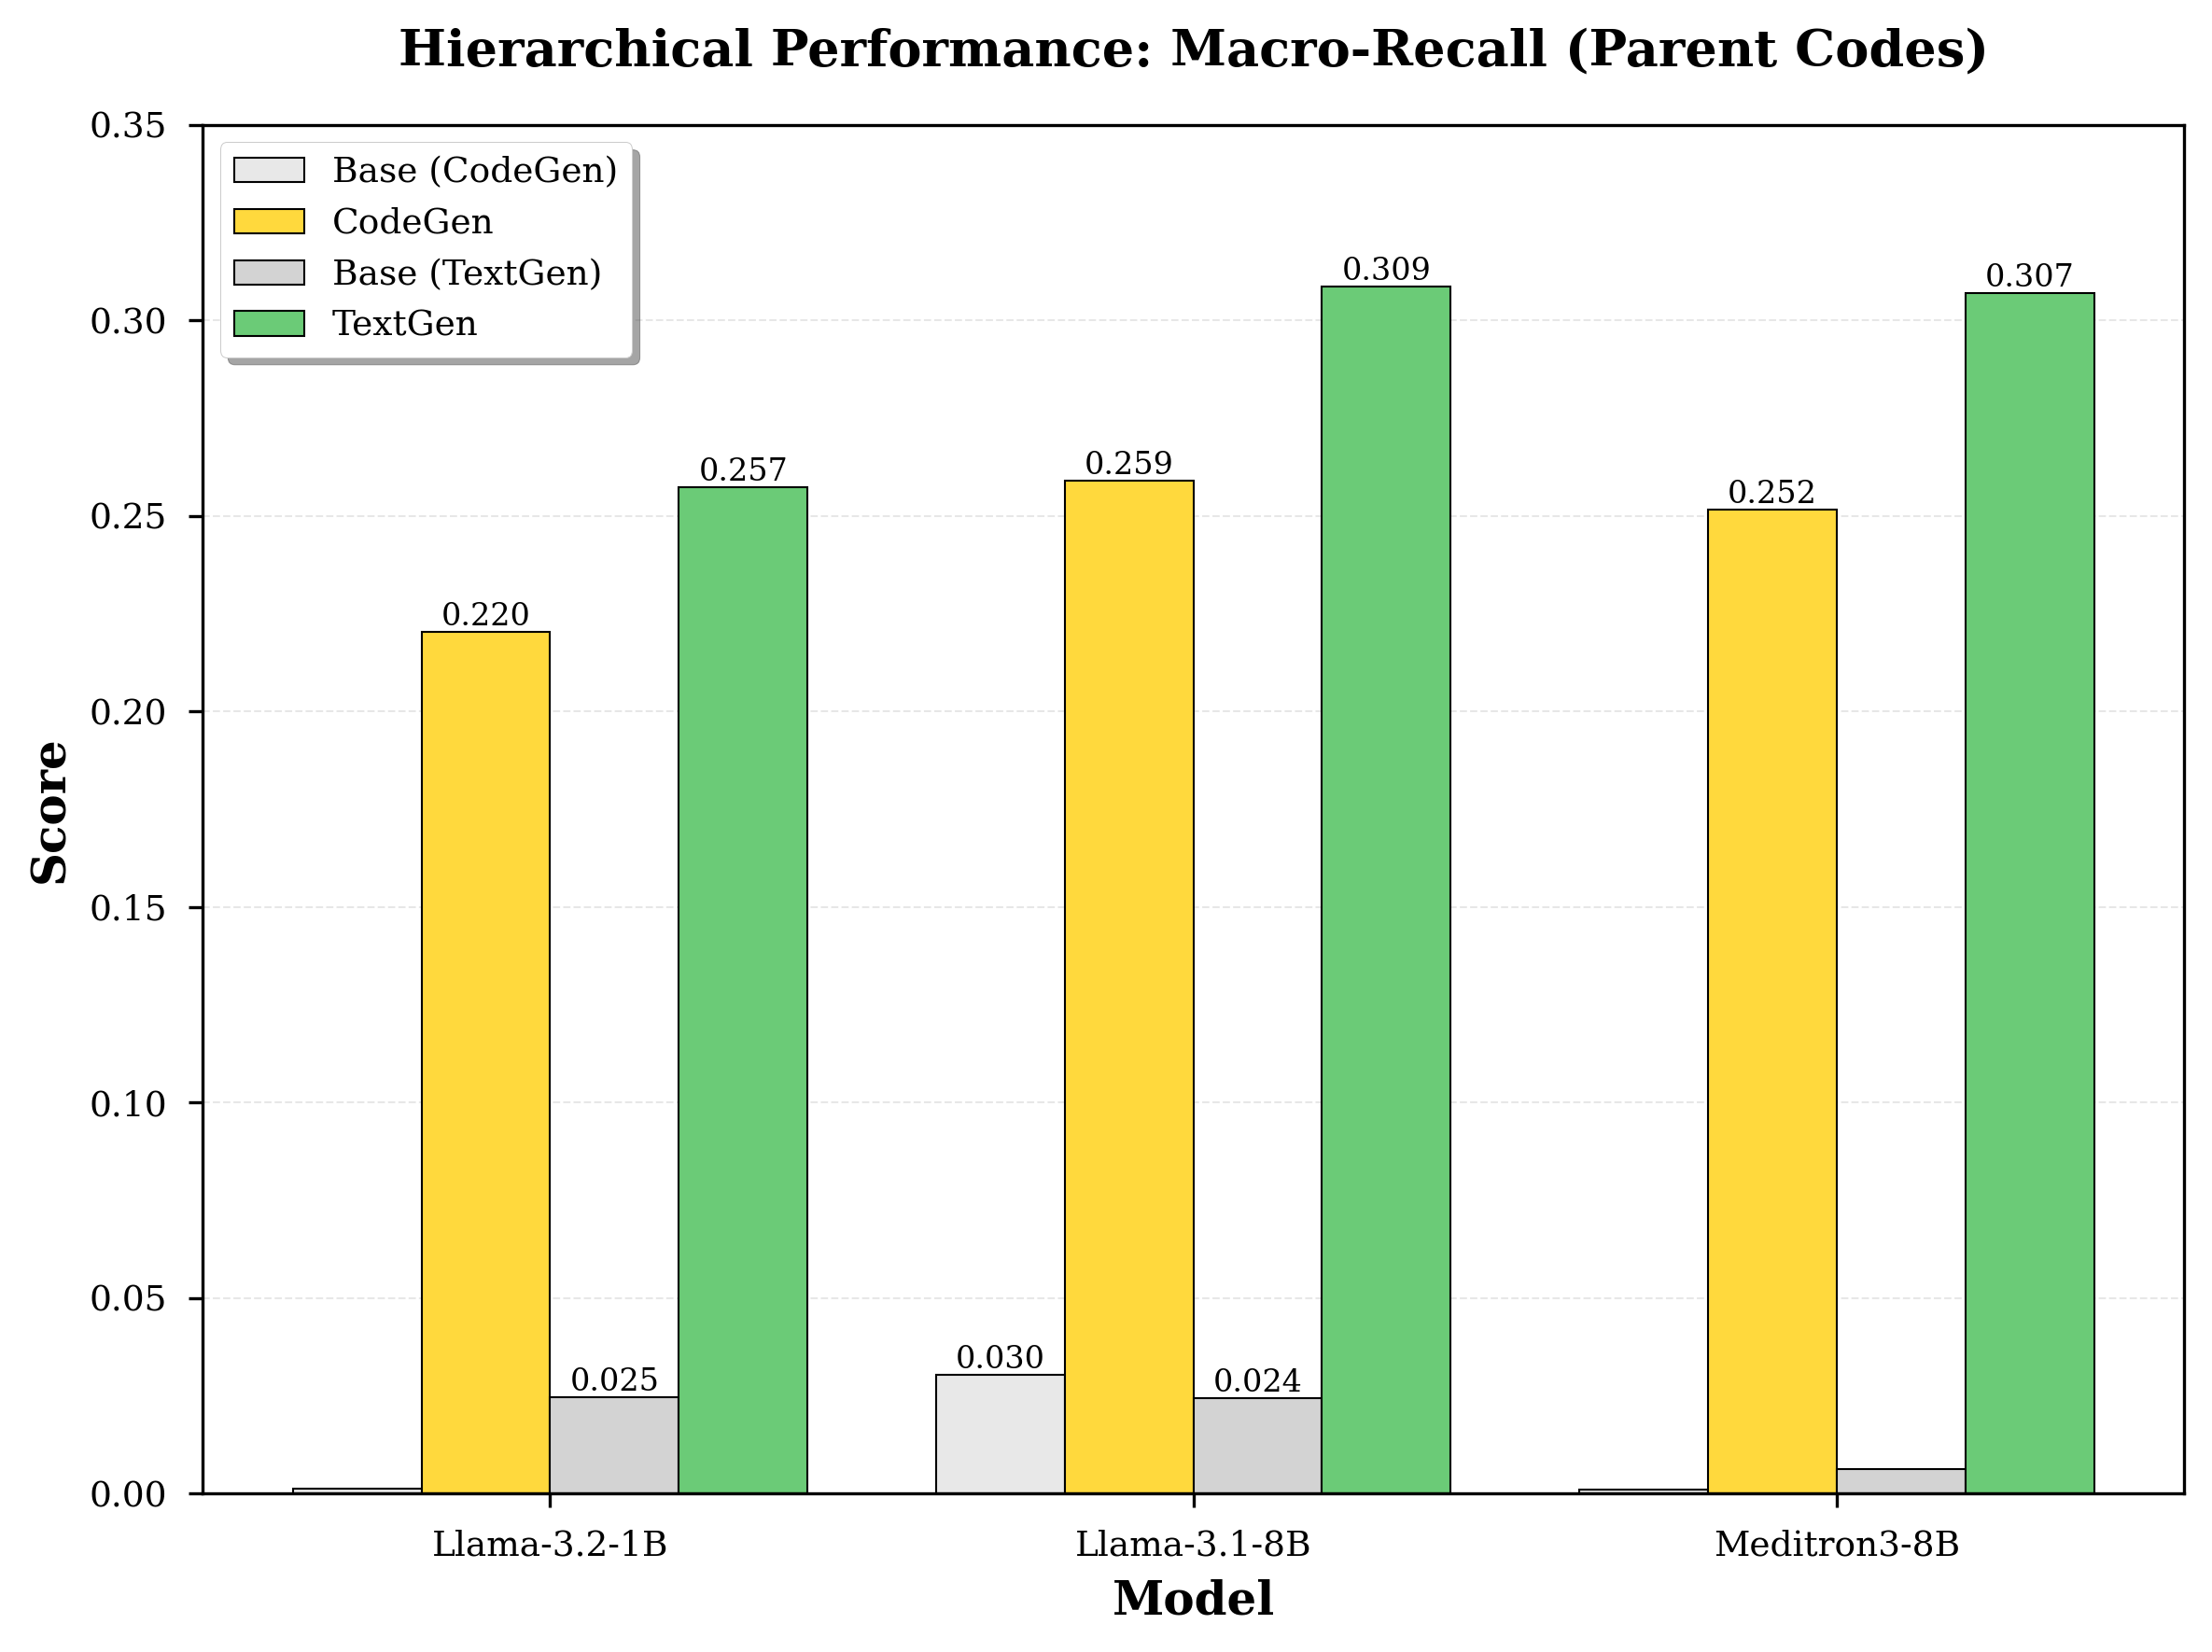
\includegraphics[width=\linewidth]{Images/Plots_thesis/parent_macro_recall.png}
        \caption{Parent macro-Recall}
        \label{fig:task1-parent-macroR}
    \end{subfigure}\hfill
    \begin{subfigure}{0.32\textwidth}
        \centering
        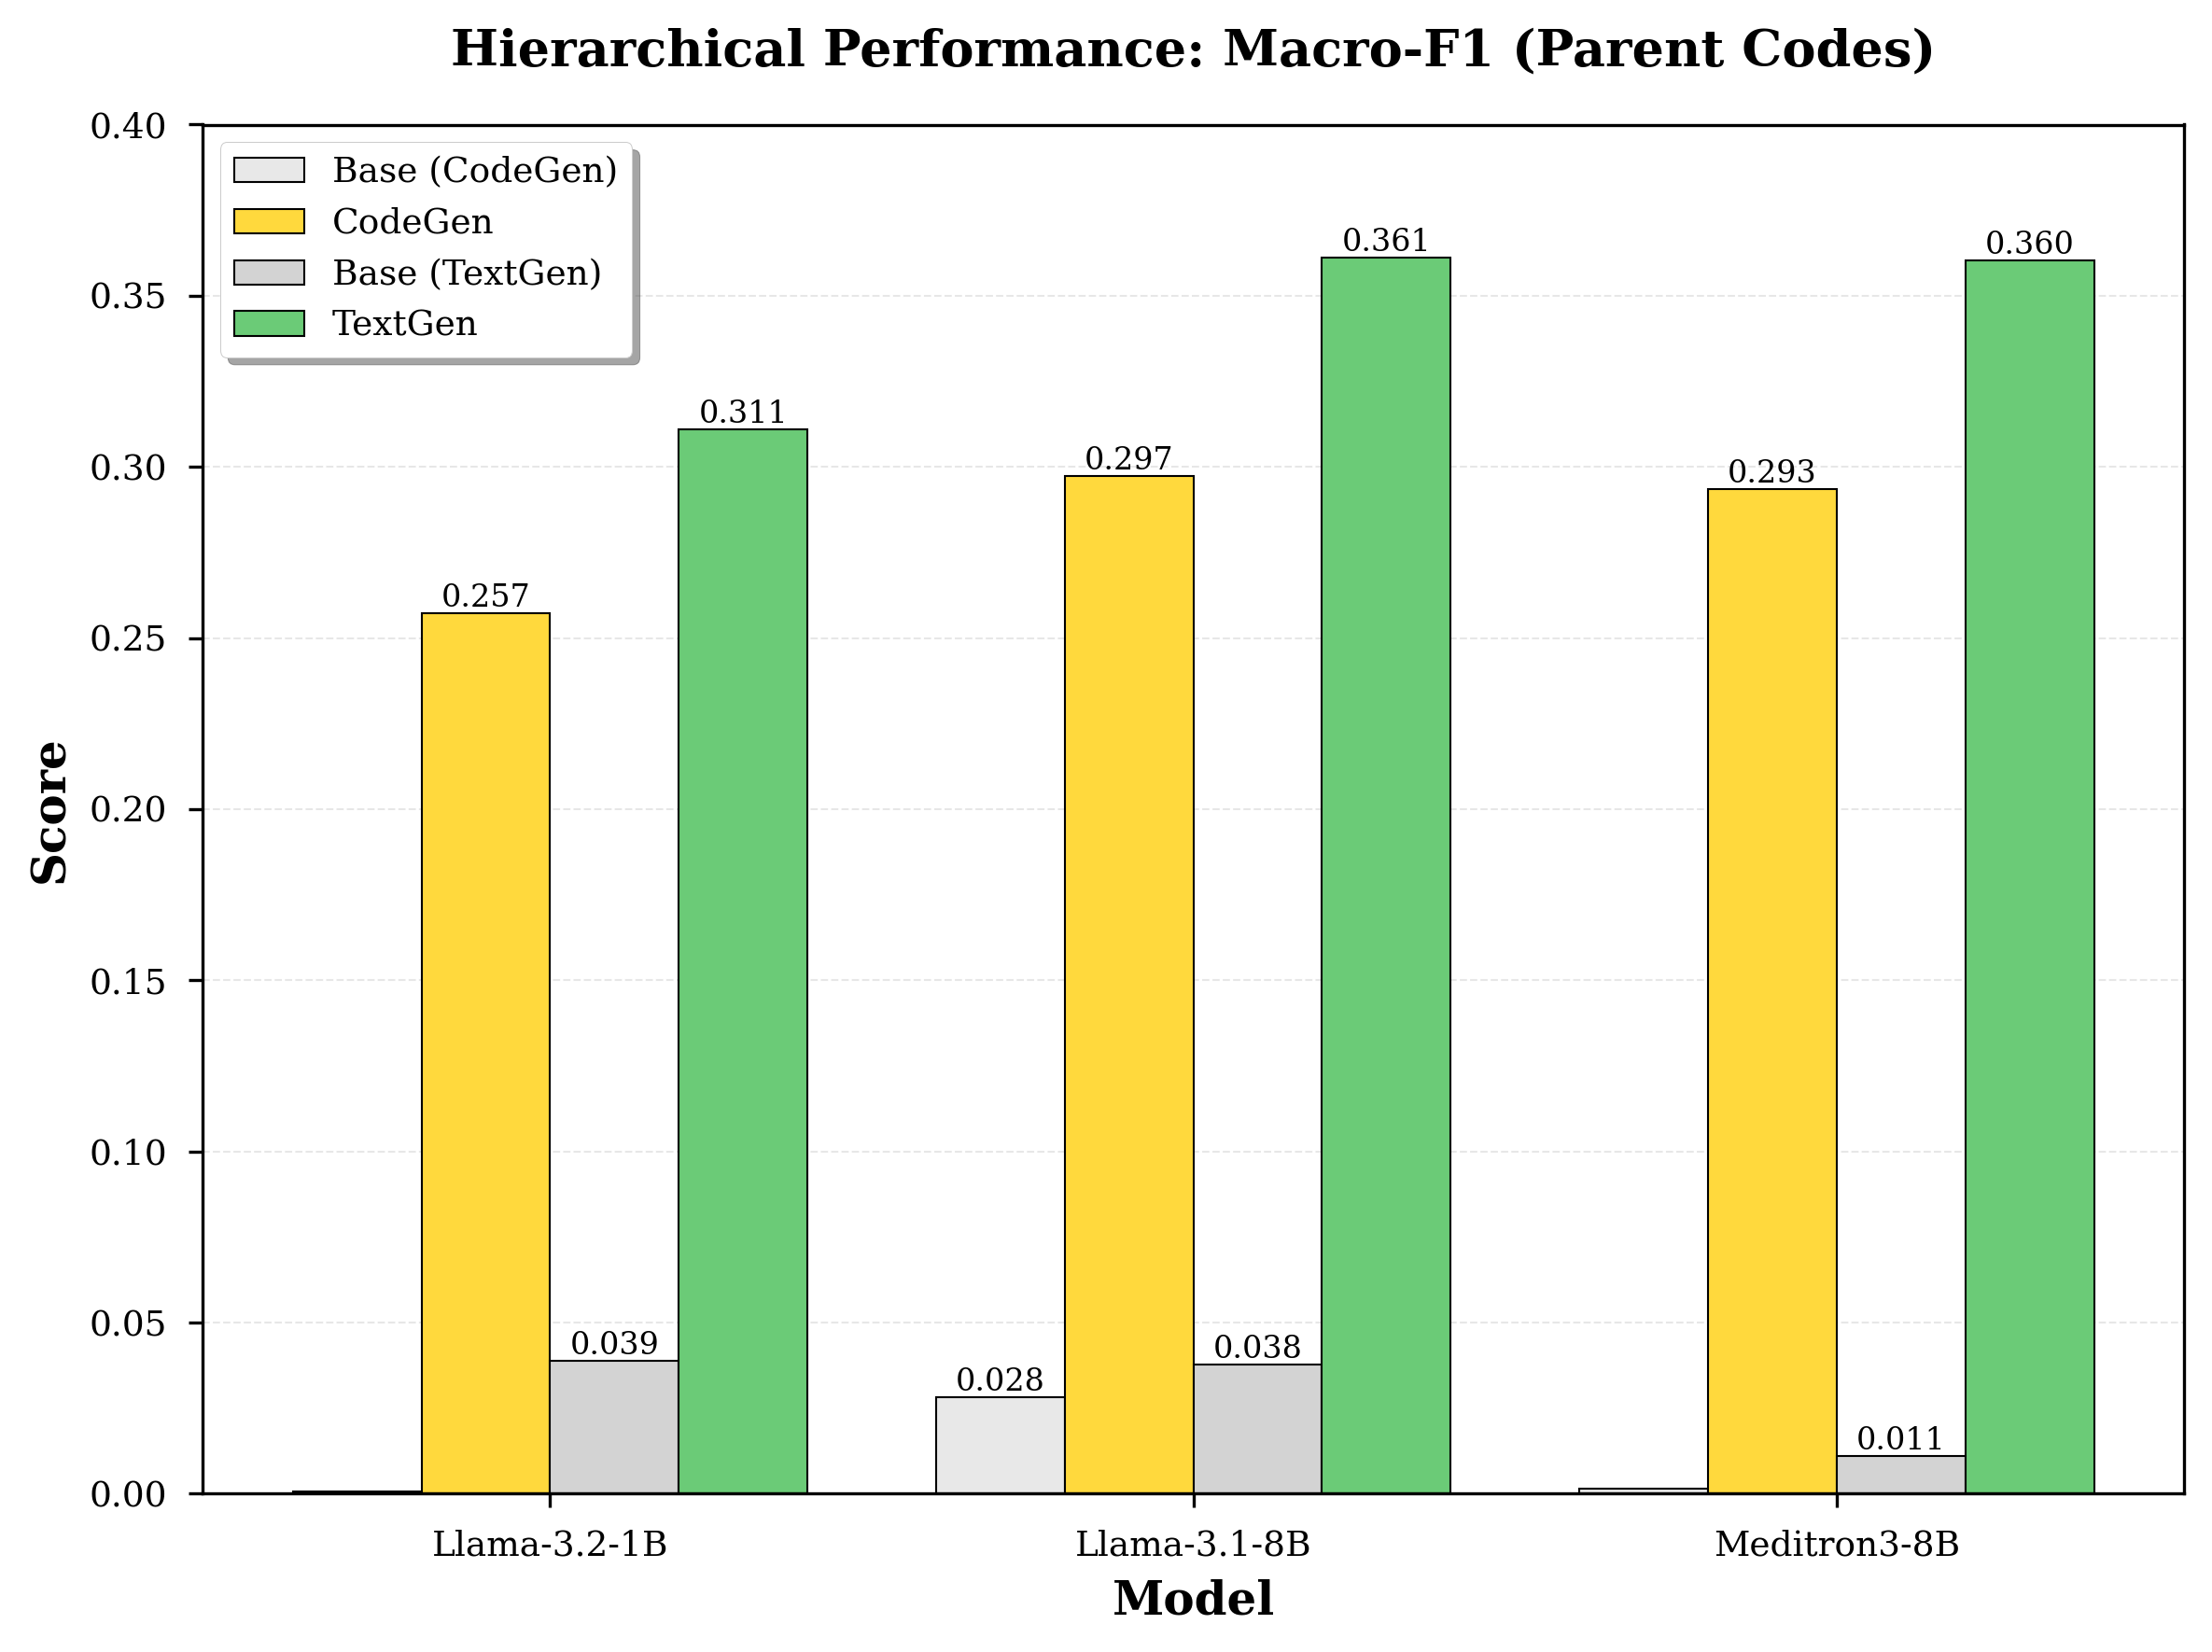
\includegraphics[width=\linewidth]{Images/Plots_thesis/parent_macro_f1.png}
        \caption{Parent macro-F1}
        \label{fig:task1-parent-macroF1}
    \end{subfigure}

    \caption{Task~1 hierarchical evaluation: parent-level micro/macro precision, recall, and F1 for \textbf{Base}, \textbf{CodeGen}, and \textbf{TextGen} across backbones. Parent evaluation reveals clinically meaningful ``near misses'' at the full-code level.}
    \label{fig:task1-parent-metrics}
\end{figure}

% ============================================================
\subsection{Head--Tail Behaviour: Performance on Frequent vs.\ Rare Codes}
\label{subsec:results-task1-headtail}

Overall micro-averaged metrics are dominated by frequent codes, while macro-averaged metrics are sensitive to poor tail performance. To explicitly characterise label imbalance, we evaluate models on two extremal subsets of the label space: the \textbf{Top-50} (Head-50) and \textbf{Bottom-50} (Tail-50) ICD-9 codes, defined by global code frequency across all splits (Section~\ref{subsec:head-tail-cohort}). 

\paragraph{Top-50 codes (Head-50).}
Table~\ref{tab:task1-top50} shows that TextGen achieves strong performance on frequent diagnoses across all backbones and substantially exceeds CodeGen. This indicates that when sufficient supervised signal exists, TextGen can use its limited output budget effectively to prioritise prevalent diagnoses.

\begin{table}[t]
\centering
\caption{Task~1 performance restricted to the Top-50 most frequent ICD-9 codes (Head-50) on the test set.}
\label{tab:task1-top50}
\begin{tabular}{llcc}
\toprule
\textbf{Backbone} & \textbf{Method} & \textbf{Micro-F1} & \textbf{Macro-F1} \\
\midrule
\multirow{4}{*}{Llama-3.2-1B}
& Base (CodeGen) & 0.0002 & 0.0001 \\
& CodeGen        & 0.3292 & 0.2670 \\
& Base (TextGen) & 0.0496 & 0.0351 \\
& TextGen        & \textbf{0.5329} & \textbf{0.4846} \\
\midrule
\multirow{4}{*}{Llama-3.1-8B}
& Base (CodeGen) & 0.0646 & 0.0315 \\
& CodeGen        & 0.3413 & 0.2784 \\
& Base (TextGen) & 0.0439 & 0.0300 \\
& TextGen        & \textbf{0.5876} & \textbf{0.5347} \\
\midrule
\multirow{4}{*}{Meditron-8B}
& Base (CodeGen) & 0.0101 & 0.0054 \\
& CodeGen        & 0.3342 & 0.2723 \\
& Base (TextGen) & 0.0030 & 0.0028 \\
& TextGen        & \textbf{0.5845} & \textbf{0.5253} \\
\bottomrule
\end{tabular}
\end{table}

\paragraph{Bottom-50 codes (Tail-50).}
Table~\ref{tab:task1-bottom50} reveals sharp degradation on rare diagnoses. Tail-50 values can be extremely small because each rare code has low support in the test set; even a small number of additional correct predictions can change tail micro/macro metrics substantially. Notably, with the updated baselines, TextGen achieves non-zero Tail-50 performance across all backbones, making tail improvements under KG augmentation a strict and meaningful comparison rather than an artifact of lifting a degenerate zero baseline.

\begin{table}[t]
\centering
\caption{Task~1 performance restricted to the Bottom-50 rarest ICD-9 codes (Tail-50) on the test set.}
\label{tab:task1-bottom50}
\begin{tabular}{llcc}
\toprule
\textbf{Backbone} & \textbf{Method} & \textbf{Micro-F1} & \textbf{Macro-F1} \\
\midrule
\multirow{4}{*}{Llama-3.2-1B}
& Base (CodeGen) & 0.0000 & 0.0000 \\
& CodeGen        & 0.1304 & 0.0367 \\
& Base (TextGen) & 0.0000 & 0.0000 \\
& TextGen        & \textbf{0.1429} & \textbf{0.0655} \\
\midrule
\multirow{4}{*}{Llama-3.1-8B}
& Base (CodeGen) & 0.0129 & 0.0025 \\
& CodeGen        & 0.1200 & 0.0600 \\
& Base (TextGen) & 0.0488 & 0.0345 \\
& TextGen        & \textbf{0.1250} & \textbf{0.0713} \\
\midrule
\multirow{4}{*}{Meditron-8B}
& Base (CodeGen) & 0.0000 & 0.0000 \\
& CodeGen        & 0.1304 & 0.0133 \\
& Base (TextGen) & 0.0000 & 0.0000 \\
& TextGen        & \textbf{0.1518} & \textbf{0.0747} \\
\bottomrule
\end{tabular}
\end{table}

% --- UPDATED FIGURE BLOCK (as requested) ---
\begin{figure}[t]
    \centering
    % first row
    \begin{subfigure}{0.48\textwidth}
        \centering
        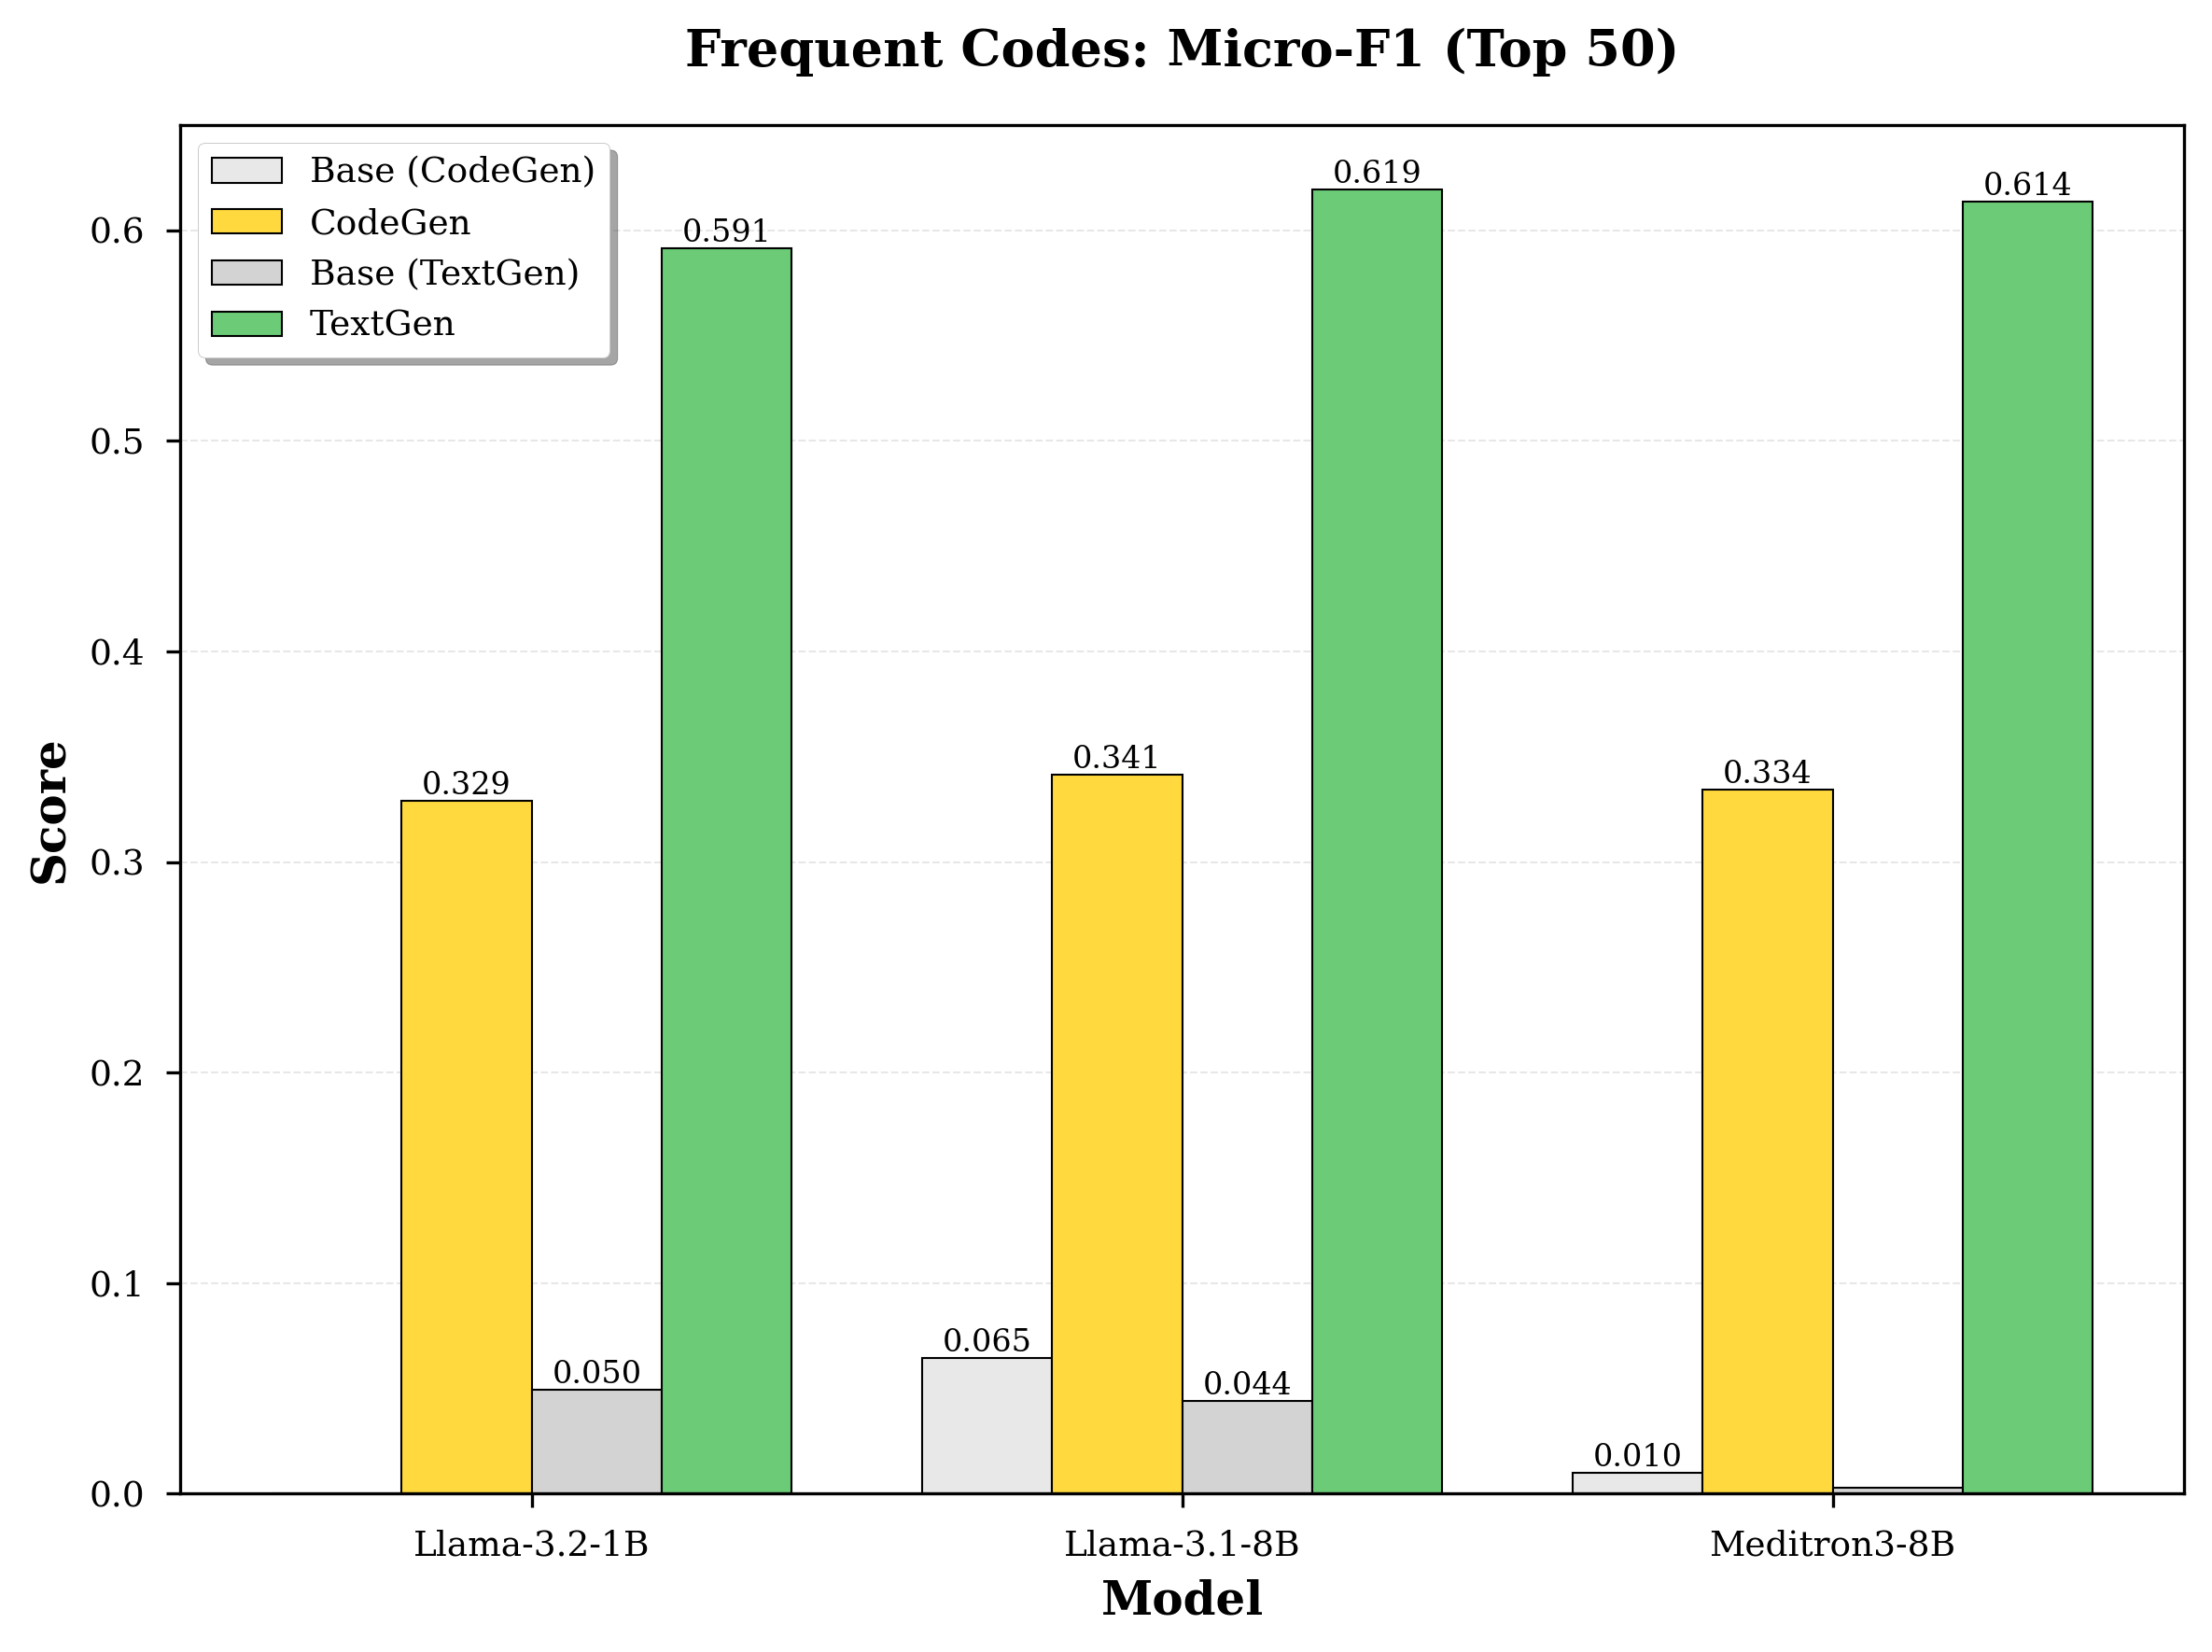
\includegraphics[width=\linewidth]{Images/Plots_thesis/top50_micro_f1.png}
        \caption{Top-50 micro-F1}
        \label{fig:task1-top50-microF1}
    \end{subfigure}\hfill
    \begin{subfigure}{0.48\textwidth}
        \centering
        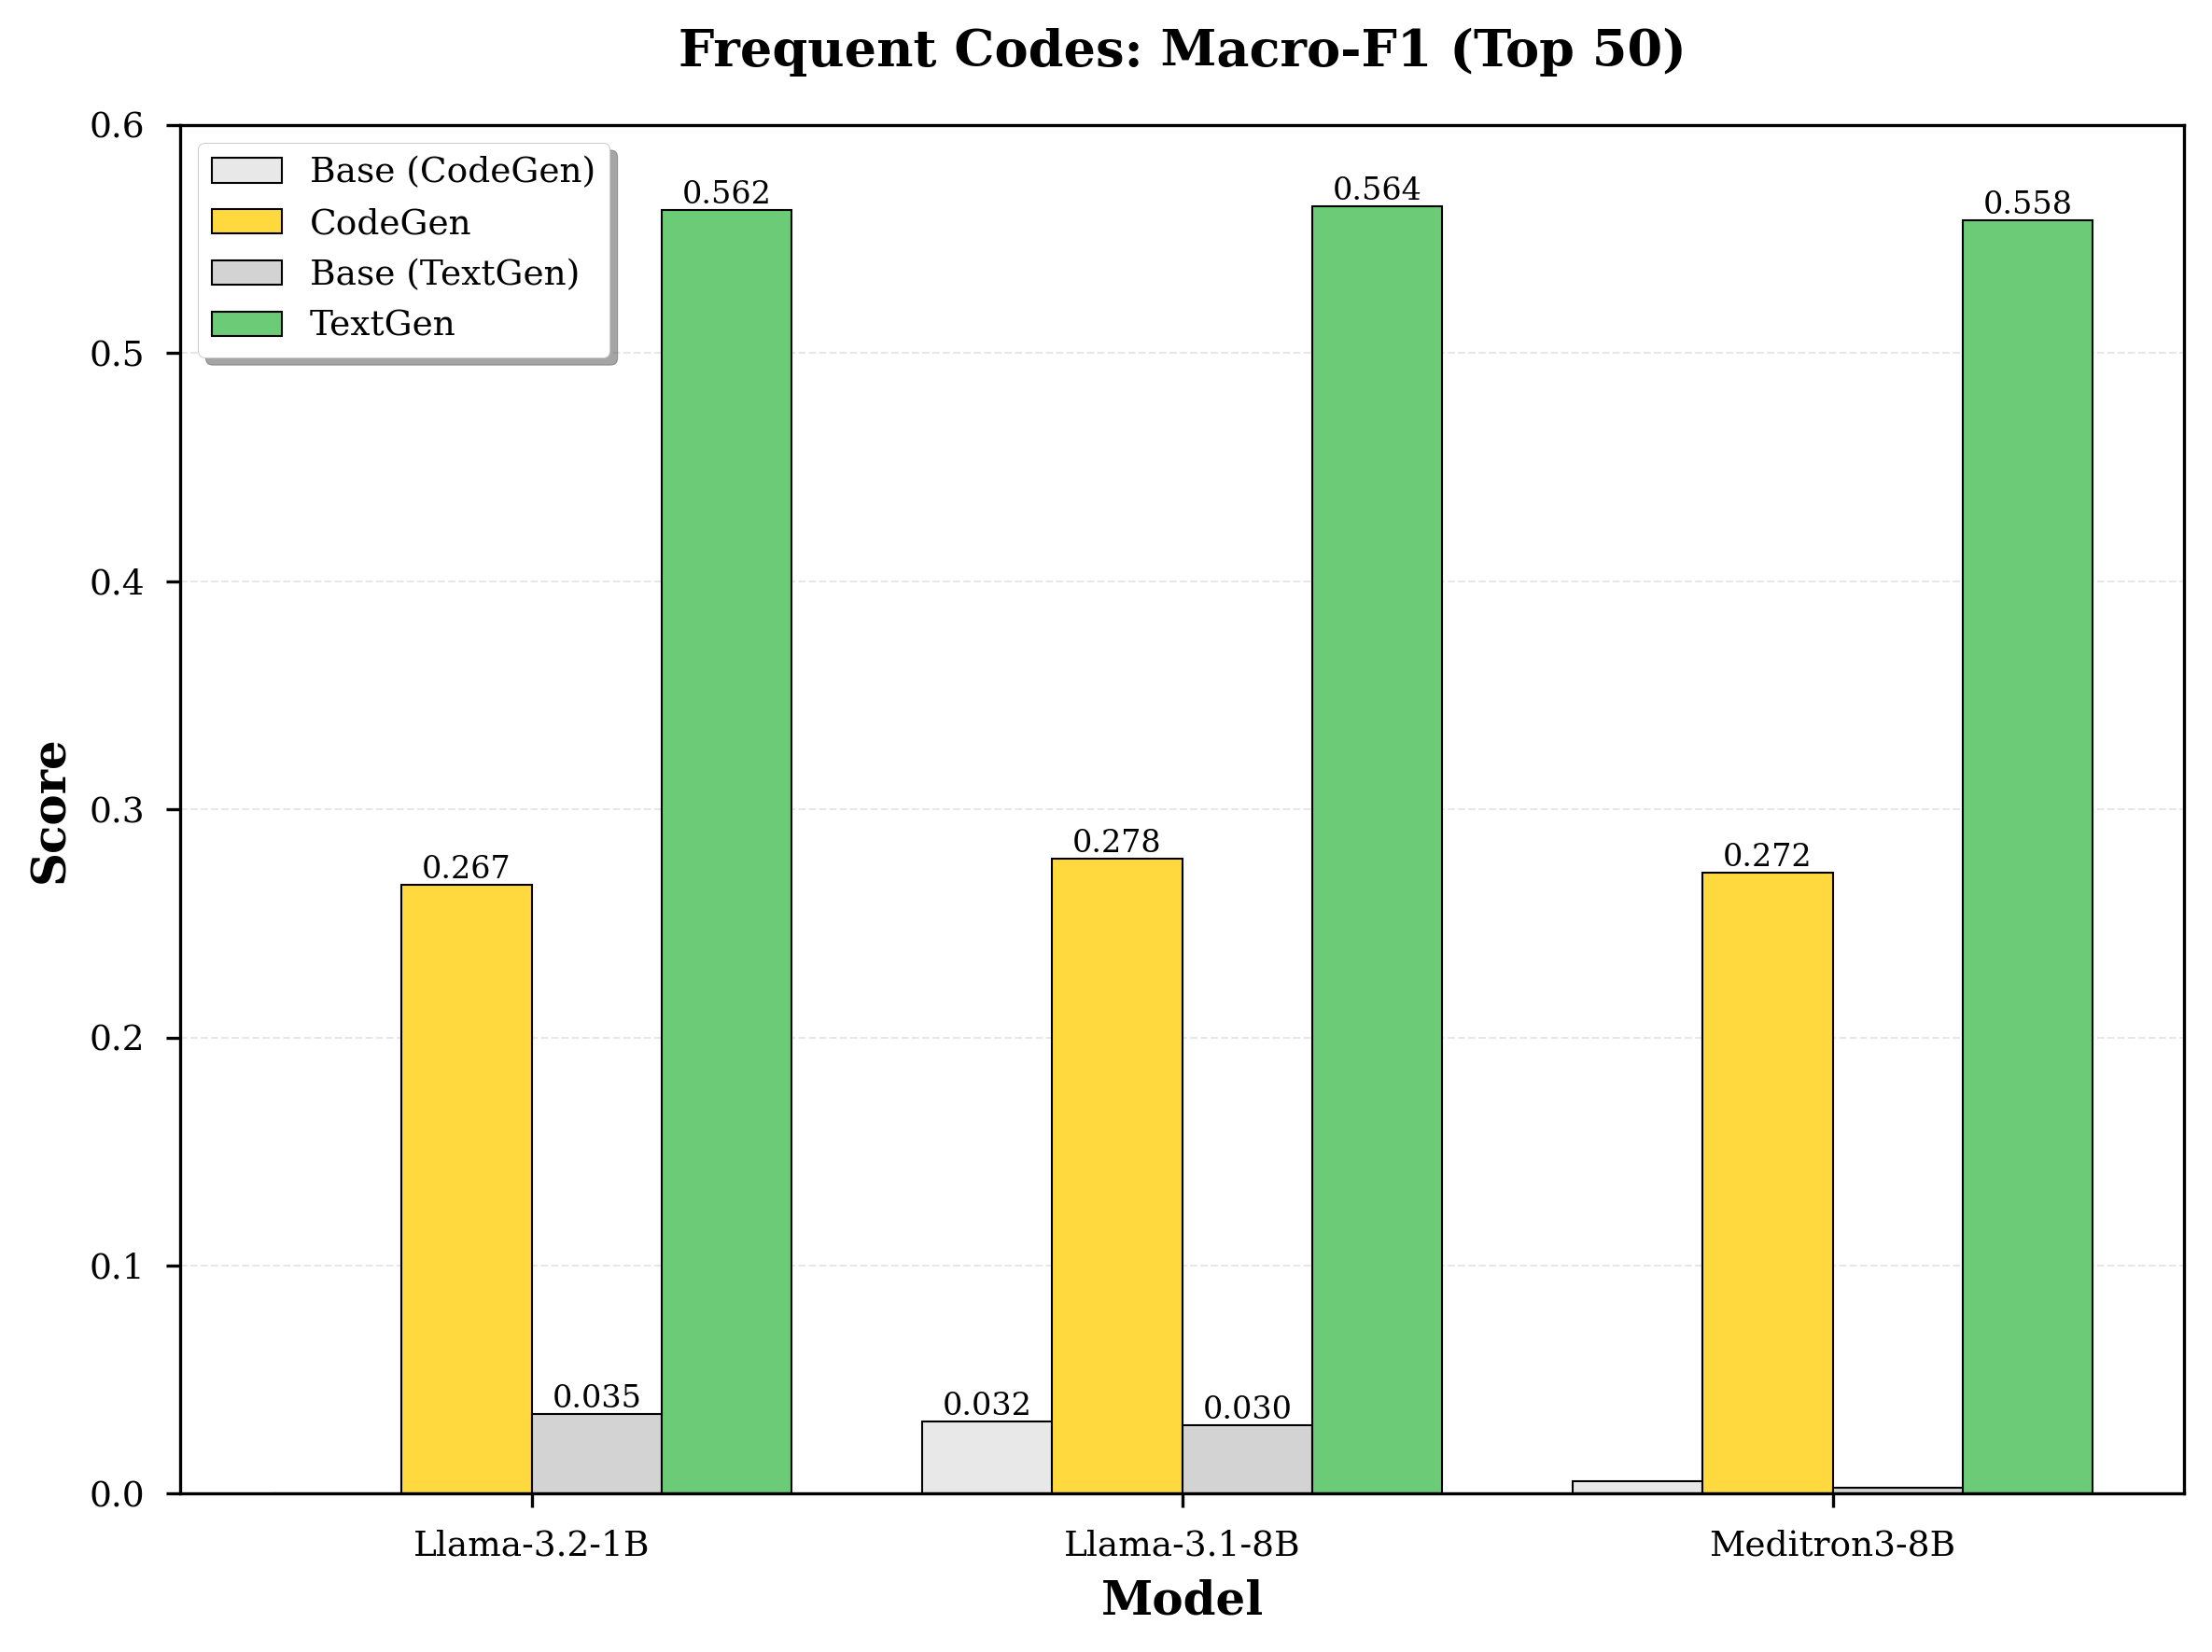
\includegraphics[width=\linewidth]{Images/Plots_thesis/top50_macro_f1.png}
        \caption{Top-50 macro-F1}
        \label{fig:task1-top50-macroF1}
    \end{subfigure}

    \vspace{0.3cm}

    % second row
    \begin{subfigure}{0.48\textwidth}
        \centering
        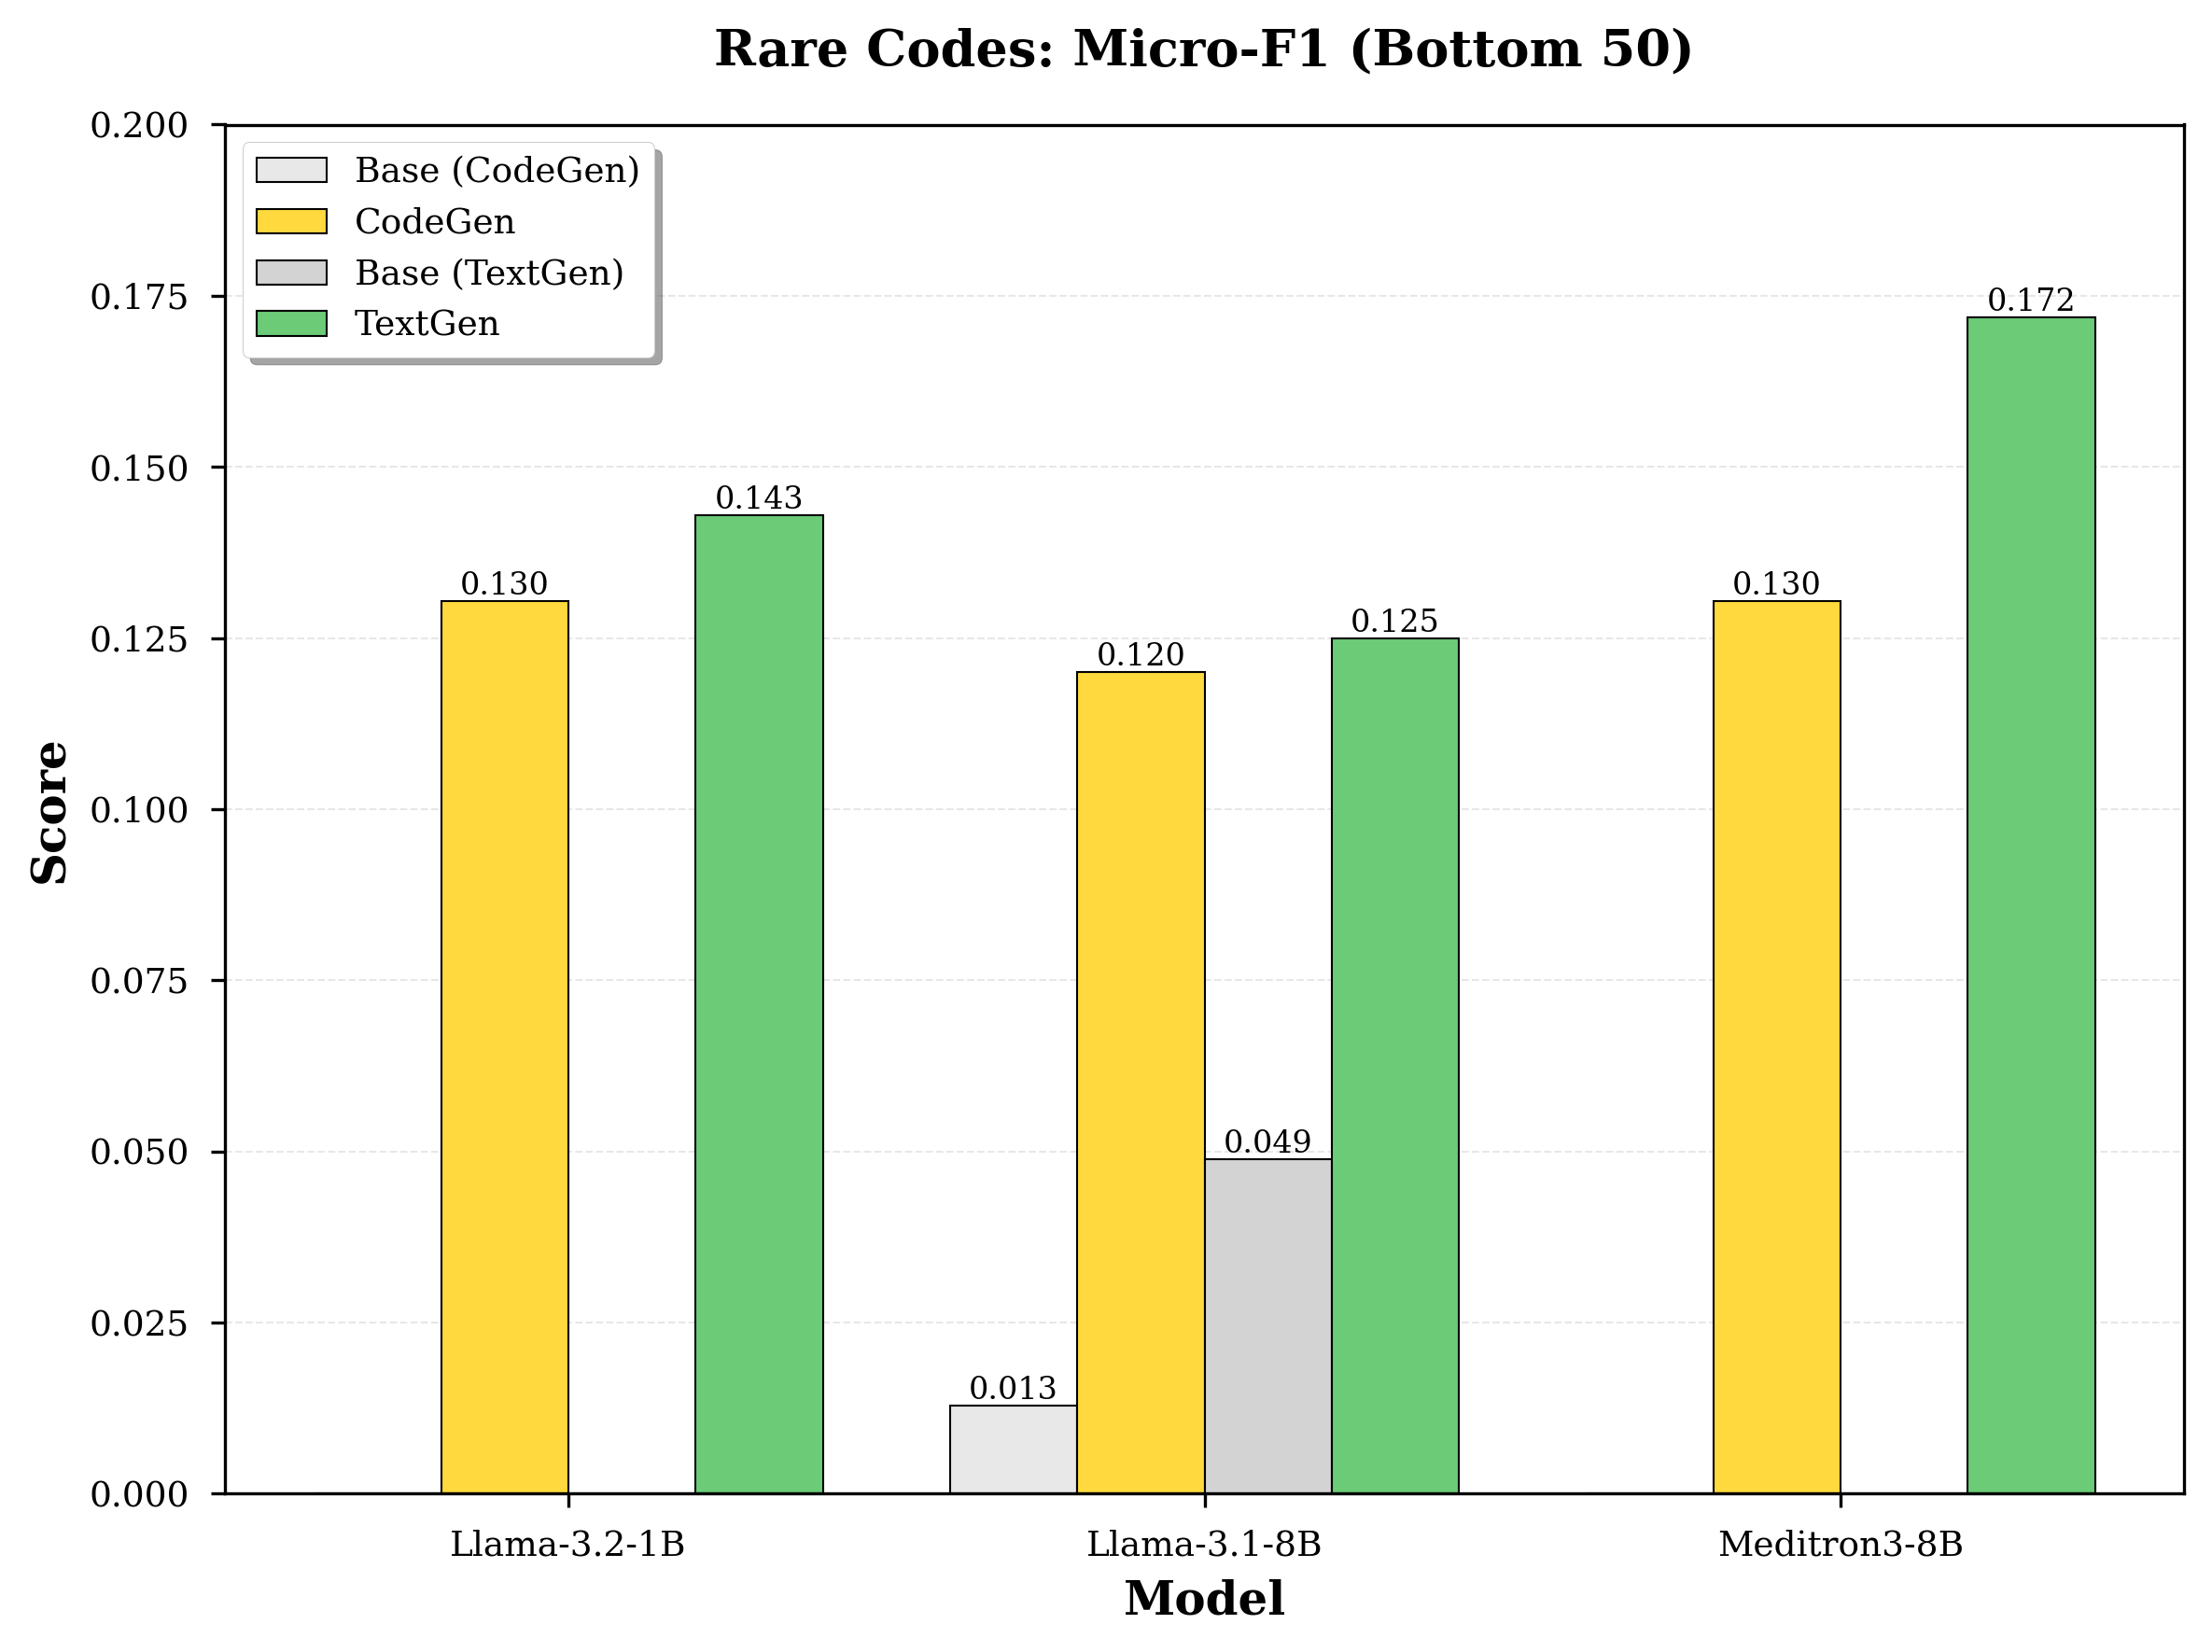
\includegraphics[width=\linewidth]{Images/Plots_thesis/bottom50_micro_f1.png}
        \caption{Bottom-50 micro-F1}
        \label{fig:task1-bottom50-microF1}
    \end{subfigure}\hfill
    \begin{subfigure}{0.48\textwidth}
        \centering
        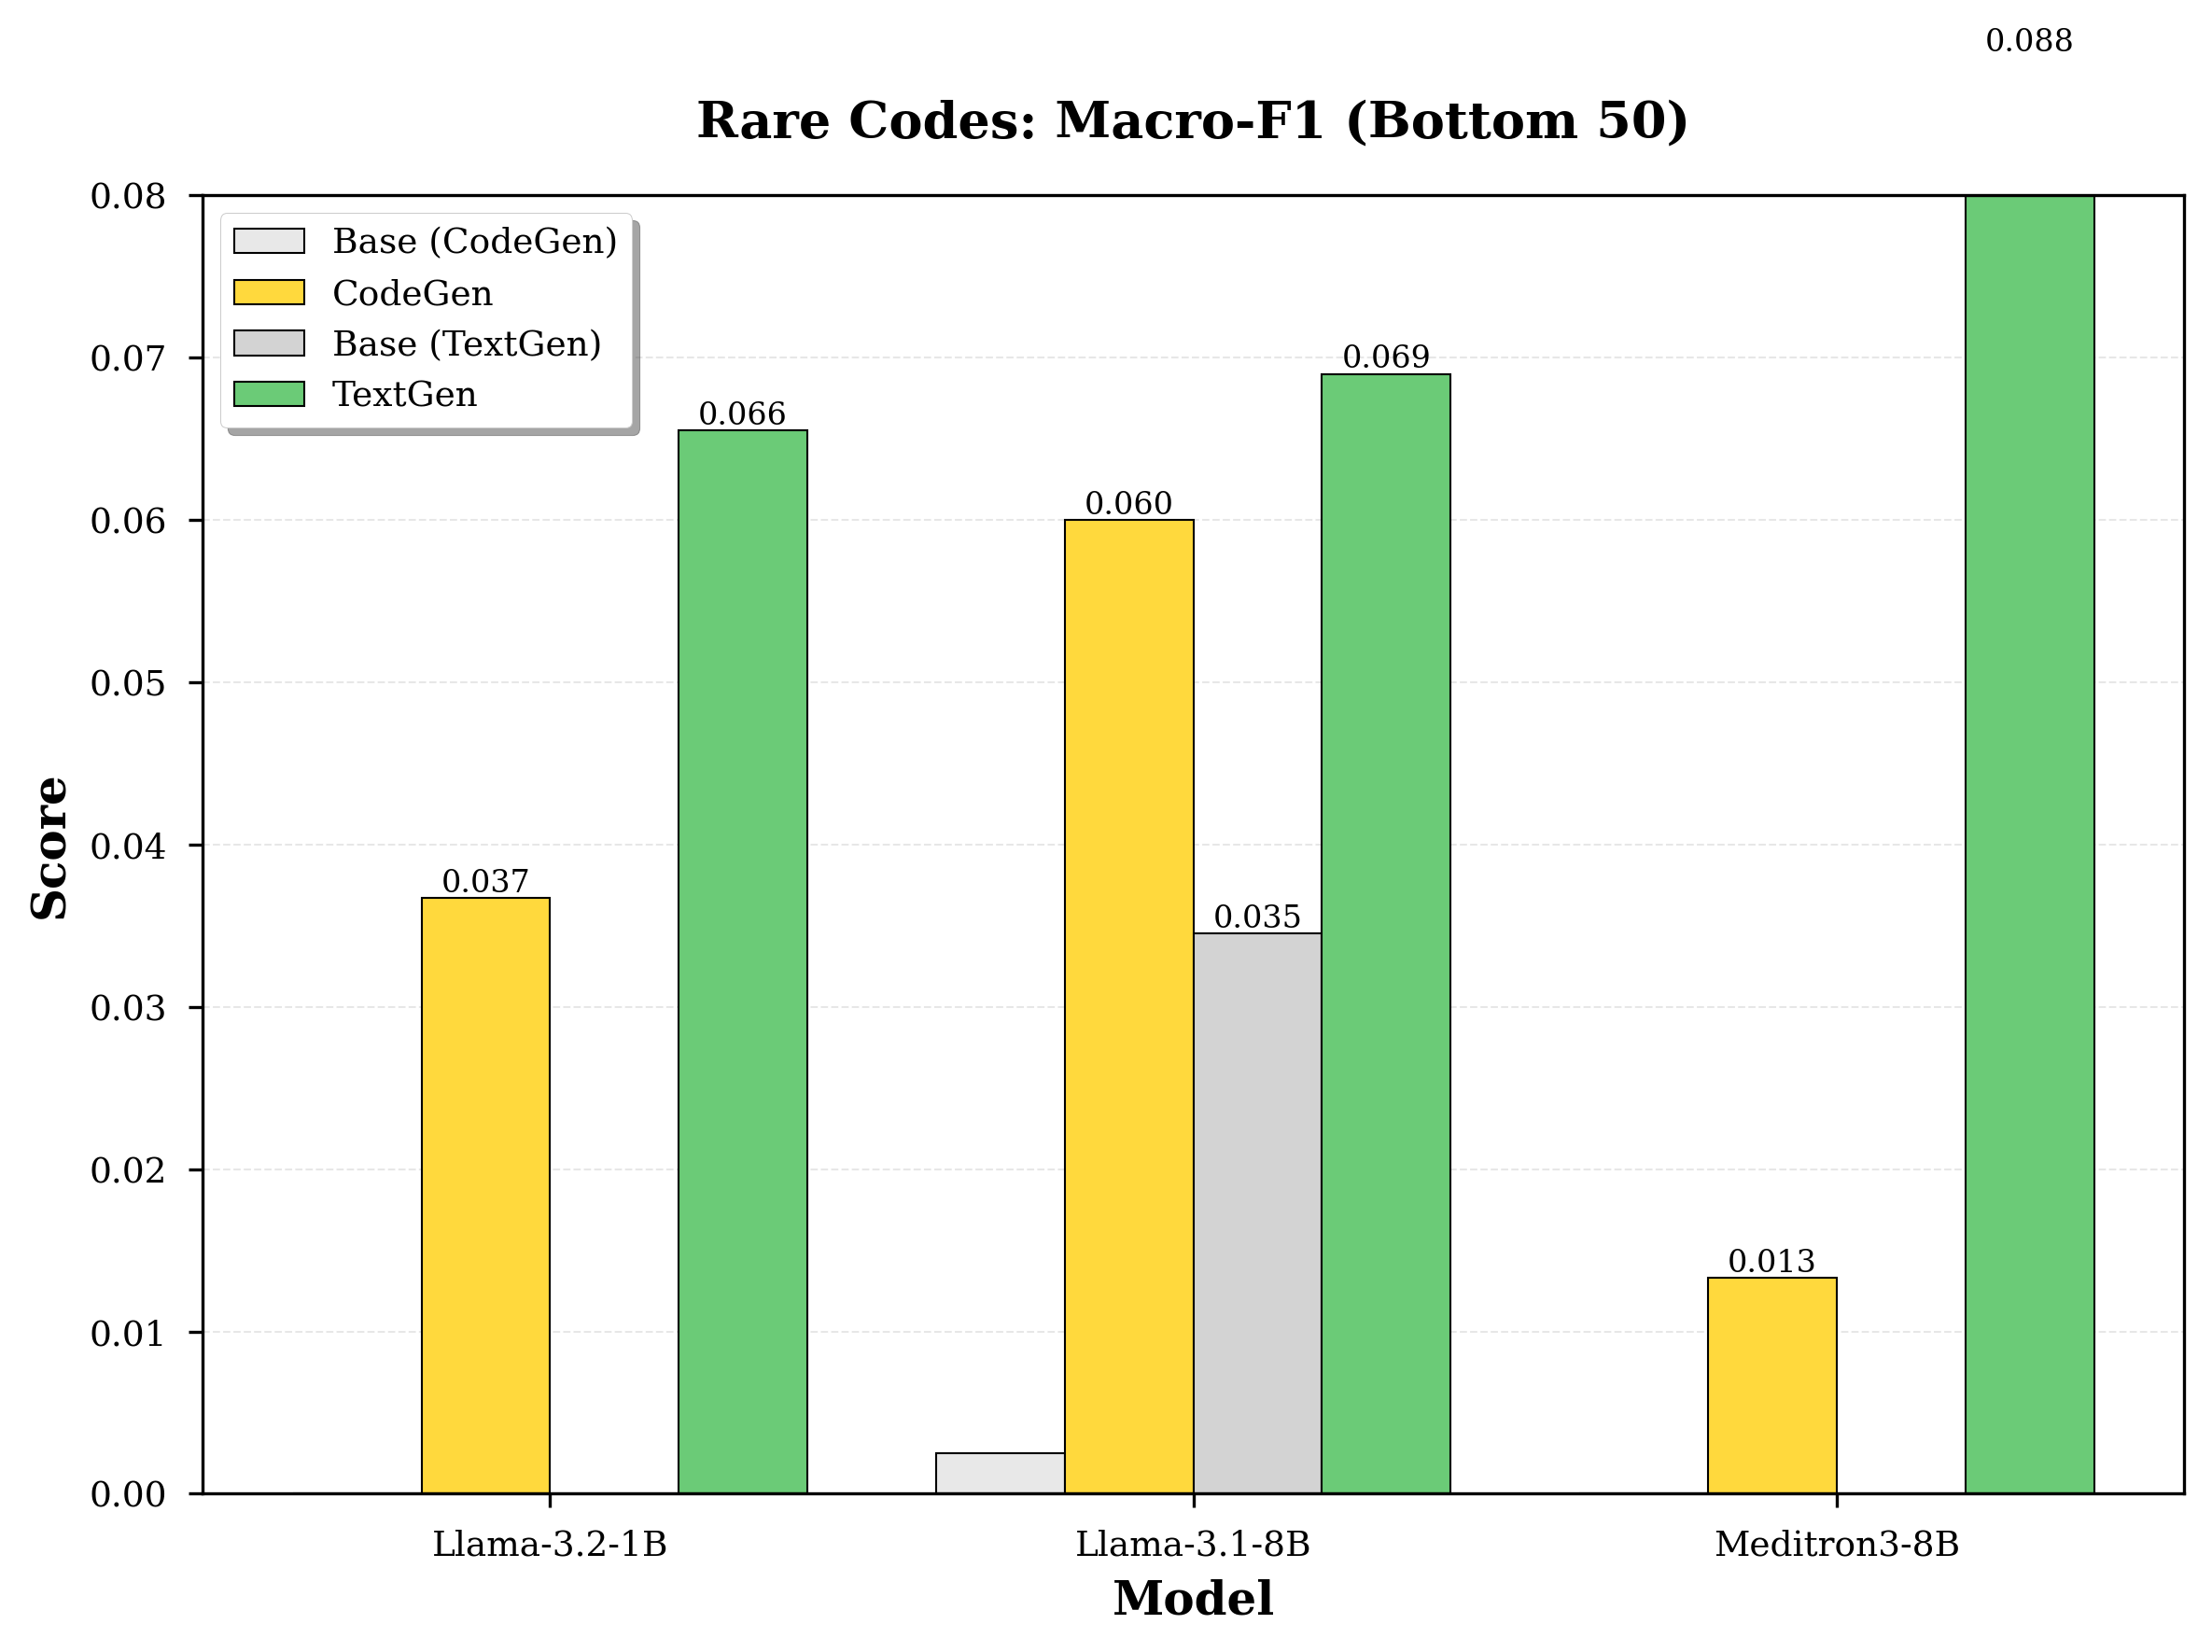
\includegraphics[width=\linewidth]{Images/Plots_thesis/bottom50_macro_f1.png}
        \caption{Bottom-50 macro-F1}
        \label{fig:task1-bottom50-macroF1}
    \end{subfigure}

    \caption{Task~1: Head-50 vs Tail-50 comparison (e.g., micro-F1 and macro-F1) across CodeGen vs TextGen and base model.}
    \label{fig:task1-headtail-metrics}
\end{figure}

% ============================================================
\subsection{Ablation: Augmenting KG Paths at Inference Only (No KG Training)}
\label{subsec:results-task1-kg-inference-only}

We next test whether structured knowledge helps \emph{without changing training}. Concretely, we take a strong fine-tuned TextGen baseline and \textbf{only modify inference} by injecting retrieved KG paths into the prompt. This is an ablation of \emph{prompt-time grounding}: the model sees KG context at test time, but it has never been trained to consume or rely on the KG section.

We report results for two retrieval scopes: \textbf{H1} and \textbf{H2}. Importantly, the baseline used for this ablation is evaluated with \textbf{no KG paths at inference}, providing a clean reference point for ``KG at inference-only''.

\paragraph{Overall code-level effect.}
Table~\ref{tab:task1-kg-inference-overall} shows that injecting KG paths \emph{at inference only} does \textbf{not} produce consistent gains in overall performance; across backbones, micro-F1 and macro-F1 are typically lower than the baseline without KG at inference. The degradation is most pronounced for the 1B backbone, suggesting increased sensitivity to prompt distribution shifts at smaller scale.

\begin{table}[t]
\centering
\caption{Task~1 inference-only KG ablation (overall code-level). Same fine-tuned TextGen checkpoint; only inference prompt differs.}
\label{tab:task1-kg-inference-overall}
\begin{tabular}{lcccccc}
\toprule
\textbf{Model} &
\multicolumn{2}{c}{\textbf{Baseline (no KG @ inf)}} &
\multicolumn{2}{c}{\textbf{+ KG H1 @ inf}} &
\multicolumn{2}{c}{\textbf{+ KG H2 @ inf}} \\
\cmidrule(lr){2-3}\cmidrule(lr){4-5}\cmidrule(lr){6-7}
& \textbf{Micro-F1} & \textbf{Macro-F1}
& \textbf{Micro-F1} & \textbf{Macro-F1}
& \textbf{Micro-F1} & \textbf{Macro-F1} \\
\midrule
Llama-3.2-1B   & 0.4313 & 0.2065 & 0.3764 & 0.1807 & 0.4056 & 0.1904 \\
Llama-3.1-8B   & 0.4585 & 0.2457 & 0.4441 & 0.2370 & 0.4510 & 0.2450 \\
Meditron3-8B   & 0.4556 & 0.2457 & 0.4440 & 0.2382 & 0.4527 & 0.2404 \\
\bottomrule
\end{tabular}
\end{table}

\paragraph{Why inference-only KG can fail.}
A plausible explanation is that na\"ively injecting KG paths introduces a \textbf{distribution shift} in the prompt: the model is not trained to treat KG paths as privileged evidence, and may (i) attend to irrelevant or noisy relations, (ii) allocate its limited 12-output budget to KG-correlated but incorrect hypotheses, or (iii) suffer from context dilution when long retrieval text competes with clinically salient spans from the note. This motivates the next step: \emph{train the model to use KG context}.

% ============================================================
\subsection{KG-Augmented Fine-Tuning (RAG-Style Variants)}
\label{subsec:results-task1-kg-rag}

Motivated by the weak and inconsistent behaviour of inference-only KG prompting, we move to \textbf{KG-augmented fine-tuning}: during training, prompts are enriched with retrieved KG paths so the model learns to condition on structured relations. At inference, the same retrieval mechanism is applied, yielding a RAG-style pipeline.

We evaluate two retrieval scopes (\textbf{H1} vs.\ \textbf{H2}) and two integration strategies (\textbf{Unweighted} vs.\ \textbf{Weighted}). The baseline for these comparisons is the fine-tuned TextGen model evaluated \textbf{without KG paths at inference} (as in Section~\ref{subsec:results-task1-kg-inference-only}). This makes the comparison strict: KG/RAG must outperform a strong baseline that is not exposed to potentially noisy KG text at test time.

\paragraph{Overall code-level performance.}
Table~\ref{tab:task1-rag-overall} shows that KG-augmented fine-tuning yields \textbf{consistent improvements} in micro-F1 and macro-F1 over the baseline across all backbones. Weighted variants are strongest overall, suggesting that relevance-controlled KG selection helps reduce noise and stabilise gains.

\begin{table}[t]
\centering
\caption{Task~1 overall code-level metrics for KG-augmented (RAG) variants vs.\ Baseline TextGen (no KG at inference). Test set evaluation.}
\label{tab:task1-rag-overall}
\resizebox{\textwidth}{!}{
\begin{tabular}{llcccccc}
\toprule
\textbf{Model} & \textbf{Method} & \textbf{Micro-F1} & \textbf{Macro-F1} & \textbf{Micro-P} & \textbf{Macro-P} & \textbf{Micro-R} & \textbf{Macro-R} \\
\midrule
Llama-3.2-1B & H1 Unweighted & 0.4452 & 0.2134 & 0.5190 & 0.2862 & 0.3891 & 0.1941 \\
Llama-3.2-1B & H1 Weighted   & \textbf{0.4749} & \textbf{0.2368} & 0.5419 & 0.3068 & 0.4230 & 0.2289 \\
Llama-3.2-1B & H2 Unweighted & 0.4407 & 0.2143 & 0.5156 & 0.2888 & 0.3842 & 0.1940 \\
Llama-3.2-1B & H2 Weighted   & 0.4726 & 0.2333 & 0.5462 & 0.3067 & 0.4168 & 0.2234 \\
Llama-3.2-1B & Baseline TextGen (no KG @ inf) & 0.4313 & 0.2065 & 0.5084 & 0.2540 & 0.3745 & 0.1740 \\
\midrule
Llama-3.1-8B & H1 Unweighted & 0.4732 & 0.2546 & 0.5464 & 0.3349 & 0.4168 & 0.2406 \\
Llama-3.1-8B & H1 Weighted   & \textbf{0.5029} & \textbf{0.2762} & 0.5770 & 0.3565 & 0.4459 & 0.2615 \\
Llama-3.1-8B & H2 Unweighted & 0.4699 & 0.2558 & 0.5426 & 0.3334 & 0.4139 & 0.2426 \\
Llama-3.1-8B & H2 Weighted   & 0.4998 & 0.2724 & 0.5739 & 0.3541 & 0.4429 & 0.2581 \\
Llama-3.1-8B & Baseline TextGen (no KG @ inf) & 0.4585 & 0.2457 & 0.5140 & 0.3338 & 0.4142 & 0.2400 \\
\midrule
Meditron3-8B & H1 Unweighted & 0.4700 & 0.2593 & 0.5436 & 0.3424 & 0.4135 & 0.2479 \\
Meditron3-8B & H1 Weighted   & \textbf{0.5036} & \textbf{0.2793} & 0.5765 & 0.3628 & 0.4473 & 0.2662 \\
Meditron3-8B & H2 Unweighted & 0.4736 & 0.2563 & 0.5499 & 0.3354 & 0.4153 & 0.2433 \\
Meditron3-8B & H2 Weighted   & 0.5023 & 0.2750 & 0.5792 & 0.3519 & 0.4437 & 0.2619 \\
Meditron3-8B & Baseline TextGen (no KG @ inf) & 0.4556 & 0.2457 & 0.5119 & 0.3295 & 0.4135 & 0.2395 \\
\bottomrule
\end{tabular}}
\end{table}

\begin{figure}[t]
    \centering
    % first row
    \begin{subfigure}{0.48\textwidth}
        \centering
        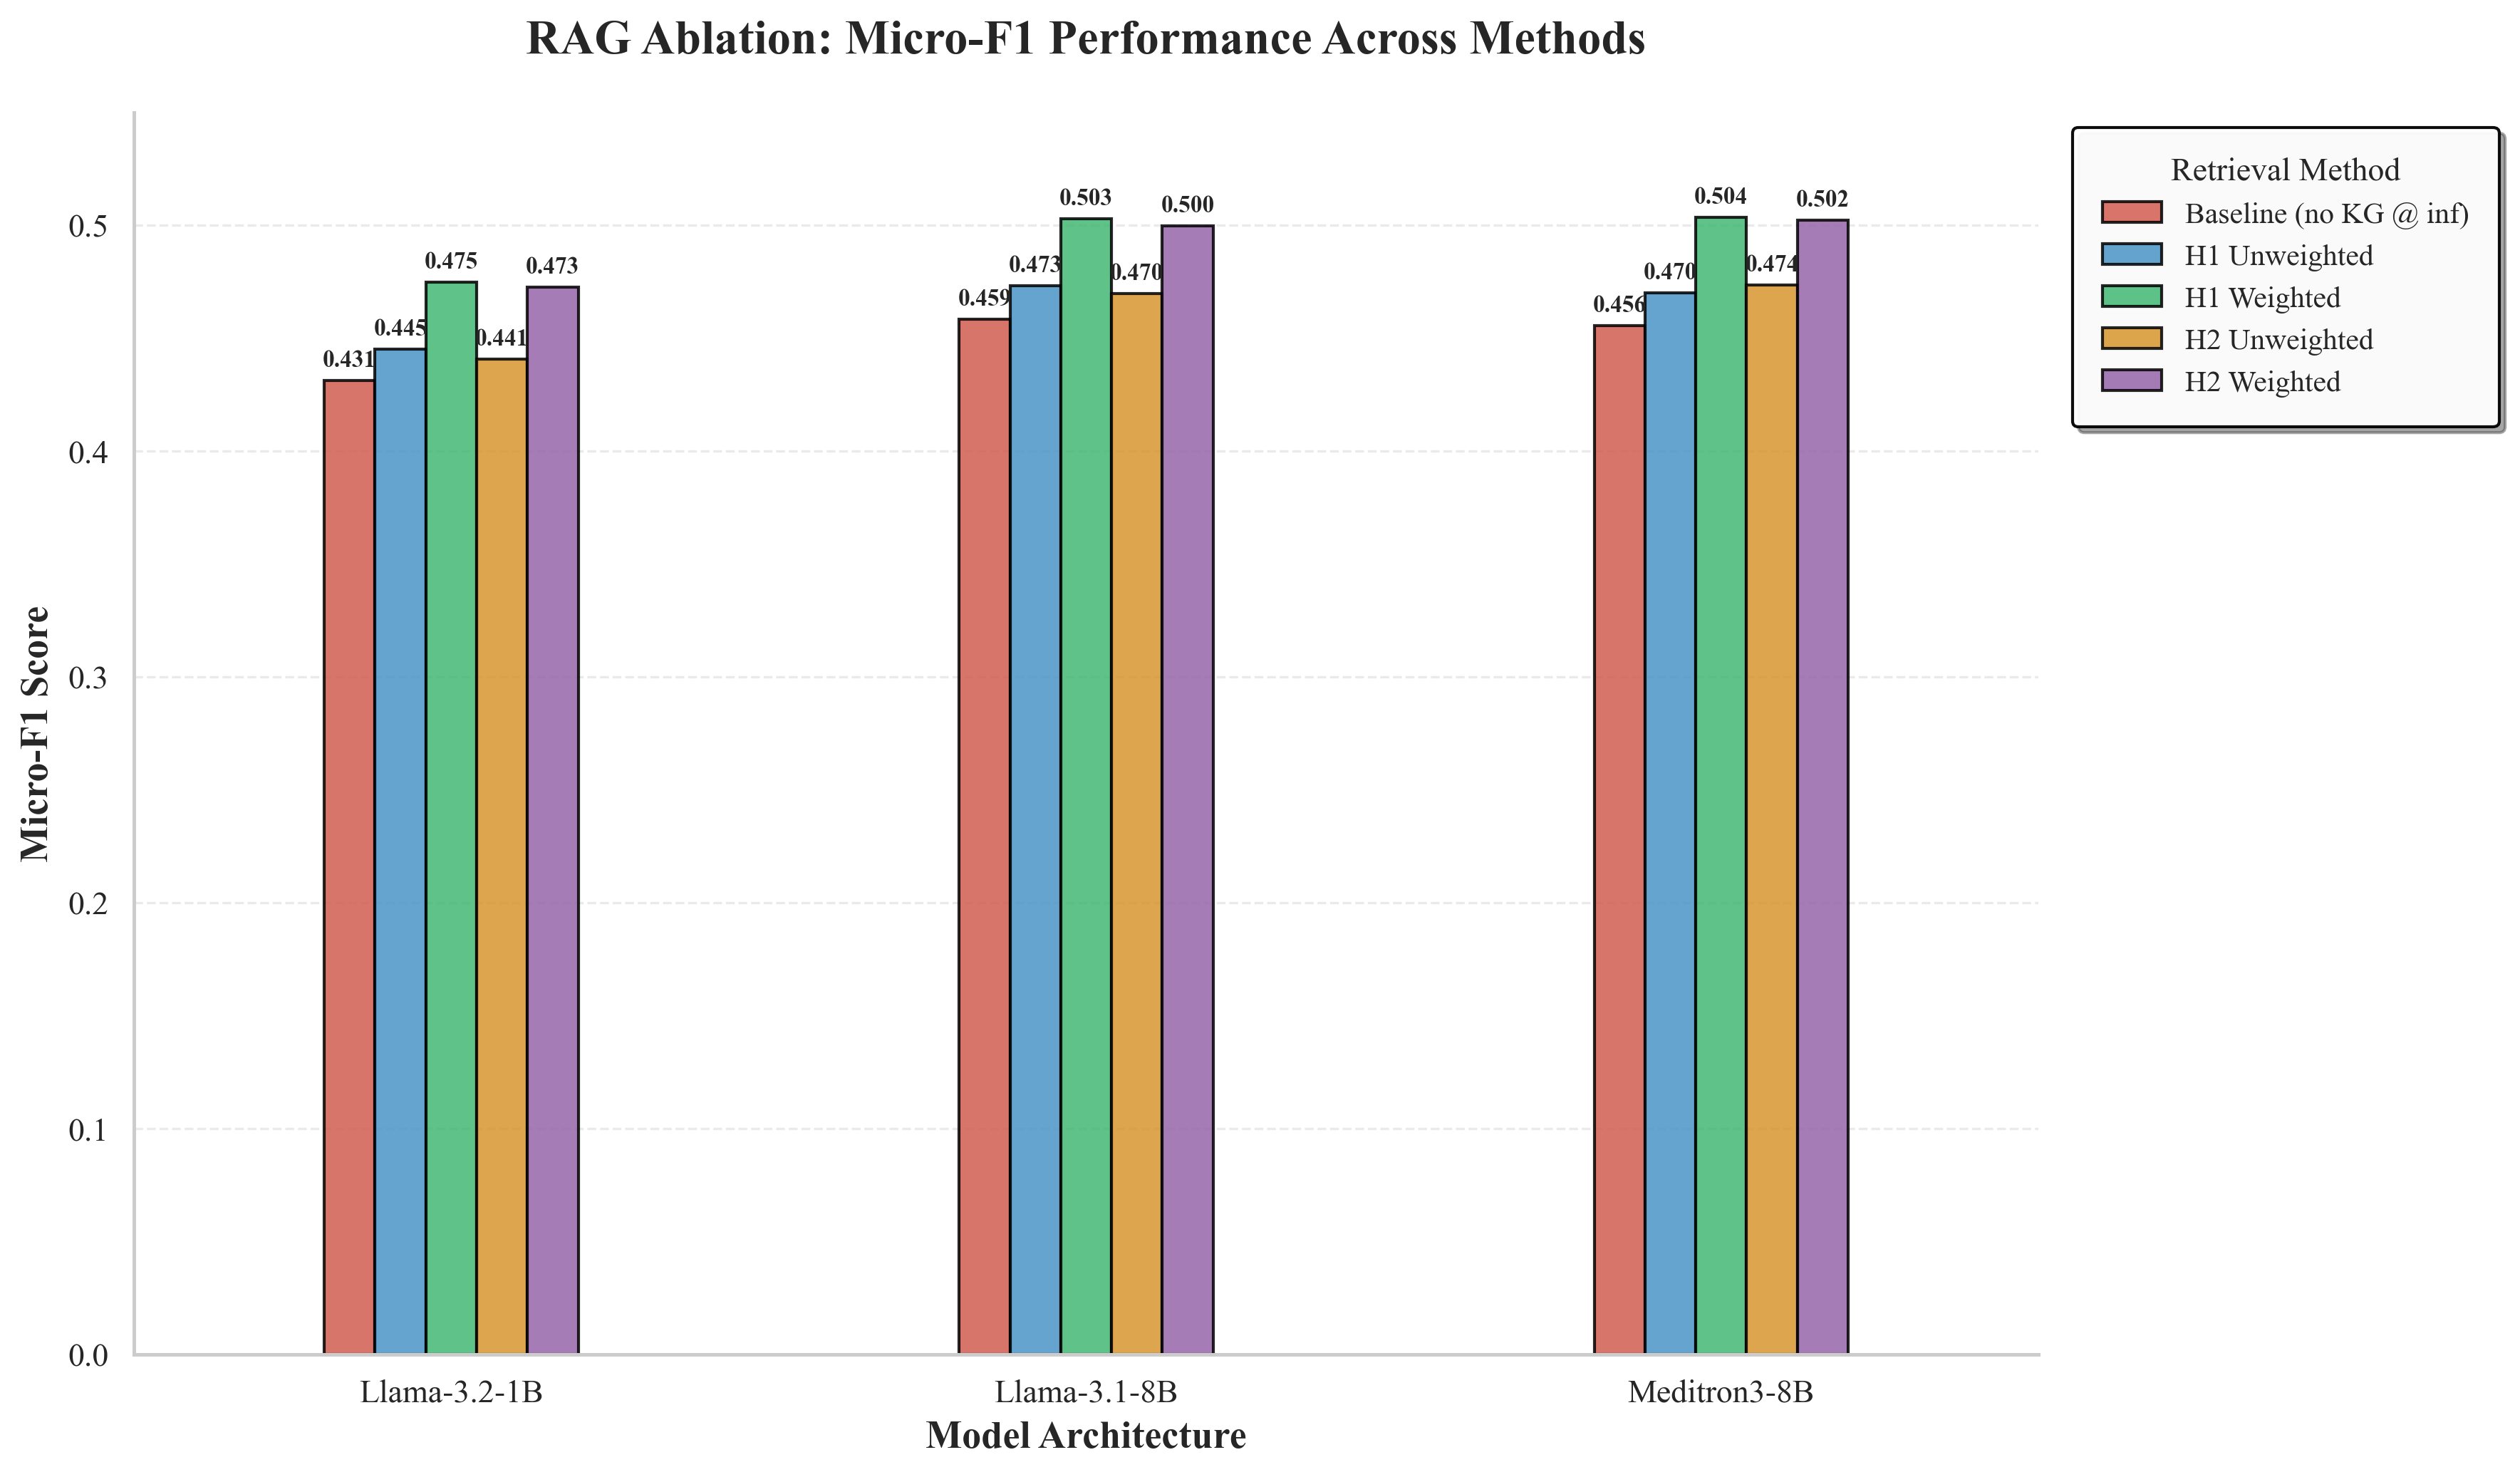
\includegraphics[width=\linewidth]{Images/h1vh2vbase/micro_f1.png}
        \caption{micro-F1}
        \label{fig:task1-h1vh2vbase-microF1}
    \end{subfigure}\hfill
    \begin{subfigure}{0.48\textwidth}
        \centering
        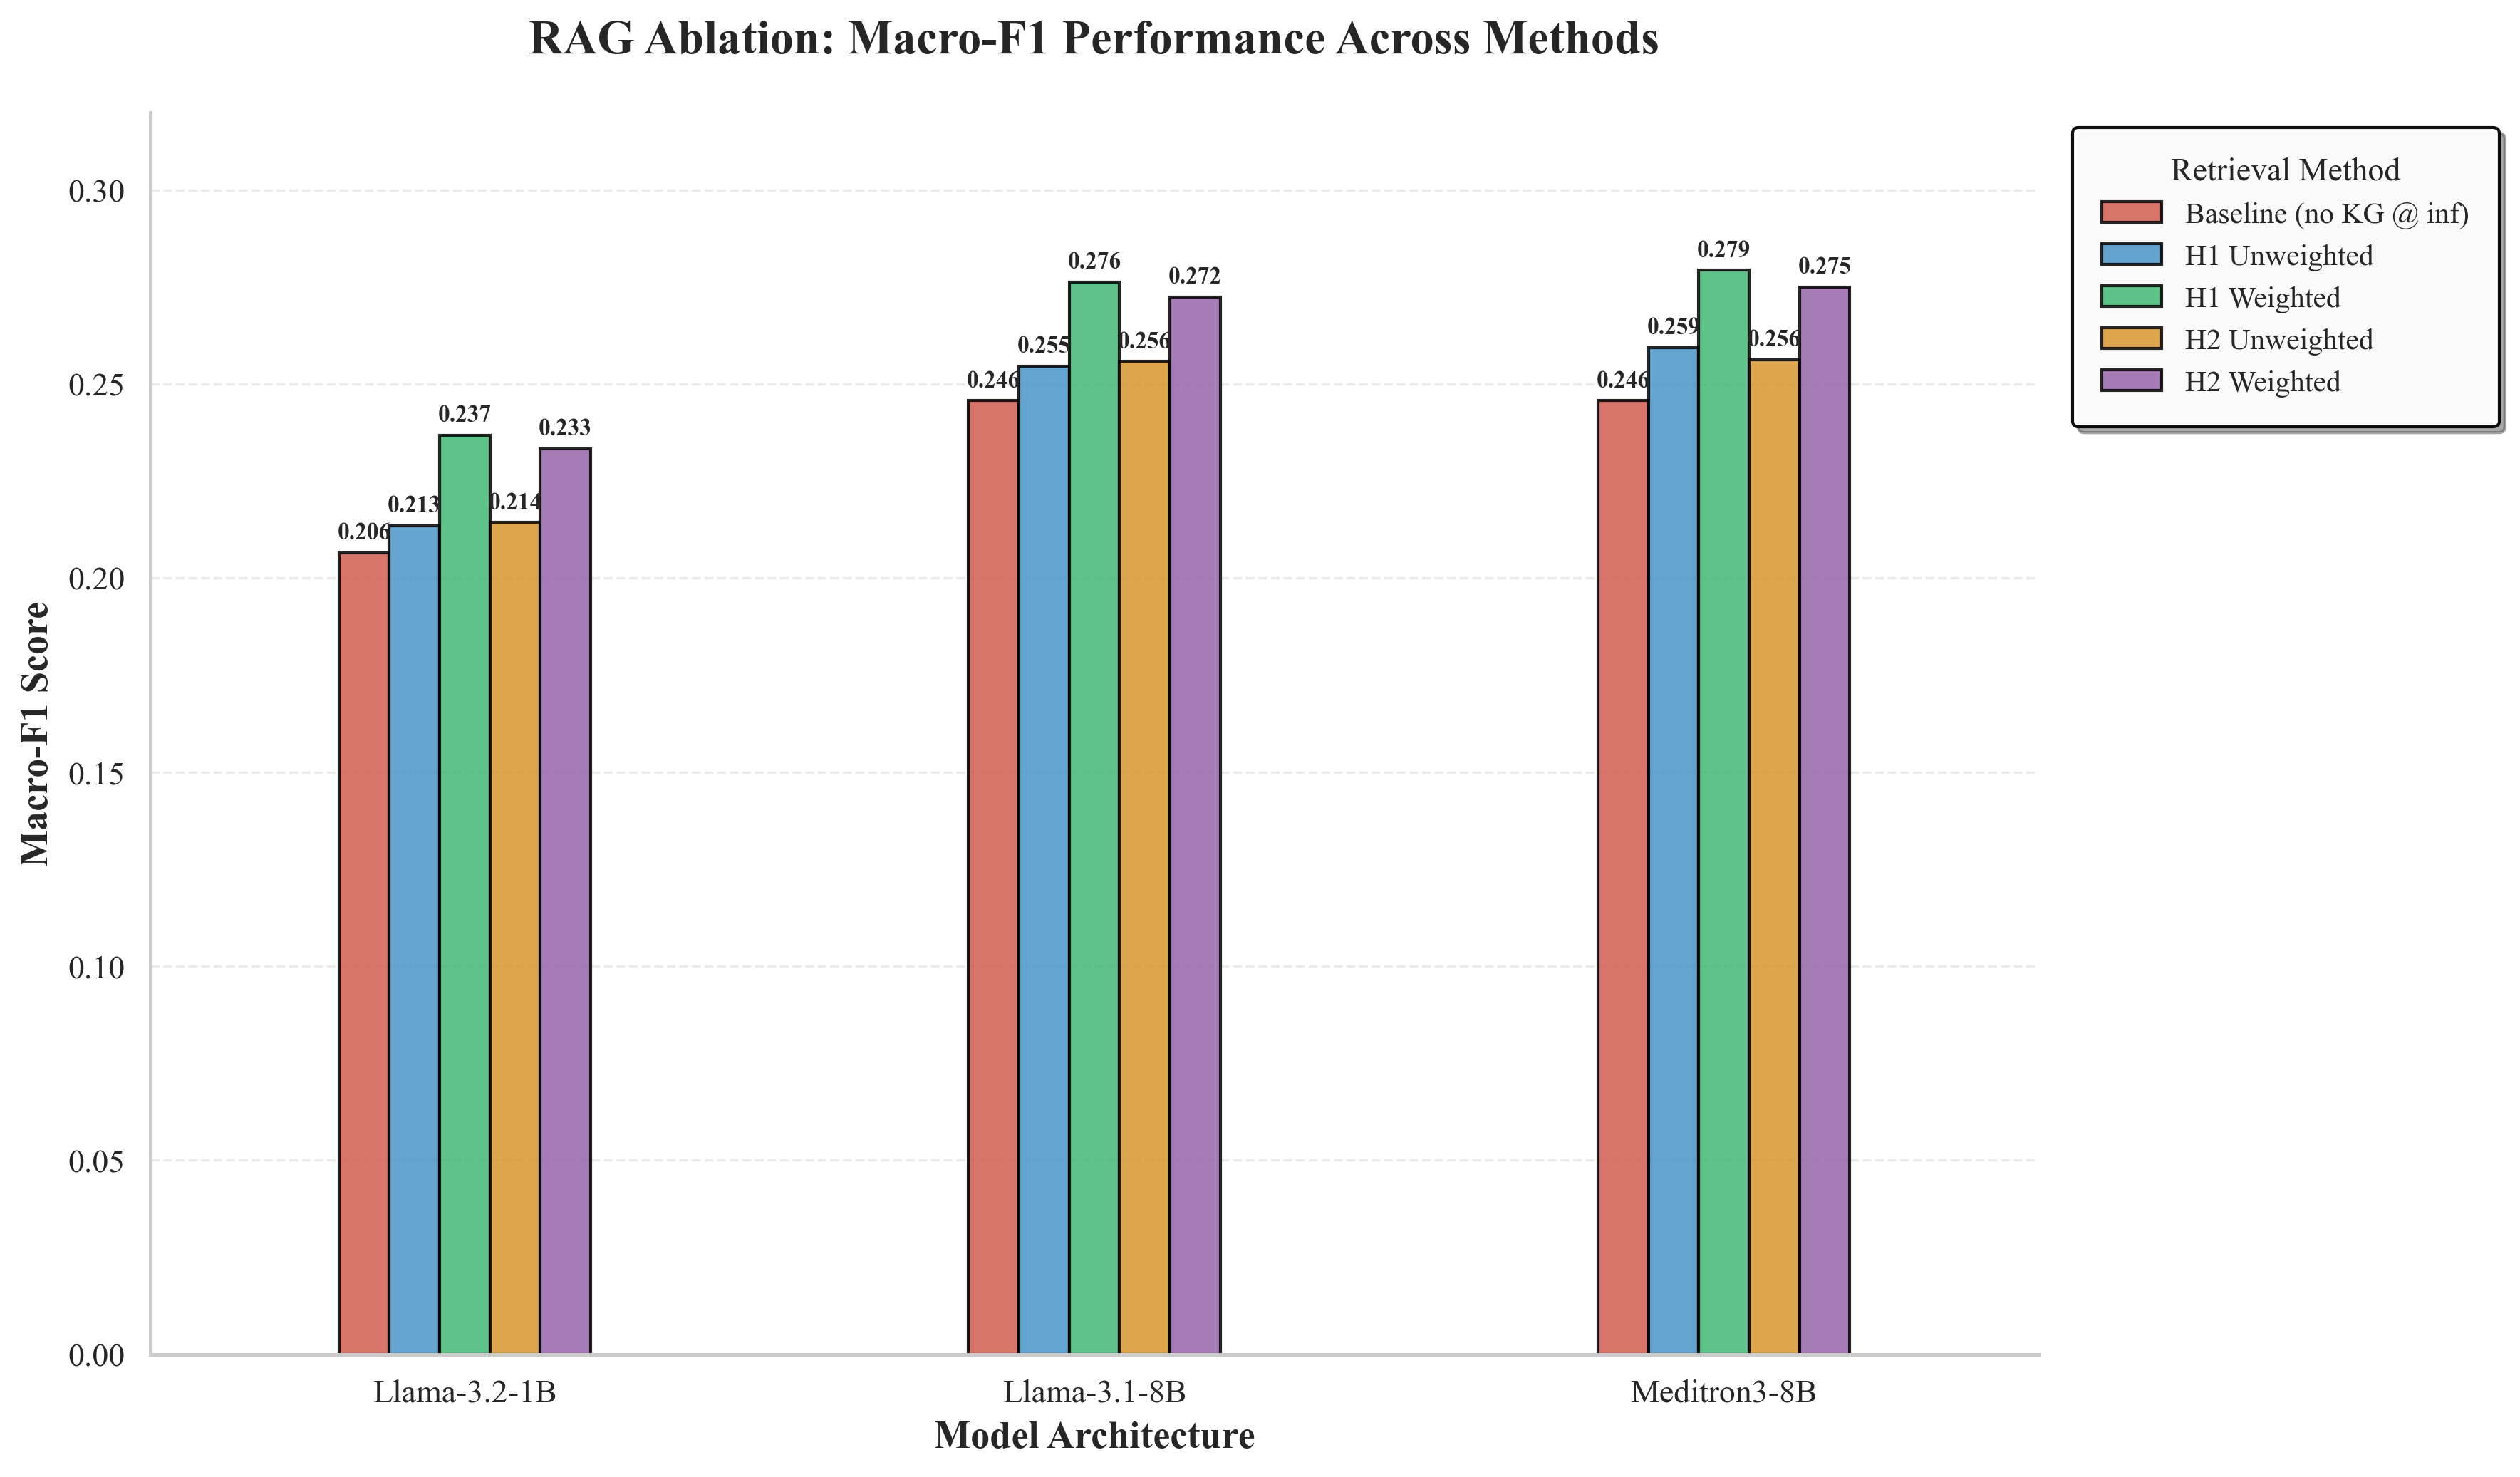
\includegraphics[width=\linewidth]{Images/h1vh2vbase/macro_f1.png}
        \caption{macro-F1}
        \label{fig:task1-h1vh2vbase-macroF1}
    \end{subfigure}

    \vspace{0.3cm}

    % second row
    \begin{subfigure}{0.48\textwidth}
        \centering
        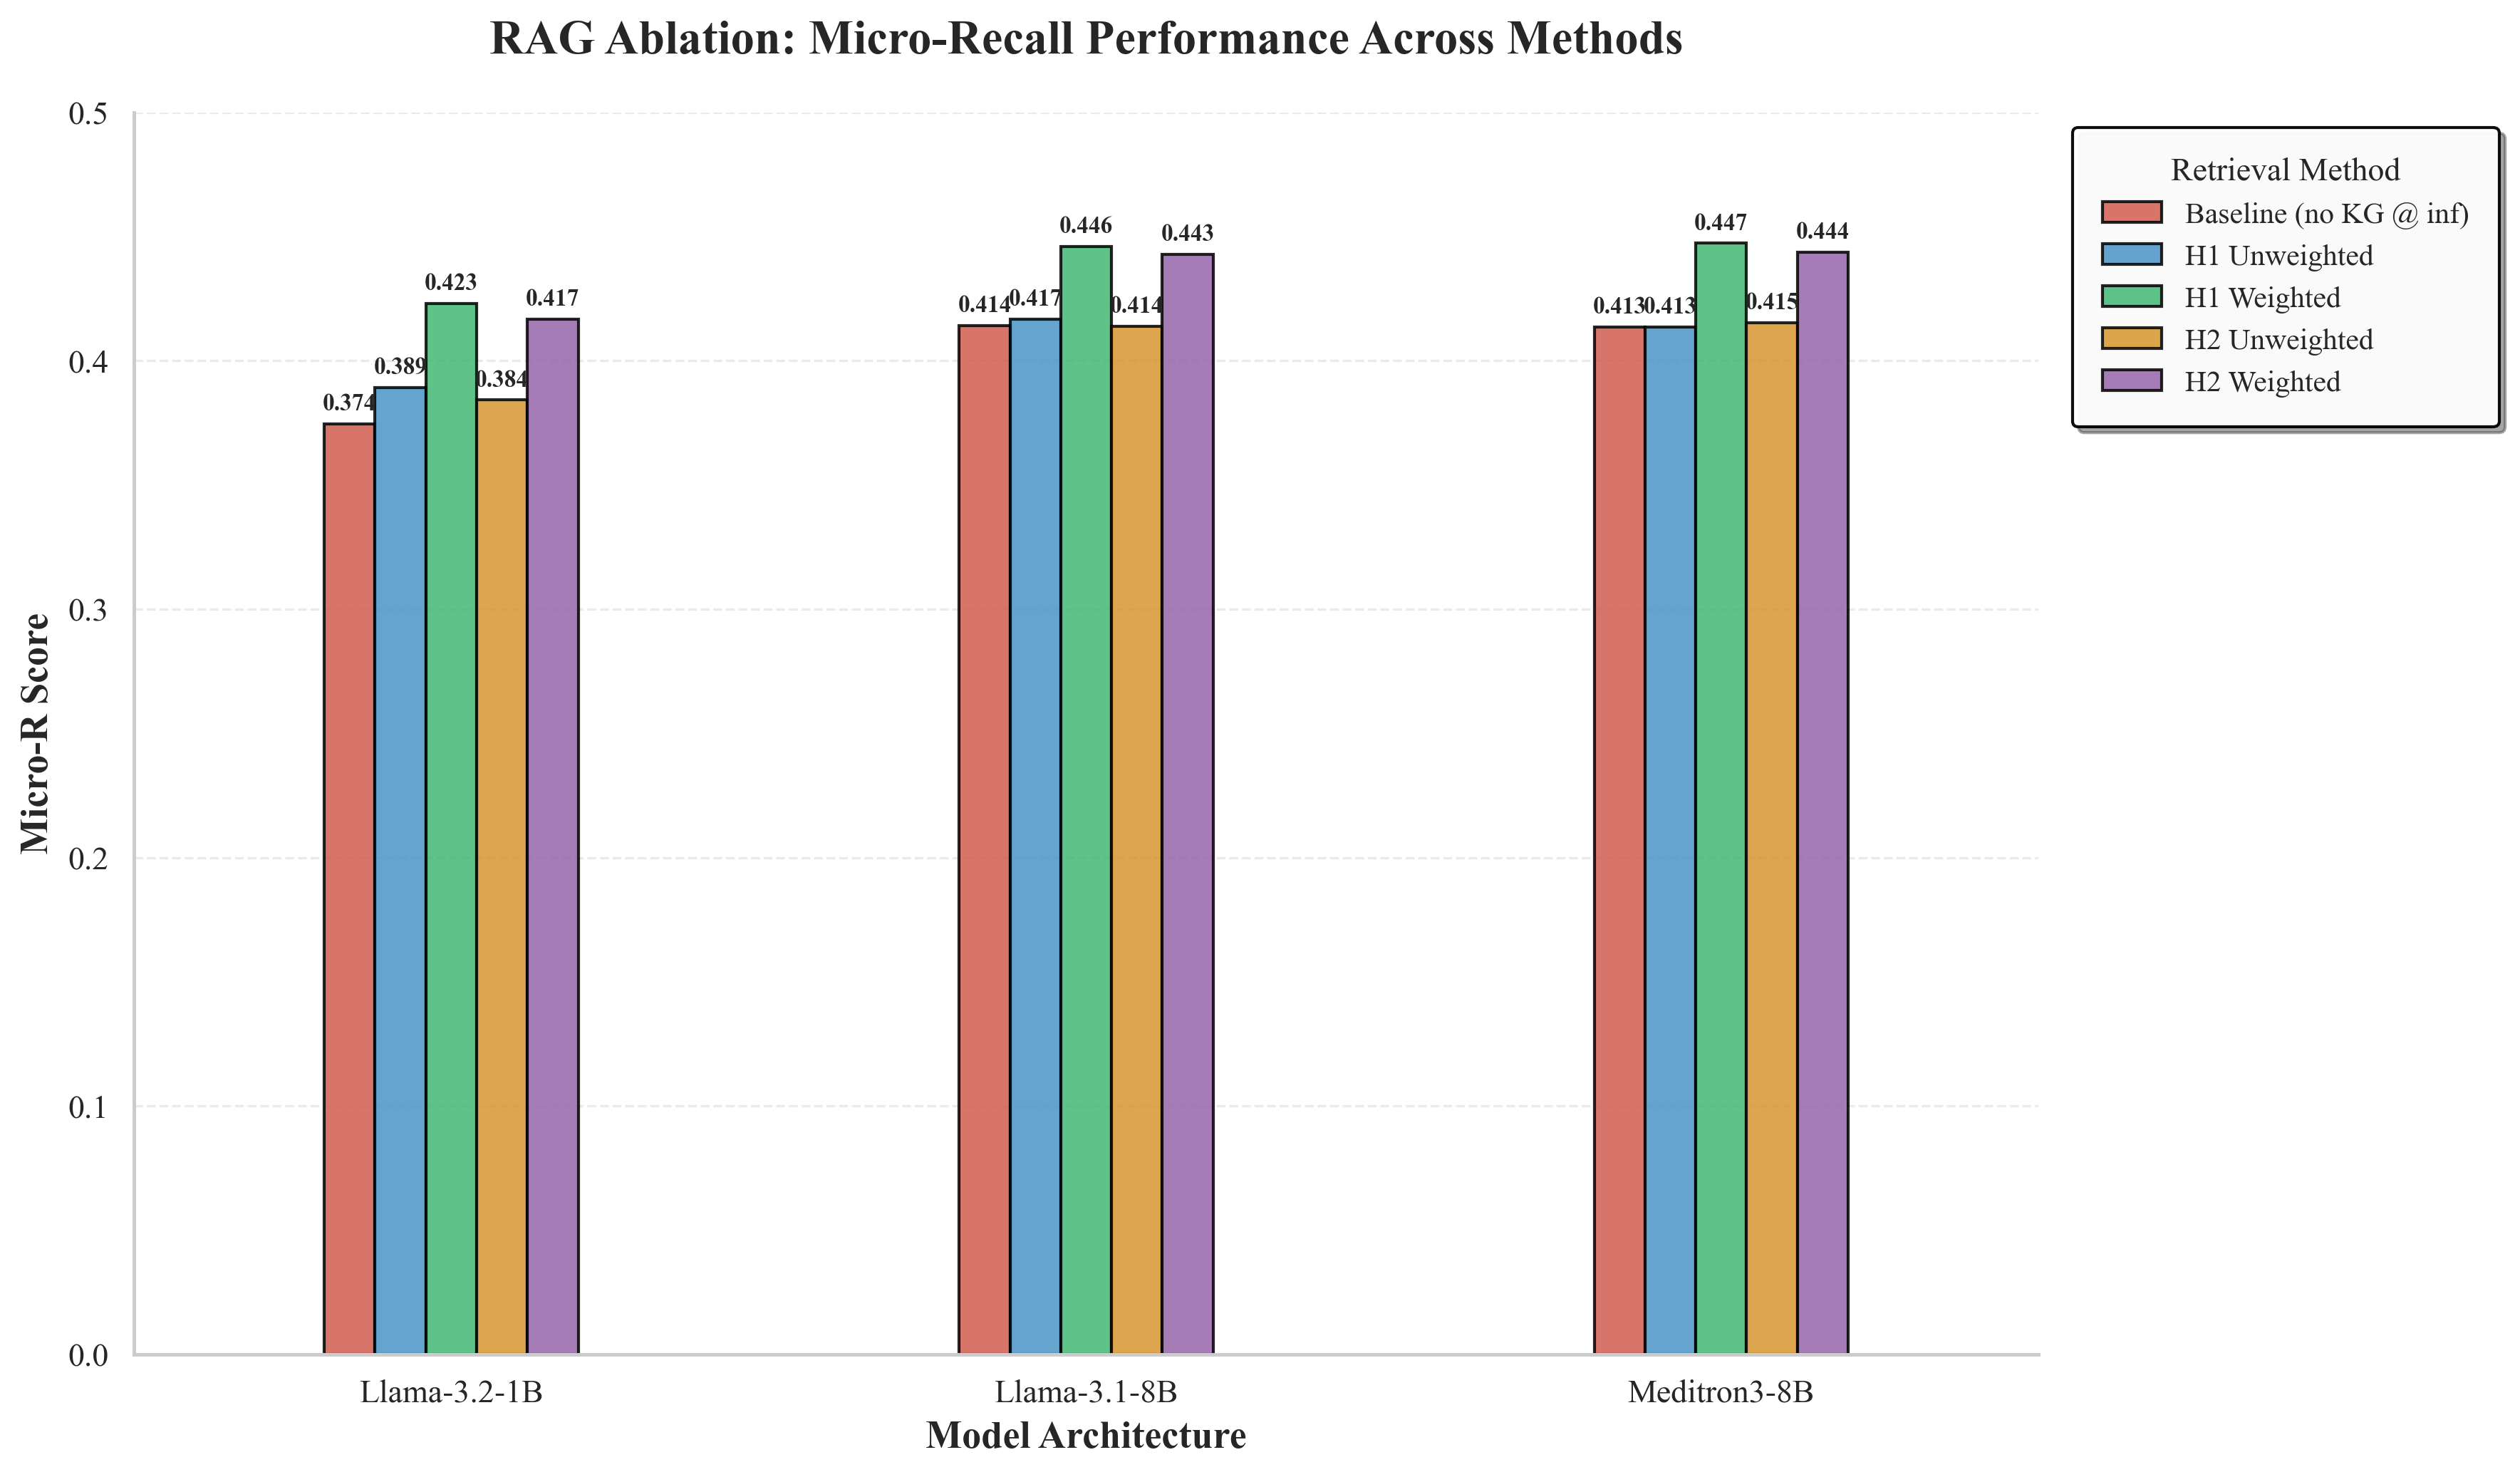
\includegraphics[width=\linewidth]{Images/h1vh2vbase/micro_recall.png}
        \caption{micro-recall}
        \label{fig:task1-bottom50-microRecall}
    \end{subfigure}\hfill
    \begin{subfigure}{0.48\textwidth}
        \centering
        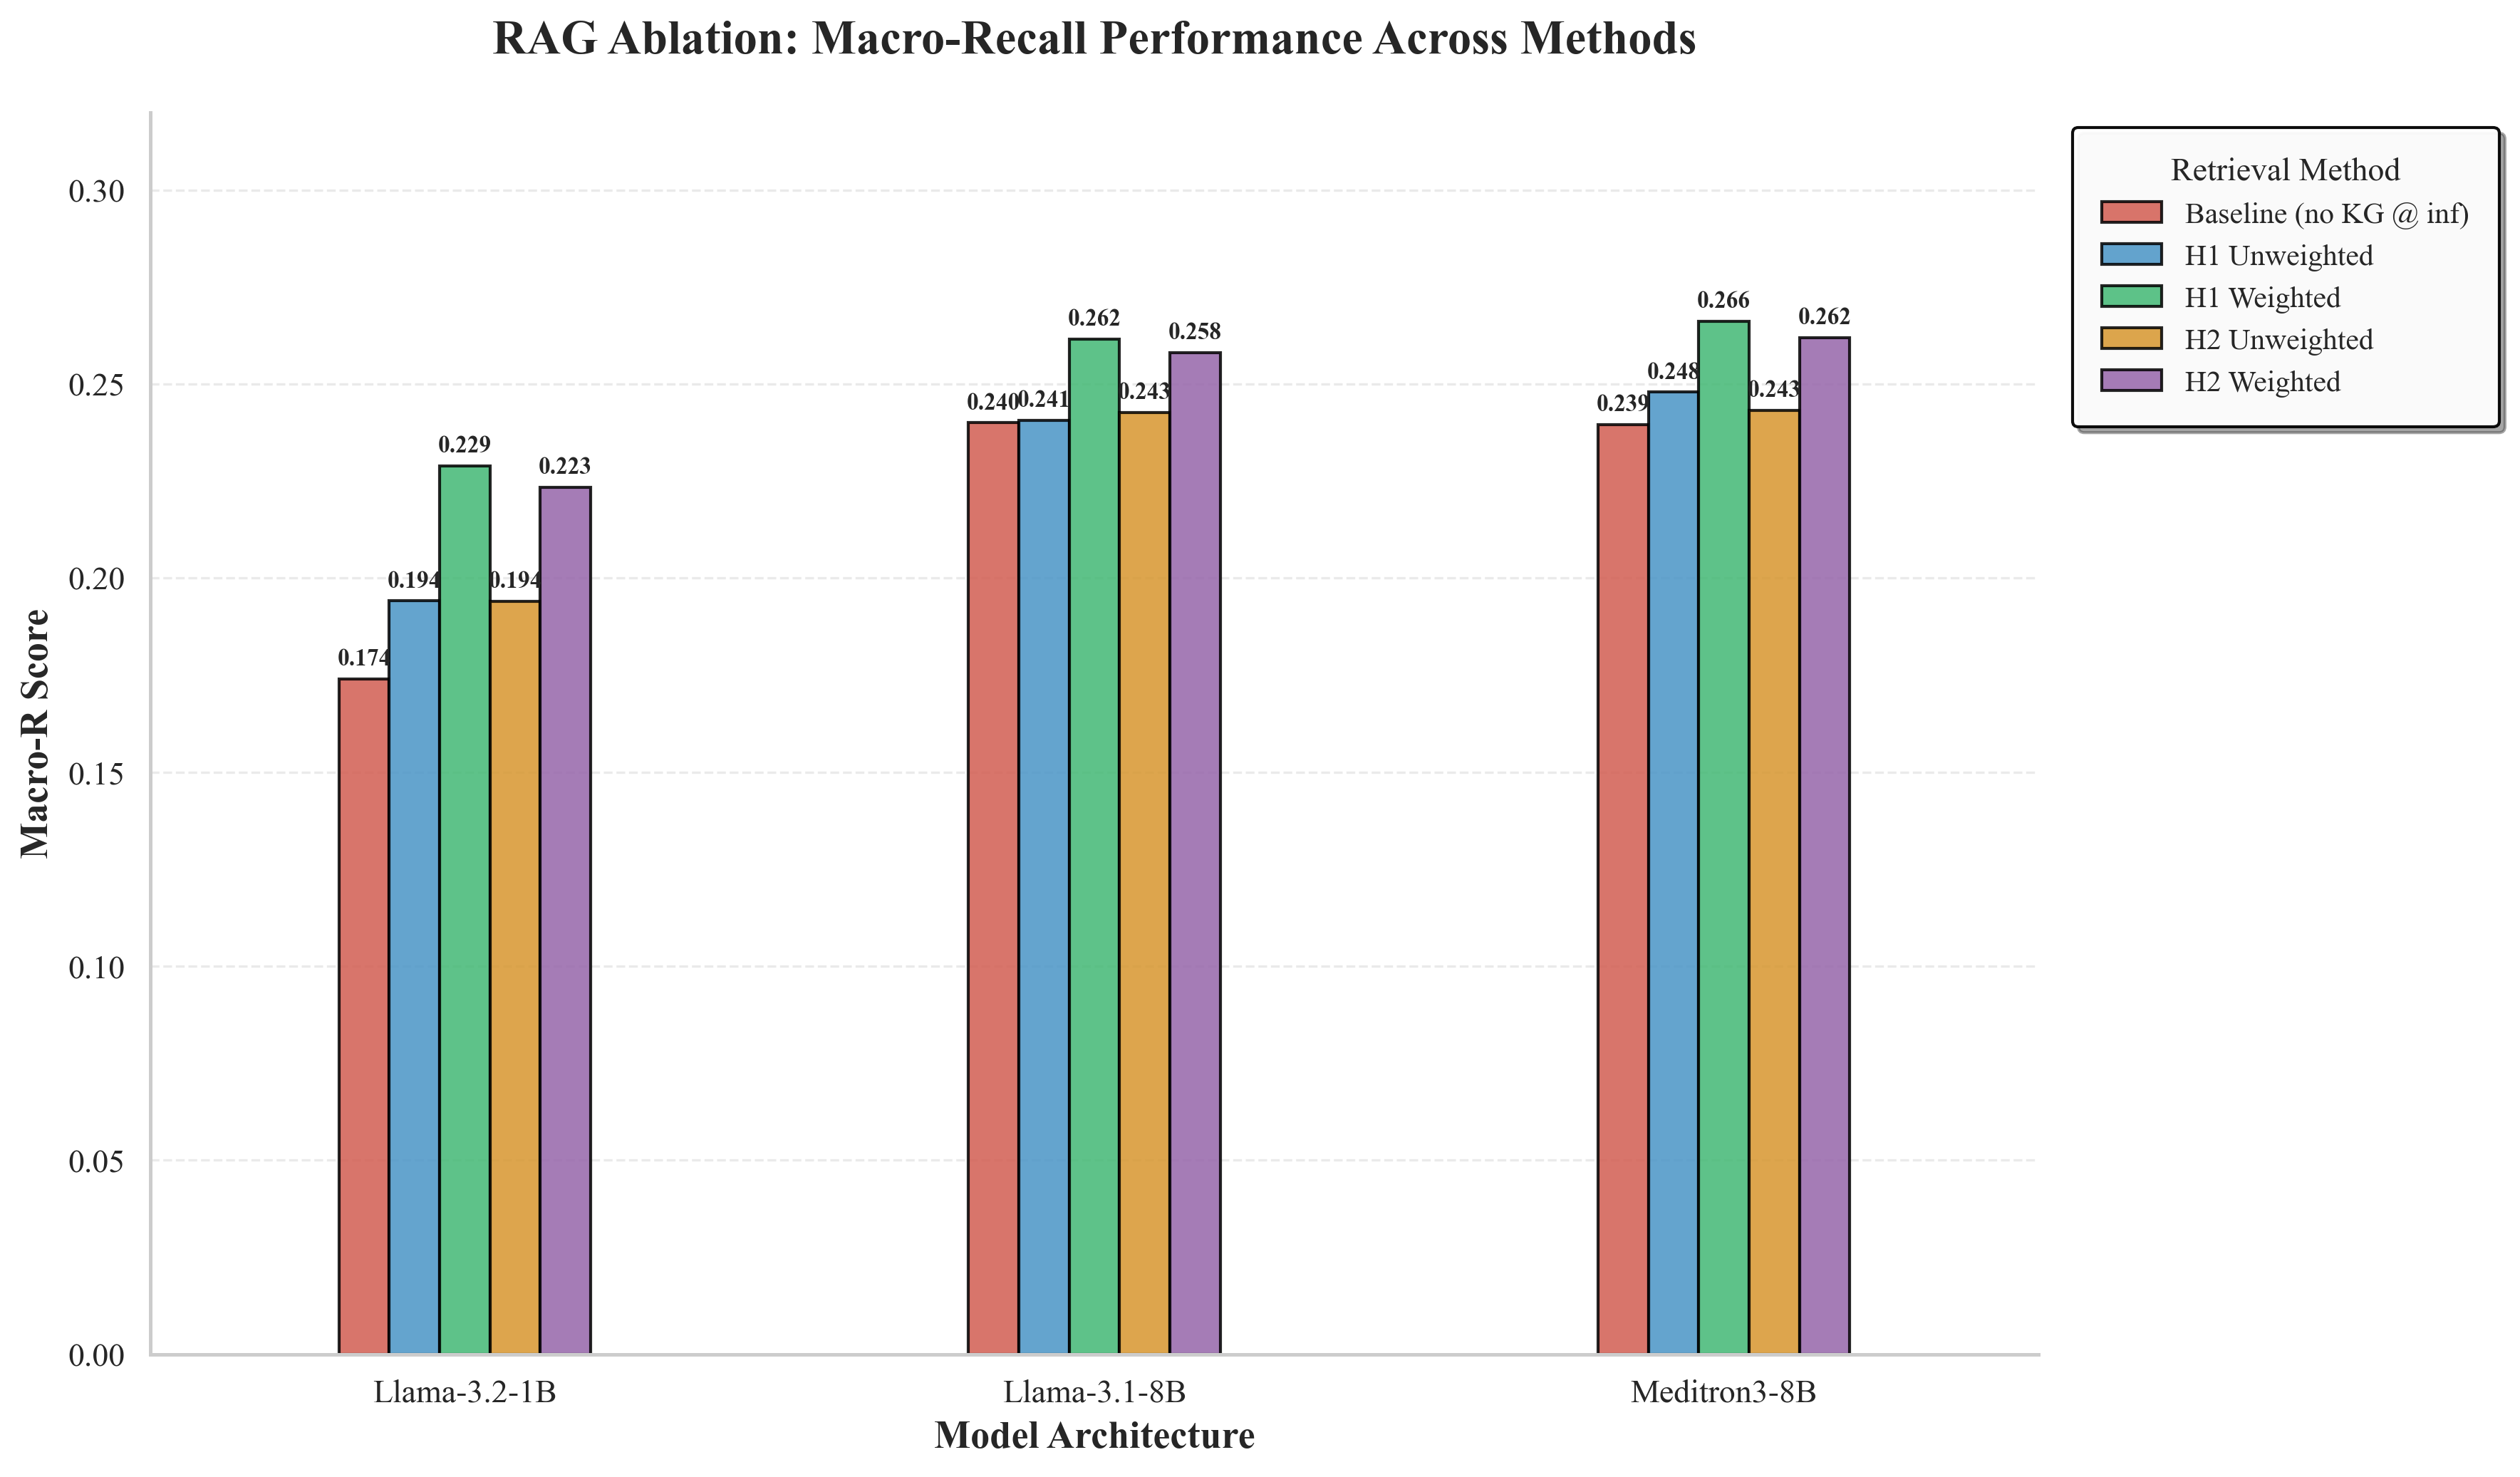
\includegraphics[width=\linewidth]{Images/h1vh2vbase/macro_recall.png}
        \caption{macro-recall}
        \label{fig:task1-bottom50-macroRecall}
    \end{subfigure}

    % third row
    \begin{subfigure}{0.48\textwidth}
        \centering
        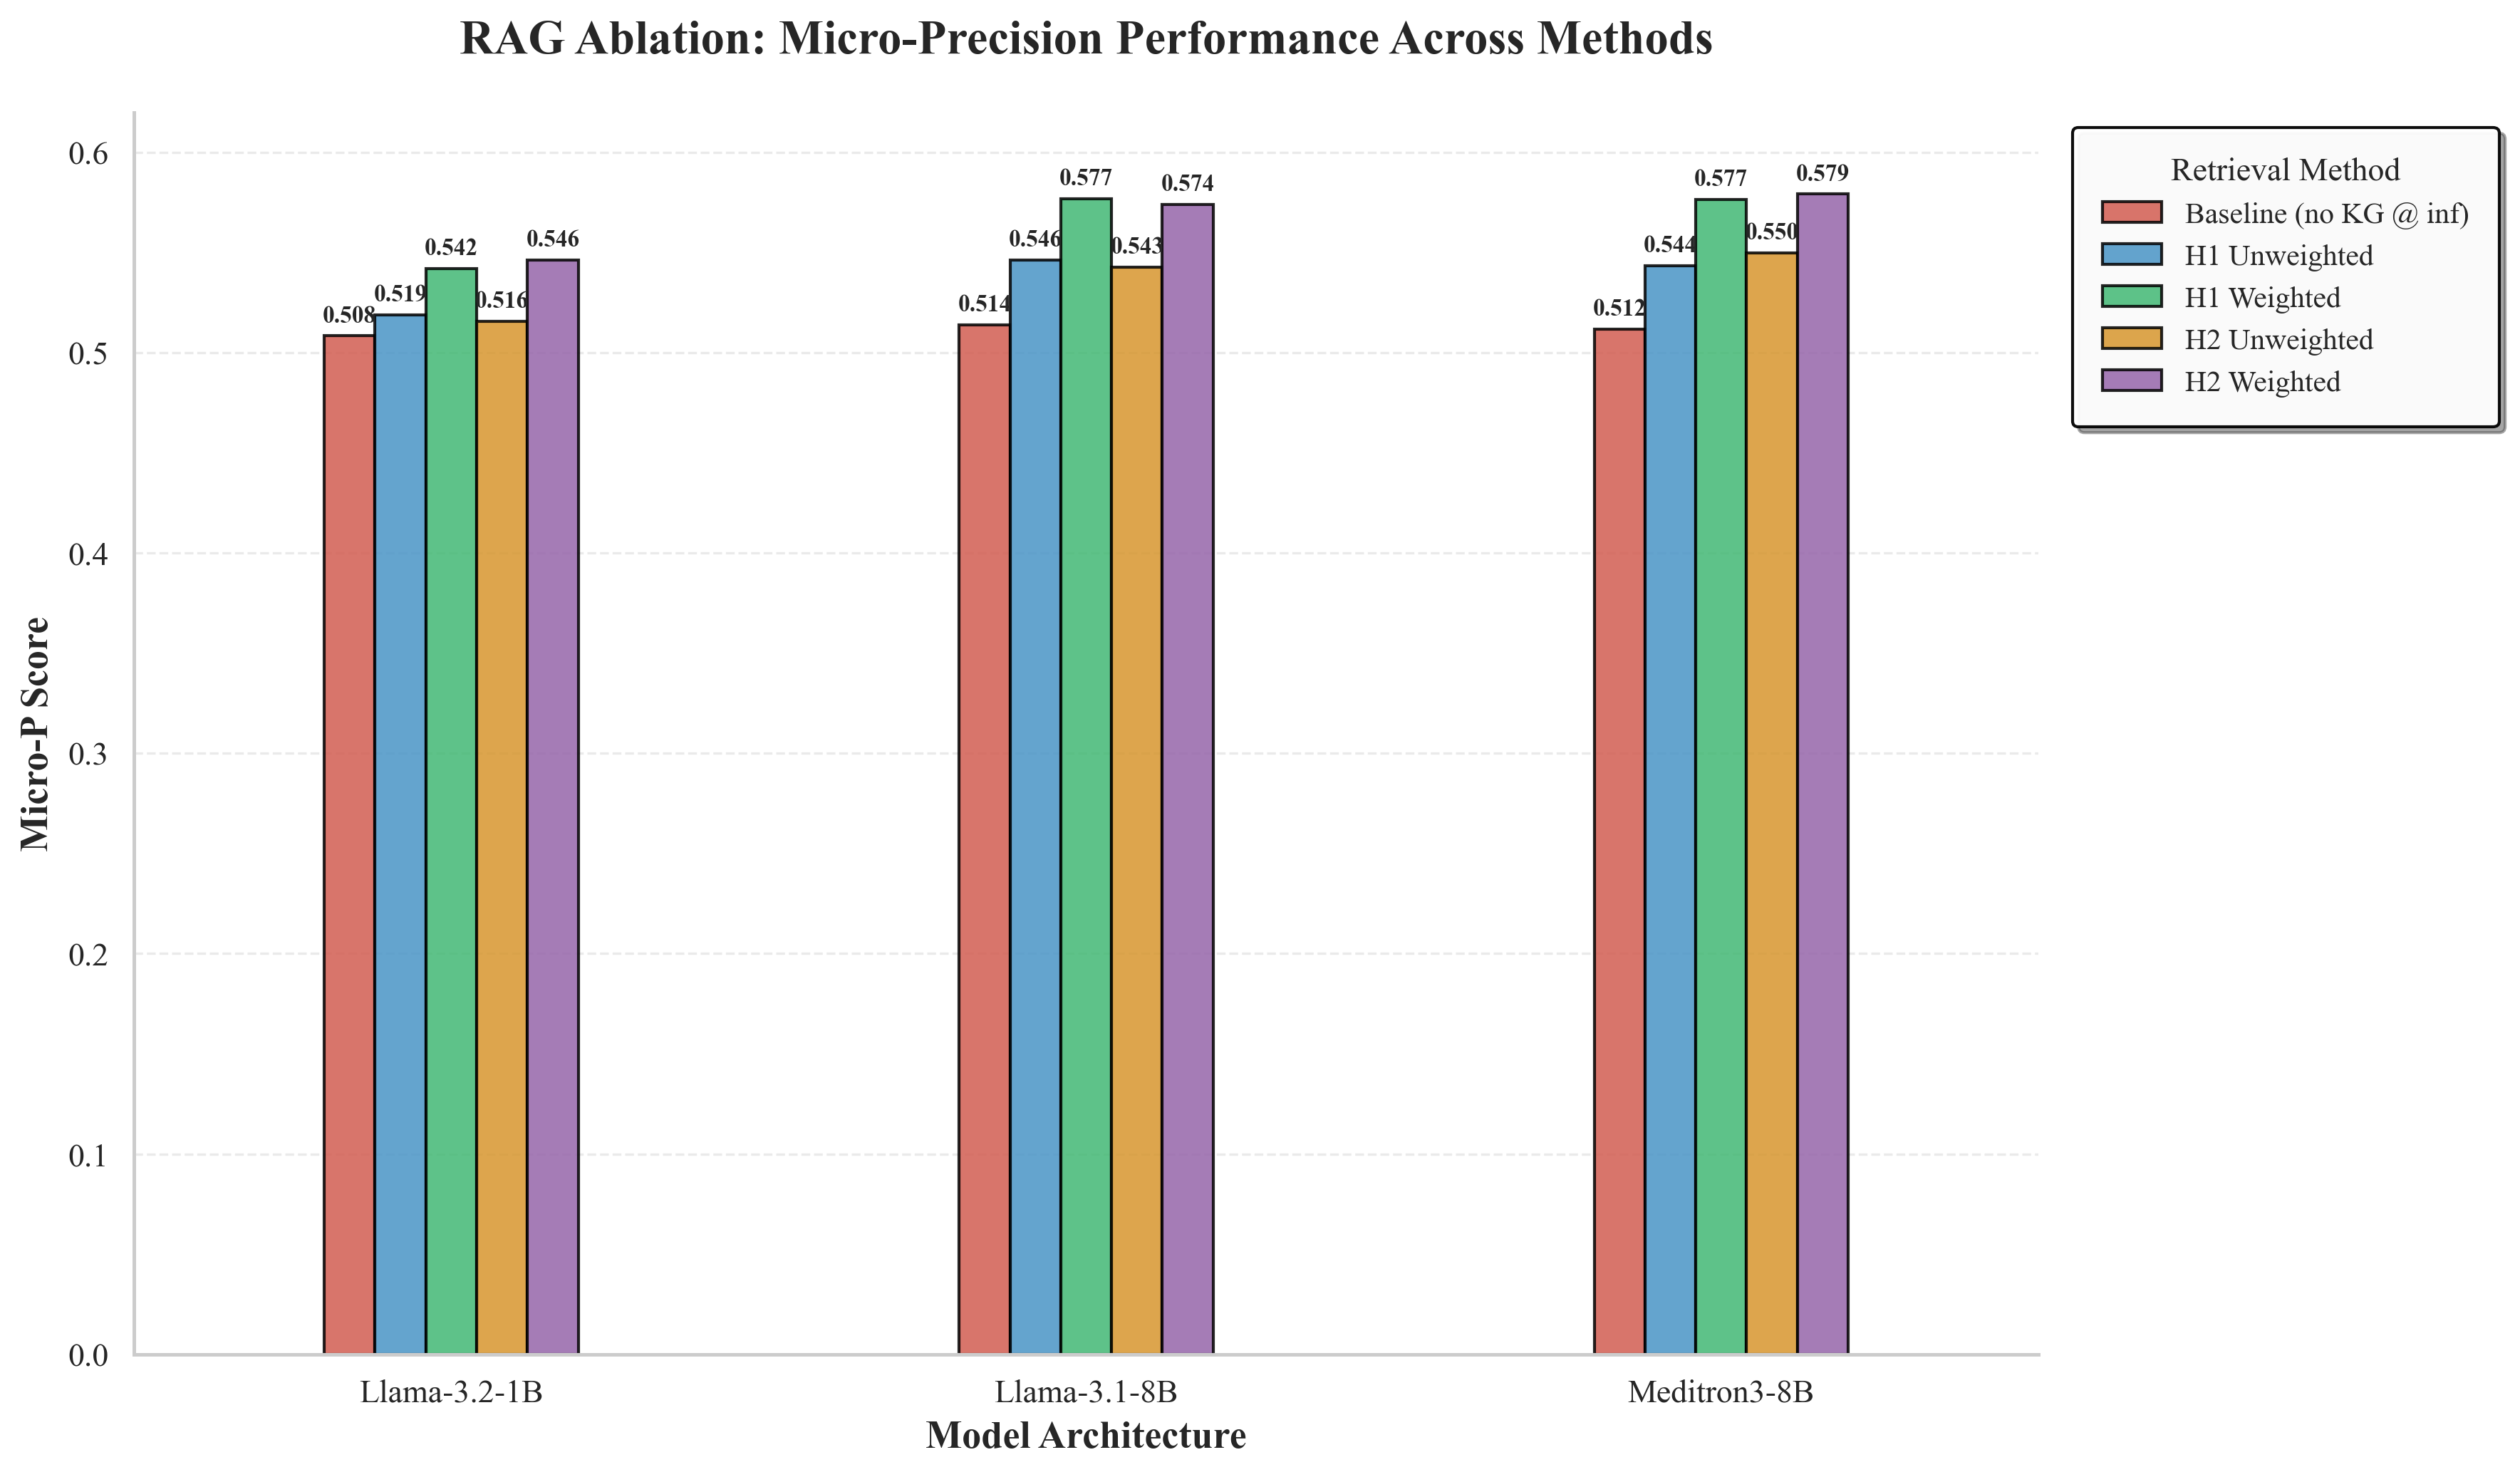
\includegraphics[width=\linewidth]{Images/h1vh2vbase/micro_precision.png}
        \caption{micro-precision}
        \label{fig:task1-bottom50-microPrecision}
    \end{subfigure}\hfill
    \begin{subfigure}{0.48\textwidth}
        \centering
        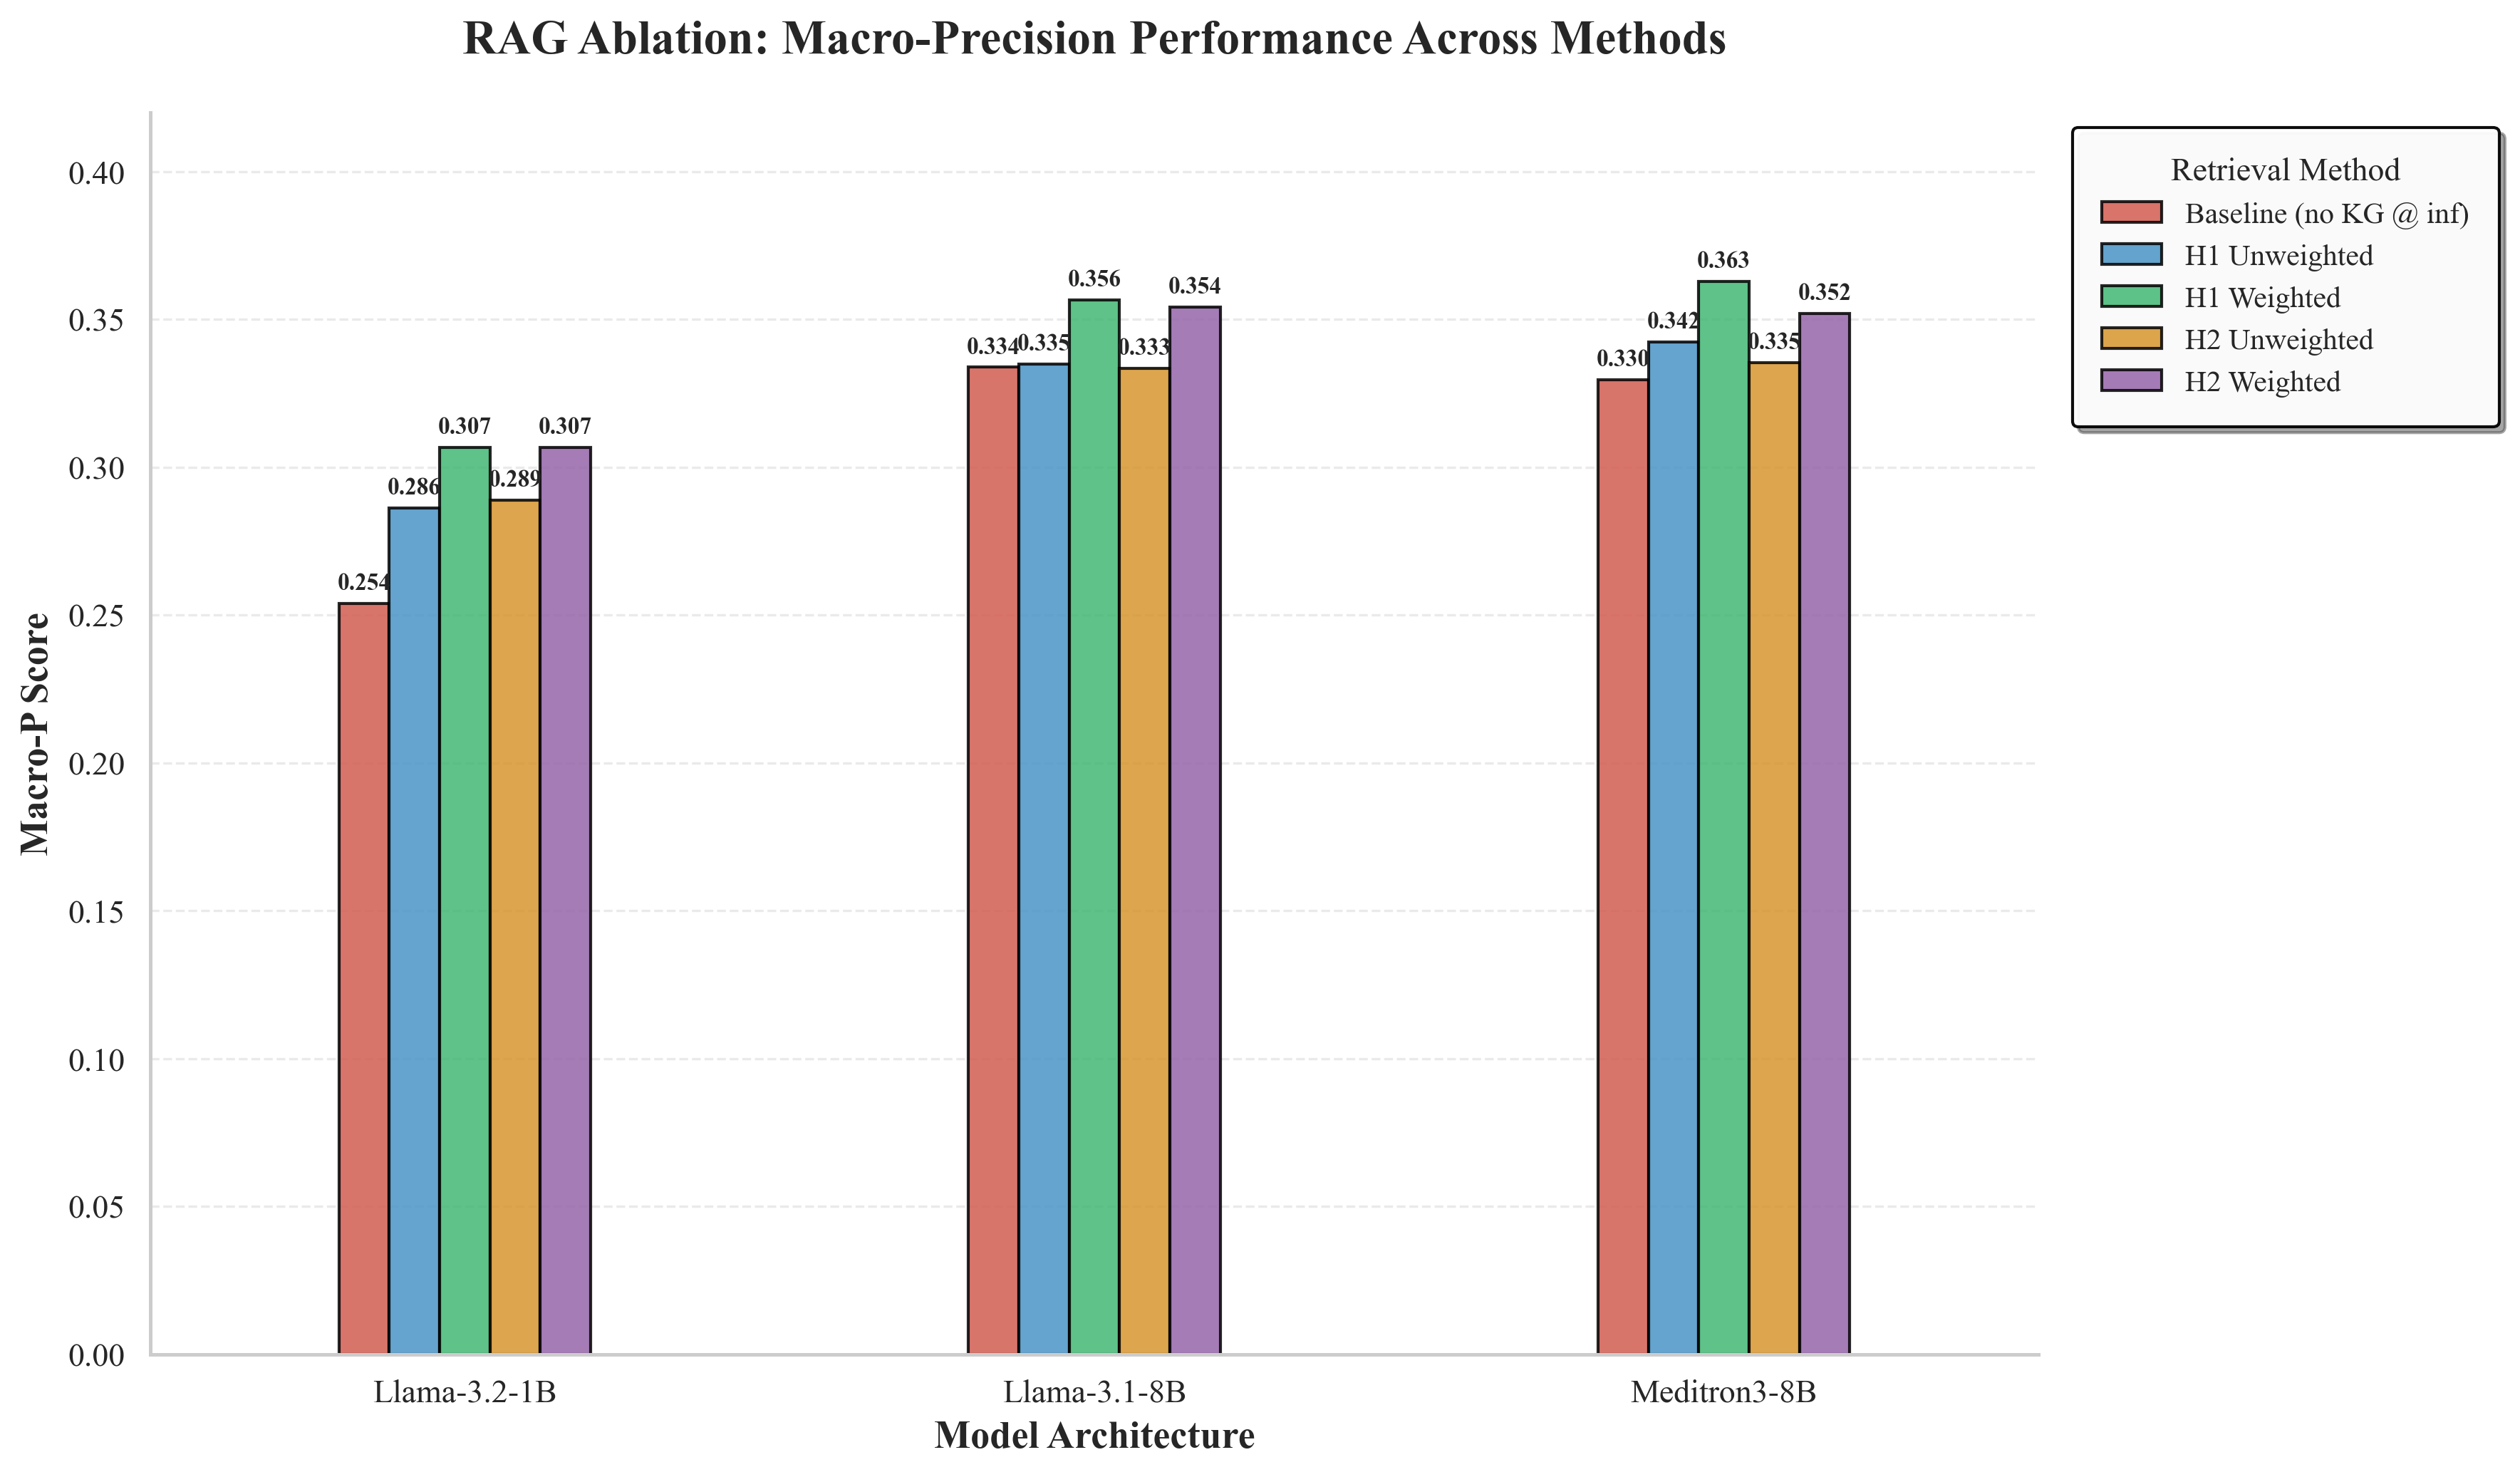
\includegraphics[width=\linewidth]{Images/h1vh2vbase/macro_precision.png}
        \caption{macro-precision}
        \label{fig:task1-bottom50-macroPrecision}
    \end{subfigure}

    \caption{Task~1: KG/RAG overall metrics: grouped bars (micro/macro P/R/F1) comparing Baseline vs.\ H1/H2 Unweighted vs.\ H1/H2 Weighted per backbone.}
    \label{fig:task1-rag-overall-plots}
\end{figure}

\paragraph{Hierarchical (parent-level) performance.}
Parent-level metrics also improve with KG-augmented fine-tuning, indicating that gains reflect better diagnostic-family alignment rather than superficial formatting.

\begin{table}[t]
\centering
\caption{Task~1 parent-level hierarchical metrics for KG-augmented (RAG) variants vs.\ Baseline TextGen (no KG at inference). Test set evaluation.}
\label{tab:task1-rag-parent}
\resizebox{\textwidth}{!}{
\begin{tabular}{llcccccc}
\toprule
\textbf{Model} & \textbf{Method} & \textbf{Micro-F1} & \textbf{Macro-F1} & \textbf{Micro-P} & \textbf{Macro-P} & \textbf{Micro-R} & \textbf{Macro-R} \\
\midrule
Llama-3.2-1B & H1 Unweighted & 0.5388 & 0.3174 & 0.6320 & 0.4162 & 0.4688 & 0.2874 \\
Llama-3.2-1B & H1 Weighted   & \textbf{0.5736} & \textbf{0.3412} & 0.6571 & 0.4351 & 0.5092 & 0.3155 \\
Llama-3.2-1B & H2 Unweighted & 0.5389 & 0.3174 & 0.6323 & 0.4163 & 0.4688 & 0.2874 \\
Llama-3.2-1B & H2 Weighted   & 0.5708 & 0.3401 & 0.6574 & 0.4388 & 0.5012 & 0.3110 \\
Llama-3.2-1B & Baseline TextGen (no KG @ inf) & 0.5396 & 0.3134 & 0.6248 & 0.4023 & 0.4761 & 0.2827 \\
\midrule
Llama-3.1-8B & H1 Unweighted & 0.5632 & 0.3617 & 0.6463 & 0.4622 & 0.4985 & 0.3333 \\
Llama-3.1-8B & H1 Weighted   & \textbf{0.5926} & \textbf{0.3788} & 0.6765 & 0.4757 & 0.5278 & 0.3507 \\
Llama-3.1-8B & H2 Unweighted & 0.5598 & 0.3663 & 0.6425 & 0.4621 & 0.4955 & 0.3373 \\
Llama-3.1-8B & H2 Weighted   & 0.5900 & 0.3789 & 0.6742 & 0.4817 & 0.5247 & 0.3505 \\
Llama-3.1-8B & Baseline TextGen (no KG @ inf) & 0.5545 & 0.3552 & 0.6202 & 0.4716 & 0.5033 & 0.3455 \\
\midrule
Meditron3-8B & H1 Unweighted & 0.5591 & 0.3720 & 0.6430 & 0.4691 & 0.4941 & 0.3480 \\
Meditron3-8B & H1 Weighted   & \textbf{0.5931} & \textbf{0.3902} & 0.6757 & 0.4907 & 0.5288 & 0.3655 \\
Meditron3-8B & H2 Unweighted & 0.5631 & 0.3622 & 0.6478 & 0.4475 & 0.4975 & 0.3380 \\
Meditron3-8B & H2 Weighted   & 0.5910 & 0.3835 & 0.6764 & 0.4742 & 0.5249 & 0.3597 \\
Meditron3-8B & Baseline TextGen (no KG @ inf) & 0.5456 & 0.3509 & 0.6138 & 0.4621 & 0.4939 & 0.3363 \\
\bottomrule
\end{tabular}}
\end{table}


\paragraph{Head-50 vs.\ Tail-50 effects (long-tail focus).}
Tables~\ref{tab:task1-rag-top50} and \ref{tab:task1-rag-tail50} decompose KG gains by frequency strata. Head-50 gains are moderate; the key scientific question is whether KG helps the \emph{tail} under sparse supervision and a strict 12-output constraint.

\begin{table}[t]
\centering
\caption{Task~1 Top-50 (Head-50) metrics for KG-augmented variants vs.\ Baseline TextGen (no KG at inference).}
\label{tab:task1-rag-top50}
\resizebox{\textwidth}{!}{
\begin{tabular}{llcccccc}
\toprule
\textbf{Model} & \textbf{Method} & \textbf{Micro-F1} & \textbf{Macro-F1} & \textbf{Micro-P} & \textbf{Macro-P} & \textbf{Micro-R} & \textbf{Macro-R} \\
\midrule
Llama-3.2-1B & H1 Unweighted & 0.6009 & 0.5473 & 0.6308 & 0.6134 & 0.5729 & 0.5110 \\
Llama-3.2-1B & H1 Weighted   & \textbf{0.6375} & \textbf{0.5839} & 0.6590 & 0.6391 & 0.6173 & 0.5563 \\
Llama-3.2-1B & H2 Unweighted & 0.6005 & 0.5474 & 0.6337 & 0.6159 & 0.5700 & 0.5117 \\
Llama-3.2-1B & H2 Weighted   & 0.6334 & 0.5799 & 0.6637 & 0.6451 & 0.6055 & 0.5451 \\
Llama-3.2-1B & Baseline TextGen (no KG @ inf) & 0.6011 & 0.5486 & 0.6413 & 0.6528 & 0.5655 & 0.5136 \\
\midrule
Llama-3.1-8B & H1 Unweighted & 0.6259 & 0.5683 & 0.6513 & 0.6323 & 0.6017 & 0.5387 \\
Llama-3.1-8B & H1 Weighted   & \textbf{0.6535} & \textbf{0.5952} & 0.6780 & 0.6608 & 0.6308 & 0.5669 \\
Llama-3.1-8B & H2 Unweighted & 0.6209 & 0.5635 & 0.6468 & 0.6282 & 0.5974 & 0.5340 \\
Llama-3.1-8B & H2 Weighted   & 0.6500 & 0.5927 & 0.6720 & 0.6562 & 0.6294 & 0.5652 \\
Llama-3.1-8B & Baseline TextGen (no KG @ inf) & 0.5984 & 0.5443 & 0.6322 & 0.6280 & 0.5680 & 0.5195 \\
\midrule
Meditron3-8B & H1 Unweighted & 0.6162 & 0.5596 & 0.6430 & 0.6231 & 0.5914 & 0.5288 \\
Meditron3-8B & H1 Weighted   & \textbf{0.6529} & \textbf{0.5954} & 0.6791 & 0.6611 & 0.6288 & 0.5648 \\
Meditron3-8B & H2 Unweighted & 0.6238 & 0.5673 & 0.6523 & 0.6339 & 0.5976 & 0.5352 \\
Meditron3-8B & H2 Weighted   & 0.6529 & 0.5946 & 0.6826 & 0.6624 & 0.6257 & 0.5636 \\
Meditron3-8B & Baseline TextGen (no KG @ inf) & 0.5879 & 0.5276 & 0.6298 & 0.6310 & 0.5514 & 0.4977 \\
\bottomrule
\end{tabular}}
\end{table}

\begin{table}[t]
\centering
\caption{Task~1 Bottom-50 (Tail-50) metrics for KG-augmented variants vs.\ Baseline TextGen (no KG at inference).}
\label{tab:task1-rag-tail50}
\resizebox{\textwidth}{!}{
\begin{tabular}{llcccccc}
\toprule
\textbf{Model} & \textbf{Method} & \textbf{Micro-F1} & \textbf{Macro-F1} & \textbf{Micro-P} & \textbf{Macro-P} & \textbf{Micro-R} & \textbf{Macro-R} \\
\midrule
Llama-3.2-1B & H1 Unweighted & 0.1304 & 0.0427 & 0.3333 & 0.0345 & 0.0811 & 0.0575 \\
Llama-3.2-1B & H1 Weighted   & 0.1509 & 0.0740 & 0.4100 & 0.0880 & 0.0950 & 0.0695 \\
Llama-3.2-1B & H2 Unweighted & 0.1702 & 0.0747 & 0.4000 & 0.0977 & 0.1081 & 0.0747 \\
Llama-3.2-1B & H2 Weighted   & \textbf{0.1841} & \textbf{0.0865} & 0.4200 & 0.1050 & 0.1150 & 0.0805 \\
Llama-3.2-1B & Baseline TextGen (no KG @ inf) & 0.1429 & 0.0761 & 0.3333 & 0.0880 & 0.0950 & 0.0695 \\
\midrule
Llama-3.1-8B & H1 Unweighted & 0.1364 & 0.0747 & 0.4286 & 0.1034 & 0.0811 & 0.0632 \\
Llama-3.1-8B & H1 Weighted   & 0.1689 & 0.1140 & 0.3600 & 0.1450 & 0.1100 & 0.1010 \\
Llama-3.1-8B & H2 Unweighted & 0.1304 & 0.0747 & 0.3333 & 0.1034 & 0.0811 & 0.0632 \\
Llama-3.1-8B & H2 Weighted   & \textbf{0.1820} & \textbf{0.1215} & 0.3500 & 0.1520 & 0.1220 & 0.1085 \\
Llama-3.1-8B & Baseline TextGen (no KG @ inf) & 0.1250 & 0.0719 & 0.3000 & 0.0862 & 0.0811 & 0.0632 \\
\midrule
Meditron3-8B & H1 Unweighted & 0.1739 & 0.0920 & 0.4444 & 0.1379 & 0.1081 & 0.0747 \\
Meditron3-8B & H1 Weighted   & \textbf{0.1915} & \textbf{0.1220} & 0.4100 & 0.1600 & 0.1250 & 0.1080 \\
Meditron3-8B & H2 Unweighted & 0.1778 & 0.1092 & 0.5000 & 0.1379 & 0.1081 & 0.0977 \\
Meditron3-8B & H2 Weighted   & 0.1890 & 0.1185 & 0.4600 & 0.1550 & 0.1200 & 0.1060 \\
Meditron3-8B & Baseline TextGen (no KG @ inf) & 0.1518 & 0.0885 & 0.5400 & 0.1157 & 0.1022 & 0.0716 \\
\bottomrule
\end{tabular}}
\end{table}

\begin{figure}[t]
    \centering
    % first row
    \begin{subfigure}{0.5\textwidth}
        \centering
        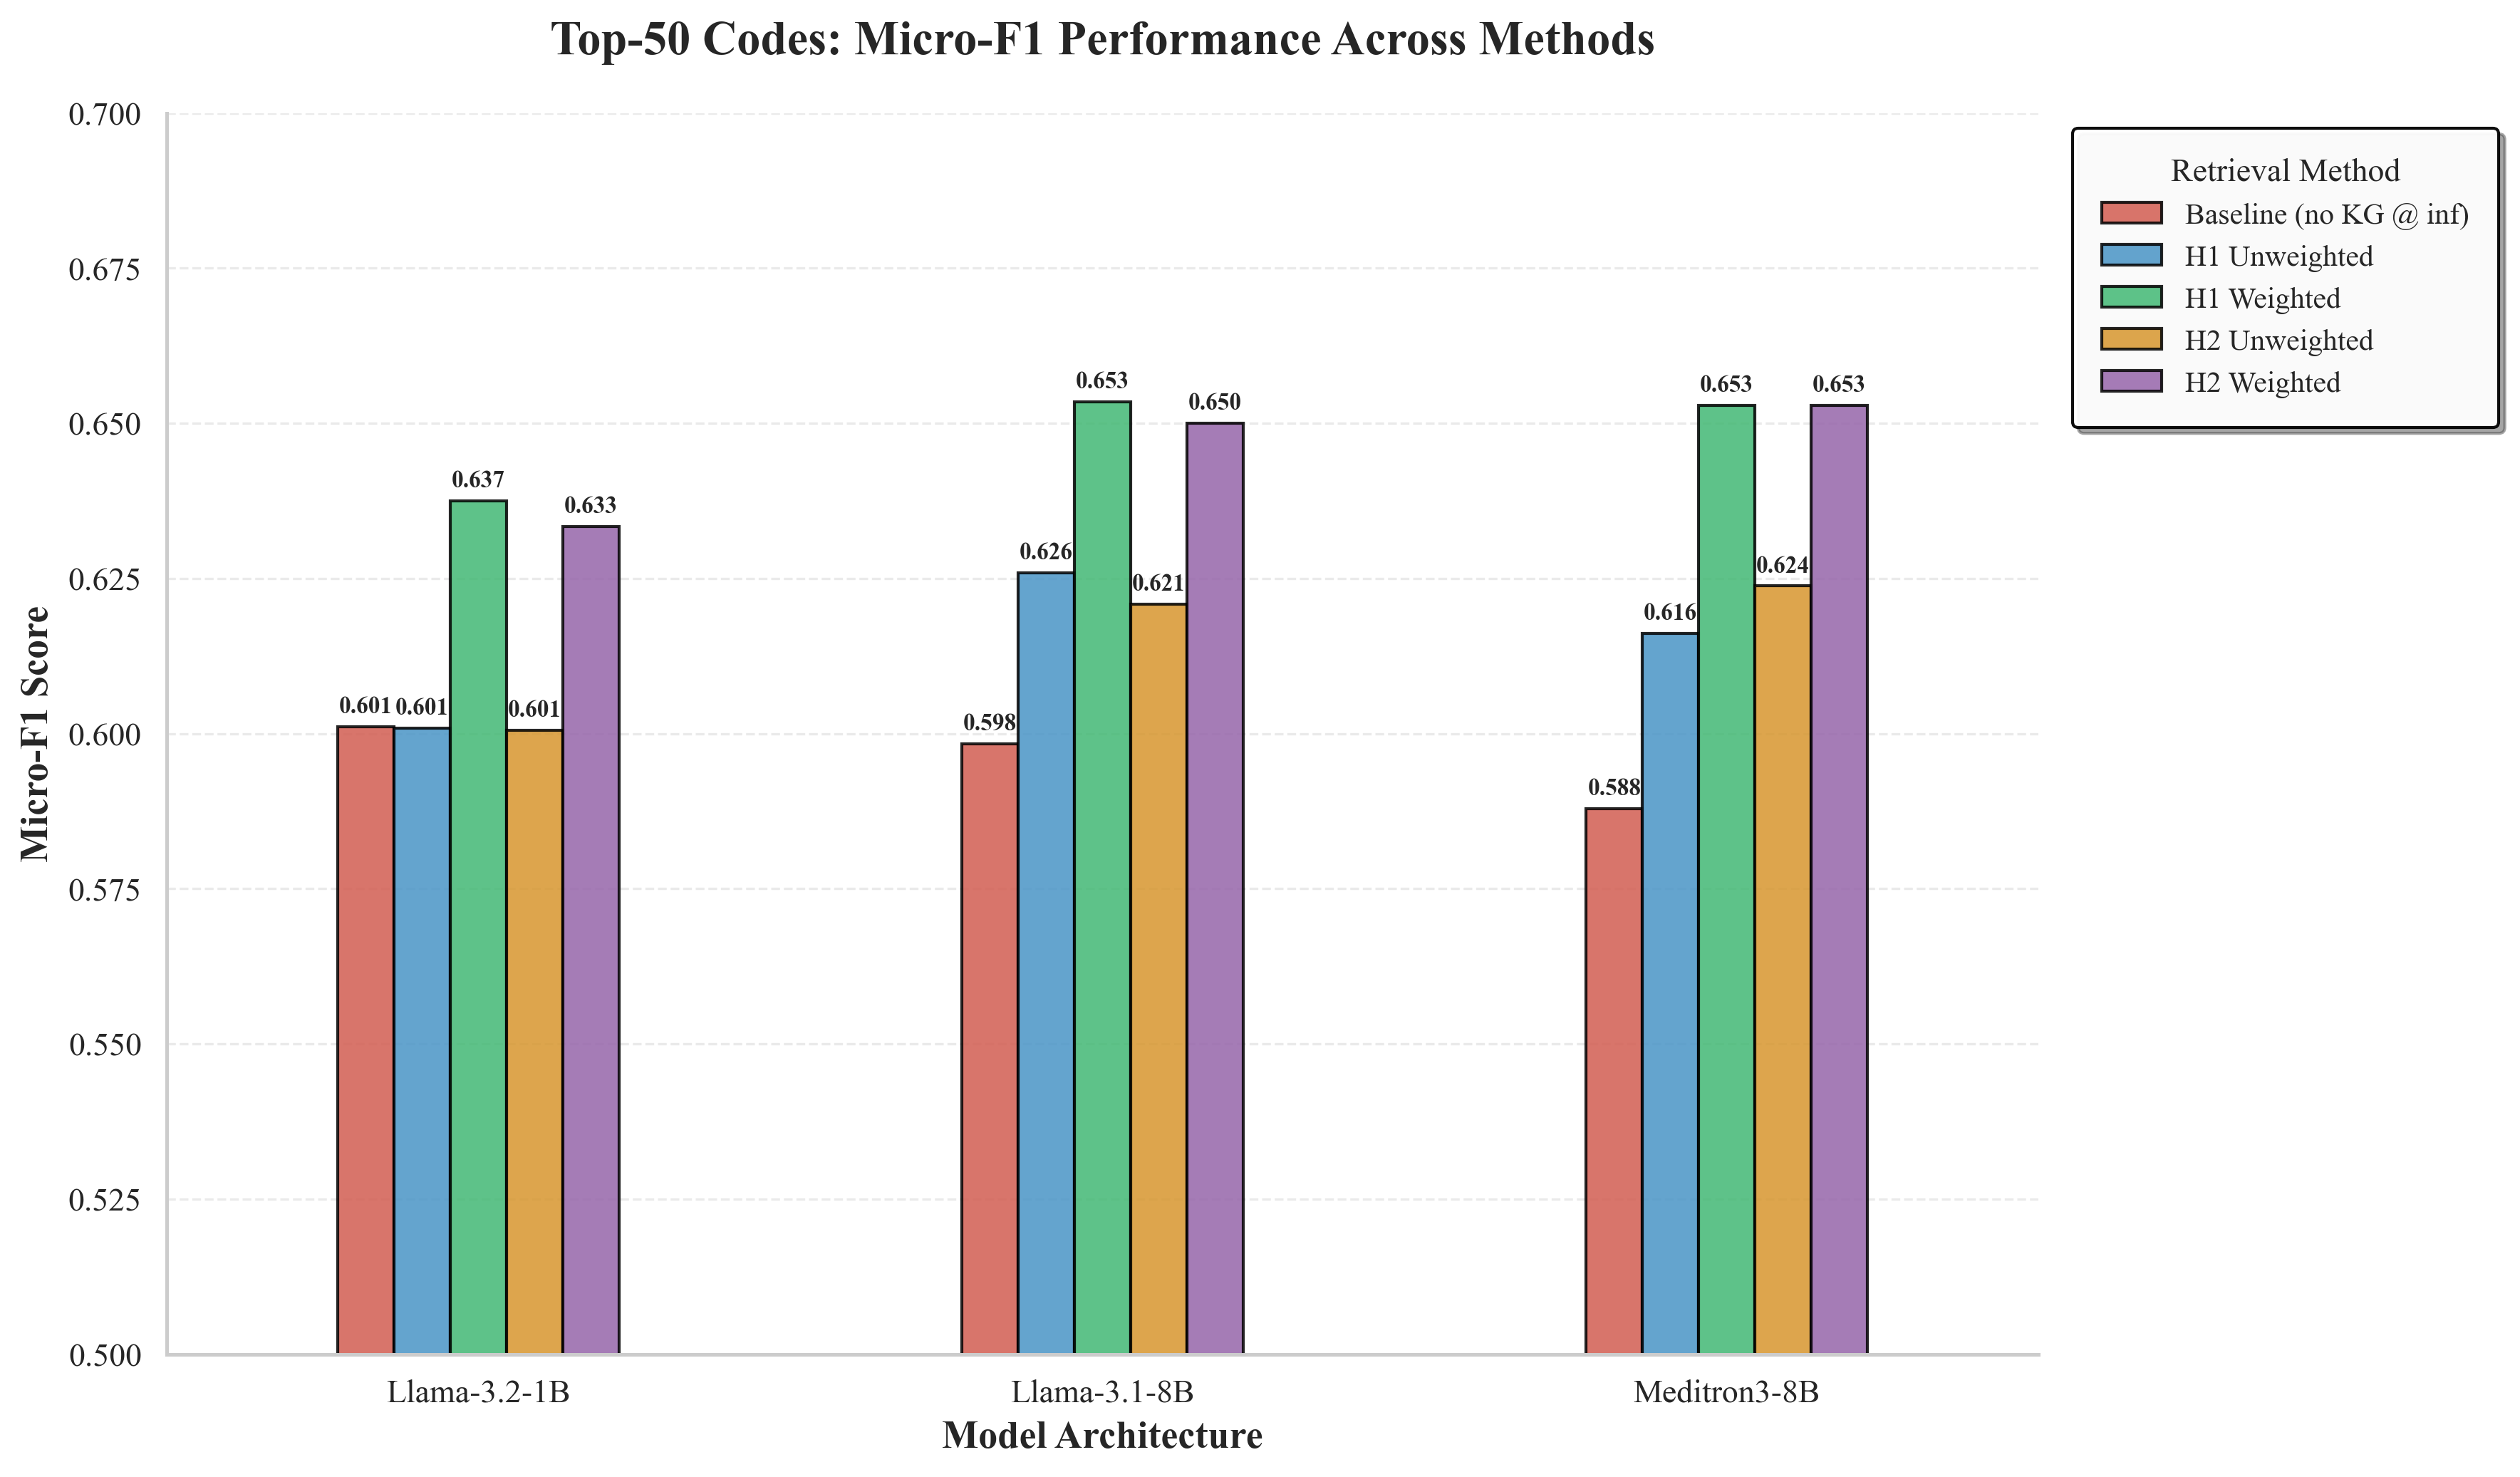
\includegraphics[width=\linewidth]{Images/h1vh2vbase/new/top50_micro_f1.png}
        \caption{Top50 micro-F1}
        \label{fig:task1-h1vh2vbase-top50microF1}
    \end{subfigure}\hfill
    \begin{subfigure}{0.5\textwidth}
        \centering
        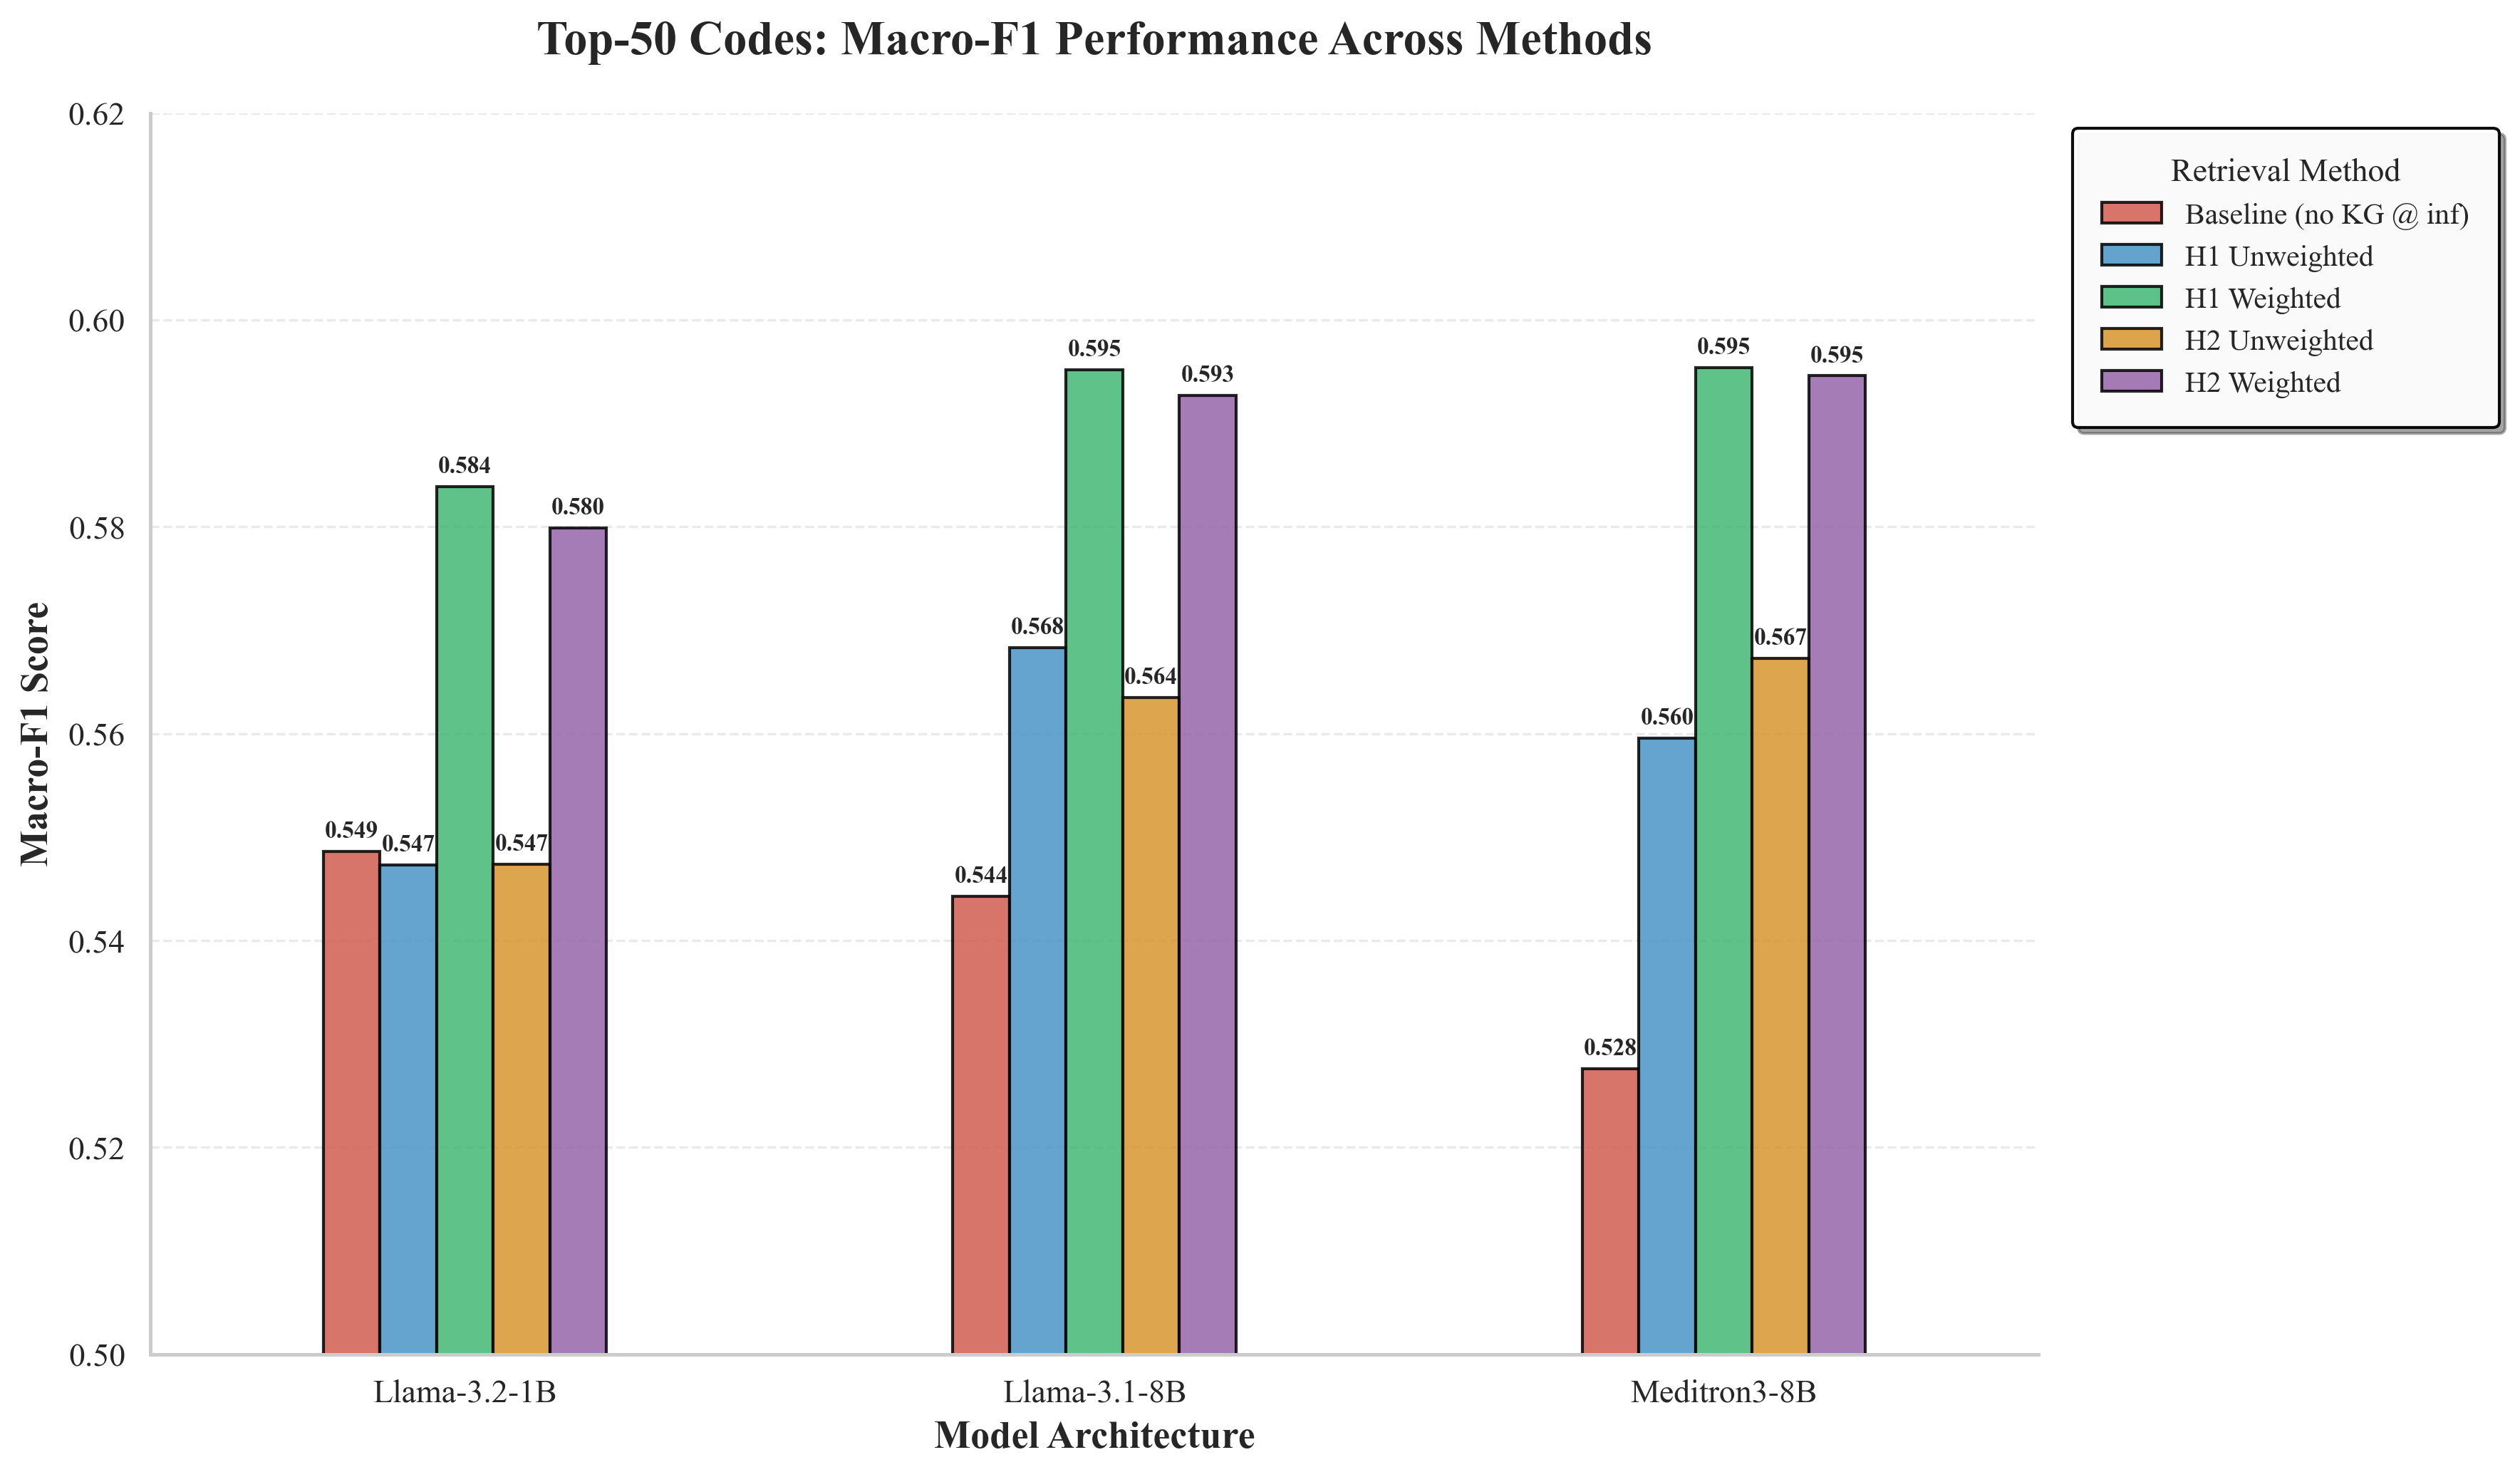
\includegraphics[width=\linewidth]{Images/h1vh2vbase/new/top50_macro_f1.png}
        \caption{Top50 macro-F1}
        \label{fig:task1-h1vh2vbase-top50macroF1}
    \end{subfigure}

    \vspace{0.3cm}

    % second row
    \begin{subfigure}{0.5\textwidth}
        \centering
        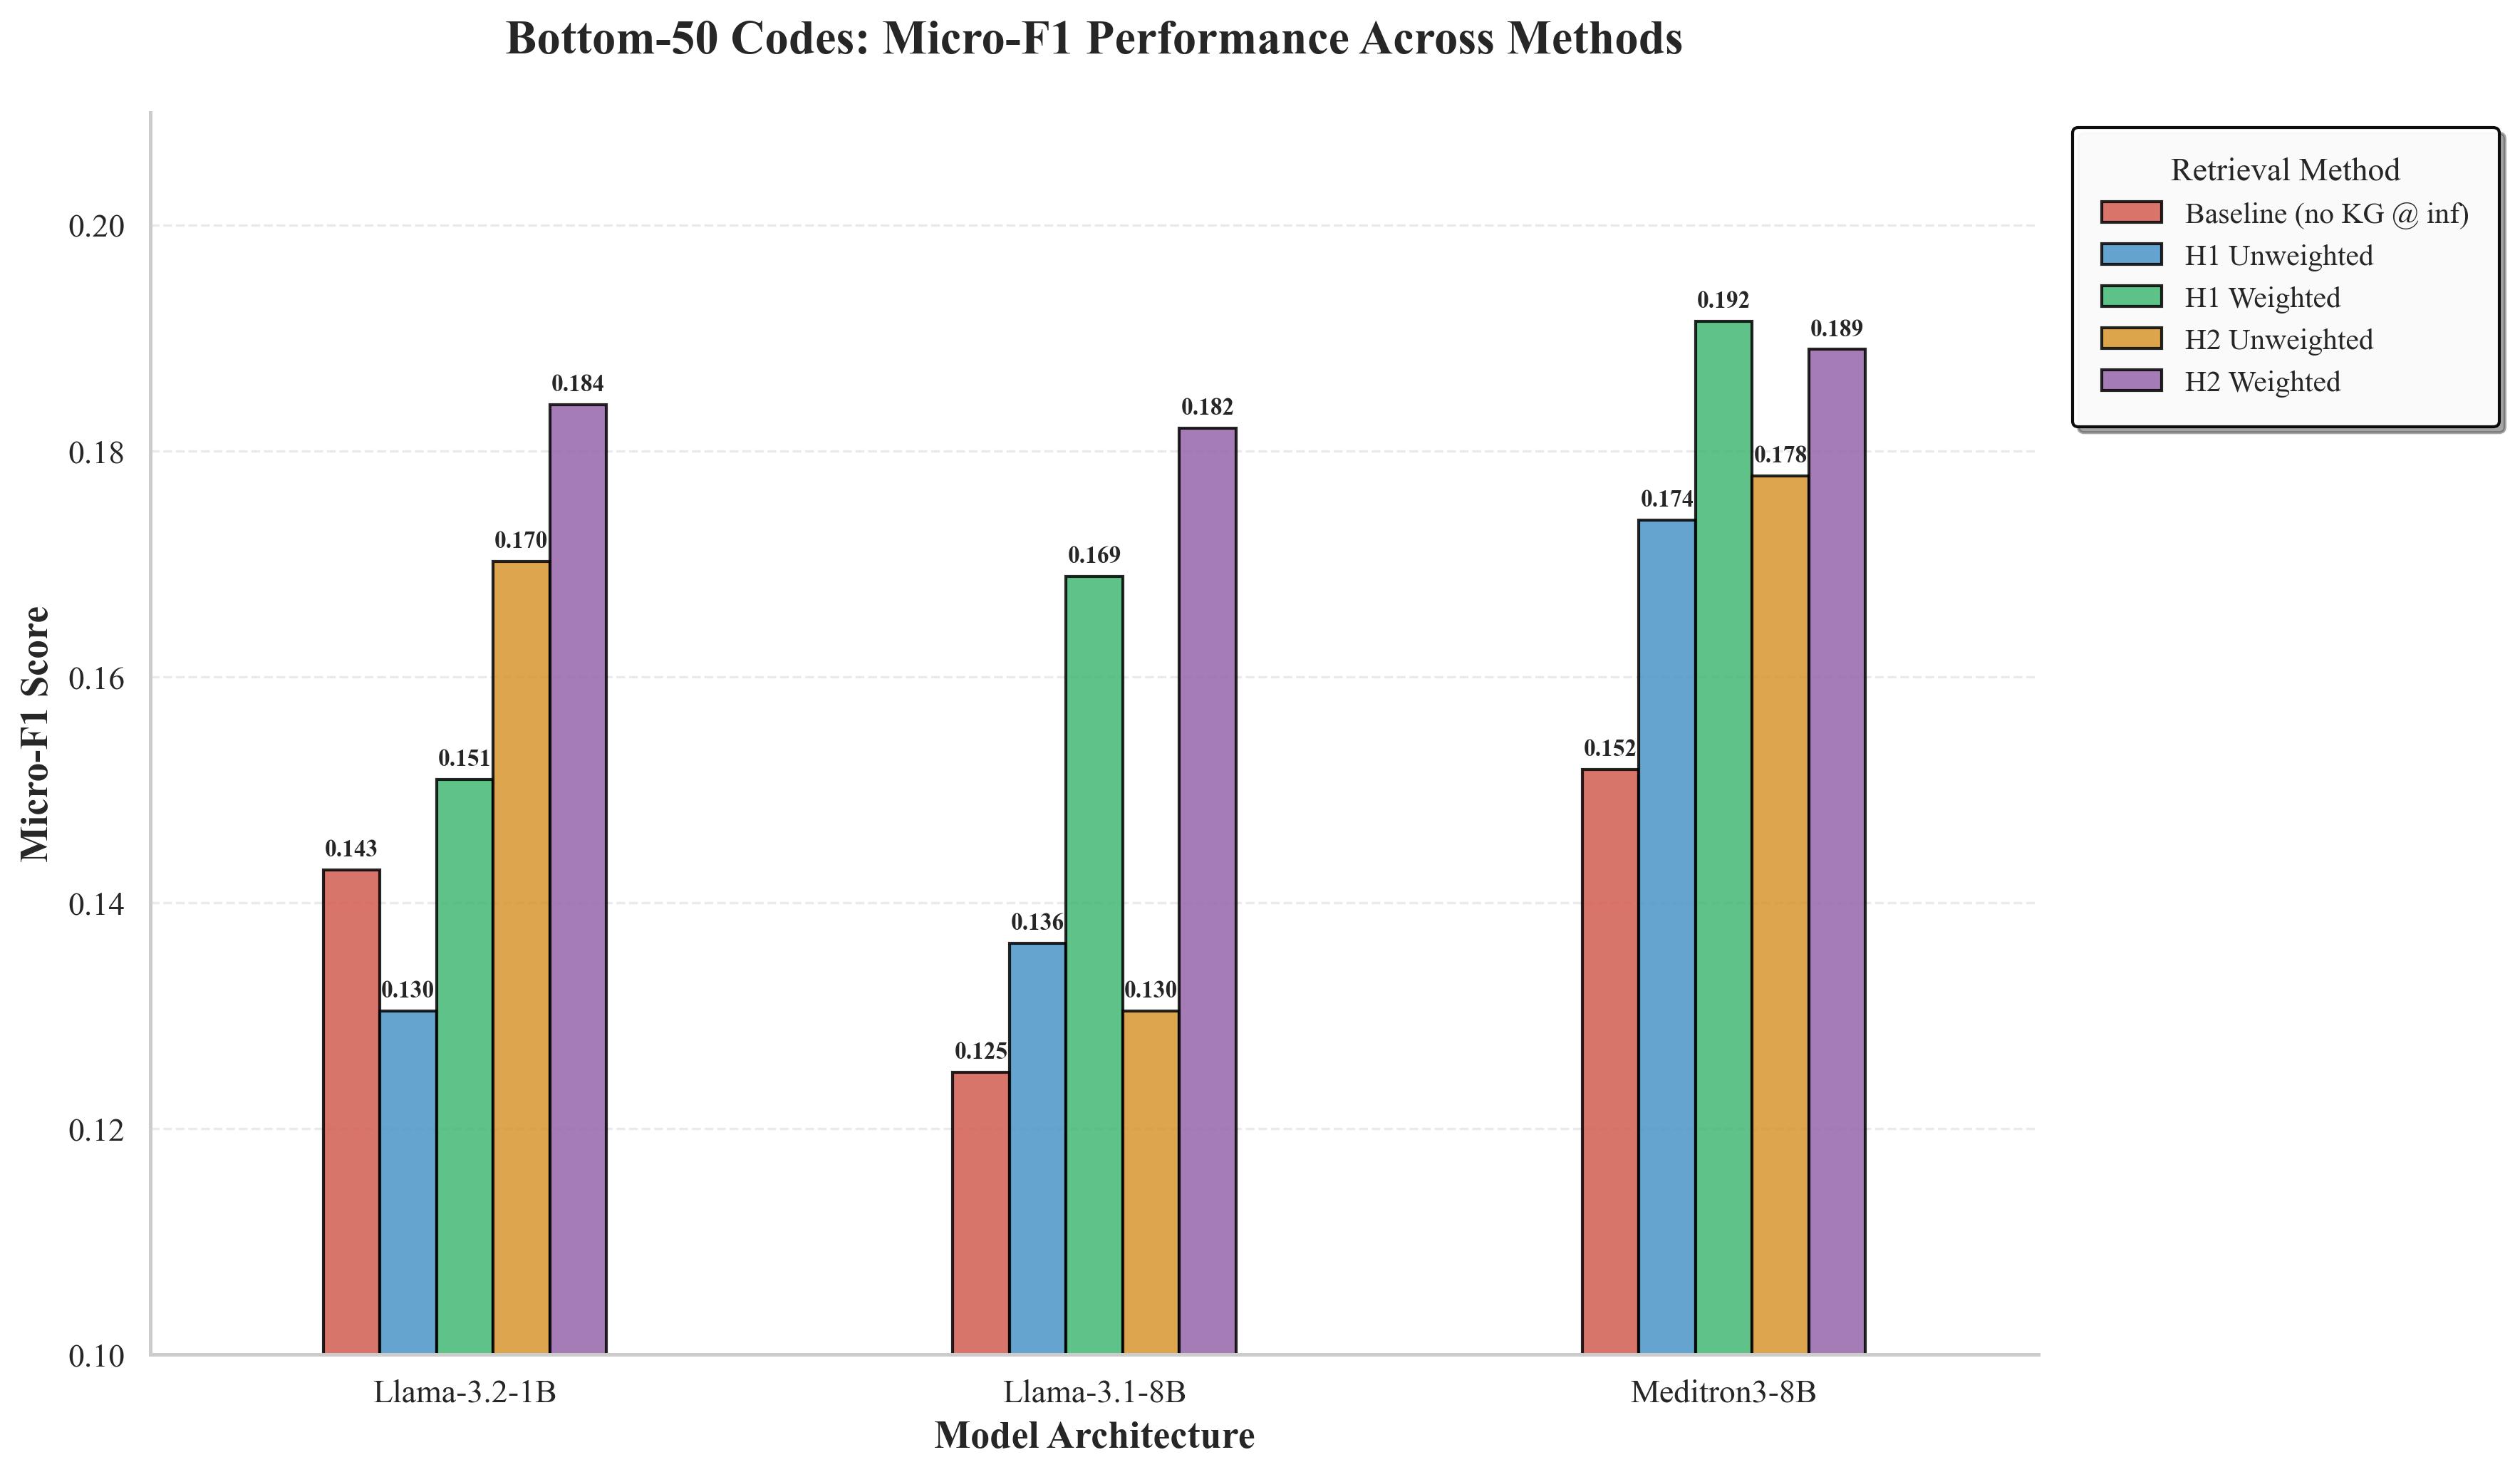
\includegraphics[width=\linewidth]{Images/h1vh2vbase/new/bottom50_micro_f1.png}
        \caption{Bottom50 micro-F1}
        \label{fig:task1-bottom50-microF1}
    \end{subfigure}\hfill
    \begin{subfigure}{0.5\textwidth}
        \centering
        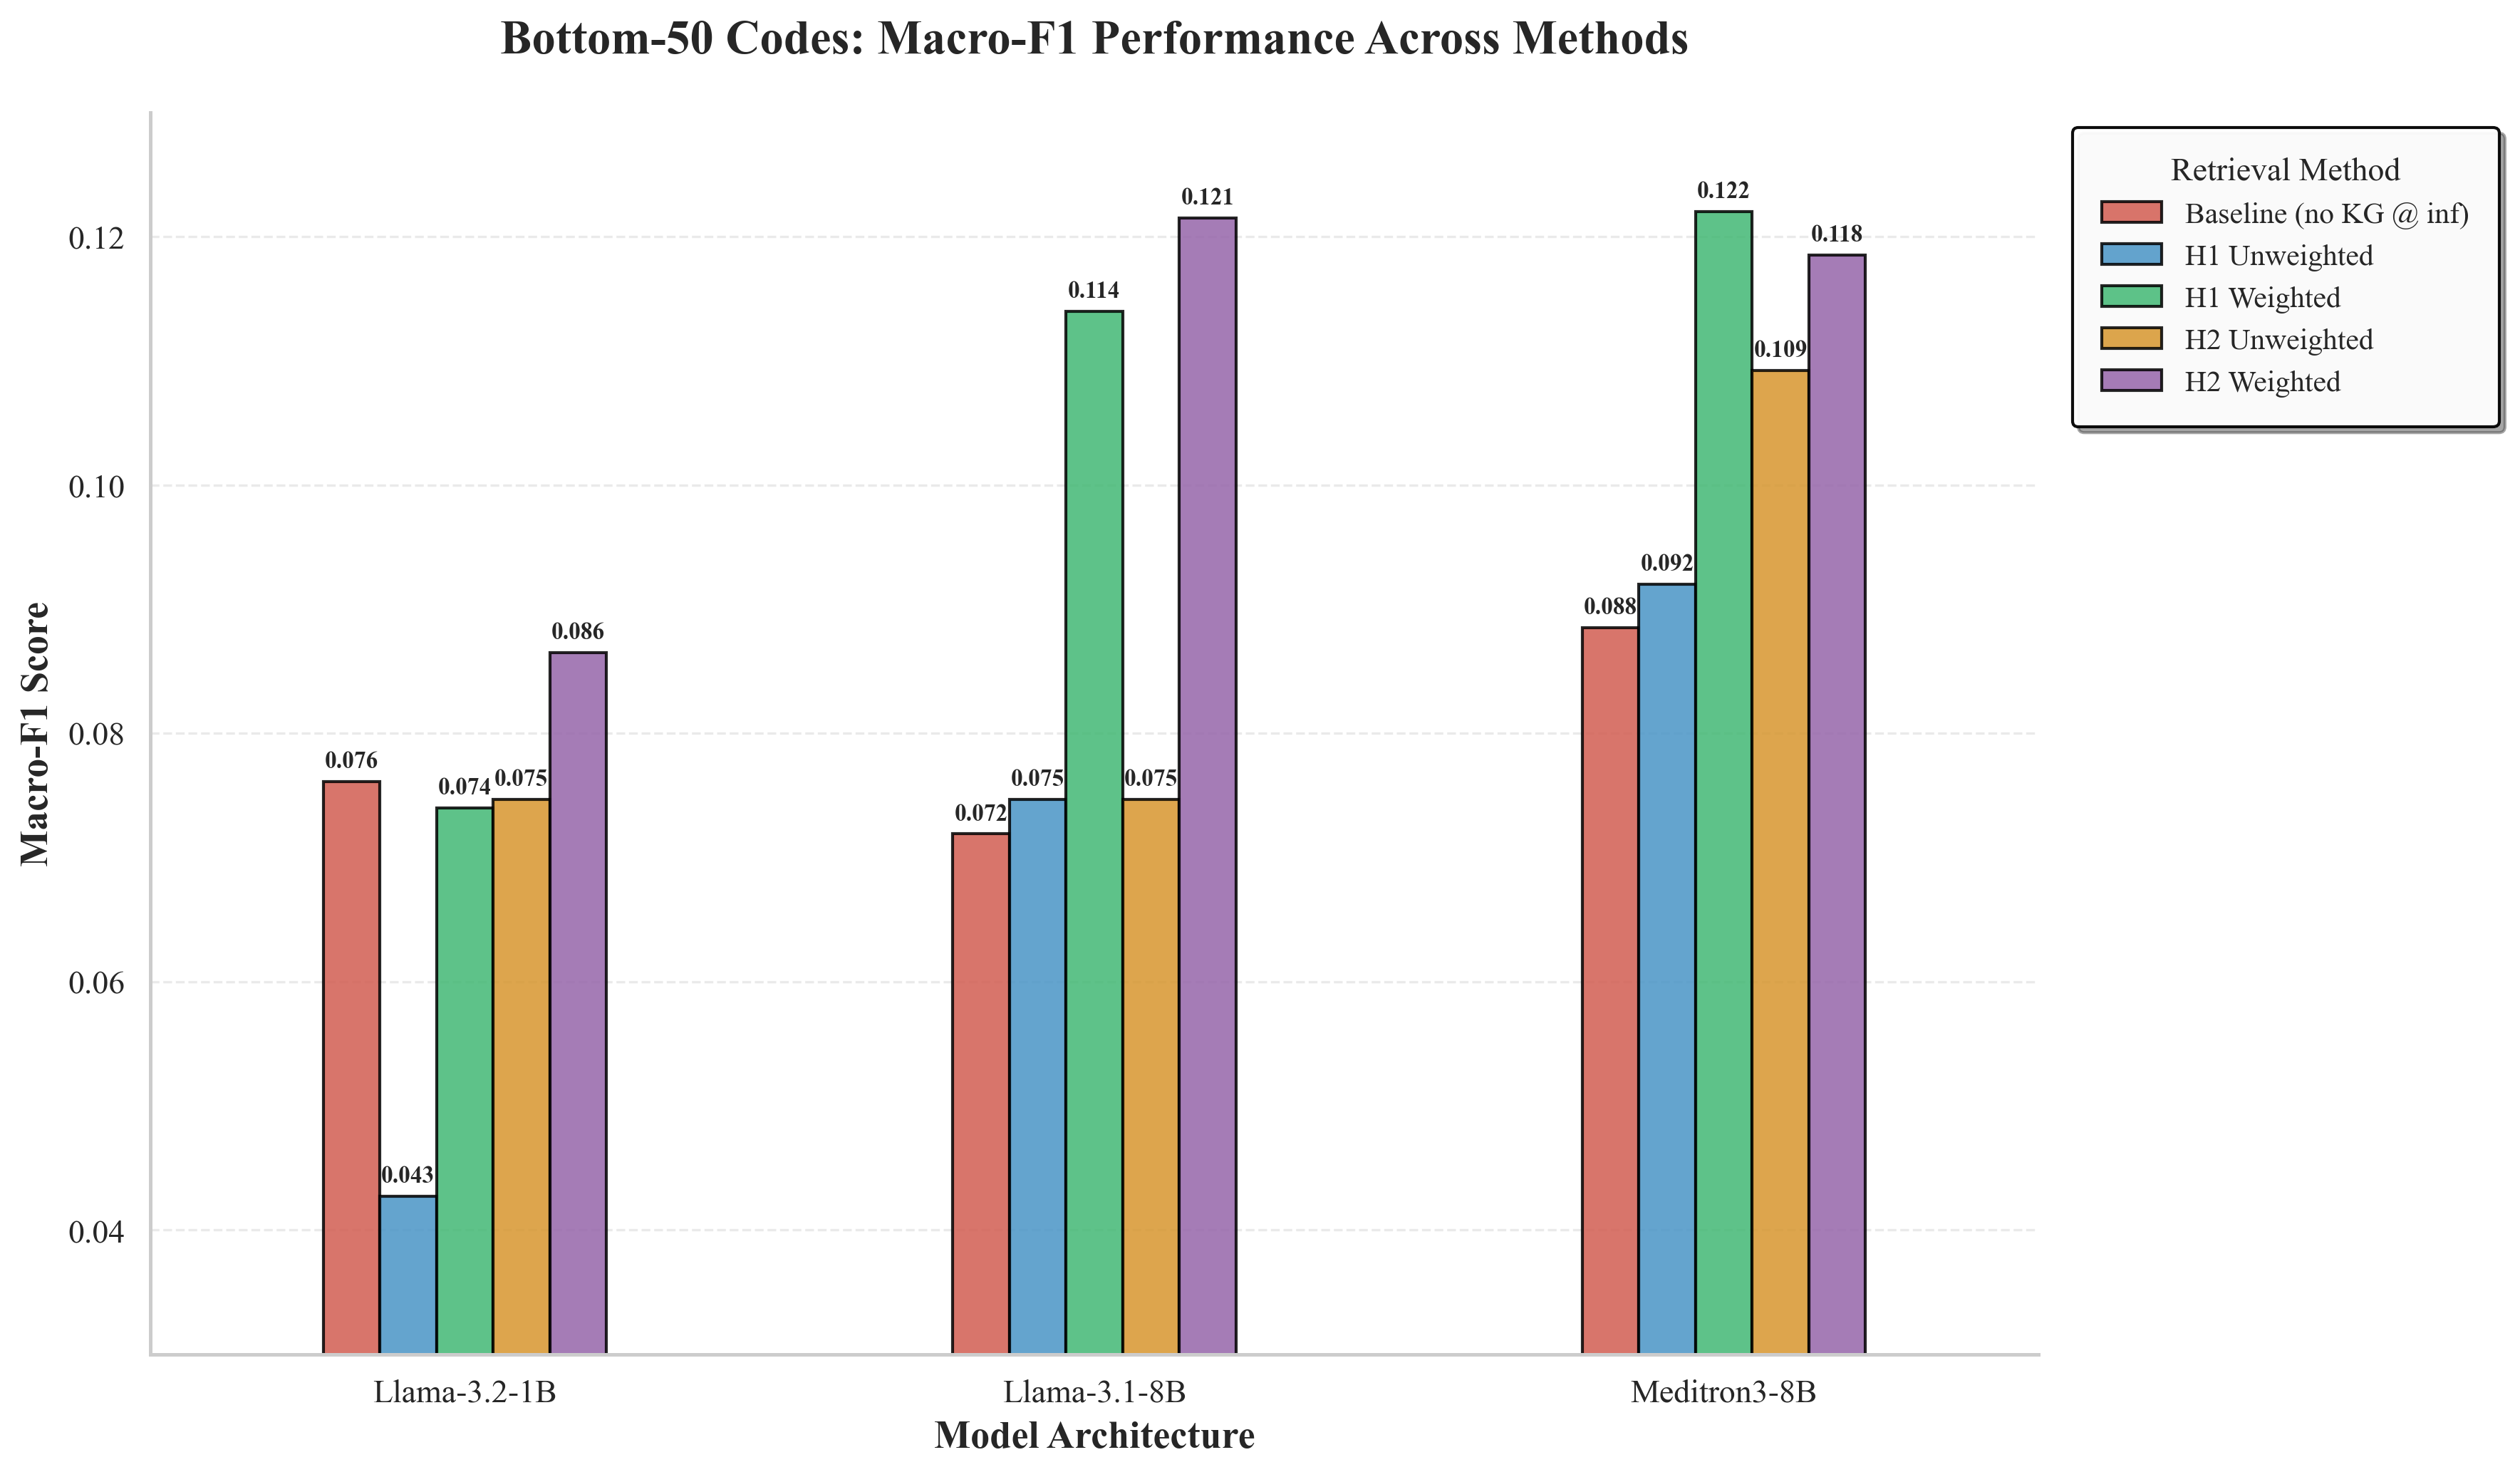
\includegraphics[width=\linewidth]{Images/h1vh2vbase/new/bottom50_macro_f1.png}
        \caption{Bottom50 macro-F1}
        \label{fig:task1-bottom50-macroF1}
    \end{subfigure}

    \caption{Task~1: KG/RAG head-tail plots: Head-50 vs Tail-50 micro-F1 (and/or macro-F1) for Baseline vs.\ KG variants.}
    \label{fig:task1-rag-headtail-plots}
\end{figure}

\paragraph{Interpretation: why Tail-50 improves under KG-augmented training.}
Tail codes suffer from sparse supervision and are easily crowded out under a strict 12-output budget. KG-augmented fine-tuning provides an additional inductive bias: retrieved relations can raise the \emph{salience} of clinically linked but underrepresented diagnoses, improving prioritisation. Empirically, Tail-50 micro-F1 improves for all backbones when moving from baseline to the best tail-performing KG variant:
\begin{itemize}
    \item \textbf{Llama-3.2-1B:} 0.1429 $\rightarrow$ 0.1841 (\,$\Delta{=}{+}0.0412$, +28.8\%).
    \item \textbf{Llama-3.1-8B:} 0.1250 $\rightarrow$ 0.1820 (\,$\Delta{=}{+}0.0570$, +45.6\%).
    \item \textbf{Meditron-8B:} 0.1518 $\rightarrow$ 0.1915 (\,$\Delta{=}{+}0.0397$, +26.2\%).
\end{itemize}
While absolute tail scores remain modest (rare-code recovery remains difficult), the directionality is consistent and aligns with the thesis motivation: structured relations can partially compensate for limited tail supervision.

% ============================================================
% \subsection{Interaction with Multimorbidity and the 12-Diagnosis Output Budget}
% \label{subsec:results-task1-budget}

% As shown in Fig.~\ref{fig:k_ablation}, increasing \(k\) improves Micro-F1 up to \(k=16\), after which both Micro-F1 and Macro-F1 saturate, indicating diminishing returns from allowing additional outputs. While \(k=16\) attains a marginally higher Micro-F1 than \(k=12\), it does so with lower precision and a higher average number of predicted terms per visit (\(\approx 10.69\) vs.\ \(9.47\)), increasing false positives and the downstream clinical review burden. In contrast, \(k=12\) provides a more balanced operating point: it yields a substantial recall gain over smaller \(k\) while maintaining comparatively higher precision, and it avoids the over-prediction regime where further increases in \(k\) primarily add low-confidence labels rather than meaningful performance improvements. Notably, the mean number of generated terms per visit plateaus at \(\approx 10.9\) for \(k \ge 20\) (Fig.~\ref{fig:k_saturation}), suggesting an intrinsic output saturation of the model and reinforcing \(k=12\) as a practical and conservative choice.

% Imposing a fixed output budget makes evaluation more realistic (clinical decision-support systems cannot output arbitrarily many diagnoses) but implies that recall improvements must come from \emph{prioritisation} of the most relevant codes. This is where KG-augmented fine-tuning is especially relevant: relational structure can provide additional cues to rank and select diagnoses effectively under a strict prediction budget. Under this constraint, the maximum achievable recall for admission \(i\) becomes
% \[
% R^{\max(i)} = \min\left(1, \frac{12}{L^{(i)}}\right),
% \]
% where \(L^{(i)}\) denotes the number of gold diagnoses for admission \(i\).

\subsection{Interaction with Multimorbidity and the 12-Diagnosis Output Budget}
\label{subsec:results-task1-budget}

Fig.~\ref{fig:k_ablation} reports a $k$-ablation where the system is constrained to output at most $k$ unique diagnoses per admission (after post-processing and de-duplication). We summarise performance using micro-averaged precision/recall at the operating budget ($P_{\text{micro}}@k$, $R_{\text{micro}}@k$) and the corresponding $F1_{\text{micro}}@k$, together with macro-F1 ($F1_{\text{macro}}@k$).

As $k$ increases, recall rises monotonically (Fig.~\ref{fig:k_pr_tradeoff}), but precision decreases, producing the expected precision--recall trade-off. Concretely, moving from $k=8$ to $k=12$ improves $F1_{\text{micro}}@k$ from $0.415$ to $0.461$ while increasing $R_{\text{micro}}@k$ from $0.323$ to $0.401$ (Fig.~\ref{fig:k_f1_trends}); precision drops from $P_{\text{micro}}@8=0.580$ to $P_{\text{micro}}@12=0.543$ (Fig.~\ref{fig:k_pr_tradeoff}). Increasing the budget further to $k=16$ yields only a marginal gain in $F1_{\text{micro}}@k$ (from $0.461$ to $0.470$), driven primarily by higher recall ($R_{\text{micro}}@16=0.429$) but at the cost of lower precision ($P_{\text{micro}}@16=0.520$). Beyond $k\ge 16$, both $F1_{\text{micro}}@k$ and $F1_{\text{macro}}@k$ plateau (approximately $F1_{\text{micro}}@k\approx 0.470$ and $F1_{\text{macro}}@k\approx 0.223$), indicating diminishing returns from allowing additional outputs.

From a deployment perspective, $k=12$ is selected as a conservative and clinically practical operating point. While $k=16$ slightly increases $F1_{\text{micro}}$, it also increases the average number of predicted terms per visit (Fig.~\ref{fig:k_saturation}; $\approx 9.5$ at $k=12$ vs.\ $\approx 10.7$ at $k=16$), which translates to more false positives and a higher downstream review burden. Moreover, the generation process itself exhibits an intrinsic saturation: the mean number of generated terms per visit plateaus at $\approx 10.9$ for $k\ge 20$ (Fig.~\ref{fig:k_saturation}), so larger budgets leave increasing unused capacity and do not yield additional practical benefit.

Imposing a fixed output budget makes evaluation more realistic (clinical decision-support systems cannot output arbitrarily many diagnoses) but implies that recall improvements must come from \emph{prioritisation} of the most relevant labels under limited slots. Under this constraint, the maximum achievable recall for admission $i$ becomes
\[
R^{\max(i)}=\min\left(1,\frac{12}{L^{(i)}}\right),
\]
where $L^{(i)}$ denotes the number of gold diagnoses for admission $i$. This budgeted regime is precisely where KG-augmented training is most relevant: relational evidence can help rank and select plausible diagnoses more effectively under strict $k$.
\begin{figure*}[t]
    \centering
    \begin{subfigure}[b]{0.45\textwidth}
        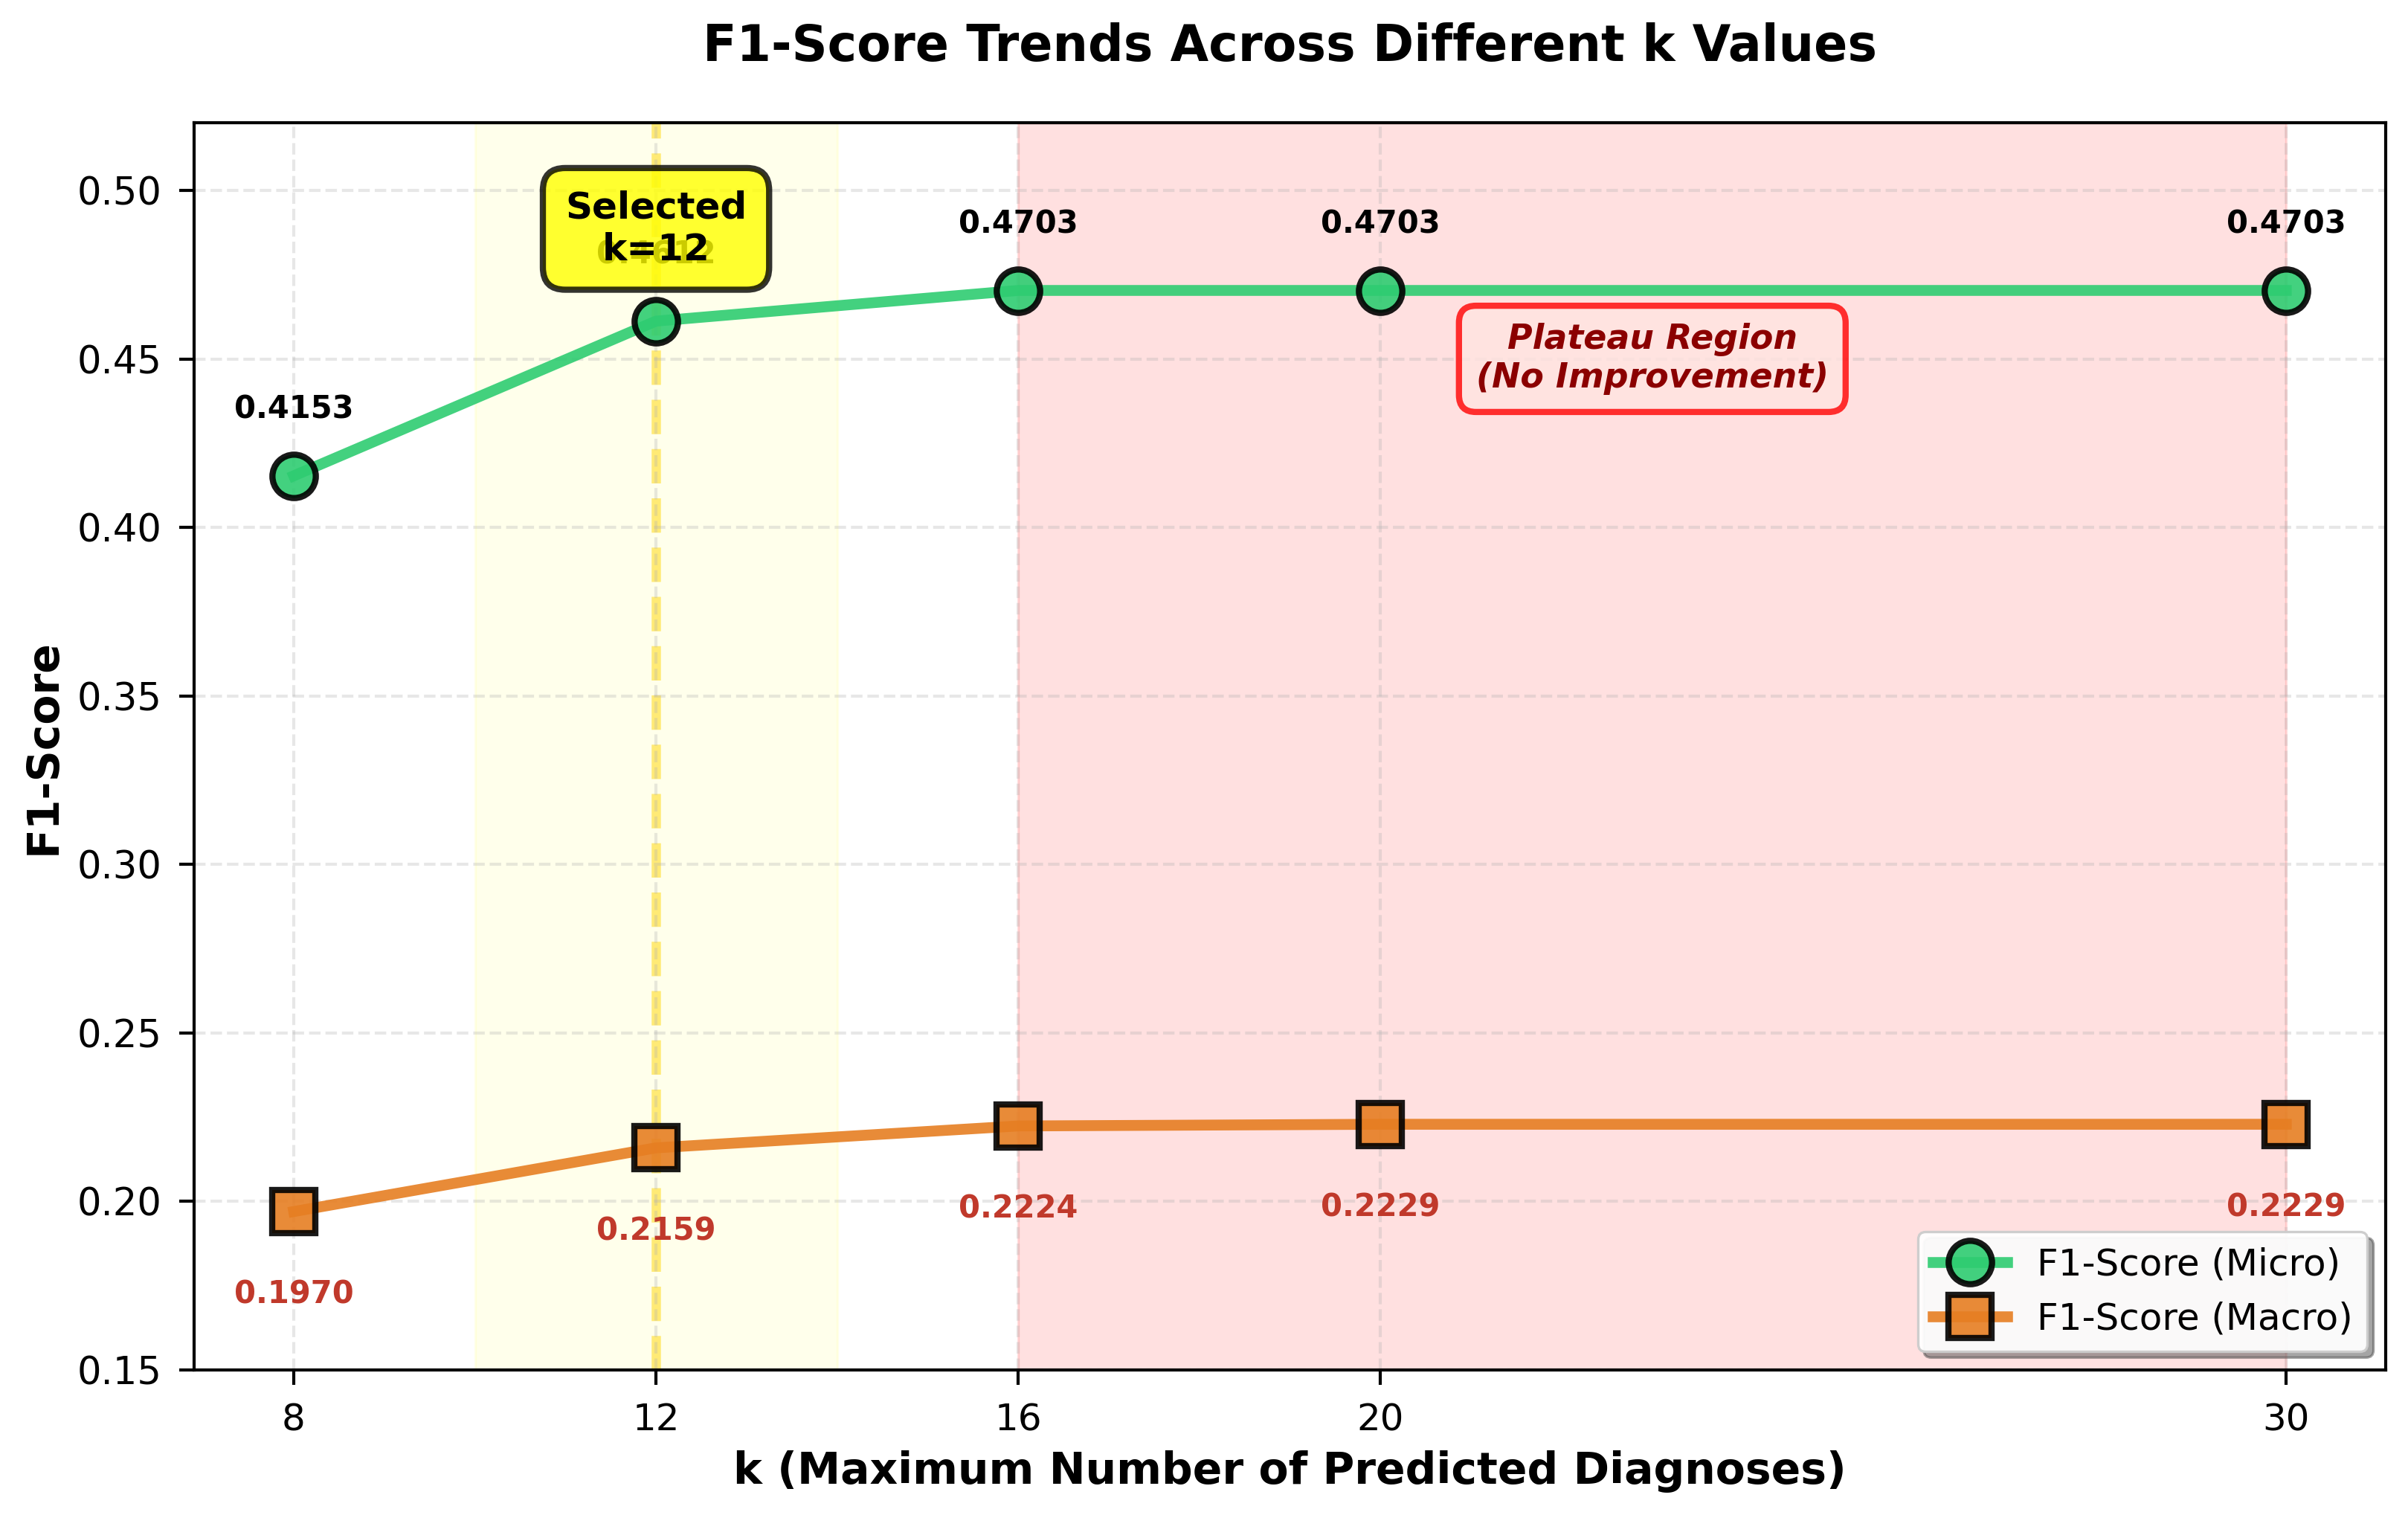
\includegraphics[width=\textwidth]{Images/k_ablation_f1_trends.png}
        \caption{F1 trends (Micro/Macro) vs.\ \(k\)}
        \label{fig:k_f1_trends}
    \end{subfigure}
    \hfill
    \begin{subfigure}[b]{0.45\textwidth}
        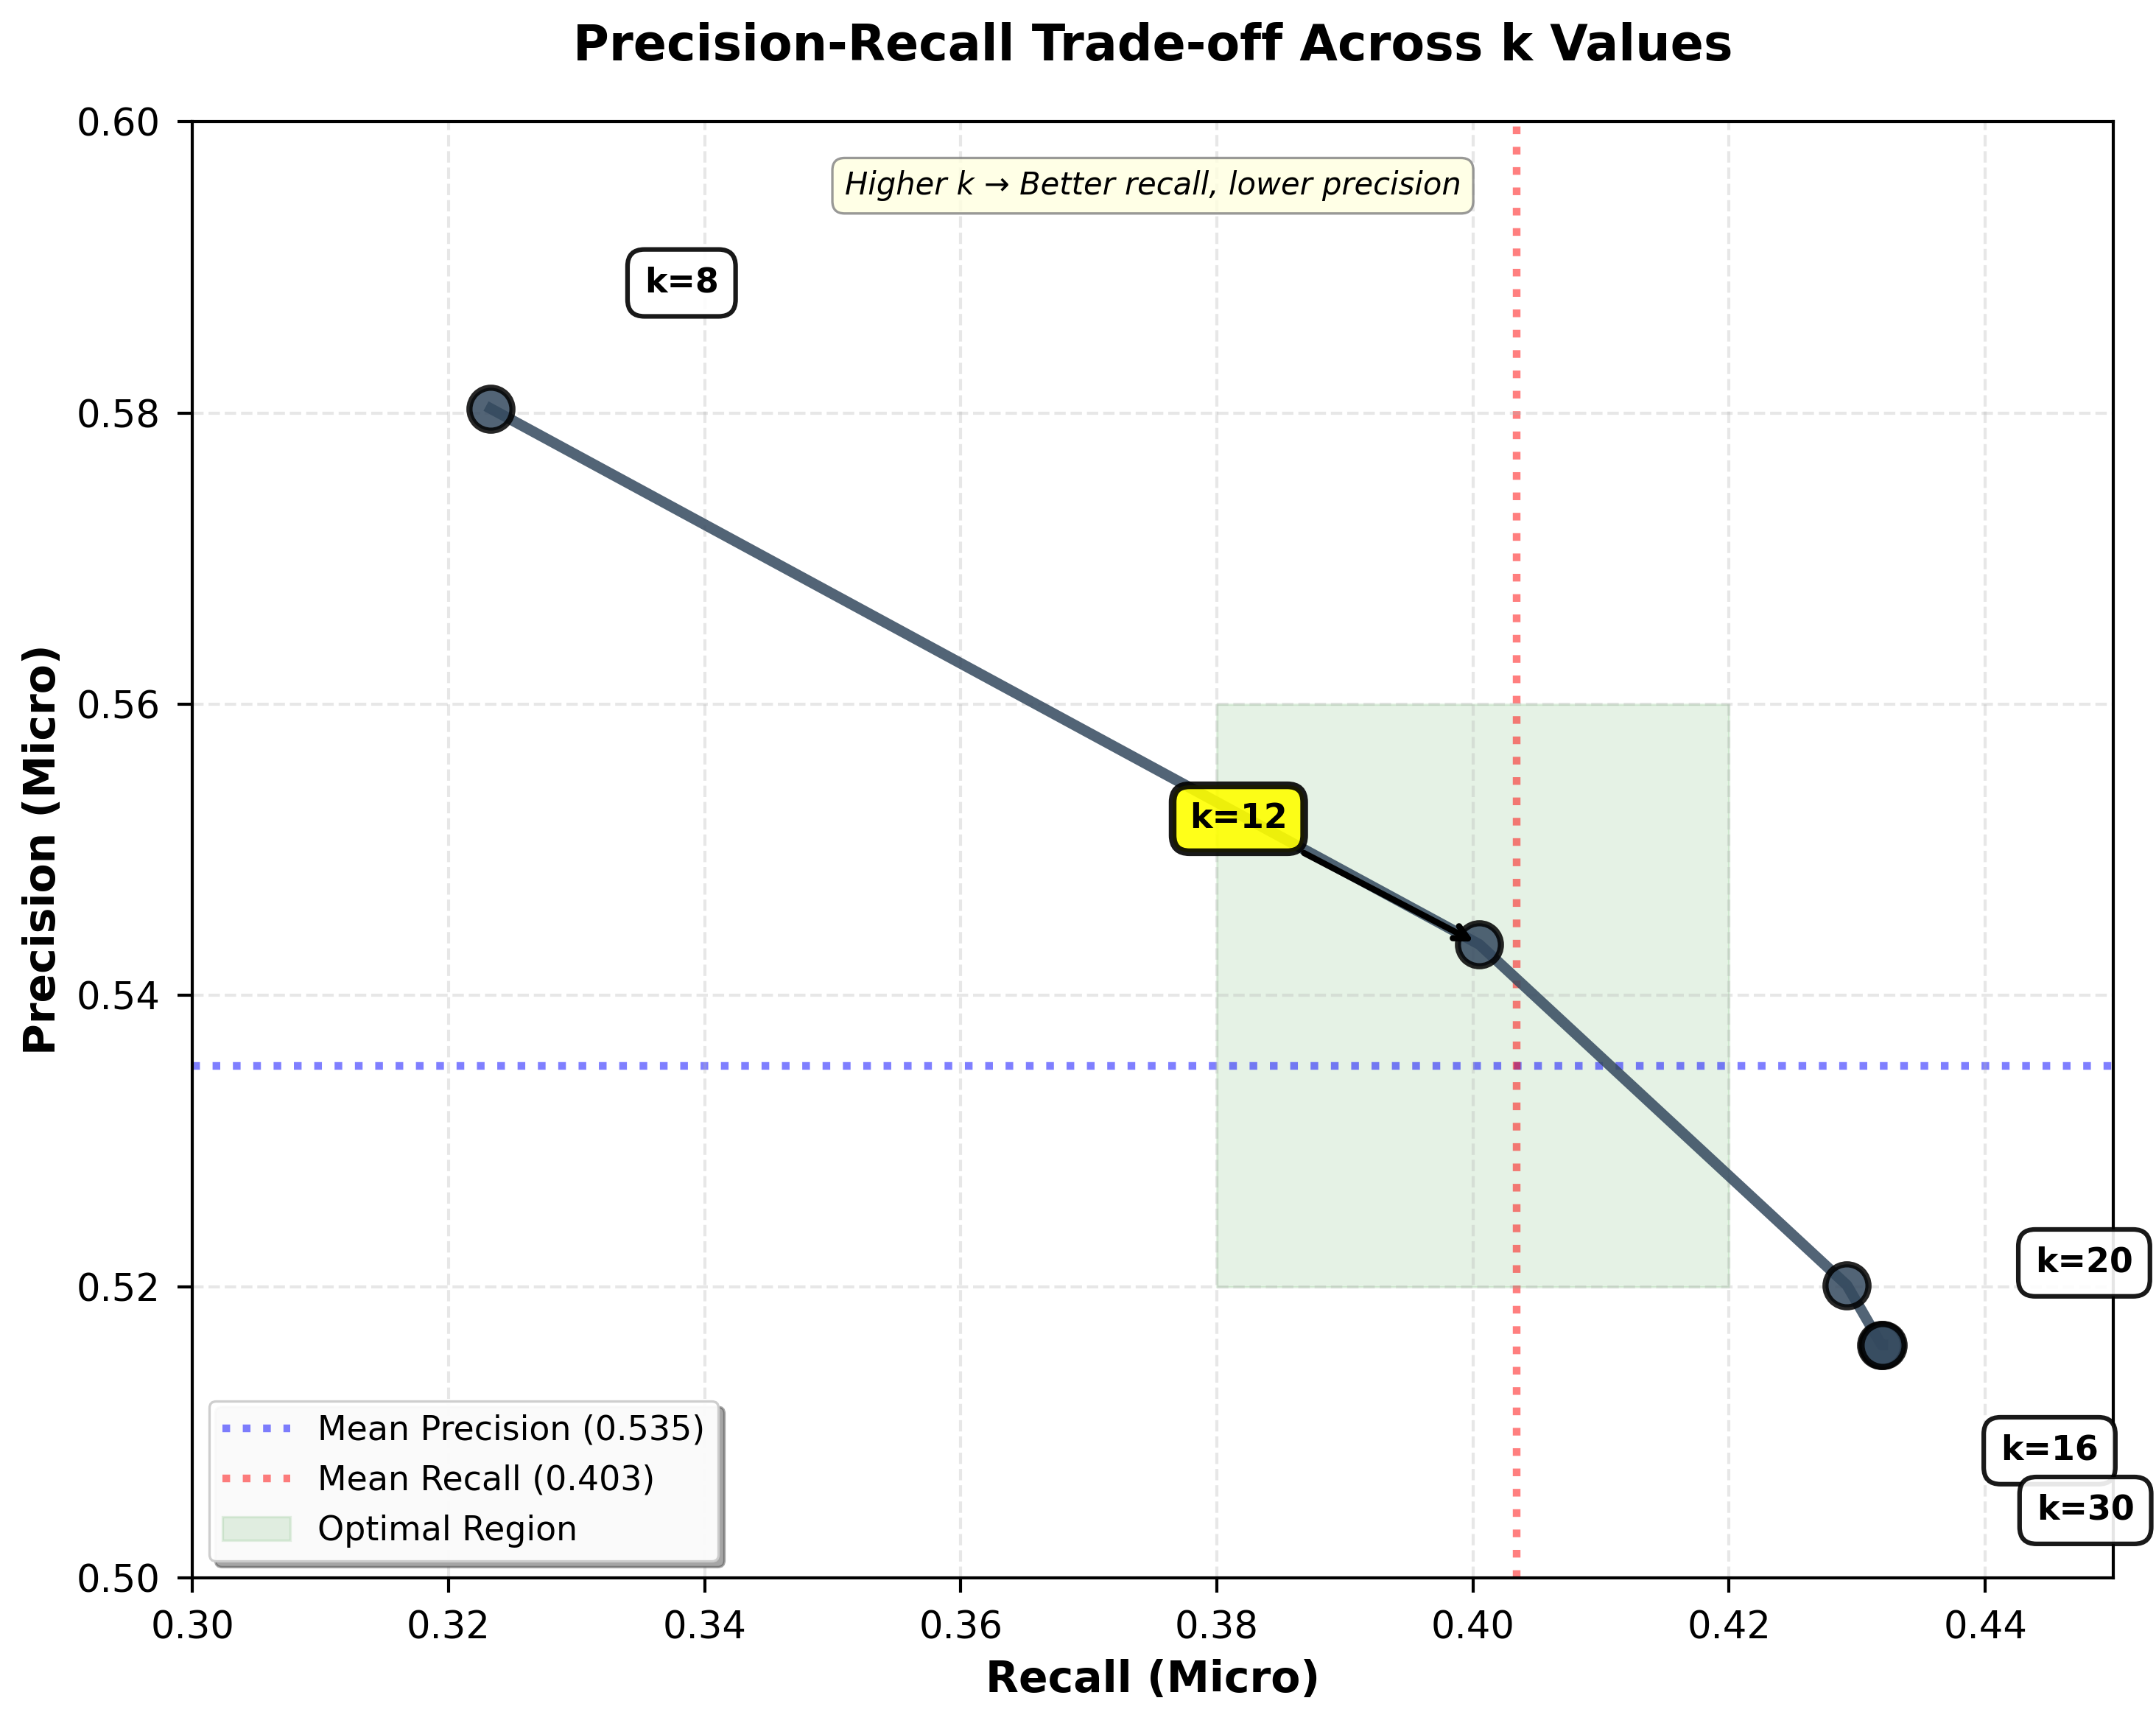
\includegraphics[width=\textwidth]{Images/k_ablation_precision_recall.png}
        \caption{Precision--recall trade-off}
        \label{fig:k_pr_tradeoff}
    \end{subfigure}
    \hfill
    \begin{subfigure}[b]{0.45\textwidth}
        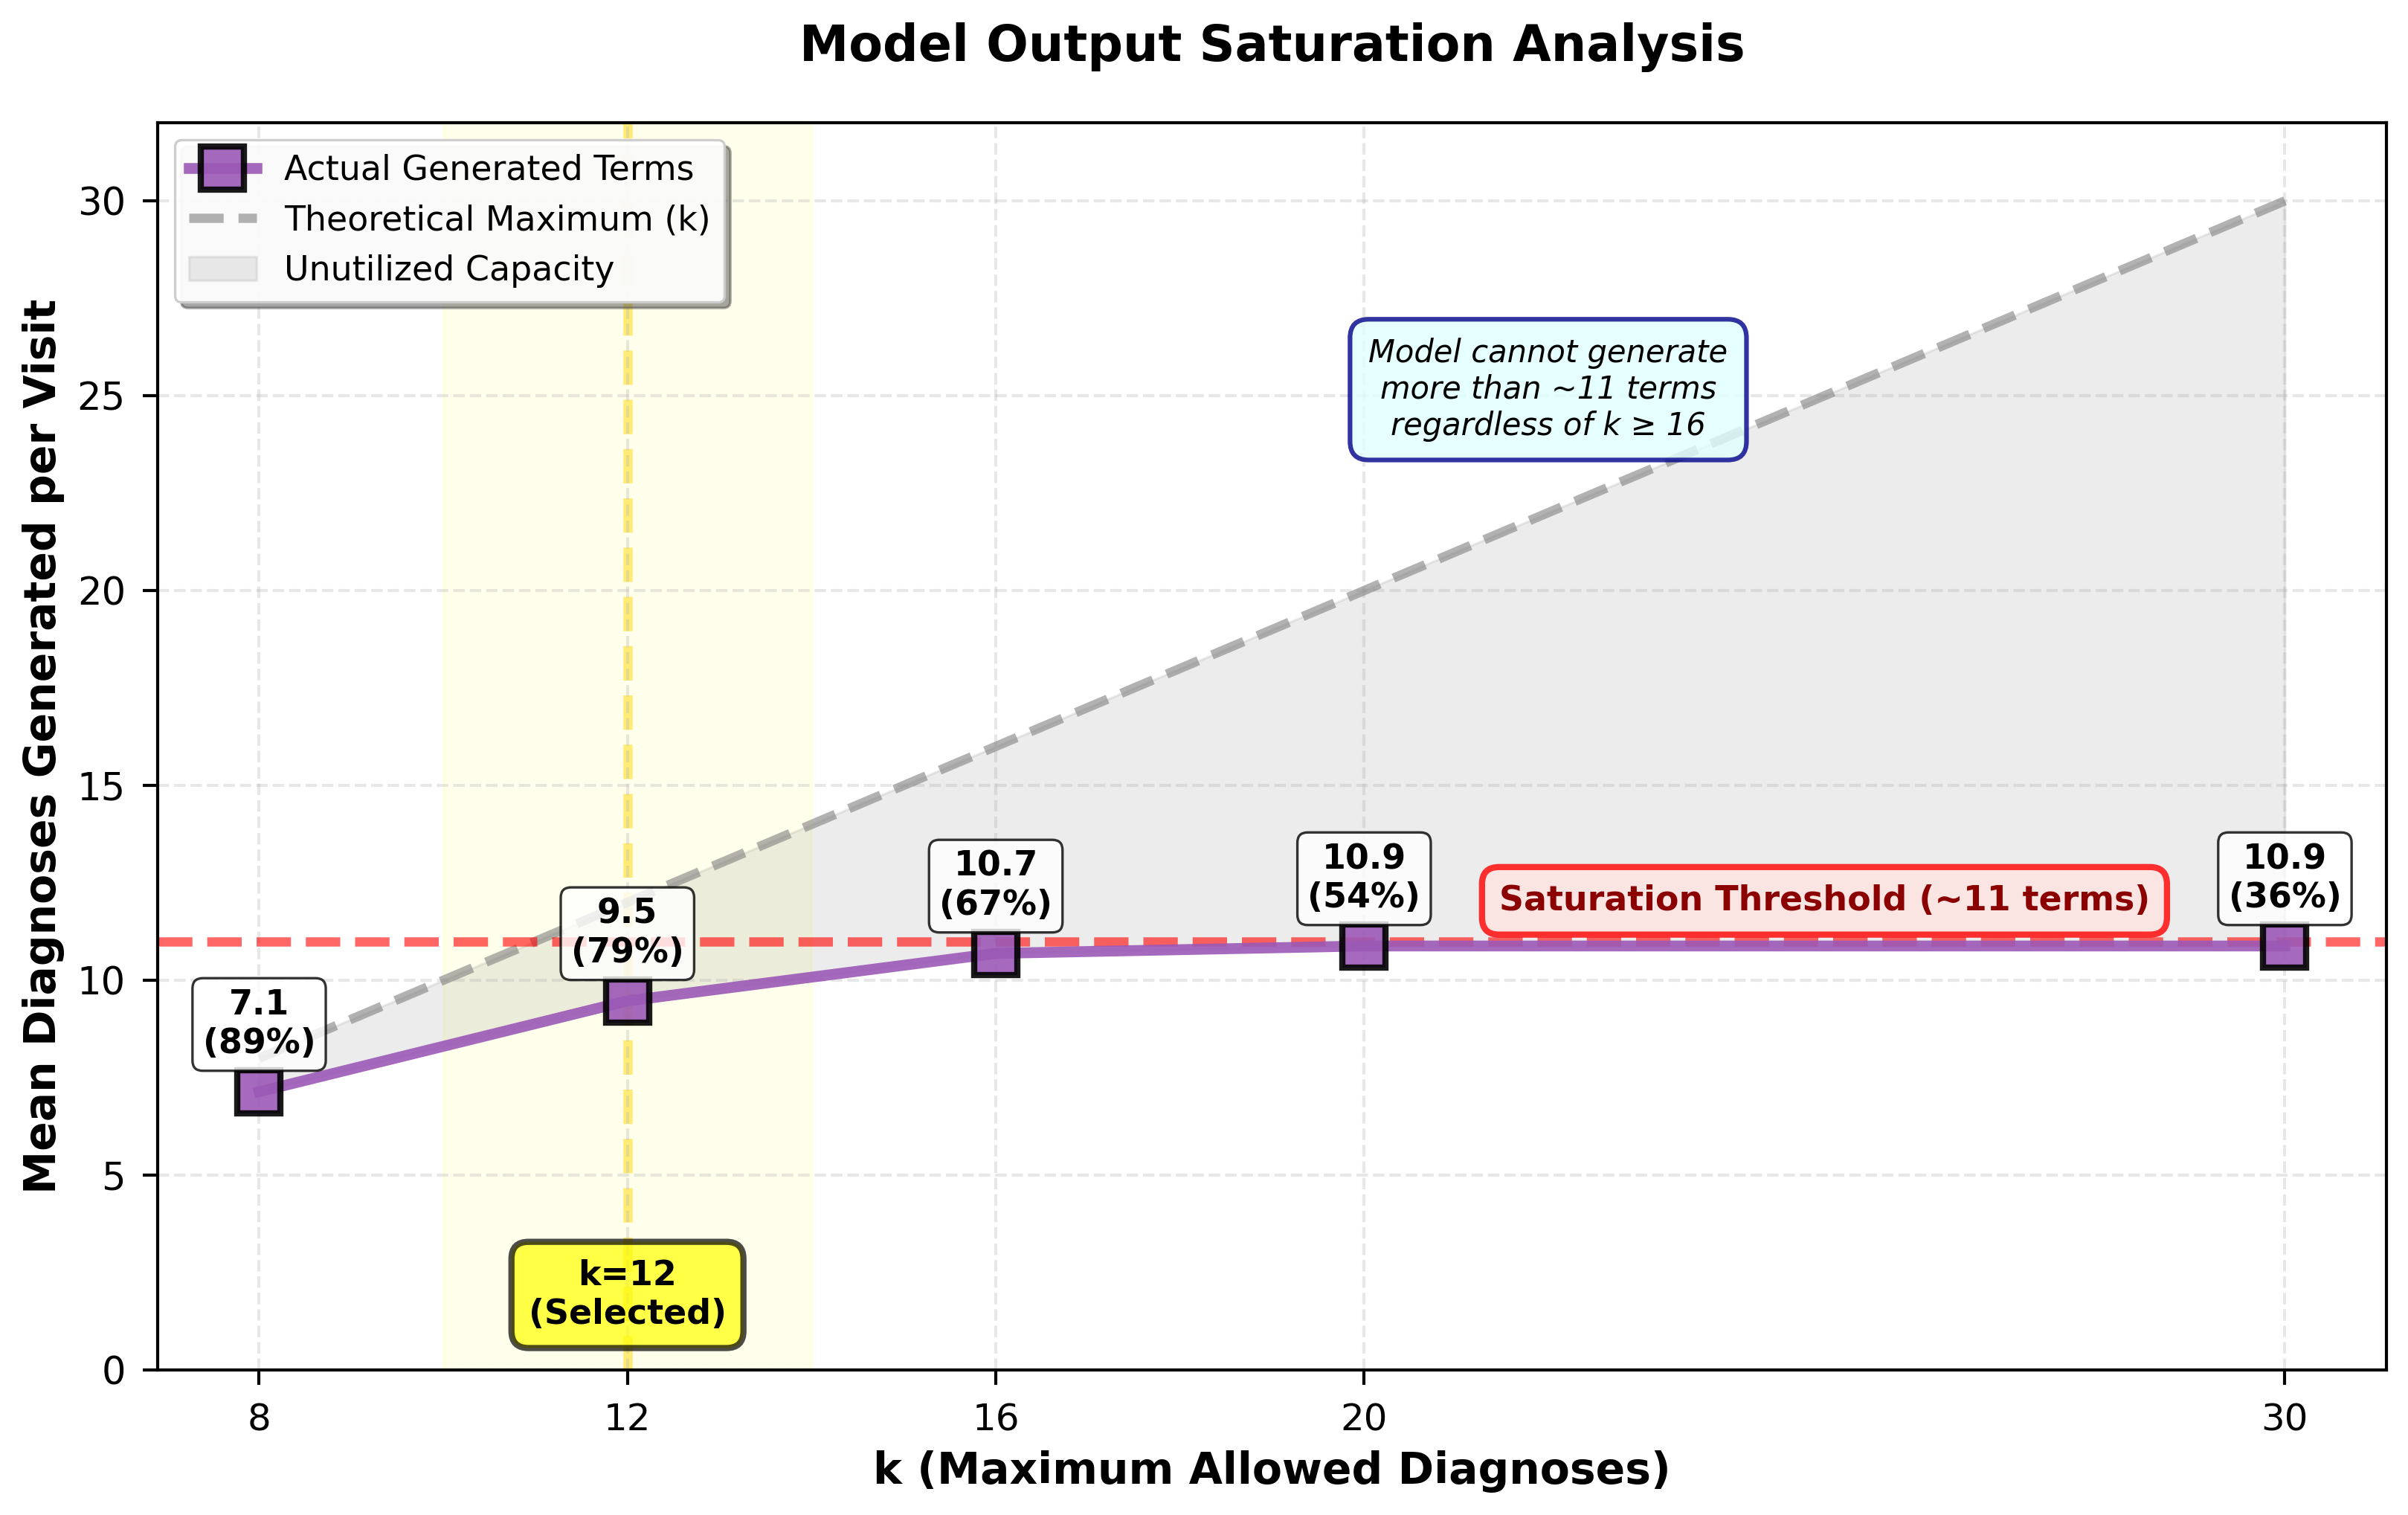
\includegraphics[width=\textwidth]{Images/k_ablation_saturation.png}
        \caption{Mean terms/visit and saturation}
        \label{fig:k_saturation}
    \end{subfigure}
    \caption{\textbf{K-ablation study.} Increasing \(k\) improves performance up to \(k=16\), after which metrics plateau. The precision--recall curve highlights the trade-off as \(k\) increases, while the mean predicted terms/visit saturate, indicating limited benefit from larger output budgets.}
    \label{fig:k_ablation}
\end{figure*}

% ============================================================
\subsection{Summary}
\label{subsec:results-task1-summary}

Task~1 results form a coherent progression:
\begin{itemize}
    \item \textbf{Strong baseline:} fine-tuned TextGen provides a clean and competitive reference point compared to Base and CodeGen.
    \item \textbf{Inference-only KG ablation:} injecting KG paths at inference without KG-aware training does not improve performance and typically degrades it, consistent with the hypothesis that na\"ive KG injection can introduce noise and distract generation.
    \item \textbf{KG-augmented fine-tuning helps:} RAG-style variants produce consistent gains over the best baseline across overall, parent-level, and frequency-sliced evaluation, with the most meaningful improvements observed on Tail-50 codes.
\end{itemize}

To make improvements explicit, Table~\ref{tab:task1-delta-summary-final} summarises absolute ($\Delta$) and relative (\%) gains from Baseline TextGen (no KG at inference) to the best KG-augmented variant per backbone (chosen by overall micro-F1). For the tail, we additionally report the best tail-performing KG variant (which may differ from the overall-best choice).

\begin{table}[t]
\centering
\caption{Improvements from Baseline TextGen (no KG at inference) to best KG-augmented variant per backbone (selected by overall micro-F1). Tail improvements are reported for the best tail-performing KG variant. Relative gains shown as percent.}
\label{tab:task1-delta-summary-final}
\resizebox{\textwidth}{!}{
\begin{tabular}{lcccccc}
\toprule
\textbf{Backbone} &
\textbf{Overall micro-F1} & $\Delta$ (\%) &
\textbf{Overall macro-F1} & $\Delta$ (\%) &
\textbf{Tail-50 micro-F1} & $\Delta$ (\%) \\
\midrule
Llama-3.2-1B &
0.4313 $\rightarrow$ 0.4749 & +0.0436 (+10.1\%) &
0.2065 $\rightarrow$ 0.2368 & +0.0303 (+14.7\%) &
0.1429 $\rightarrow$ 0.1841 & +0.0412 (+28.8\%) \\
\midrule
Llama-3.1-8B &
0.4585 $\rightarrow$ 0.5029 & +0.0444 (+9.7\%) &
0.2457 $\rightarrow$ 0.2762 & +0.0305 (+12.4\%) &
0.1250 $\rightarrow$ 0.1820 & +0.0570 (+45.6\%) \\
\midrule
Meditron-8B &
0.4585 $\rightarrow$ 0.5036 & +0.0451 (+9.8\%) &
0.2457 $\rightarrow$ 0.2793 & +0.0336 (+13.7\%) &
0.1518 $\rightarrow$ 0.1915 & +0.0397 (+26.2\%) \\
\bottomrule
\end{tabular}}
\end{table}

\noindent\textbf{Conclusive statement.}
With a strong fine-tuned TextGen baseline, inference-only KG injection fails to improve performance, indicating that \emph{prompt-time grounding alone is insufficient}. In contrast, KG-augmented fine-tuning yields consistent gains in both overall metrics and Tail-50 recovery. This supports the conclusion that \emph{structured knowledge improves diagnosis prediction only when the model is explicitly trained to interpret and leverage KG evidence}, and that the main benefit manifests as improved prioritisation of underrepresented diagnoses under a strict prediction budget.


\section{Task~2: Next-Visit Diagnosis Prediction}
\label{sec:results-task2}

This section reports results for Task~2 (history-aware, next-visit diagnosis prediction) under the evaluation protocol in Section~\ref{sec:evaluation}. Building on Task~1, we directly adopt \textbf{TextGen} as the default pipeline (fine-tuned diagnosis-term generation followed by SapBERT+FAISS semantic mapping), because it consistently outperformed Base and CodeGen baselines in Task~1 (Section~\ref{sec:results-task1}). We evaluate the same three backbones (\texttt{Llama-3.2-1B-Instruct}, \texttt{Llama-3.1-8B-Instruct}, \texttt{Meditron-8B}).

\paragraph{Experimental progression (Task~2).}
We follow a streamlined progression consistent with the Task~1 story but adapted to the history-aware setup:
\begin{enumerate}
    \item \textbf{Strong baseline:} fine-tune TextGen for next-visit prediction (history-aware prompt; no KG facts).
    \item \textbf{KG/RAG at inference:} keep the trained model fixed and augment \emph{only the inference prompt} with retrieved KG paths (H1/H2; weighted/unweighted).
\end{enumerate}
Thus, Task~2 evaluates whether \emph{prompt-time grounding alone} provides measurable benefit when the model is already conditioned on longitudinal patient history.

As in Task~1 (Section~\ref{subsec:complexity-cohort}), all models are instructed to output a fixed budget of \textbf{at most 12 diagnoses} per admission, which constrains recall under high multimorbidity and can make small metric differences difficult to interpret without uncertainty estimates.

% ============================================================
\subsection{TextGen Baseline for History-Aware Next-Visit Prediction}
\label{subsec:results-task2-baseline}

We first establish a clean reference point by fine-tuning TextGen for next-visit prediction. Table~\ref{tab:task2-overall} (Baseline rows) reports overall code-level metrics on the held-out test set. Compared to Task~1, absolute micro-F1 is lower across backbones, reflecting the intrinsic difficulty of predicting a \emph{future} diagnostic set rather than reconstructing diagnoses supported directly by the current admission.

\begin{figure}[t]
    \centering
    
\includegraphics[width=0.92\textwidth]{Images/Empty.png}
    \caption{(Placeholder) Task~2 baseline metrics: overall micro/macro precision, recall, and F1 for the history-aware TextGen baseline across backbones.}
    \label{fig:task2-baseline-overall-plots}
\end{figure}

% ============================================================
\subsection{Ablation: KG/RAG Augmentation at Inference Only}
\label{subsec:results-task2-kg-inference}

We next test whether retrieved KG paths help \emph{without changing training}. Concretely, we keep the fine-tuned Task~2 TextGen checkpoint fixed and augment only the inference prompt with KG evidence:
(i) \textbf{H1} vs.\ \textbf{H2} (different hop-depth/retrieval scopes), and
(ii) \textbf{Unweighted} vs.\ \textbf{Weighted} (raw concatenation vs.\ relevance-weighted selection/scoring of facts).

% -----------------------------
\subsubsection{Overall code-level metrics}
\label{subsubsec:results-task2-overall}

Table~\ref{tab:task2-overall} shows that KG augmentation yields \textbf{very small changes} in overall micro-F1 and macro-F1. The best variants per backbone improve micro-F1 by only $\approx$0.001--0.006 absolute, and macro-F1 changes are mixed. Given that these deltas are within the range typically attributable to sampling variance for rare-label multilabel problems, these results suggest that \textbf{inference-only KG prompting provides limited additional signal} once the model is already conditioned on longitudinal history.

\begin{table}[t]
\centering
\caption{Task~2 overall code-level metrics (test set). \textbf{Baseline} is the history-aware TextGen system. KG variants augment \emph{only inference prompts} with retrieved KG paths (H1/H2; weighted/unweighted).}
\label{tab:task2-overall}
\resizebox{\textwidth}{!}{
\begin{tabular}{llcccccc}
\toprule
\textbf{Model} & \textbf{Mode} &
\textbf{Micro-F1} & \textbf{Micro-P} & \textbf{Micro-R} &
\textbf{Macro-F1} & \textbf{Macro-P} & \textbf{Macro-R} \\
\midrule
Meditron3-8B & Baseline & 0.4172 & 0.5120 & 0.3521 & 0.1714 & 0.2347 & 0.1598 \\
Meditron3-8B & H1 Unweighted & 0.4176 & 0.5122 & 0.3525 & 0.1701 & 0.2344 & 0.1593 \\
Meditron3-8B & H1 Weighted & 0.4178 & 0.5111 & 0.3533 & 0.1673 & 0.2287 & 0.1581 \\
Meditron3-8B & H2 Unweighted & 0.4152 & 0.5063 & 0.3519 & 0.1736 & 0.2376 & 0.1632 \\
Meditron3-8B & H2 Weighted & \textbf{0.4181} & 0.5103 & 0.3541 & \textbf{0.1745} & 0.2364 & 0.1640 \\
\midrule
Llama-3.1-8B & Baseline & 0.4154 & 0.5081 & 0.3514 & 0.1734 & 0.2409 & 0.1629 \\
Llama-3.1-8B & H1 Unweighted & 0.4178 & 0.5057 & 0.3559 & 0.1727 & 0.2331 & 0.1641 \\
Llama-3.1-8B & H1 Weighted & \textbf{0.4198} & 0.5119 & 0.3558 & 0.1727 & 0.2406 & 0.1602 \\
Llama-3.1-8B & H2 Unweighted & 0.4160 & 0.5047 & 0.3538 & 0.1683 & 0.2337 & 0.1573 \\
Llama-3.1-8B & H2 Weighted & 0.4188 & 0.5142 & 0.3533 & \textbf{0.1735} & 0.2362 & 0.1623 \\
\midrule
Llama-3.2-1B & Baseline & 0.3826 & 0.4596 & 0.3278 & 0.1411 & 0.1932 & 0.1350 \\
Llama-3.2-1B & H1 Unweighted & 0.3865 & 0.4667 & 0.3299 & 0.1420 & 0.1926 & 0.1357 \\
Llama-3.2-1B & H1 Weighted & 0.3854 & 0.4642 & 0.3295 & \textbf{0.1431} & 0.1913 & 0.1378 \\
Llama-3.2-1B & H2 Unweighted & \textbf{0.3890} & 0.4684 & 0.3326 & 0.1376 & 0.1893 & 0.1297 \\
Llama-3.2-1B & H2 Weighted & 0.3853 & 0.4649 & 0.3291 & 0.1429 & 0.1953 & 0.1357 \\
\bottomrule
\end{tabular}}
\end{table}

\begin{figure}[t]
    \centering
    
\includegraphics[width=0.92\textwidth]{Images/Empty.png}
    \caption{(Placeholder) Task~2 overall metrics: grouped bars (micro/macro P/R/F1) comparing Baseline vs.\ H1/H2 (weighted/unweighted) per backbone.}
    \label{fig:task2-overall-plots}
\end{figure}

\paragraph{Interpretation.}
Two consistent patterns emerge:
\begin{itemize}
    \item \textbf{Changes are marginal at the full-code level.} The history-aware baseline already provides strong context; KG evidence added at inference does not substantially shift overall precision/recall.
    \item \textbf{Weighting is not consistently beneficial in Task~2.} Unlike Task~1 (where weighted KG often helped), Task~2 shows mixed effects, suggesting that relevance scoring optimized for current-visit grounding may not translate directly to forecasting the next visit.
\end{itemize}

% -----------------------------
\subsubsection{Head--tail analysis}
\label{subsubsec:results-task2-headtail}

To characterise label imbalance explicitly, we evaluate the same global \textbf{Head-50} and \textbf{Tail-50} ICD-9 code subsets used in Task~1 (defined by frequency across all splits). Tables~\ref{tab:task2-top50} and \ref{tab:task2-bottom50} report these results.

\paragraph{Head-50 (frequent codes).}
Table~\ref{tab:task2-top50} shows that baseline performance on frequent labels is strong and KG variants yield only small changes. This is consistent with the overall results: frequent-code performance is relatively stable under prompt perturbations.

\begin{table}[t]
\centering
\caption{Task~2 performance restricted to the Top-50 most frequent ICD-9 codes (Head-50).}
\label{tab:task2-top50}
\resizebox{\textwidth}{!}{
\begin{tabular}{llcccccc}
\toprule
\textbf{Model} & \textbf{Mode} &
\textbf{Micro-F1} & \textbf{Micro-P} & \textbf{Micro-R} &
\textbf{Macro-F1} & \textbf{Macro-P} & \textbf{Macro-R} \\
\midrule
Meditron3-8B & Baseline & 0.5841 & 0.6177 & 0.5540 & 0.4804 & 0.5530 & 0.4665 \\
Meditron3-8B & H1 Unweighted & 0.5827 & 0.6141 & 0.5543 & 0.4786 & 0.5508 & 0.4642 \\
Meditron3-8B & H1 Weighted & 0.5816 & 0.6086 & 0.5569 & 0.4785 & 0.5573 & 0.4679 \\
Meditron3-8B & H2 Unweighted & 0.5774 & 0.6061 & 0.5514 & 0.4733 & 0.5451 & 0.4612 \\
Meditron3-8B & H2 Weighted & 0.5823 & 0.6136 & 0.5541 & 0.4801 & 0.5558 & 0.4654 \\
\midrule
Llama-3.1-8B & Baseline & 0.5770 & 0.6072 & 0.5496 & 0.4753 & 0.5513 & 0.4597 \\
Llama-3.1-8B & H1 Unweighted & 0.5802 & 0.6077 & 0.5551 & 0.4775 & 0.5440 & 0.4654 \\
Llama-3.1-8B & H1 Weighted & \textbf{0.5843} & 0.6122 & 0.5587 & \textbf{0.4834} & 0.5585 & 0.4688 \\
Llama-3.1-8B & H2 Unweighted & 0.5802 & 0.6055 & 0.5570 & 0.4797 & 0.5470 & 0.4679 \\
Llama-3.1-8B & H2 Weighted & 0.5839 & 0.6175 & 0.5537 & 0.4779 & 0.5509 & 0.4619 \\
\midrule
Llama-3.2-1B & Baseline & 0.5540 & 0.5719 & 0.5372 & 0.4557 & 0.5061 & 0.4509 \\
Llama-3.2-1B & H1 Unweighted & 0.5576 & 0.5788 & 0.5379 & 0.4603 & 0.5134 & 0.4517 \\
Llama-3.2-1B & H1 Weighted & \textbf{0.5580} & 0.5810 & 0.5368 & 0.4590 & 0.5092 & 0.4488 \\
Llama-3.2-1B & H2 Unweighted & 0.5528 & 0.5576 & \textbf{0.5481} & \textbf{0.4676} & 0.5215 & \textbf{0.4604} \\
Llama-3.2-1B & H2 Weighted & 0.5576 & 0.5791 & 0.5377 & 0.4602 & \textbf{0.5196} & 0.4520 \\
\bottomrule
\end{tabular}}
\end{table}

\paragraph{Tail-50 (rare codes).}
Table~\ref{tab:task2-bottom50} shows \textbf{high instability} for rare diagnoses. Several variants produce exactly zero Tail-50 scores despite non-zero baseline (or vice versa). This indicates that tail evaluation for next-visit prediction is extremely sensitive to a handful of true positives under the strict 12-output constraint, and that inference-time KG prompting can easily perturb which rare codes enter the limited output set.

\begin{table}[t]
\centering
\caption{Task~2 performance restricted to the Bottom-50 rarest ICD-9 codes (Tail-50). Tail metrics are high-variance due to extremely low support.}
\label{tab:task2-bottom50}
\resizebox{\textwidth}{!}{
\begin{tabular}{llcccccc}
\toprule
\textbf{Model} & \textbf{Mode} &
\textbf{Micro-F1} & \textbf{Micro-P} & \textbf{Micro-R} &
\textbf{Macro-F1} & \textbf{Macro-P} & \textbf{Macro-R} \\
\midrule
Meditron3-8B & Baseline & 0.0909 & 0.5000 & 0.0500 & 0.0444 & 0.0667 & 0.0333 \\
Meditron3-8B & H1 Unweighted & 0.0000 & 0.0000 & 0.0000 & 0.0000 & 0.0000 & 0.0000 \\
Meditron3-8B & H1 Weighted & 0.0000 & 0.0000 & 0.0000 & 0.0000 & 0.0000 & 0.0000 \\
Meditron3-8B & H2 Unweighted & \textbf{0.0952} & \textbf{1.0000} & 0.0500 & 0.0444 & 0.0667 & 0.0333 \\
Meditron3-8B & H2 Weighted & \textbf{0.0952} & \textbf{1.0000} & 0.0500 & 0.0444 & 0.0667 & 0.0333 \\
\midrule
Llama-3.1-8B & Baseline & 0.0000 & 0.0000 & 0.0000 & 0.0000 & 0.0000 & 0.0000 \\
Llama-3.1-8B & H1 Unweighted & \textbf{0.0833} & 0.2500 & 0.0500 & \textbf{0.0667} & 0.0667 & \textbf{0.0667} \\
Llama-3.1-8B & H1 Weighted & 0.0741 & 0.1429 & 0.0500 & 0.0444 & 0.0667 & 0.0333 \\
Llama-3.1-8B & H2 Unweighted & 0.0000 & 0.0000 & 0.0000 & 0.0000 & 0.0000 & 0.0000 \\
Llama-3.1-8B & H2 Weighted & 0.0000 & 0.0000 & 0.0000 & 0.0000 & 0.0000 & 0.0000 \\
\midrule
Llama-3.2-1B & Baseline & \textbf{0.0909} & \textbf{0.5000} & 0.0500 & 0.0444 & 0.0667 & 0.0333 \\
Llama-3.2-1B & H1 Unweighted & 0.0000 & 0.0000 & 0.0000 & 0.0000 & 0.0000 & 0.0000 \\
Llama-3.2-1B & H1 Weighted & 0.0870 & 0.3333 & 0.0500 & 0.0444 & 0.0667 & 0.0333 \\
Llama-3.2-1B & H2 Unweighted & 0.0000 & 0.0000 & 0.0000 & 0.0000 & 0.0000 & 0.0000 \\
Llama-3.2-1B & H2 Weighted & 0.0870 & 0.3333 & 0.0500 & 0.0444 & 0.0667 & 0.0333 \\
\bottomrule
\end{tabular}}
\end{table}

\begin{figure}[t]
    \centering
    
\includegraphics[width=0.92\textwidth]{Images/Empty.png}
    \caption{(Placeholder) Task~2 head--tail plot: Head-50 vs Tail-50 micro-F1 (and/or macro-F1) for Baseline vs.\ KG variants. This figure should highlight the instability of Tail-50 under inference-only KG prompting.}
    \label{fig:task2-headtail-plots}
\end{figure}

\paragraph{Key takeaway for tail behaviour.}
Unlike Task~1 (where KG-augmented fine-tuning produced consistent tail gains), Task~2 shows \textbf{no consistent improvement on Tail-50} from inference-only KG prompting. In fact, some variants collapse to zero Tail-50 despite non-zero baseline. Scientifically, this supports the hypothesis that:
\begin{quote}
\emph{For next-visit prediction, naïvely injecting KG paths at inference can be too noisy or misaligned with the temporal/longitudinal signal required, and may disrupt which rare diagnoses are selected under a strict output budget.}
\end{quote}

% -----------------------------
\subsubsection{Parent-category metrics (Top-50 parents)}
\label{subsubsec:results-task2-parents}

We also evaluate performance on the Top-50 ICD-9 parent categories (three-digit level) to capture clinically meaningful near-misses (as in Task~1). Table~\ref{tab:task2-top50-parents} shows that parent-level behaviour is similarly \textbf{stable} across variants, with only small deltas relative to baseline. This again suggests that inference-time KG augmentation does not materially alter the model's coarse diagnostic-family predictions in the history-aware setting.

\begin{table}[t]
\centering
\caption{Task~2 hierarchical evaluation restricted to the Top-50 ICD-9 parent categories (three-digit level).}
\label{tab:task2-top50-parents}
\resizebox{\textwidth}{!}{
\begin{tabular}{llcccccc}
\toprule
\textbf{Model} & \textbf{Mode} &
\textbf{Micro-F1} & \textbf{Micro-P} & \textbf{Micro-R} &
\textbf{Macro-F1} & \textbf{Macro-P} & \textbf{Macro-R} \\
\midrule
Meditron3-8B & Baseline & 0.5827 & 0.6721 & 0.5143 & 0.4835 & 0.5940 & 0.4448 \\
Meditron3-8B & H1 Unweighted & 0.5819 & 0.6690 & 0.5148 & 0.4845 & 0.5913 & 0.4449 \\
Meditron3-8B & H1 Weighted & 0.5819 & 0.6677 & 0.5157 & 0.4826 & 0.5904 & 0.4459 \\
Meditron3-8B & H2 Unweighted & 0.5782 & 0.6610 & 0.5138 & 0.4811 & 0.5834 & 0.4449 \\
Meditron3-8B & H2 Weighted & 0.5819 & 0.6646 & 0.5167 & \textbf{0.4856} & 0.5884 & \textbf{0.4480} \\
\midrule
Llama-3.1-8B & Baseline & 0.5782 & 0.6615 & 0.5136 & 0.4822 & 0.5849 & 0.4423 \\
Llama-3.1-8B & H1 Unweighted & 0.5798 & 0.6604 & 0.5167 & 0.4824 & 0.5810 & 0.4464 \\
Llama-3.1-8B & H1 Weighted & \textbf{0.5832} & 0.6641 & \textbf{0.5199} & \textbf{0.4852} & 0.5827 & \textbf{0.4480} \\
Llama-3.1-8B & H2 Unweighted & 0.5808 & 0.6601 & 0.5185 & 0.4828 & 0.5809 & 0.4461 \\
Llama-3.1-8B & H2 Weighted & 0.5825 & \textbf{0.6703} & 0.5150 & 0.4827 & \textbf{0.5841} & 0.4434 \\
\midrule
Llama-3.2-1B & Baseline & 0.5571 & 0.6280 & 0.5006 & 0.4578 & 0.5502 & 0.4226 \\
Llama-3.2-1B & H1 Unweighted & 0.5605 & 0.6350 & 0.5017 & 0.4645 & 0.5577 & 0.4270 \\
Llama-3.2-1B & H1 Weighted & 0.5589 & 0.6354 & 0.4985 & 0.4608 & 0.5495 & 0.4228 \\
Llama-3.2-1B & H2 Unweighted & 0.5608 & 0.6259 & \textbf{0.5079} & \textbf{0.4705} & 0.5604 & \textbf{0.4333} \\
Llama-3.2-1B & H2 Weighted & \textbf{0.5609} & \textbf{0.6357} & 0.5017 & 0.4650 & \textbf{0.5585} & 0.4271 \\
\bottomrule
\end{tabular}}
\end{table}

% \begin{figure}[t]
%     \centering
%     
\includegraphics[width=0.92\textwidth]{Images/Empty.png}
%     \caption{(Placeholder) Task~2 parent metrics: grouped bars comparing Baseline vs.\ KG variants (Top-50 parents).}
%     \label{fig:task2-parent-plots}
% \end{figure}

% ============================================================
\subsection{Summary}
\label{subsec:results-task2-summary}

Task~2 results support three main conclusions:
\begin{itemize}
    \item \textbf{History-aware next-visit prediction is harder than current-visit prediction,} reducing absolute performance across all backbones.
    \item \textbf{Inference-only KG prompting yields minimal overall gains} (and mixed macro-level effects), suggesting that the longitudinal history signal already dominates model decisions at the full-code level.
    \item \textbf{Tail performance is extremely fragile under the 12-output budget.} Rare-code metrics can collapse to zero depending on how KG evidence perturbs limited output selection; therefore, tail claims should be made only with uncertainty estimates and per-code inspection.
\end{itemize}

To make the magnitude of changes explicit, Table~\ref{tab:task2-delta-summary} reports absolute and relative improvements from Baseline to the best overall KG variant (per backbone), along with the best Tail-50 micro-F1 observed (which can occur under a different KG mode).\footnote{Percent gains are undefined when the baseline is exactly zero.}

\begin{table}[t]
\centering
\caption{Task~2 improvement summary from Baseline to the best KG inference variant (per backbone). Best Tail-50 mode may differ from best overall mode.}
\label{tab:task2-delta-summary}
\resizebox{\textwidth}{!}{
\begin{tabular}{lcccccc}
\toprule
\textbf{Backbone} &
\textbf{Best overall KG mode} &
\textbf{Overall micro-F1} & $\Delta$ (\%) &
\textbf{Overall macro-F1} & $\Delta$ (\%) &
\textbf{Tail-50 micro-F1 (best mode)} \\
\midrule
Meditron3-8B &
H2 Weighted &
0.4172 $\rightarrow$ 0.4181 & +0.0009 (+0.22\%) &
0.1714 $\rightarrow$ 0.1745 & +0.0031 (+1.81\%) &
0.0909 $\rightarrow$ 0.0952 (H2 Unweighted/Weighted) \\
\midrule
Llama-3.1-8B &
H1 Weighted &
0.4154 $\rightarrow$ 0.4198 & +0.0044 (+1.06\%) &
0.1734 $\rightarrow$ 0.1727 & $-0.0007$ ($-0.40$\%) &
0.0000 $\rightarrow$ 0.0833 (H1 Unweighted; \% n/a) \\
\midrule
Llama-3.2-1B &
H2 Unweighted &
0.3826 $\rightarrow$ 0.3890 & +0.0064 (+1.67\%) &
0.1411 $\rightarrow$ 0.1376 & $-0.0035$ ($-2.48$\%) &
0.0909 $\rightarrow$ 0.0909 (Baseline; best) \\
\bottomrule
\end{tabular}}
\end{table}
